\documentclass[twoside]{book}

% Packages required by doxygen
\usepackage{calc}
\usepackage{doxygen}
\usepackage{graphicx}
\usepackage[utf8]{inputenc}
\usepackage{makeidx}
\usepackage{multicol}
\usepackage{multirow}
\usepackage{textcomp}
\usepackage[table]{xcolor}

% Font selection
\usepackage[T1]{fontenc}
\usepackage{mathptmx}
\usepackage[scaled=.90]{helvet}
\usepackage{courier}
\usepackage{amssymb}
\usepackage{sectsty}
\renewcommand{\familydefault}{\sfdefault}
\allsectionsfont{%
  \fontseries{bc}\selectfont%
  \color{darkgray}%
}
\renewcommand{\DoxyLabelFont}{%
  \fontseries{bc}\selectfont%
  \color{darkgray}%
}

% Page & text layout
\usepackage{geometry}
\geometry{%
  a4paper,%
  top=2.5cm,%
  bottom=2.5cm,%
  left=2.5cm,%
  right=2.5cm%
}
\tolerance=750
\hfuzz=15pt
\hbadness=750
\setlength{\emergencystretch}{15pt}
\setlength{\parindent}{0cm}
\setlength{\parskip}{0.2cm}
\makeatletter
\renewcommand{\paragraph}{%
  \@startsection{paragraph}{4}{0ex}{-1.0ex}{1.0ex}{%
    \normalfont\normalsize\bfseries\SS@parafont%
  }%
}
\renewcommand{\subparagraph}{%
  \@startsection{subparagraph}{5}{0ex}{-1.0ex}{1.0ex}{%
    \normalfont\normalsize\bfseries\SS@subparafont%
  }%
}
\makeatother

% Headers & footers
\usepackage{fancyhdr}
\pagestyle{fancyplain}
\fancyhead[LE]{\fancyplain{}{\bfseries\thepage}}
\fancyhead[CE]{\fancyplain{}{}}
\fancyhead[RE]{\fancyplain{}{\bfseries\leftmark}}
\fancyhead[LO]{\fancyplain{}{\bfseries\rightmark}}
\fancyhead[CO]{\fancyplain{}{}}
\fancyhead[RO]{\fancyplain{}{\bfseries\thepage}}
\fancyfoot[LE]{\fancyplain{}{}}
\fancyfoot[CE]{\fancyplain{}{}}
\fancyfoot[RE]{\fancyplain{}{\bfseries\scriptsize Generated on Sat Nov 11 2017 12\-:28\-:23 for Dungeon Dwellers by Doxygen }}
\fancyfoot[LO]{\fancyplain{}{\bfseries\scriptsize Generated on Sat Nov 11 2017 12\-:28\-:23 for Dungeon Dwellers by Doxygen }}
\fancyfoot[CO]{\fancyplain{}{}}
\fancyfoot[RO]{\fancyplain{}{}}
\renewcommand{\footrulewidth}{0.4pt}
\renewcommand{\chaptermark}[1]{%
  \markboth{#1}{}%
}
\renewcommand{\sectionmark}[1]{%
  \markright{\thesection\ #1}%
}

% Indices & bibliography
\usepackage{natbib}
\usepackage[titles]{tocloft}
\setcounter{tocdepth}{3}
\setcounter{secnumdepth}{5}
\makeindex

% Hyperlinks (required, but should be loaded last)
\usepackage{ifpdf}
\ifpdf
  \usepackage[pdftex,pagebackref=true]{hyperref}
\else
  \usepackage[ps2pdf,pagebackref=true]{hyperref}
\fi
\hypersetup{%
  colorlinks=true,%
  linkcolor=blue,%
  citecolor=blue,%
  unicode%
}

% Custom commands
\newcommand{\clearemptydoublepage}{%
  \newpage{\pagestyle{empty}\cleardoublepage}%
}


%===== C O N T E N T S =====

\begin{document}

% Titlepage & ToC
\hypersetup{pageanchor=false}
\pagenumbering{roman}
\begin{titlepage}
\vspace*{7cm}
\begin{center}%
{\Large Dungeon Dwellers }\\
\vspace*{1cm}
{\large Generated by Doxygen 1.8.5}\\
\vspace*{0.5cm}
{\small Sat Nov 11 2017 12:28:23}\\
\end{center}
\end{titlepage}
\clearemptydoublepage
\tableofcontents
\clearemptydoublepage
\pagenumbering{arabic}
\hypersetup{pageanchor=true}

%--- Begin generated contents ---
\chapter{\mbox{[}D\-I\-R\-E\-C\-T\-O\-R\-Y S\-T\-R\-U\-C\-T\-U\-R\-E\mbox{]}}
\label{md_README}
\hypertarget{md_README}{}
main directory\-:
\begin{DoxyItemize}
\item Contains main program.
\item type "make to create executable.
\end{DoxyItemize}

Dungeon\-Dweller\-Documents/\-:
\begin{DoxyItemize}
\item Contains document for coding conventions followed in this project.
\item Contains proposal feedback.
\end{DoxyItemize}

doxygen/\-:
\begin{DoxyItemize}
\item Contains all doxygen related items.
\end{DoxyItemize}

Menu/\-:
\begin{DoxyItemize}
\item contains all menu related headers and implementations.
\end{DoxyItemize}

Game\-State/\-:
\begin{DoxyItemize}
\item contains the State design pattern for the game layout.
\end{DoxyItemize}

Character/\-:
\begin{DoxyItemize}
\item contains all headers and implementations for the \hyperlink{classCharacter}{Character} related classes.
\end{DoxyItemize}

Image/\-:
\begin{DoxyItemize}
\item contains all files with A\-S\-C\-I\-I images for the in-\/game objects,rooms,etc.
\item also contains all header files and implementation for importing images.
\end{DoxyItemize}

Room/\-:
\begin{DoxyItemize}
\item contains all headers and implementations for the \hyperlink{classRoom}{Room} class and its subclasses.
\end{DoxyItemize}

Room\-Tree/\-:
\begin{DoxyItemize}
\item contains all headers and implementations for the \hyperlink{classRoomTree}{Room\-Tree} class.
\item All related files created/used by the \hyperlink{classRoomTree}{Room\-Tree} class.
\end{DoxyItemize}

Screen/\-:
\begin{DoxyItemize}
\item contains all headers and implementations for the \hyperlink{classScreen}{Screen} class and its subclass.
\end{DoxyItemize}

Puzzles/\-:
\begin{DoxyItemize}
\item contains all headers and implementations for all puzzle and minigame related classes.
\end{DoxyItemize}

Item/\-:
\begin{DoxyItemize}
\item contains all header files and implementations for consumables, items, weapons, etc.
\end{DoxyItemize}

\section*{\mbox{[}V\-E\-R\-S\-I\-O\-N I\-N\-F\-O\-R\-M\-A\-T\-I\-O\-N\mbox{]} }

no versions yet 
\chapter{Hierarchical Index}
\section{Class Hierarchy}
This inheritance list is sorted roughly, but not completely, alphabetically\-:\begin{DoxyCompactList}
\item \contentsline{section}{Character}{\pageref{classCharacter}}{}
\begin{DoxyCompactList}
\item \contentsline{section}{Npc}{\pageref{classNpc}}{}
\item \contentsline{section}{Player}{\pageref{classPlayer}}{}
\end{DoxyCompactList}
\item \contentsline{section}{Memory\-Menu\-:\-:Coord}{\pageref{structMemoryMenu_1_1Coord}}{}
\item \contentsline{section}{Tic\-Tac\-Toe\-Menu\-:\-:Coord}{\pageref{structTicTacToeMenu_1_1Coord}}{}
\item \contentsline{section}{Cutscene}{\pageref{classCutscene}}{}
\item \contentsline{section}{Game\-State}{\pageref{classGameState}}{}
\begin{DoxyCompactList}
\item \contentsline{section}{Dialogue\-State}{\pageref{classDialogueState}}{}
\item \contentsline{section}{Explore\-State}{\pageref{classExploreState}}{}
\item \contentsline{section}{Fight\-State}{\pageref{classFightState}}{}
\item \contentsline{section}{Inventory\-State}{\pageref{classInventoryState}}{}
\item \contentsline{section}{Main\-State}{\pageref{classMainState}}{}
\item \contentsline{section}{Puzzle\-State}{\pageref{classPuzzleState}}{}
\item \contentsline{section}{Trade\-State}{\pageref{classTradeState}}{}
\end{DoxyCompactList}
\item \contentsline{section}{Image}{\pageref{classImage}}{}
\begin{DoxyCompactList}
\item \contentsline{section}{Default\-Img}{\pageref{classDefaultImg}}{}
\item \contentsline{section}{Import\-Img}{\pageref{classImportImg}}{}
\end{DoxyCompactList}
\item \contentsline{section}{Image\-Importer}{\pageref{classImageImporter}}{}
\item \contentsline{section}{Item}{\pageref{classItem}}{}
\begin{DoxyCompactList}
\item \contentsline{section}{Consumable}{\pageref{classConsumable}}{}
\begin{DoxyCompactList}
\item \contentsline{section}{Food}{\pageref{classFood}}{}
\item \contentsline{section}{Health\-Potion}{\pageref{classHealthPotion}}{}
\end{DoxyCompactList}
\item \contentsline{section}{Weapon}{\pageref{classWeapon}}{}
\begin{DoxyCompactList}
\item \contentsline{section}{Bow}{\pageref{classBow}}{}
\item \contentsline{section}{Spell}{\pageref{classSpell}}{}
\item \contentsline{section}{Sword}{\pageref{classSword}}{}
\end{DoxyCompactList}
\end{DoxyCompactList}
\item \contentsline{section}{Menu}{\pageref{classMenu}}{}
\begin{DoxyCompactList}
\item \contentsline{section}{Game\-Menu}{\pageref{classGameMenu}}{}
\begin{DoxyCompactList}
\item \contentsline{section}{Character\-Menu}{\pageref{classCharacterMenu}}{}
\item \contentsline{section}{Dialogue\-Menu}{\pageref{classDialogueMenu}}{}
\item \contentsline{section}{Explore\-Menu}{\pageref{classExploreMenu}}{}
\item \contentsline{section}{Fight\-Menu}{\pageref{classFightMenu}}{}
\item \contentsline{section}{Main\-Menu}{\pageref{classMainMenu}}{}
\item \contentsline{section}{Minigame\-Menu}{\pageref{classMinigameMenu}}{}
\begin{DoxyCompactList}
\item \contentsline{section}{Connect\-Four\-Menu}{\pageref{classConnectFourMenu}}{}
\item \contentsline{section}{Hanoi\-Menu}{\pageref{classHanoiMenu}}{}
\item \contentsline{section}{Memory\-Menu}{\pageref{classMemoryMenu}}{}
\item \contentsline{section}{Riddle\-Menu}{\pageref{classRiddleMenu}}{}
\item \contentsline{section}{Tic\-Tac\-Toe\-Menu}{\pageref{classTicTacToeMenu}}{}
\end{DoxyCompactList}
\item \contentsline{section}{Trade\-Menu}{\pageref{classTradeMenu}}{}
\end{DoxyCompactList}
\end{DoxyCompactList}
\item \contentsline{section}{Room\-Tree\-:\-:Node}{\pageref{classRoomTree_1_1Node}}{}
\item \contentsline{section}{Room\-:\-:Point}{\pageref{structRoom_1_1Point}}{}
\item \contentsline{section}{Cutscene\-:\-:Point}{\pageref{structCutscene_1_1Point}}{}
\item \contentsline{section}{Puzzle}{\pageref{classPuzzle}}{}
\begin{DoxyCompactList}
\item \contentsline{section}{Code\-Cracker}{\pageref{classCodeCracker}}{}
\item \contentsline{section}{Connect\-Four}{\pageref{classConnectFour}}{}
\item \contentsline{section}{Hanoi}{\pageref{classHanoi}}{}
\item \contentsline{section}{Memory\-Match}{\pageref{classMemoryMatch}}{}
\item \contentsline{section}{Tic\-Tac\-Toe}{\pageref{classTicTacToe}}{}
\end{DoxyCompactList}
\item \contentsline{section}{Room}{\pageref{classRoom}}{}
\item \contentsline{section}{Room\-Tree}{\pageref{classRoomTree}}{}
\item \contentsline{section}{Screen}{\pageref{classScreen}}{}
\item Test\-Fixture\begin{DoxyCompactList}
\item \contentsline{section}{Character\-Test}{\pageref{classCharacterTest}}{}
\item \contentsline{section}{Menu\-Test}{\pageref{classMenuTest}}{}
\item \contentsline{section}{Player\-Test}{\pageref{classPlayerTest}}{}
\item \contentsline{section}{Room\-Tree\-Test}{\pageref{classRoomTreeTest}}{}
\item \contentsline{section}{Screen\-Test}{\pageref{classScreenTest}}{}
\end{DoxyCompactList}
\end{DoxyCompactList}

\chapter{Class Index}
\section{Class List}
Here are the classes, structs, unions and interfaces with brief descriptions\-:\begin{DoxyCompactList}
\item\contentsline{section}{\hyperlink{classBow}{Bow} \\*Subclass of \hyperlink{classWeapon}{Weapon} to represent a bow in game }{\pageref{classBow}}{}
\item\contentsline{section}{\hyperlink{classCharacter}{Character} \\*Abstract base class of \hyperlink{classNpc}{Npc}'s and \hyperlink{classPlayer}{Player}'s attributes }{\pageref{classCharacter}}{}
\item\contentsline{section}{\hyperlink{classCharacterMenu}{Character\-Menu} }{\pageref{classCharacterMenu}}{}
\item\contentsline{section}{\hyperlink{classCharacterTest}{Character\-Test} \\*Class to test functionality of the \hyperlink{classCharacter}{Character} class }{\pageref{classCharacterTest}}{}
\item\contentsline{section}{\hyperlink{classCodeCracker}{Code\-Cracker} \\*This class contains the mini-\/game/puzzle Code Cracker }{\pageref{classCodeCracker}}{}
\item\contentsline{section}{\hyperlink{classConnectFour}{Connect\-Four} \\*This class contains the mini-\/game/puzzle Connect Four }{\pageref{classConnectFour}}{}
\item\contentsline{section}{\hyperlink{classConnectFourMenu}{Connect\-Four\-Menu} \\*This is the menu class for the Connect Four minigame }{\pageref{classConnectFourMenu}}{}
\item\contentsline{section}{\hyperlink{classConsumable}{Consumable} \\*This class is an abstaract base class derived from \hyperlink{classItem}{Item} to represent in game consumables }{\pageref{classConsumable}}{}
\item\contentsline{section}{\hyperlink{structMemoryMenu_1_1Coord}{Memory\-Menu\-::\-Coord} }{\pageref{structMemoryMenu_1_1Coord}}{}
\item\contentsline{section}{\hyperlink{structTicTacToeMenu_1_1Coord}{Tic\-Tac\-Toe\-Menu\-::\-Coord} \\*Coordinates of the piece played }{\pageref{structTicTacToeMenu_1_1Coord}}{}
\item\contentsline{section}{\hyperlink{classCutscene}{Cutscene} \\*This class runs cutscenes that improve the quality of room transitions }{\pageref{classCutscene}}{}
\item\contentsline{section}{\hyperlink{classDefaultImg}{Default\-Img} \\*Basic square image made of characters }{\pageref{classDefaultImg}}{}
\item\contentsline{section}{\hyperlink{classDialogueMenu}{Dialogue\-Menu} \\*This is the menu displayed when the player character is engaging in dialogue with an N\-P\-C }{\pageref{classDialogueMenu}}{}
\item\contentsline{section}{\hyperlink{classDialogueState}{Dialogue\-State} \\*This is the state of the game when the player character is engaged in dialogue with an N\-P\-C. Derived from \hyperlink{classGameState}{Game\-State} }{\pageref{classDialogueState}}{}
\item\contentsline{section}{\hyperlink{classExploreMenu}{Explore\-Menu} \\*This is the menu displayed when the player character is being chosen before the game begins }{\pageref{classExploreMenu}}{}
\item\contentsline{section}{\hyperlink{classExploreState}{Explore\-State} \\*This is defines the state of the game when the player character is exploring rooms. Derived from \hyperlink{classGameState}{Game\-State} }{\pageref{classExploreState}}{}
\item\contentsline{section}{\hyperlink{classFightMenu}{Fight\-Menu} \\*This is the menu for the player to use when they are engaged in combat }{\pageref{classFightMenu}}{}
\item\contentsline{section}{\hyperlink{classFightState}{Fight\-State} \\*This is the state of the game when the player character is engaged in combat. Derived from \hyperlink{classGameState}{Game\-State} }{\pageref{classFightState}}{}
\item\contentsline{section}{\hyperlink{classFood}{Food} \\*Subclass of \hyperlink{classConsumable}{Consumable} to represent in game food }{\pageref{classFood}}{}
\item\contentsline{section}{\hyperlink{classGameMenu}{Game\-Menu} \\*An abstract class, this is the base class for the all the in-\/game menu classes. It requires less member functions than \hyperlink{classMenu}{Menu} }{\pageref{classGameMenu}}{}
\item\contentsline{section}{\hyperlink{classGameState}{Game\-State} \\*An abstract class, this class defines the state of the current 'state' of the game based on the current situation of the player character }{\pageref{classGameState}}{}
\item\contentsline{section}{\hyperlink{classHanoi}{Hanoi} \\*Brief This class contains the mini-\/game/\-Puzzle Towers of \hyperlink{classHanoi}{Hanoi}, to be called from the main dugeon\-Dweller program using \hyperlink{classHanoi_a294a2a533b7f3305391aa880f7a0eb36}{Run\-Game()}; }{\pageref{classHanoi}}{}
\item\contentsline{section}{\hyperlink{classHanoiMenu}{Hanoi\-Menu} \\*This is the menu class for the \hyperlink{classHanoi}{Hanoi} minigame }{\pageref{classHanoiMenu}}{}
\item\contentsline{section}{\hyperlink{classHealthPotion}{Health\-Potion} \\*Subclass of \hyperlink{classConsumable}{Consumable} to represent an in game health potion }{\pageref{classHealthPotion}}{}
\item\contentsline{section}{\hyperlink{classImage}{Image} \\*2\-D vector that displays an image on screen }{\pageref{classImage}}{}
\item\contentsline{section}{\hyperlink{classImageImporter}{Image\-Importer} \\*Can import multiple files and convert them into Images to use at a later time }{\pageref{classImageImporter}}{}
\item\contentsline{section}{\hyperlink{classImportImg}{Import\-Img} \\*The \hyperlink{classDefaultImg}{Default\-Img} class represents a basic square image made of characters }{\pageref{classImportImg}}{}
\item\contentsline{section}{\hyperlink{classInventoryState}{Inventory\-State} }{\pageref{classInventoryState}}{}
\item\contentsline{section}{\hyperlink{classItem}{Item} \\*This class is an abstract base class to represent items in game }{\pageref{classItem}}{}
\item\contentsline{section}{\hyperlink{classMainMenu}{Main\-Menu} \\*This is the menu for the player to use when they are either not in the game or have died and need to restart or quit }{\pageref{classMainMenu}}{}
\item\contentsline{section}{\hyperlink{classMainState}{Main\-State} \\*This is the state of the game when the game is either not yet started or the game has ended. Derived from \hyperlink{classGameState}{Game\-State} }{\pageref{classMainState}}{}
\item\contentsline{section}{\hyperlink{classMemoryMatch}{Memory\-Match} \\*This class contains the mini-\/game/puzzle Memory Match }{\pageref{classMemoryMatch}}{}
\item\contentsline{section}{\hyperlink{classMemoryMenu}{Memory\-Menu} \\*This is the menu class for the Memory match minigame }{\pageref{classMemoryMenu}}{}
\item\contentsline{section}{\hyperlink{classMenu}{Menu} \\*This is the base class for all menus for the main game }{\pageref{classMenu}}{}
\item\contentsline{section}{\hyperlink{classMenuTest}{Menu\-Test} \\*Test class for the \hyperlink{classMenu}{Menu} class }{\pageref{classMenuTest}}{}
\item\contentsline{section}{\hyperlink{classMinigameMenu}{Minigame\-Menu} \\*An abstract class, this is the base class for the all the in-\/game puzzle/minigame menu classes }{\pageref{classMinigameMenu}}{}
\item\contentsline{section}{\hyperlink{classRoomTree_1_1Node}{Room\-Tree\-::\-Node} \\*Class to represent nodes on the tree }{\pageref{classRoomTree_1_1Node}}{}
\item\contentsline{section}{\hyperlink{classNpc}{Npc} \\*Derived class from \hyperlink{classCharacter}{Character} which provides \hyperlink{classNpc}{Npc} attributes }{\pageref{classNpc}}{}
\item\contentsline{section}{\hyperlink{classPlayer}{Player} \\*Derived class from \hyperlink{classCharacter}{Character} which provides \hyperlink{classPlayer}{Player} attributes }{\pageref{classPlayer}}{}
\item\contentsline{section}{\hyperlink{classPlayerTest}{Player\-Test} \\*Class to test functionality of the Int\-Vector class }{\pageref{classPlayerTest}}{}
\item\contentsline{section}{\hyperlink{structRoom_1_1Point}{Room\-::\-Point} \\*A struct used to contain the location of characters from a room }{\pageref{structRoom_1_1Point}}{}
\item\contentsline{section}{\hyperlink{structCutscene_1_1Point}{Cutscene\-::\-Point} \\*Struct to contain the points of all 4 exits in a room }{\pageref{structCutscene_1_1Point}}{}
\item\contentsline{section}{\hyperlink{classPuzzle}{Puzzle} }{\pageref{classPuzzle}}{}
\item\contentsline{section}{\hyperlink{classPuzzleState}{Puzzle\-State} \\*This is the state of the game when the player is interacting with a puzzle/minigame. Derived from \hyperlink{classGameState}{Game\-State} }{\pageref{classPuzzleState}}{}
\item\contentsline{section}{\hyperlink{classRiddleMenu}{Riddle\-Menu} \\*This is the menu class for the Riddle minigame }{\pageref{classRiddleMenu}}{}
\item\contentsline{section}{\hyperlink{classRoom}{Room} }{\pageref{classRoom}}{}
\item\contentsline{section}{\hyperlink{classRoomTree}{Room\-Tree} \\*Class to represent the layout of rooms in a doubly linked tree-\/like format }{\pageref{classRoomTree}}{}
\item\contentsline{section}{\hyperlink{classRoomTreeTest}{Room\-Tree\-Test} \\*Class that tests functionality of \hyperlink{classRoomTree}{Room\-Tree} Class }{\pageref{classRoomTreeTest}}{}
\item\contentsline{section}{\hyperlink{classScreen}{Screen} \\*This class represents an abstract base class in which different screens can be created from the default }{\pageref{classScreen}}{}
\item\contentsline{section}{\hyperlink{classScreenTest}{Screen\-Test} \\*Class to test functionality of the \hyperlink{classScreen}{Screen} class }{\pageref{classScreenTest}}{}
\item\contentsline{section}{\hyperlink{classSpell}{Spell} \\*Subclass of \hyperlink{classWeapon}{Weapon} to represent a spell in game }{\pageref{classSpell}}{}
\item\contentsline{section}{\hyperlink{classSword}{Sword} \\*Subclass of \hyperlink{classWeapon}{Weapon} to represent a sword in game }{\pageref{classSword}}{}
\item\contentsline{section}{\hyperlink{classTicTacToe}{Tic\-Tac\-Toe} \\*This class contains the mini-\/game/puzzle Tic Tac Toe }{\pageref{classTicTacToe}}{}
\item\contentsline{section}{\hyperlink{classTicTacToeMenu}{Tic\-Tac\-Toe\-Menu} \\*This is the menu class for the Tic Tac Toe minigame }{\pageref{classTicTacToeMenu}}{}
\item\contentsline{section}{\hyperlink{classTradeMenu}{Trade\-Menu} \\*This is the menu displayed when the player character is trading }{\pageref{classTradeMenu}}{}
\item\contentsline{section}{\hyperlink{classTradeState}{Trade\-State} \\*Sets the state of the game when a player is 'trading' with an N\-P\-C. Derived from \hyperlink{classGameState}{Game\-State} }{\pageref{classTradeState}}{}
\item\contentsline{section}{\hyperlink{classWeapon}{Weapon} \\*This class is a abstract base class derived from \hyperlink{classItem}{Item} to represent weapons in game }{\pageref{classWeapon}}{}
\end{DoxyCompactList}

\chapter{Class Documentation}
\hypertarget{classBow}{\section{Bow Class Reference}
\label{classBow}\index{Bow@{Bow}}
}


Subclass of \hyperlink{classWeapon}{Weapon} to represent a bow in game.  




{\ttfamily \#include $<$My\-Weapons.\-h$>$}

Inheritance diagram for Bow\-:\begin{figure}[H]
\begin{center}
\leavevmode
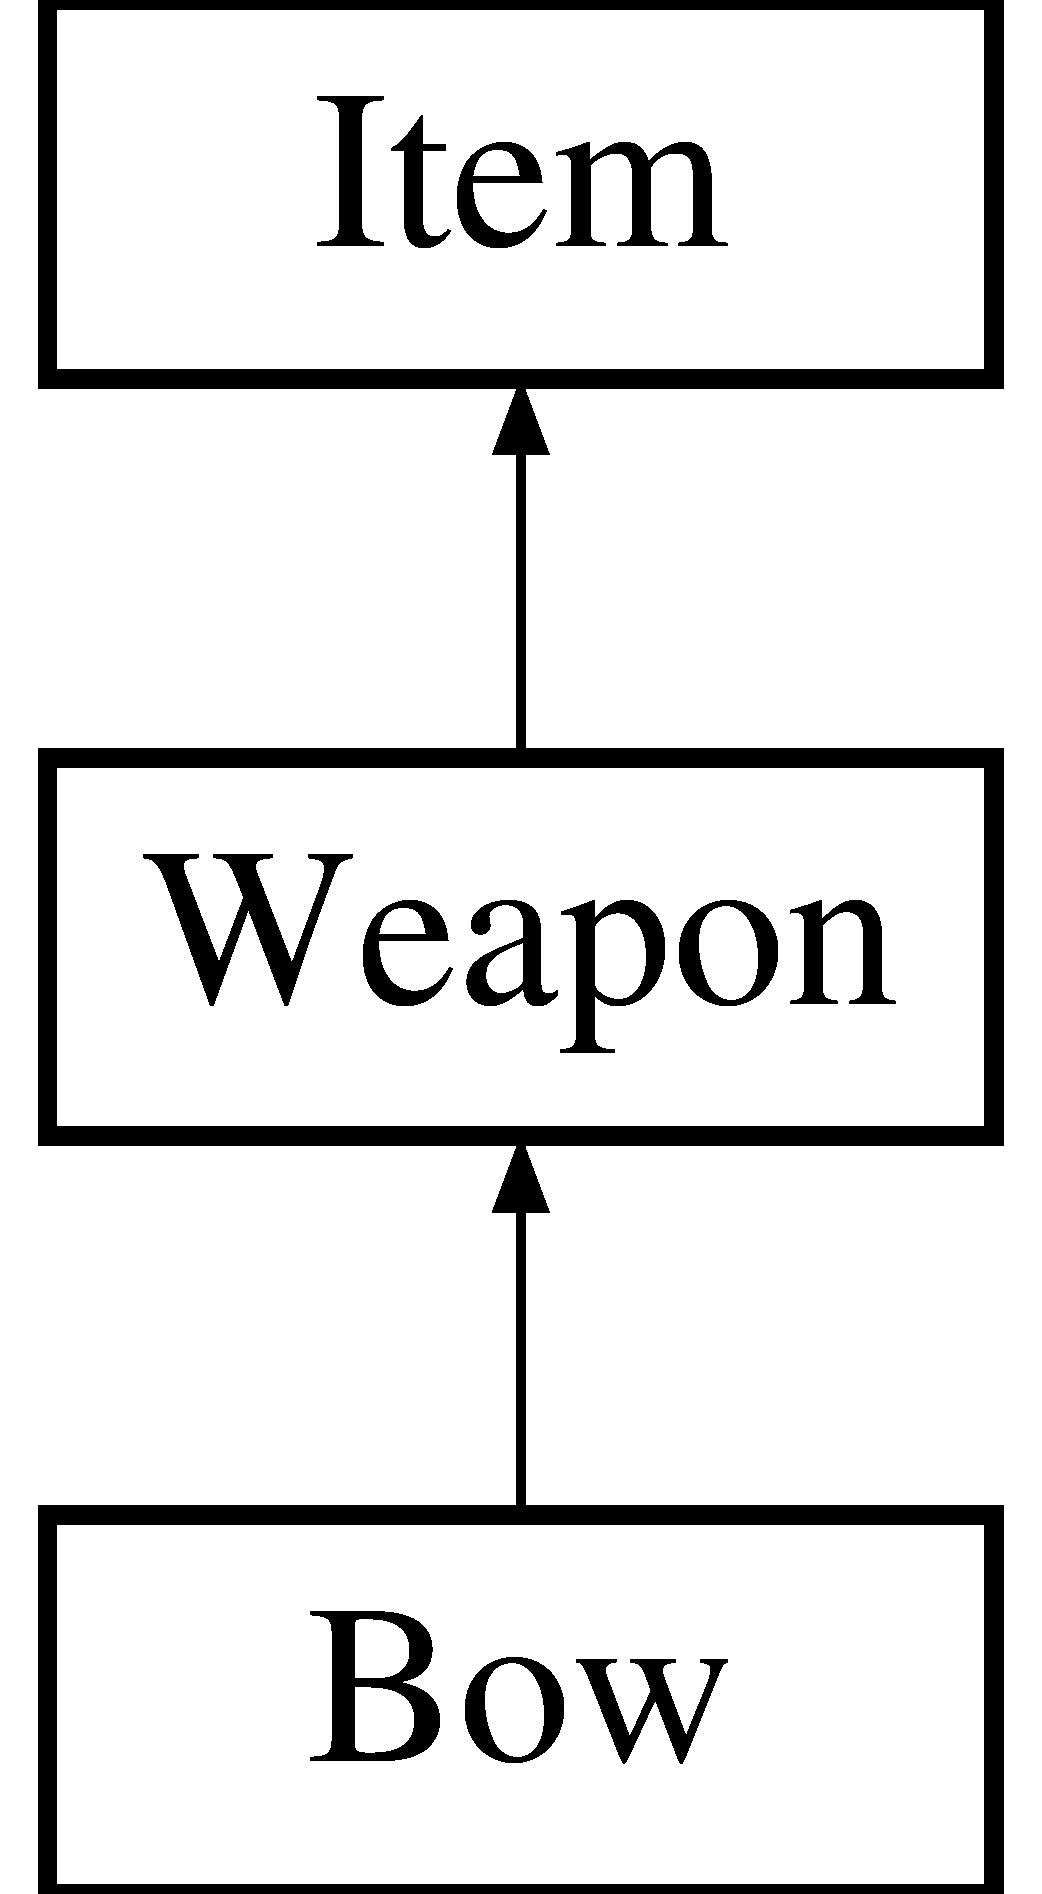
\includegraphics[height=3.000000cm]{classBow}
\end{center}
\end{figure}
\subsection*{Public Member Functions}
\begin{DoxyCompactItemize}
\item 
void \hyperlink{classBow_acdca55097e449415445fdcbda11037c8}{use} (\hyperlink{classCharacter}{Character} $\ast$target)
\end{DoxyCompactItemize}
\subsection*{Additional Inherited Members}


\subsection{Detailed Description}
Subclass of \hyperlink{classWeapon}{Weapon} to represent a bow in game. 

\subsection{Member Function Documentation}
\hypertarget{classBow_acdca55097e449415445fdcbda11037c8}{\index{Bow@{Bow}!use@{use}}
\index{use@{use}!Bow@{Bow}}
\subsubsection[{use}]{\setlength{\rightskip}{0pt plus 5cm}void Bow\-::use (
\begin{DoxyParamCaption}
\item[{{\bf Character} $\ast$}]{target}
\end{DoxyParamCaption}
)}}\label{classBow_acdca55097e449415445fdcbda11037c8}
Defines what happens when the spell is used 
\begin{DoxyParams}[1]{Parameters}
\mbox{\tt in}  & {\em target} & The character that the spell is used on \\
\hline
\end{DoxyParams}


The documentation for this class was generated from the following file\-:\begin{DoxyCompactItemize}
\item 
Item/My\-Weapons.\-h\end{DoxyCompactItemize}

\hypertarget{classCharacter}{\section{Character Class Reference}
\label{classCharacter}\index{Character@{Character}}
}


Abstract base class of \hyperlink{classNpc}{Npc}'s and \hyperlink{classPlayer}{Player}'s attributes.  




{\ttfamily \#include $<$Character.\-h$>$}

Inheritance diagram for Character\-:\begin{figure}[H]
\begin{center}
\leavevmode
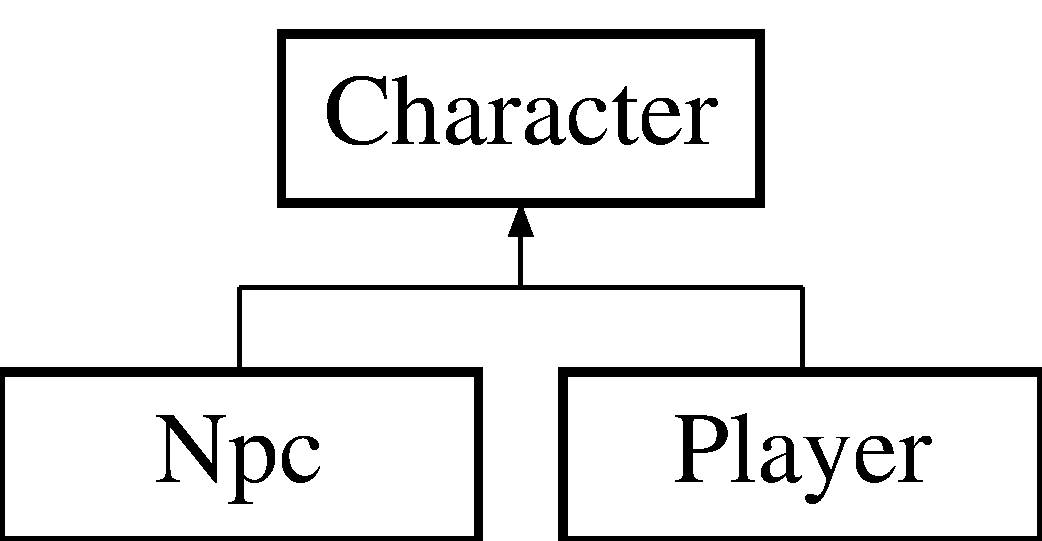
\includegraphics[height=2.000000cm]{classCharacter}
\end{center}
\end{figure}
\subsection*{Public Member Functions}
\begin{DoxyCompactItemize}
\item 
\hyperlink{classCharacter_adc27bdd255876169bad2ed0bae0cffb5}{Character} ()
\begin{DoxyCompactList}\small\item\em \hyperlink{classCharacter}{Character} constructor. \end{DoxyCompactList}\item 
virtual \hyperlink{classCharacter_a9e9be564d05ded80962b2045aa70b3fc}{$\sim$\-Character} ()
\begin{DoxyCompactList}\small\item\em \hyperlink{classCharacter}{Character} deconstructor. \end{DoxyCompactList}\item 
\hyperlink{classCharacter_a40d65bfcf0422cebc44b2e9b01d8fa2b}{Character} (const \hyperlink{classCharacter}{Character} \&)
\begin{DoxyCompactList}\small\item\em Const copy constructor. \end{DoxyCompactList}\item 
\hyperlink{classCharacter_a01a01e1feb04b92658d35e946ae155bb}{Character} (\hyperlink{classCharacter}{Character} \&)
\begin{DoxyCompactList}\small\item\em Copy constructor. \end{DoxyCompactList}\item 
\hyperlink{classCharacter}{Character} \& \hyperlink{classCharacter_aa441f0489c055e79c8dfdd813a20c3ad}{operator=} (const \hyperlink{classCharacter}{Character} \&p)
\begin{DoxyCompactList}\small\item\em Assignment operator overloader for copy constructor. \end{DoxyCompactList}\item 
virtual void \hyperlink{classCharacter_a546635f47f379e4eed59d85d31d85c86}{Fill\-Inventory} (\hyperlink{classItem}{Item} $\ast$item)
\item 
virtual vector$<$ \hyperlink{classItem}{Item} $\ast$ $>$ \hyperlink{classCharacter_a21e35b07fd2bddd94de754f5b8027fcc}{Get\-Inventory\-Items} ()
\item 
virtual \hyperlink{classItem}{Item} $\ast$ \hyperlink{classCharacter_ad13bd70e837024c6f185675d07d28f30}{Use\-Item} (string item)
\item 
virtual void \hyperlink{classCharacter_a5d8e04c875df744a3ea1ca426f8c0e12}{Change\-Gold} (int gold\-Mod)
\item 
virtual void \hyperlink{classCharacter_af0c41714e3a2cb65268fa721846a4939}{Change\-Health} (int h\-Mod)
\item 
virtual void \hyperlink{classCharacter_a50324e5ccb52512dfc69b3775d85c3dc}{Change\-Stamina} (int s\-Mod)
\item 
virtual int \hyperlink{classCharacter_aa443cb1d657be7a60225e02f46210c0d}{Get\-Stamina} () const 
\item 
virtual int \hyperlink{classCharacter_a85ce5d70120b39b72363ce9901e3ce70}{Get\-Gold} () const 
\item 
virtual int \hyperlink{classCharacter_a0e4d78d1bdebed299d4caa36f2d70209}{Get\-Health} () const 
\begin{DoxyCompactList}\small\item\em /return the health value of the character \end{DoxyCompactList}\item 
virtual \hyperlink{classImportImg}{Import\-Img} \& \hyperlink{classCharacter_a49cd0fdb0fc9e0f824aa54909ca86b2b}{Img} ()
\item 
virtual void \hyperlink{classCharacter_a2194329f9956a07b9e3dc021da93358e}{Draw} (\hyperlink{classScreen}{Screen} \&screen)
\item 
void \hyperlink{classCharacter_a0a69dd77da3407e50adc18e04cf2023b}{Empty\-Inventory} ()
\begin{DoxyCompactList}\small\item\em Helper function for the destructor to delete inventory items. \end{DoxyCompactList}\end{DoxyCompactItemize}
\subsection*{Protected Attributes}
\begin{DoxyCompactItemize}
\item 
\hyperlink{classImportImg}{Import\-Img} \hyperlink{classCharacter_a3a0a90b2a43858b259912f659b8e0eea}{img}
\item 
vector$<$ \hyperlink{classItem}{Item} $\ast$ $>$ \hyperlink{classCharacter_a27634c9cfd5a0cac96864b08b926c8a8}{inventory}
\begin{DoxyCompactList}\small\item\em Vector of items the character has. \end{DoxyCompactList}\item 
int \hyperlink{classCharacter_ab8dd866071dba429a35555e0c372e162}{gold}
\begin{DoxyCompactList}\small\item\em Amount of gold player has. \end{DoxyCompactList}\item 
int \hyperlink{classCharacter_a69c649b8febd22729e6edafb27e69aeb}{health}
\begin{DoxyCompactList}\small\item\em Characters health. \end{DoxyCompactList}\item 
int \hyperlink{classCharacter_a0f17daa14530e07f0ca479c2dd97f38b}{stamina}
\begin{DoxyCompactList}\small\item\em Characters stamina. \end{DoxyCompactList}\end{DoxyCompactItemize}


\subsection{Detailed Description}
Abstract base class of \hyperlink{classNpc}{Npc}'s and \hyperlink{classPlayer}{Player}'s attributes. 

\subsection{Constructor \& Destructor Documentation}
\hypertarget{classCharacter_adc27bdd255876169bad2ed0bae0cffb5}{\index{Character@{Character}!Character@{Character}}
\index{Character@{Character}!Character@{Character}}
\subsubsection[{Character}]{\setlength{\rightskip}{0pt plus 5cm}Character\-::\-Character (
\begin{DoxyParamCaption}
{}
\end{DoxyParamCaption}
)}}\label{classCharacter_adc27bdd255876169bad2ed0bae0cffb5}


\hyperlink{classCharacter}{Character} constructor. 

\hypertarget{classCharacter_a9e9be564d05ded80962b2045aa70b3fc}{\index{Character@{Character}!$\sim$\-Character@{$\sim$\-Character}}
\index{$\sim$\-Character@{$\sim$\-Character}!Character@{Character}}
\subsubsection[{$\sim$\-Character}]{\setlength{\rightskip}{0pt plus 5cm}Character\-::$\sim$\-Character (
\begin{DoxyParamCaption}
{}
\end{DoxyParamCaption}
)\hspace{0.3cm}{\ttfamily [virtual]}}}\label{classCharacter_a9e9be564d05ded80962b2045aa70b3fc}


\hyperlink{classCharacter}{Character} deconstructor. 

\hypertarget{classCharacter_a40d65bfcf0422cebc44b2e9b01d8fa2b}{\index{Character@{Character}!Character@{Character}}
\index{Character@{Character}!Character@{Character}}
\subsubsection[{Character}]{\setlength{\rightskip}{0pt plus 5cm}Character\-::\-Character (
\begin{DoxyParamCaption}
\item[{const {\bf Character} \&}]{p}
\end{DoxyParamCaption}
)}}\label{classCharacter_a40d65bfcf0422cebc44b2e9b01d8fa2b}


Const copy constructor. 

\hypertarget{classCharacter_a01a01e1feb04b92658d35e946ae155bb}{\index{Character@{Character}!Character@{Character}}
\index{Character@{Character}!Character@{Character}}
\subsubsection[{Character}]{\setlength{\rightskip}{0pt plus 5cm}Character\-::\-Character (
\begin{DoxyParamCaption}
\item[{{\bf Character} \&}]{p}
\end{DoxyParamCaption}
)}}\label{classCharacter_a01a01e1feb04b92658d35e946ae155bb}


Copy constructor. 



\subsection{Member Function Documentation}
\hypertarget{classCharacter_a5d8e04c875df744a3ea1ca426f8c0e12}{\index{Character@{Character}!Change\-Gold@{Change\-Gold}}
\index{Change\-Gold@{Change\-Gold}!Character@{Character}}
\subsubsection[{Change\-Gold}]{\setlength{\rightskip}{0pt plus 5cm}void Character\-::\-Change\-Gold (
\begin{DoxyParamCaption}
\item[{int}]{gold\-Mod}
\end{DoxyParamCaption}
)\hspace{0.3cm}{\ttfamily [virtual]}}}\label{classCharacter_a5d8e04c875df744a3ea1ca426f8c0e12}
Change the amount of gold a character has 
\begin{DoxyParams}[1]{Parameters}
\mbox{\tt in}  & {\em gold\-Mod,how} & much the current gold will be changed by \\
\hline
\end{DoxyParams}
\hypertarget{classCharacter_af0c41714e3a2cb65268fa721846a4939}{\index{Character@{Character}!Change\-Health@{Change\-Health}}
\index{Change\-Health@{Change\-Health}!Character@{Character}}
\subsubsection[{Change\-Health}]{\setlength{\rightskip}{0pt plus 5cm}void Character\-::\-Change\-Health (
\begin{DoxyParamCaption}
\item[{int}]{h\-Mod}
\end{DoxyParamCaption}
)\hspace{0.3cm}{\ttfamily [virtual]}}}\label{classCharacter_af0c41714e3a2cb65268fa721846a4939}
Changes the characters health 
\begin{DoxyParams}[1]{Parameters}
\mbox{\tt in}  & {\em h\-Mod,how} & the current health will be modified \\
\hline
\end{DoxyParams}
\hypertarget{classCharacter_a50324e5ccb52512dfc69b3775d85c3dc}{\index{Character@{Character}!Change\-Stamina@{Change\-Stamina}}
\index{Change\-Stamina@{Change\-Stamina}!Character@{Character}}
\subsubsection[{Change\-Stamina}]{\setlength{\rightskip}{0pt plus 5cm}void Character\-::\-Change\-Stamina (
\begin{DoxyParamCaption}
\item[{int}]{s\-Mod}
\end{DoxyParamCaption}
)\hspace{0.3cm}{\ttfamily [virtual]}}}\label{classCharacter_a50324e5ccb52512dfc69b3775d85c3dc}
Changes players stamina 
\begin{DoxyParams}[1]{Parameters}
\mbox{\tt in}  & {\em s\-Mod,how} & the curent stamina will be modified \\
\hline
\end{DoxyParams}
\hypertarget{classCharacter_a2194329f9956a07b9e3dc021da93358e}{\index{Character@{Character}!Draw@{Draw}}
\index{Draw@{Draw}!Character@{Character}}
\subsubsection[{Draw}]{\setlength{\rightskip}{0pt plus 5cm}void Character\-::\-Draw (
\begin{DoxyParamCaption}
\item[{{\bf Screen} \&}]{screen}
\end{DoxyParamCaption}
)\hspace{0.3cm}{\ttfamily [virtual]}}}\label{classCharacter_a2194329f9956a07b9e3dc021da93358e}
Draw the player 
\begin{DoxyParams}[1]{Parameters}
\mbox{\tt in}  & {\em screen,a} & reference to the screen \\
\hline
\end{DoxyParams}
\hypertarget{classCharacter_a0a69dd77da3407e50adc18e04cf2023b}{\index{Character@{Character}!Empty\-Inventory@{Empty\-Inventory}}
\index{Empty\-Inventory@{Empty\-Inventory}!Character@{Character}}
\subsubsection[{Empty\-Inventory}]{\setlength{\rightskip}{0pt plus 5cm}void Character\-::\-Empty\-Inventory (
\begin{DoxyParamCaption}
{}
\end{DoxyParamCaption}
)}}\label{classCharacter_a0a69dd77da3407e50adc18e04cf2023b}


Helper function for the destructor to delete inventory items. 

\hypertarget{classCharacter_a546635f47f379e4eed59d85d31d85c86}{\index{Character@{Character}!Fill\-Inventory@{Fill\-Inventory}}
\index{Fill\-Inventory@{Fill\-Inventory}!Character@{Character}}
\subsubsection[{Fill\-Inventory}]{\setlength{\rightskip}{0pt plus 5cm}void Character\-::\-Fill\-Inventory (
\begin{DoxyParamCaption}
\item[{{\bf Item} $\ast$}]{item}
\end{DoxyParamCaption}
)\hspace{0.3cm}{\ttfamily [virtual]}}}\label{classCharacter_a546635f47f379e4eed59d85d31d85c86}
Function to fill the characters inventory 
\begin{DoxyParams}[1]{Parameters}
\mbox{\tt in}  & {\em item,a} & pointer to the item being added into inventory \\
\hline
\end{DoxyParams}
\hypertarget{classCharacter_a85ce5d70120b39b72363ce9901e3ce70}{\index{Character@{Character}!Get\-Gold@{Get\-Gold}}
\index{Get\-Gold@{Get\-Gold}!Character@{Character}}
\subsubsection[{Get\-Gold}]{\setlength{\rightskip}{0pt plus 5cm}virtual int Character\-::\-Get\-Gold (
\begin{DoxyParamCaption}
{}
\end{DoxyParamCaption}
) const\hspace{0.3cm}{\ttfamily [inline]}, {\ttfamily [virtual]}}}\label{classCharacter_a85ce5d70120b39b72363ce9901e3ce70}
\begin{DoxyReturn}{Returns}
the gold value of the character 
\end{DoxyReturn}
\hypertarget{classCharacter_a0e4d78d1bdebed299d4caa36f2d70209}{\index{Character@{Character}!Get\-Health@{Get\-Health}}
\index{Get\-Health@{Get\-Health}!Character@{Character}}
\subsubsection[{Get\-Health}]{\setlength{\rightskip}{0pt plus 5cm}virtual int Character\-::\-Get\-Health (
\begin{DoxyParamCaption}
{}
\end{DoxyParamCaption}
) const\hspace{0.3cm}{\ttfamily [inline]}, {\ttfamily [virtual]}}}\label{classCharacter_a0e4d78d1bdebed299d4caa36f2d70209}


/return the health value of the character 

\hypertarget{classCharacter_a21e35b07fd2bddd94de754f5b8027fcc}{\index{Character@{Character}!Get\-Inventory\-Items@{Get\-Inventory\-Items}}
\index{Get\-Inventory\-Items@{Get\-Inventory\-Items}!Character@{Character}}
\subsubsection[{Get\-Inventory\-Items}]{\setlength{\rightskip}{0pt plus 5cm}vector$<$ {\bf Item} $\ast$ $>$ Character\-::\-Get\-Inventory\-Items (
\begin{DoxyParamCaption}
{}
\end{DoxyParamCaption}
)\hspace{0.3cm}{\ttfamily [virtual]}}}\label{classCharacter_a21e35b07fd2bddd94de754f5b8027fcc}
Shows a list of inventory items \begin{DoxyReturn}{Returns}
, a the vector of the inventory 
\end{DoxyReturn}
\hypertarget{classCharacter_aa443cb1d657be7a60225e02f46210c0d}{\index{Character@{Character}!Get\-Stamina@{Get\-Stamina}}
\index{Get\-Stamina@{Get\-Stamina}!Character@{Character}}
\subsubsection[{Get\-Stamina}]{\setlength{\rightskip}{0pt plus 5cm}virtual int Character\-::\-Get\-Stamina (
\begin{DoxyParamCaption}
{}
\end{DoxyParamCaption}
) const\hspace{0.3cm}{\ttfamily [inline]}, {\ttfamily [virtual]}}}\label{classCharacter_aa443cb1d657be7a60225e02f46210c0d}
\begin{DoxyReturn}{Returns}
the stamina value of the character 
\end{DoxyReturn}
\hypertarget{classCharacter_a49cd0fdb0fc9e0f824aa54909ca86b2b}{\index{Character@{Character}!Img@{Img}}
\index{Img@{Img}!Character@{Character}}
\subsubsection[{Img}]{\setlength{\rightskip}{0pt plus 5cm}virtual {\bf Import\-Img}\& Character\-::\-Img (
\begin{DoxyParamCaption}
{}
\end{DoxyParamCaption}
)\hspace{0.3cm}{\ttfamily [inline]}, {\ttfamily [virtual]}}}\label{classCharacter_a49cd0fdb0fc9e0f824aa54909ca86b2b}
\begin{DoxyReturn}{Returns}
the image representing the character 
\end{DoxyReturn}
\hypertarget{classCharacter_aa441f0489c055e79c8dfdd813a20c3ad}{\index{Character@{Character}!operator=@{operator=}}
\index{operator=@{operator=}!Character@{Character}}
\subsubsection[{operator=}]{\setlength{\rightskip}{0pt plus 5cm}{\bf Character} \& Character\-::operator= (
\begin{DoxyParamCaption}
\item[{const {\bf Character} \&}]{p}
\end{DoxyParamCaption}
)}}\label{classCharacter_aa441f0489c055e79c8dfdd813a20c3ad}


Assignment operator overloader for copy constructor. 

\hypertarget{classCharacter_ad13bd70e837024c6f185675d07d28f30}{\index{Character@{Character}!Use\-Item@{Use\-Item}}
\index{Use\-Item@{Use\-Item}!Character@{Character}}
\subsubsection[{Use\-Item}]{\setlength{\rightskip}{0pt plus 5cm}{\bf Item} $\ast$ Character\-::\-Use\-Item (
\begin{DoxyParamCaption}
\item[{string}]{item}
\end{DoxyParamCaption}
)\hspace{0.3cm}{\ttfamily [virtual]}}}\label{classCharacter_ad13bd70e837024c6f185675d07d28f30}
Chooses the item to be used 
\begin{DoxyParams}[1]{Parameters}
\mbox{\tt in}  & {\em item,the} & item name to be found in the inventory vector \\
\hline
\end{DoxyParams}
\begin{DoxyReturn}{Returns}
\hyperlink{classItem}{Item}, a pointer to an item if its found in the inventory 
\end{DoxyReturn}


\subsection{Member Data Documentation}
\hypertarget{classCharacter_ab8dd866071dba429a35555e0c372e162}{\index{Character@{Character}!gold@{gold}}
\index{gold@{gold}!Character@{Character}}
\subsubsection[{gold}]{\setlength{\rightskip}{0pt plus 5cm}int Character\-::gold\hspace{0.3cm}{\ttfamily [protected]}}}\label{classCharacter_ab8dd866071dba429a35555e0c372e162}


Amount of gold player has. 

\hypertarget{classCharacter_a69c649b8febd22729e6edafb27e69aeb}{\index{Character@{Character}!health@{health}}
\index{health@{health}!Character@{Character}}
\subsubsection[{health}]{\setlength{\rightskip}{0pt plus 5cm}int Character\-::health\hspace{0.3cm}{\ttfamily [protected]}}}\label{classCharacter_a69c649b8febd22729e6edafb27e69aeb}


Characters health. 

\hypertarget{classCharacter_a3a0a90b2a43858b259912f659b8e0eea}{\index{Character@{Character}!img@{img}}
\index{img@{img}!Character@{Character}}
\subsubsection[{img}]{\setlength{\rightskip}{0pt plus 5cm}{\bf Import\-Img} Character\-::img\hspace{0.3cm}{\ttfamily [protected]}}}\label{classCharacter_a3a0a90b2a43858b259912f659b8e0eea}
\hypertarget{classCharacter_a27634c9cfd5a0cac96864b08b926c8a8}{\index{Character@{Character}!inventory@{inventory}}
\index{inventory@{inventory}!Character@{Character}}
\subsubsection[{inventory}]{\setlength{\rightskip}{0pt plus 5cm}vector$<$ {\bf Item}$\ast$ $>$ Character\-::inventory\hspace{0.3cm}{\ttfamily [protected]}}}\label{classCharacter_a27634c9cfd5a0cac96864b08b926c8a8}


Vector of items the character has. 

\hypertarget{classCharacter_a0f17daa14530e07f0ca479c2dd97f38b}{\index{Character@{Character}!stamina@{stamina}}
\index{stamina@{stamina}!Character@{Character}}
\subsubsection[{stamina}]{\setlength{\rightskip}{0pt plus 5cm}int Character\-::stamina\hspace{0.3cm}{\ttfamily [protected]}}}\label{classCharacter_a0f17daa14530e07f0ca479c2dd97f38b}


Characters stamina. 



The documentation for this class was generated from the following files\-:\begin{DoxyCompactItemize}
\item 
/home/rigt2720/\-Kodika/\-Character/\hyperlink{Character_8h}{Character.\-h}\item 
/home/rigt2720/\-Kodika/\-Character/\hyperlink{Character_8cpp}{Character.\-cpp}\end{DoxyCompactItemize}

\hypertarget{classCharacterMenu}{\section{Character\-Menu Class Reference}
\label{classCharacterMenu}\index{Character\-Menu@{Character\-Menu}}
}
Inheritance diagram for Character\-Menu\-:\begin{figure}[H]
\begin{center}
\leavevmode
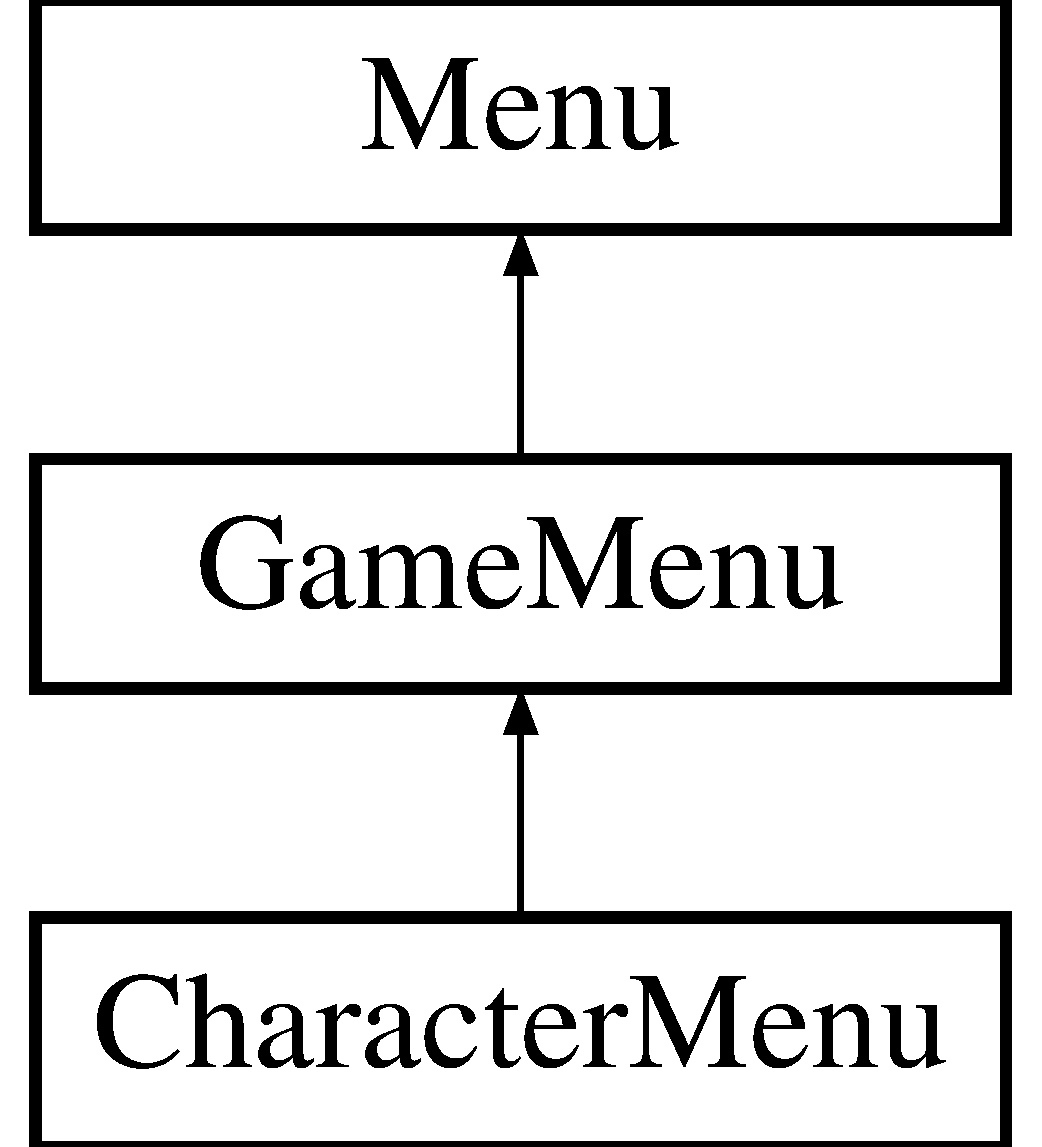
\includegraphics[height=3.000000cm]{classCharacterMenu}
\end{center}
\end{figure}
\subsection*{Public Member Functions}
\begin{DoxyCompactItemize}
\item 
\hypertarget{classCharacterMenu_a1cccb5ffc144797bd6472e0839c38c03}{\hyperlink{classCharacterMenu_a1cccb5ffc144797bd6472e0839c38c03}{Character\-Menu} ()}\label{classCharacterMenu_a1cccb5ffc144797bd6472e0839c38c03}

\begin{DoxyCompactList}\small\item\em This is the default constructor. \end{DoxyCompactList}\item 
\hypertarget{classCharacterMenu_a6e7e278406e10cd6eb0f3d5aea5fb4b2}{virtual \hyperlink{classCharacterMenu_a6e7e278406e10cd6eb0f3d5aea5fb4b2}{$\sim$\-Character\-Menu} ()}\label{classCharacterMenu_a6e7e278406e10cd6eb0f3d5aea5fb4b2}

\begin{DoxyCompactList}\small\item\em This is the virtual destructor. \end{DoxyCompactList}\item 
virtual void \hyperlink{classCharacterMenu_a374493bc5b1e04b13647482c98df5fd6}{Set\-Options} (map$<$ string $>$ options\-List, string type)
\item 
virtual void \hyperlink{classCharacterMenu_a7a9163eec7ac69aeb5431869a0675646}{Handle\-Input} (istream \&is)
\end{DoxyCompactItemize}
\subsection*{Additional Inherited Members}


\subsection{Member Function Documentation}
\hypertarget{classCharacterMenu_a7a9163eec7ac69aeb5431869a0675646}{\index{Character\-Menu@{Character\-Menu}!Handle\-Input@{Handle\-Input}}
\index{Handle\-Input@{Handle\-Input}!CharacterMenu@{Character\-Menu}}
\subsubsection[{Handle\-Input}]{\setlength{\rightskip}{0pt plus 5cm}virtual void Character\-Menu\-::\-Handle\-Input (
\begin{DoxyParamCaption}
\item[{istream \&}]{is}
\end{DoxyParamCaption}
)\hspace{0.3cm}{\ttfamily [virtual]}}}\label{classCharacterMenu_a7a9163eec7ac69aeb5431869a0675646}
This function handles the input for the menu options. 
\begin{DoxyParams}[1]{Parameters}
\mbox{\tt in,out}  & {\em is} & The in-\/stream operator to read the input. \\
\hline
\end{DoxyParams}


Implements \hyperlink{classGameMenu_a02ba09feedece5773f44ba865ccffb42}{Game\-Menu}.

\hypertarget{classCharacterMenu_a374493bc5b1e04b13647482c98df5fd6}{\index{Character\-Menu@{Character\-Menu}!Set\-Options@{Set\-Options}}
\index{Set\-Options@{Set\-Options}!CharacterMenu@{Character\-Menu}}
\subsubsection[{Set\-Options}]{\setlength{\rightskip}{0pt plus 5cm}virtual void Character\-Menu\-::\-Set\-Options (
\begin{DoxyParamCaption}
\item[{map$<$ string $>$}]{options\-List, }
\item[{string}]{type}
\end{DoxyParamCaption}
)\hspace{0.3cm}{\ttfamily [virtual]}}}\label{classCharacterMenu_a374493bc5b1e04b13647482c98df5fd6}
This function sets the specific options for the \hyperlink{classMenu}{Menu} type. 
\begin{DoxyParams}[1]{Parameters}
\mbox{\tt in}  & {\em Options\-List} & A map of all the options for the current menu. Each option has a unique key to make input easier. \\
\hline
\mbox{\tt in}  & {\em type} & This denotes the type of menu to display. \\
\hline
\end{DoxyParams}


Implements \hyperlink{classGameMenu_a25172d8d311df4f7b79074d60f74642e}{Game\-Menu}.



The documentation for this class was generated from the following file\-:\begin{DoxyCompactItemize}
\item 
Menu/Character\-Menu.\-h\end{DoxyCompactItemize}

\hypertarget{classCodeCracker}{\section{Code\-Cracker Class Reference}
\label{classCodeCracker}\index{Code\-Cracker@{Code\-Cracker}}
}


This class contains the mini-\/game/puzzle Code Cracker.  




{\ttfamily \#include $<$code\-\_\-cracker.\-h$>$}

Inheritance diagram for Code\-Cracker\-:\begin{figure}[H]
\begin{center}
\leavevmode
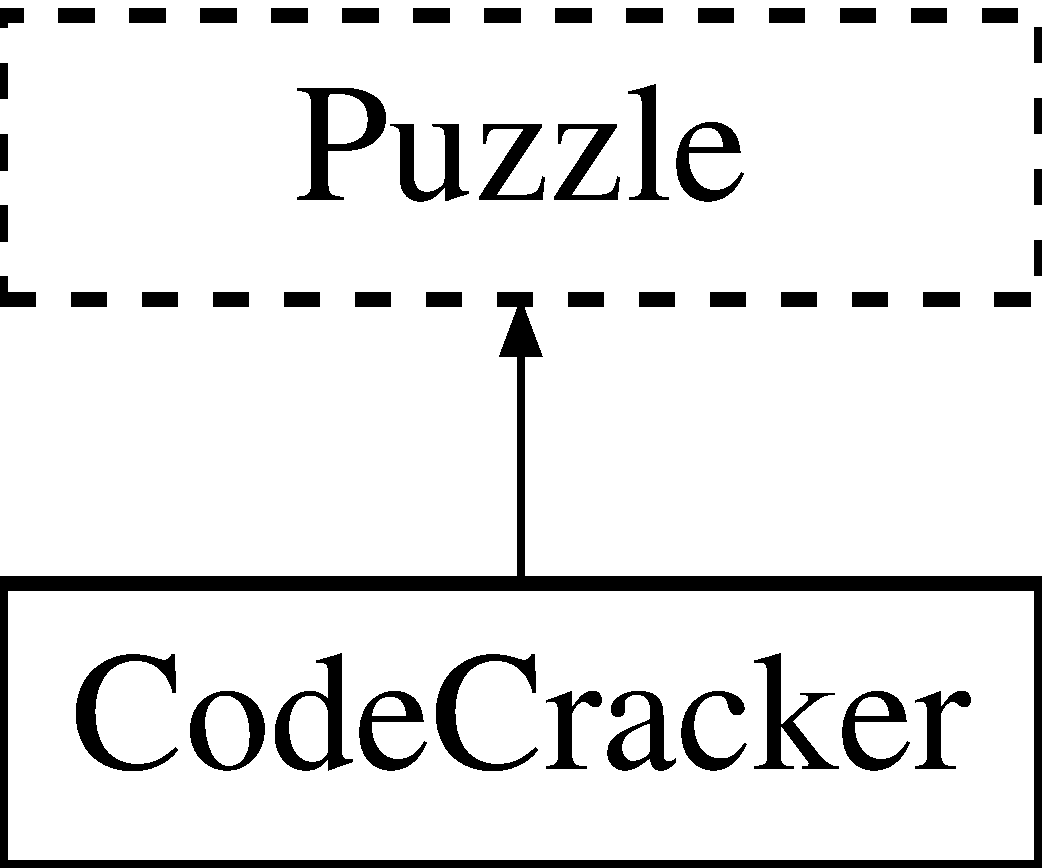
\includegraphics[height=2.000000cm]{classCodeCracker}
\end{center}
\end{figure}
\subsection*{Public Member Functions}
\begin{DoxyCompactItemize}
\item 
\hypertarget{classCodeCracker_a46b5ec438efd38104b9a406b45c8cd68}{\hyperlink{classCodeCracker_a46b5ec438efd38104b9a406b45c8cd68}{Code\-Cracker} ()}\label{classCodeCracker_a46b5ec438efd38104b9a406b45c8cd68}

\begin{DoxyCompactList}\small\item\em Default constructor for hanoi, reads in riddles from .txt files. \end{DoxyCompactList}\item 
\hypertarget{classCodeCracker_ae7dc389e166286ca2271625154dde39c}{\hyperlink{classCodeCracker_ae7dc389e166286ca2271625154dde39c}{$\sim$\-Code\-Cracker} ()}\label{classCodeCracker_ae7dc389e166286ca2271625154dde39c}

\begin{DoxyCompactList}\small\item\em Deconstructor. \end{DoxyCompactList}\item 
void \hyperlink{classCodeCracker_a4f2aaaf60b31cf33cc0d70622665be45}{Run\-Game} ()
\item 
\hypertarget{classCodeCracker_a46b5ec438efd38104b9a406b45c8cd68}{\hyperlink{classCodeCracker_a46b5ec438efd38104b9a406b45c8cd68}{Code\-Cracker} ()}\label{classCodeCracker_a46b5ec438efd38104b9a406b45c8cd68}

\begin{DoxyCompactList}\small\item\em Default constructor for hanoi, reads in riddles from .txt files. \end{DoxyCompactList}\item 
\hypertarget{classCodeCracker_ae7dc389e166286ca2271625154dde39c}{\hyperlink{classCodeCracker_ae7dc389e166286ca2271625154dde39c}{$\sim$\-Code\-Cracker} ()}\label{classCodeCracker_ae7dc389e166286ca2271625154dde39c}

\begin{DoxyCompactList}\small\item\em Deconstructor. \end{DoxyCompactList}\item 
void \hyperlink{classCodeCracker_a4f2aaaf60b31cf33cc0d70622665be45}{Run\-Game} ()
\end{DoxyCompactItemize}


\subsection{Detailed Description}
This class contains the mini-\/game/puzzle Code Cracker. 

\begin{DoxyAuthor}{Author}
Tyler Siwy 
\end{DoxyAuthor}
\begin{DoxyDate}{Date}
Oct 20, 2017 
\end{DoxyDate}


\subsection{Member Function Documentation}
\hypertarget{classCodeCracker_a4f2aaaf60b31cf33cc0d70622665be45}{\index{Code\-Cracker@{Code\-Cracker}!Run\-Game@{Run\-Game}}
\index{Run\-Game@{Run\-Game}!CodeCracker@{Code\-Cracker}}
\subsubsection[{Run\-Game}]{\setlength{\rightskip}{0pt plus 5cm}void Code\-Cracker\-::\-Run\-Game (
\begin{DoxyParamCaption}
{}
\end{DoxyParamCaption}
)\hspace{0.3cm}{\ttfamily [virtual]}}}\label{classCodeCracker_a4f2aaaf60b31cf33cc0d70622665be45}
Method to run the game, serves as a 'main' for the mini-\/game, calling functions from private until the player has won. 

Reimplemented from \hyperlink{classPuzzle_a0962210916279dc1368b695b399c8ea6}{Puzzle}.

\hypertarget{classCodeCracker_a4f2aaaf60b31cf33cc0d70622665be45}{\index{Code\-Cracker@{Code\-Cracker}!Run\-Game@{Run\-Game}}
\index{Run\-Game@{Run\-Game}!CodeCracker@{Code\-Cracker}}
\subsubsection[{Run\-Game}]{\setlength{\rightskip}{0pt plus 5cm}void Code\-Cracker\-::\-Run\-Game (
\begin{DoxyParamCaption}
{}
\end{DoxyParamCaption}
)\hspace{0.3cm}{\ttfamily [virtual]}}}\label{classCodeCracker_a4f2aaaf60b31cf33cc0d70622665be45}
Method to run the game, serves as a 'main' for the mini-\/game, calling functions from private until the player has won. 

Reimplemented from \hyperlink{classPuzzle_a0962210916279dc1368b695b399c8ea6}{Puzzle}.



The documentation for this class was generated from the following files\-:\begin{DoxyCompactItemize}
\item 
Puzzles/code\-\_\-cracker.\-h\item 
Puzzles/Code\-Cracker.\-h\end{DoxyCompactItemize}

\hypertarget{classConnectFour}{\section{Connect\-Four Class Reference}
\label{classConnectFour}\index{Connect\-Four@{Connect\-Four}}
}


This class contains the mini-\/game/puzzle Connect Four.  




{\ttfamily \#include $<$Connect\-Four.\-h$>$}

Inheritance diagram for Connect\-Four\-:\begin{figure}[H]
\begin{center}
\leavevmode
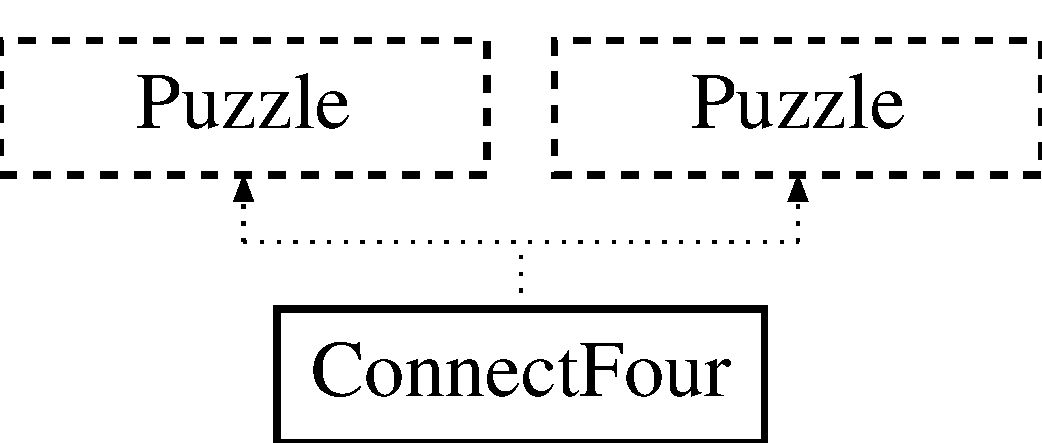
\includegraphics[height=2.000000cm]{classConnectFour}
\end{center}
\end{figure}
\subsection*{Public Member Functions}
\begin{DoxyCompactItemize}
\item 
\hyperlink{classConnectFour_a9d7a0db424f22513386fa60ed2d5b575}{Connect\-Four} ()
\begin{DoxyCompactList}\small\item\em Default constructor for \hyperlink{classConnectFour}{Connect\-Four}, sets heigh to \-: and width to\-: \end{DoxyCompactList}\item 
virtual \hyperlink{classConnectFour_ae7d414d7f7f694fd427bfeaef80bd1f9}{$\sim$\-Connect\-Four} ()
\begin{DoxyCompactList}\small\item\em De-\/constructor. \end{DoxyCompactList}\item 
virtual void \hyperlink{classConnectFour_a3b578d1126bc575fa23b8811f121c8be}{Run\-Game} (\hyperlink{classCharacter}{Character} $\ast$player)
\end{DoxyCompactItemize}
\subsection*{Private Member Functions}
\begin{DoxyCompactItemize}
\item 
void \hyperlink{classConnectFour_a6bde7d38a9493ea5475a0a941f4c96df}{Move\-Piece} (char user\-Piece, int column)
\item 
void \hyperlink{classConnectFour_a618f3caa7db76bc8b4832a2338967a5b}{Play\-A\-I} (char Ai\-Piece)
\begin{DoxyCompactList}\small\item\em Performs the A\-I players move. \end{DoxyCompactList}\item 
bool \hyperlink{classConnectFour_a1cbd5ba040359e265c85a27407528915}{Valid\-Move} (int input)
\item 
bool \hyperlink{classConnectFour_a5e33120d5b6a49e8eacd976de8be9c7c}{Is\-Input\-Out\-Of\-Scope} (int input)
\item 
bool \hyperlink{classConnectFour_a4f7dd5550d9ba548c542d887822cc1f0}{Win\-Check} ()
\begin{DoxyCompactList}\small\item\em Checks to see if there have been any 4 tokens in a row in the grid vector. \end{DoxyCompactList}\item 
bool \hyperlink{classConnectFour_aad3b75c20b82a21fcbe648e7ee134a4b}{Horizontal\-Check} ()
\item 
bool \hyperlink{classConnectFour_afe5fd24730a5d1295c1bb20fc2e6c1a8}{Vertical\-Check} ()
\item 
bool \hyperlink{classConnectFour_acacb2e213d7c4f6dec2cf2f9d3c370f9}{Left\-Diagonal\-Check} ()
\item 
bool \hyperlink{classConnectFour_ac49d716bde974c19aab3e47e66d94073}{Right\-Diagonal\-Check} ()
\item 
bool \hyperlink{classConnectFour_a26d75c9c50d6424df11de765086edc8a}{Is\-Column\-Full} (int input)
\begin{DoxyCompactList}\small\item\em Function which checks if a column is full. \end{DoxyCompactList}\item 
bool \hyperlink{classConnectFour_a408b2a0222e08488c258e4225ba5b8f6}{Is\-Board\-Full} ()
\begin{DoxyCompactList}\small\item\em Returns true if every space in the board has been filled with a character. \end{DoxyCompactList}\item 
bool \hyperlink{classConnectFour_a6f356156a6c23ee1f5838cd96b3b84bc}{Tie\-Game\-Check} (int \&current\-Player)
\item 
void \hyperlink{classConnectFour_ad453f2707d1ae7bb87cdd2d46010d951}{Board\-Setup} ()
\begin{DoxyCompactList}\small\item\em Sets the board up for the beginning of the game, placing them in screen. \end{DoxyCompactList}\item 
void \hyperlink{classConnectFour_a735502158808aaa23f0a2d38ac3f841f}{End\-Game\-Prompt} (int \&current\-Player, \hyperlink{classConnectFourMenu}{Connect\-Four\-Menu} \&menu, \hyperlink{classCharacter}{Character} $\ast$player)
\item 
void \hyperlink{classConnectFour_aaf17855d2cec2d71c07614af530a00bf}{Reset\-Game} (int \&current\-Player)
\begin{DoxyCompactList}\small\item\em Resets the game for another round in the event that the A\-I wins. \end{DoxyCompactList}\item 
void \hyperlink{classConnectFour_a8f74f9d22c247508e868222c27136641}{Set\-Current\-Player\-Char} (int current\-Player)
\end{DoxyCompactItemize}
\subsection*{Private Attributes}
\begin{DoxyCompactItemize}
\item 
\hyperlink{classScreen}{Screen} \hyperlink{classConnectFour_a7548207e4c83260233e8d3668ae3e7e2}{Connect\-Four\-Screen}
\item 
std\-::vector$<$ vector$<$ char $>$ $>$ \hyperlink{classConnectFour_a42275b6a7a1b490b7e9adc3e2d5480d9}{grid}
\begin{DoxyCompactList}\small\item\em The vector which stores the gameboards chars. \end{DoxyCompactList}\item 
char \hyperlink{classConnectFour_adc938d715dbe28efc1db3b4a1dc866cb}{current\-Player\-Char}
\item 
int \hyperlink{classConnectFour_a9ebcc46eaaac1805eab8b90925f83a63}{x\-Size}
\item 
int \hyperlink{classConnectFour_acd39fbfa19a81ab05e7aae3ac51e9ed8}{y\-Size}
\end{DoxyCompactItemize}
\subsection*{Additional Inherited Members}


\subsection{Detailed Description}
This class contains the mini-\/game/puzzle Connect Four. 

\begin{DoxyAuthor}{Author}
Tyler Siwy 
\end{DoxyAuthor}
\begin{DoxyDate}{Date}
Oct 20, 2017 
\end{DoxyDate}


\subsection{Constructor \& Destructor Documentation}
\hypertarget{classConnectFour_a9d7a0db424f22513386fa60ed2d5b575}{\index{Connect\-Four@{Connect\-Four}!Connect\-Four@{Connect\-Four}}
\index{Connect\-Four@{Connect\-Four}!ConnectFour@{Connect\-Four}}
\subsubsection[{Connect\-Four}]{\setlength{\rightskip}{0pt plus 5cm}Connect\-Four\-::\-Connect\-Four (
\begin{DoxyParamCaption}
{}
\end{DoxyParamCaption}
)}}\label{classConnectFour_a9d7a0db424f22513386fa60ed2d5b575}


Default constructor for \hyperlink{classConnectFour}{Connect\-Four}, sets heigh to \-: and width to\-: 

\begin{DoxyAuthor}{Author}
Tyler Siwy 
\end{DoxyAuthor}
\begin{DoxyDate}{Date}
Nov 15, 2017 
\end{DoxyDate}
Setting up the game vector \hypertarget{classConnectFour_ae7d414d7f7f694fd427bfeaef80bd1f9}{\index{Connect\-Four@{Connect\-Four}!$\sim$\-Connect\-Four@{$\sim$\-Connect\-Four}}
\index{$\sim$\-Connect\-Four@{$\sim$\-Connect\-Four}!ConnectFour@{Connect\-Four}}
\subsubsection[{$\sim$\-Connect\-Four}]{\setlength{\rightskip}{0pt plus 5cm}Connect\-Four\-::$\sim$\-Connect\-Four (
\begin{DoxyParamCaption}
{}
\end{DoxyParamCaption}
)\hspace{0.3cm}{\ttfamily [virtual]}}}\label{classConnectFour_ae7d414d7f7f694fd427bfeaef80bd1f9}


De-\/constructor. 



\subsection{Member Function Documentation}
\hypertarget{classConnectFour_ad453f2707d1ae7bb87cdd2d46010d951}{\index{Connect\-Four@{Connect\-Four}!Board\-Setup@{Board\-Setup}}
\index{Board\-Setup@{Board\-Setup}!ConnectFour@{Connect\-Four}}
\subsubsection[{Board\-Setup}]{\setlength{\rightskip}{0pt plus 5cm}void Connect\-Four\-::\-Board\-Setup (
\begin{DoxyParamCaption}
{}
\end{DoxyParamCaption}
)\hspace{0.3cm}{\ttfamily [private]}}}\label{classConnectFour_ad453f2707d1ae7bb87cdd2d46010d951}


Sets the board up for the beginning of the game, placing them in screen. 

Sets up the board with the ui for the connect four game. If i is odd, fill the entire row with '-\/'

top\-Bound and left\-Bound should set the board centered inside the screen object.

If i is even, fill the row with squares to place tokens in later

top\-Bound and left\-Bound should set the board centered inside the screen object.

top\-Bound and left\-Bound should set the board centered inside the screen object. \hypertarget{classConnectFour_a735502158808aaa23f0a2d38ac3f841f}{\index{Connect\-Four@{Connect\-Four}!End\-Game\-Prompt@{End\-Game\-Prompt}}
\index{End\-Game\-Prompt@{End\-Game\-Prompt}!ConnectFour@{Connect\-Four}}
\subsubsection[{End\-Game\-Prompt}]{\setlength{\rightskip}{0pt plus 5cm}void Connect\-Four\-::\-End\-Game\-Prompt (
\begin{DoxyParamCaption}
\item[{int \&}]{current\-Player, }
\item[{{\bf Connect\-Four\-Menu} \&}]{menu, }
\item[{{\bf Character} $\ast$}]{player}
\end{DoxyParamCaption}
)\hspace{0.3cm}{\ttfamily [private]}}}\label{classConnectFour_a735502158808aaa23f0a2d38ac3f841f}
Prompts the player and handles the end of the game appropriately. 
\begin{DoxyParams}[1]{Parameters}
\mbox{\tt in}  & {\em current\-Player,assigned} & to be human for new game. \mbox{[}in\mbox{]} menu, the menu used to output stuffs \\
\hline
\mbox{\tt in}  & {\em player,a} & pointer to the player usd to modify stats\\
\hline
\end{DoxyParams}
If current\-Player is even, the A\-I has won, -\/1 player health, reset the game for another round until the player has won. \hypertarget{classConnectFour_aad3b75c20b82a21fcbe648e7ee134a4b}{\index{Connect\-Four@{Connect\-Four}!Horizontal\-Check@{Horizontal\-Check}}
\index{Horizontal\-Check@{Horizontal\-Check}!ConnectFour@{Connect\-Four}}
\subsubsection[{Horizontal\-Check}]{\setlength{\rightskip}{0pt plus 5cm}bool Connect\-Four\-::\-Horizontal\-Check (
\begin{DoxyParamCaption}
{}
\end{DoxyParamCaption}
)\hspace{0.3cm}{\ttfamily [private]}}}\label{classConnectFour_aad3b75c20b82a21fcbe648e7ee134a4b}
Checks the entire grid to see if there is 4 of a kind in the horizontal position, returns true if it finds 4 of a kind, false otherwise. at\-Count counts the number of '@' tokens in the line. copyright\-Count counts the number of '©' tokens in the line.

If an '@' token is found, reset the count for copyright since it is not consecutive anymore.

If a '\#' token is found, reset the count for at since it is not consecutive anymore.

If either count is at 4 then we have found four of a kind and a player has won so return true.

Reset both counters since we've reached the end of the column with no match found. \hypertarget{classConnectFour_a408b2a0222e08488c258e4225ba5b8f6}{\index{Connect\-Four@{Connect\-Four}!Is\-Board\-Full@{Is\-Board\-Full}}
\index{Is\-Board\-Full@{Is\-Board\-Full}!ConnectFour@{Connect\-Four}}
\subsubsection[{Is\-Board\-Full}]{\setlength{\rightskip}{0pt plus 5cm}bool Connect\-Four\-::\-Is\-Board\-Full (
\begin{DoxyParamCaption}
{}
\end{DoxyParamCaption}
)\hspace{0.3cm}{\ttfamily [private]}}}\label{classConnectFour_a408b2a0222e08488c258e4225ba5b8f6}


Returns true if every space in the board has been filled with a character. 

If the entire grid is full of characters, return true, else return false. \hypertarget{classConnectFour_a26d75c9c50d6424df11de765086edc8a}{\index{Connect\-Four@{Connect\-Four}!Is\-Column\-Full@{Is\-Column\-Full}}
\index{Is\-Column\-Full@{Is\-Column\-Full}!ConnectFour@{Connect\-Four}}
\subsubsection[{Is\-Column\-Full}]{\setlength{\rightskip}{0pt plus 5cm}bool Connect\-Four\-::\-Is\-Column\-Full (
\begin{DoxyParamCaption}
\item[{int}]{input}
\end{DoxyParamCaption}
)\hspace{0.3cm}{\ttfamily [private]}}}\label{classConnectFour_a26d75c9c50d6424df11de765086edc8a}


Function which checks if a column is full. 

Function which checks if a column is full, returns true if its full 
\begin{DoxyParams}[1]{Parameters}
\mbox{\tt in}  & {\em the} & column selected by the user to be checked for status \\
\hline
\end{DoxyParams}
\hypertarget{classConnectFour_a5e33120d5b6a49e8eacd976de8be9c7c}{\index{Connect\-Four@{Connect\-Four}!Is\-Input\-Out\-Of\-Scope@{Is\-Input\-Out\-Of\-Scope}}
\index{Is\-Input\-Out\-Of\-Scope@{Is\-Input\-Out\-Of\-Scope}!ConnectFour@{Connect\-Four}}
\subsubsection[{Is\-Input\-Out\-Of\-Scope}]{\setlength{\rightskip}{0pt plus 5cm}bool Connect\-Four\-::\-Is\-Input\-Out\-Of\-Scope (
\begin{DoxyParamCaption}
\item[{int}]{input}
\end{DoxyParamCaption}
)\hspace{0.3cm}{\ttfamily [private]}}}\label{classConnectFour_a5e33120d5b6a49e8eacd976de8be9c7c}
Checks to see if the players input is larger than the game board. 
\begin{DoxyParams}[1]{Parameters}
\mbox{\tt in}  & {\em The} & input to be checked, returns false if input out of bounds. \\
\hline
\end{DoxyParams}
\hypertarget{classConnectFour_acacb2e213d7c4f6dec2cf2f9d3c370f9}{\index{Connect\-Four@{Connect\-Four}!Left\-Diagonal\-Check@{Left\-Diagonal\-Check}}
\index{Left\-Diagonal\-Check@{Left\-Diagonal\-Check}!ConnectFour@{Connect\-Four}}
\subsubsection[{Left\-Diagonal\-Check}]{\setlength{\rightskip}{0pt plus 5cm}bool Connect\-Four\-::\-Left\-Diagonal\-Check (
\begin{DoxyParamCaption}
{}
\end{DoxyParamCaption}
)\hspace{0.3cm}{\ttfamily [private]}}}\label{classConnectFour_acacb2e213d7c4f6dec2cf2f9d3c370f9}
Checks the entire grid to see if there is 4 of a kind in the left diagonal position, returns true if it finds 4 of a kind, false otherwise.

Checks the entire grid to see if there is 4 of a kind in the left diagonal positions, returns true if it finds 4 of a kind, false otherwise. at\-Count counts the number of '@' tokens in the diagonal line. copyright\-Count counts the number of '\#' tokens in the diagonal line.

i is vertical movement, j is horizontal movement

If an '@' token is found, reset the count for copyright since it is not consecutive anymore.

If a '\#' token is found, reset the count for at since it is not consecutive anymore.

If an empty space is found reset both counters since it is no longer a

consecutive line

If either count is at 4 then we have found four of a kind and a player has won so return true. \hypertarget{classConnectFour_a6bde7d38a9493ea5475a0a941f4c96df}{\index{Connect\-Four@{Connect\-Four}!Move\-Piece@{Move\-Piece}}
\index{Move\-Piece@{Move\-Piece}!ConnectFour@{Connect\-Four}}
\subsubsection[{Move\-Piece}]{\setlength{\rightskip}{0pt plus 5cm}void Connect\-Four\-::\-Move\-Piece (
\begin{DoxyParamCaption}
\item[{char}]{user\-Piece, }
\item[{int}]{column}
\end{DoxyParamCaption}
)\hspace{0.3cm}{\ttfamily [private]}}}\label{classConnectFour_a6bde7d38a9493ea5475a0a941f4c96df}
Assign the player selection to the board. 
\begin{DoxyParams}[1]{Parameters}
\mbox{\tt in}  & {\em User\-Piece,whichever} & token the player is using for the game \\
\hline
\mbox{\tt in}  & {\em x,the} & X-\/coordinate (column) to drop the token in \\
\hline
\end{DoxyParams}
Break the loop

If we have reached the bottom of the column and not found a piece, set the piece at the bottom of the column and break.

Set the char in the screen

Height and column are multiplied by 2 since the actual vector has 1/2 as many spots as the grid displayed on the screen does. Add 11 to the top\-Bound to place it in the bottom slot in the grid.

Break the loop \hypertarget{classConnectFour_a618f3caa7db76bc8b4832a2338967a5b}{\index{Connect\-Four@{Connect\-Four}!Play\-A\-I@{Play\-A\-I}}
\index{Play\-A\-I@{Play\-A\-I}!ConnectFour@{Connect\-Four}}
\subsubsection[{Play\-A\-I}]{\setlength{\rightskip}{0pt plus 5cm}void Connect\-Four\-::\-Play\-A\-I (
\begin{DoxyParamCaption}
\item[{char}]{Ai\-Piece}
\end{DoxyParamCaption}
)\hspace{0.3cm}{\ttfamily [private]}}}\label{classConnectFour_a618f3caa7db76bc8b4832a2338967a5b}


Performs the A\-I players move. 

The function which initiates the computers turn. 
\begin{DoxyParams}[1]{Parameters}
\mbox{\tt in}  & {\em Ai\-Piece,the} & current user piece. \\
\hline
\end{DoxyParams}
\hypertarget{classConnectFour_aaf17855d2cec2d71c07614af530a00bf}{\index{Connect\-Four@{Connect\-Four}!Reset\-Game@{Reset\-Game}}
\index{Reset\-Game@{Reset\-Game}!ConnectFour@{Connect\-Four}}
\subsubsection[{Reset\-Game}]{\setlength{\rightskip}{0pt plus 5cm}void Connect\-Four\-::\-Reset\-Game (
\begin{DoxyParamCaption}
\item[{int \&}]{current\-Player}
\end{DoxyParamCaption}
)\hspace{0.3cm}{\ttfamily [private]}}}\label{classConnectFour_aaf17855d2cec2d71c07614af530a00bf}


Resets the game for another round in the event that the A\-I wins. 

\hypertarget{classConnectFour_ac49d716bde974c19aab3e47e66d94073}{\index{Connect\-Four@{Connect\-Four}!Right\-Diagonal\-Check@{Right\-Diagonal\-Check}}
\index{Right\-Diagonal\-Check@{Right\-Diagonal\-Check}!ConnectFour@{Connect\-Four}}
\subsubsection[{Right\-Diagonal\-Check}]{\setlength{\rightskip}{0pt plus 5cm}bool Connect\-Four\-::\-Right\-Diagonal\-Check (
\begin{DoxyParamCaption}
{}
\end{DoxyParamCaption}
)\hspace{0.3cm}{\ttfamily [private]}}}\label{classConnectFour_ac49d716bde974c19aab3e47e66d94073}
Checks the entire grid to see if there's 4 of a kind in the right diagonal position, returns true if it finds 4 of a kind, false otherwise.

Checks the entire grid to see if there is 4 of a kind in the right diagonal positions, returns true if it finds 4 of a kind, false otherwise. at\-Count counts the number of '@' tokens in the diagonal line. copyright\-Count counts the number of '\#' tokens in the diagonal line.

i will be the vertical movement, j will the be horizontal movement

If an empty space is found reset both counters since it is no longer a consecutive line

If an '@' token is found, reset the count for copyright since it is not consecutive anymore.

If a '\#' token is found, reset the count for at since it is not consecutive anymore.

If either count is at 4 then we have found four of a kind and a player has won so return true.

If no 4 of a kind has been found, return false. \hypertarget{classConnectFour_a3b578d1126bc575fa23b8811f121c8be}{\index{Connect\-Four@{Connect\-Four}!Run\-Game@{Run\-Game}}
\index{Run\-Game@{Run\-Game}!ConnectFour@{Connect\-Four}}
\subsubsection[{Run\-Game}]{\setlength{\rightskip}{0pt plus 5cm}void Connect\-Four\-::\-Run\-Game (
\begin{DoxyParamCaption}
\item[{{\bf Character} $\ast$}]{player}
\end{DoxyParamCaption}
)\hspace{0.3cm}{\ttfamily [virtual]}}}\label{classConnectFour_a3b578d1126bc575fa23b8811f121c8be}
Method to run the game, serves as a 'main' for the mini-\/game, calling functions from private until the player has won. current\-Player keeps track of whos turn it is, if it's odd, it is the user, if it is even, it is the A\-I's turn. 

Implements \hyperlink{classPuzzle_a134875b96b18d9963d2b018fd14e7ab9}{Puzzle}.

\hypertarget{classConnectFour_a8f74f9d22c247508e868222c27136641}{\index{Connect\-Four@{Connect\-Four}!Set\-Current\-Player\-Char@{Set\-Current\-Player\-Char}}
\index{Set\-Current\-Player\-Char@{Set\-Current\-Player\-Char}!ConnectFour@{Connect\-Four}}
\subsubsection[{Set\-Current\-Player\-Char}]{\setlength{\rightskip}{0pt plus 5cm}void Connect\-Four\-::\-Set\-Current\-Player\-Char (
\begin{DoxyParamCaption}
\item[{int}]{current\-Player}
\end{DoxyParamCaption}
)\hspace{0.3cm}{\ttfamily [private]}}}\label{classConnectFour_a8f74f9d22c247508e868222c27136641}
Sets the curren\-Player\-Char appropriately based on which parameters. 
\begin{DoxyParams}[1]{Parameters}
\mbox{\tt in}  & {\em even} & number=ai, odd number=human player. \\
\hline
\end{DoxyParams}
\hypertarget{classConnectFour_a6f356156a6c23ee1f5838cd96b3b84bc}{\index{Connect\-Four@{Connect\-Four}!Tie\-Game\-Check@{Tie\-Game\-Check}}
\index{Tie\-Game\-Check@{Tie\-Game\-Check}!ConnectFour@{Connect\-Four}}
\subsubsection[{Tie\-Game\-Check}]{\setlength{\rightskip}{0pt plus 5cm}bool Connect\-Four\-::\-Tie\-Game\-Check (
\begin{DoxyParamCaption}
\item[{int \&}]{current\-Player}
\end{DoxyParamCaption}
)\hspace{0.3cm}{\ttfamily [private]}}}\label{classConnectFour_a6f356156a6c23ee1f5838cd96b3b84bc}
Checks to see if no player has won the game, returns true if there's a tie. 
\begin{DoxyParams}[1]{Parameters}
\mbox{\tt in}  & {\em used} & to reset the player char for another round. \\
\hline
\end{DoxyParams}
\hypertarget{classConnectFour_a1cbd5ba040359e265c85a27407528915}{\index{Connect\-Four@{Connect\-Four}!Valid\-Move@{Valid\-Move}}
\index{Valid\-Move@{Valid\-Move}!ConnectFour@{Connect\-Four}}
\subsubsection[{Valid\-Move}]{\setlength{\rightskip}{0pt plus 5cm}bool Connect\-Four\-::\-Valid\-Move (
\begin{DoxyParamCaption}
\item[{int}]{input}
\end{DoxyParamCaption}
)\hspace{0.3cm}{\ttfamily [private]}}}\label{classConnectFour_a1cbd5ba040359e265c85a27407528915}
Checks the semantics of the user choice to make sure they aren't doing something that would break the game with their input. 
\begin{DoxyParams}[1]{Parameters}
\mbox{\tt in}  & {\em has} & been checked for syntax by input method \\
\hline
\end{DoxyParams}
\hypertarget{classConnectFour_afe5fd24730a5d1295c1bb20fc2e6c1a8}{\index{Connect\-Four@{Connect\-Four}!Vertical\-Check@{Vertical\-Check}}
\index{Vertical\-Check@{Vertical\-Check}!ConnectFour@{Connect\-Four}}
\subsubsection[{Vertical\-Check}]{\setlength{\rightskip}{0pt plus 5cm}bool Connect\-Four\-::\-Vertical\-Check (
\begin{DoxyParamCaption}
{}
\end{DoxyParamCaption}
)\hspace{0.3cm}{\ttfamily [private]}}}\label{classConnectFour_afe5fd24730a5d1295c1bb20fc2e6c1a8}
Checks the entire grid to see if there is 4 of a kind in the vertical position, returns true if it finds 4 of a kind, false otherwise. at\-Count counts the number of '@' tokens in the line. copyright\-Count counts the number of '\#' tokens in the line.

If a '\#' token is found, reset the count for at since it is not consecutive anymore.

If either count is at 4 then we have found four of a kind and a player has won so return true.

Reset both counters since we've reached the end of the column with no match found.

No matches found, return false \hypertarget{classConnectFour_a4f7dd5550d9ba548c542d887822cc1f0}{\index{Connect\-Four@{Connect\-Four}!Win\-Check@{Win\-Check}}
\index{Win\-Check@{Win\-Check}!ConnectFour@{Connect\-Four}}
\subsubsection[{Win\-Check}]{\setlength{\rightskip}{0pt plus 5cm}bool Connect\-Four\-::\-Win\-Check (
\begin{DoxyParamCaption}
{}
\end{DoxyParamCaption}
)\hspace{0.3cm}{\ttfamily [private]}}}\label{classConnectFour_a4f7dd5550d9ba548c542d887822cc1f0}


Checks to see if there have been any 4 tokens in a row in the grid vector. 



\subsection{Member Data Documentation}
\hypertarget{classConnectFour_a7548207e4c83260233e8d3668ae3e7e2}{\index{Connect\-Four@{Connect\-Four}!Connect\-Four\-Screen@{Connect\-Four\-Screen}}
\index{Connect\-Four\-Screen@{Connect\-Four\-Screen}!ConnectFour@{Connect\-Four}}
\subsubsection[{Connect\-Four\-Screen}]{\setlength{\rightskip}{0pt plus 5cm}{\bf Screen} Connect\-Four\-::\-Connect\-Four\-Screen\hspace{0.3cm}{\ttfamily [private]}}}\label{classConnectFour_a7548207e4c83260233e8d3668ae3e7e2}
Connect\-Four\-Screen stores and outputs the contents of the game to the terminal \hypertarget{classConnectFour_adc938d715dbe28efc1db3b4a1dc866cb}{\index{Connect\-Four@{Connect\-Four}!current\-Player\-Char@{current\-Player\-Char}}
\index{current\-Player\-Char@{current\-Player\-Char}!ConnectFour@{Connect\-Four}}
\subsubsection[{current\-Player\-Char}]{\setlength{\rightskip}{0pt plus 5cm}char Connect\-Four\-::current\-Player\-Char\hspace{0.3cm}{\ttfamily [private]}}}\label{classConnectFour_adc938d715dbe28efc1db3b4a1dc866cb}
current\-Player\-Char keeps track of which character to insert depending on whos turn it is. \hypertarget{classConnectFour_a42275b6a7a1b490b7e9adc3e2d5480d9}{\index{Connect\-Four@{Connect\-Four}!grid@{grid}}
\index{grid@{grid}!ConnectFour@{Connect\-Four}}
\subsubsection[{grid}]{\setlength{\rightskip}{0pt plus 5cm}std \-:: vector$<$ vector $<$ char $>$ $>$ Connect\-Four\-::grid\hspace{0.3cm}{\ttfamily [private]}}}\label{classConnectFour_a42275b6a7a1b490b7e9adc3e2d5480d9}


The vector which stores the gameboards chars. 

\hypertarget{classConnectFour_a9ebcc46eaaac1805eab8b90925f83a63}{\index{Connect\-Four@{Connect\-Four}!x\-Size@{x\-Size}}
\index{x\-Size@{x\-Size}!ConnectFour@{Connect\-Four}}
\subsubsection[{x\-Size}]{\setlength{\rightskip}{0pt plus 5cm}int Connect\-Four\-::x\-Size\hspace{0.3cm}{\ttfamily [private]}}}\label{classConnectFour_a9ebcc46eaaac1805eab8b90925f83a63}
x\-Size is the horizontal dimensions of the game board, y\-Size is the vertical dimensions of the gameboard vector \hypertarget{classConnectFour_acd39fbfa19a81ab05e7aae3ac51e9ed8}{\index{Connect\-Four@{Connect\-Four}!y\-Size@{y\-Size}}
\index{y\-Size@{y\-Size}!ConnectFour@{Connect\-Four}}
\subsubsection[{y\-Size}]{\setlength{\rightskip}{0pt plus 5cm}int Connect\-Four\-::y\-Size\hspace{0.3cm}{\ttfamily [private]}}}\label{classConnectFour_acd39fbfa19a81ab05e7aae3ac51e9ed8}


The documentation for this class was generated from the following files\-:\begin{DoxyCompactItemize}
\item 
/home/rigt2720/\-Kodika/\-Puzzles/\hyperlink{ConnectFour_8h}{Connect\-Four.\-h}\item 
/home/rigt2720/\-Kodika/\-Puzzles/\hyperlink{ConnectFour_8cpp}{Connect\-Four.\-cpp}\end{DoxyCompactItemize}

\hypertarget{classConnectFourMenu}{\section{Connect\-Four\-Menu Class Reference}
\label{classConnectFourMenu}\index{Connect\-Four\-Menu@{Connect\-Four\-Menu}}
}


This is the menu class for the Connect Four minigame.  




{\ttfamily \#include $<$Connect\-Four\-Menu.\-h$>$}

Inheritance diagram for Connect\-Four\-Menu\-:\begin{figure}[H]
\begin{center}
\leavevmode
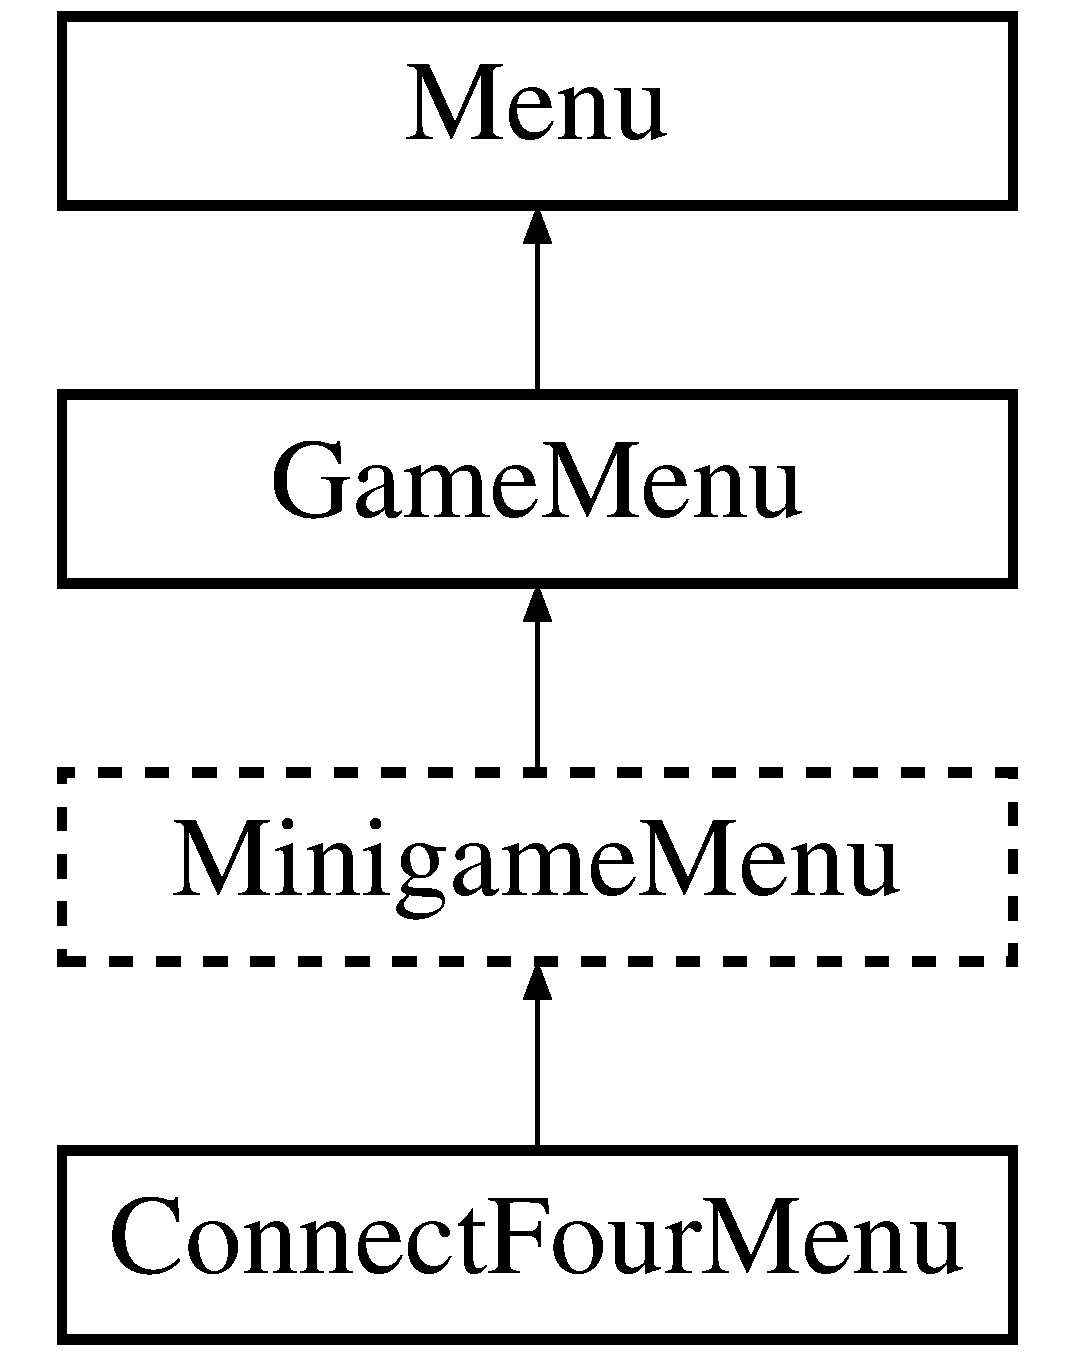
\includegraphics[height=4.000000cm]{classConnectFourMenu}
\end{center}
\end{figure}
\subsection*{Public Member Functions}
\begin{DoxyCompactItemize}
\item 
\hyperlink{classConnectFourMenu_a368513cbf367d7014e664667dbbb94ae}{Connect\-Four\-Menu} ()
\begin{DoxyCompactList}\small\item\em This is the default constructor. \end{DoxyCompactList}\item 
virtual \hyperlink{classConnectFourMenu_a53789934922dbbd5bfa5be90e69dfcb4}{$\sim$\-Connect\-Four\-Menu} ()
\begin{DoxyCompactList}\small\item\em This is the virtual destructor. \end{DoxyCompactList}\item 
virtual void \hyperlink{classConnectFourMenu_a6a826d0810795584cfb4b601d5cd5df2}{Set\-Options} (int row, int col, int space)
\item 
virtual void \hyperlink{classConnectFourMenu_a2af0c62dd776dd0e3d8c212f71eb3219}{Handle\-Input} (istream \&is)
\item 
int \hyperlink{classConnectFourMenu_a22ebfd1c6dac4040f023edd348191a0e}{Get\-Column} () const 
\begin{DoxyCompactList}\small\item\em Returns the chosen column. \end{DoxyCompactList}\end{DoxyCompactItemize}
\subsection*{Private Attributes}
\begin{DoxyCompactItemize}
\item 
int \hyperlink{classConnectFourMenu_ac45e28e0ff8b9b90295cd96da8459a47}{column}
\end{DoxyCompactItemize}
\subsection*{Additional Inherited Members}


\subsection{Detailed Description}
This is the menu class for the Connect Four minigame. 

\subsection{Constructor \& Destructor Documentation}
\hypertarget{classConnectFourMenu_a368513cbf367d7014e664667dbbb94ae}{\index{Connect\-Four\-Menu@{Connect\-Four\-Menu}!Connect\-Four\-Menu@{Connect\-Four\-Menu}}
\index{Connect\-Four\-Menu@{Connect\-Four\-Menu}!ConnectFourMenu@{Connect\-Four\-Menu}}
\subsubsection[{Connect\-Four\-Menu}]{\setlength{\rightskip}{0pt plus 5cm}Connect\-Four\-Menu\-::\-Connect\-Four\-Menu (
\begin{DoxyParamCaption}
{}
\end{DoxyParamCaption}
)}}\label{classConnectFourMenu_a368513cbf367d7014e664667dbbb94ae}


This is the default constructor. 

\begin{DoxyDate}{Date}
24/10/2017 
\end{DoxyDate}
\begin{DoxyAuthor}{Author}
Tomas Rigaux
\end{DoxyAuthor}
This is the implementationmenu class for the Connect Four minigame. \hypertarget{classConnectFourMenu_a53789934922dbbd5bfa5be90e69dfcb4}{\index{Connect\-Four\-Menu@{Connect\-Four\-Menu}!$\sim$\-Connect\-Four\-Menu@{$\sim$\-Connect\-Four\-Menu}}
\index{$\sim$\-Connect\-Four\-Menu@{$\sim$\-Connect\-Four\-Menu}!ConnectFourMenu@{Connect\-Four\-Menu}}
\subsubsection[{$\sim$\-Connect\-Four\-Menu}]{\setlength{\rightskip}{0pt plus 5cm}Connect\-Four\-Menu\-::$\sim$\-Connect\-Four\-Menu (
\begin{DoxyParamCaption}
{}
\end{DoxyParamCaption}
)\hspace{0.3cm}{\ttfamily [virtual]}}}\label{classConnectFourMenu_a53789934922dbbd5bfa5be90e69dfcb4}


This is the virtual destructor. 



\subsection{Member Function Documentation}
\hypertarget{classConnectFourMenu_a22ebfd1c6dac4040f023edd348191a0e}{\index{Connect\-Four\-Menu@{Connect\-Four\-Menu}!Get\-Column@{Get\-Column}}
\index{Get\-Column@{Get\-Column}!ConnectFourMenu@{Connect\-Four\-Menu}}
\subsubsection[{Get\-Column}]{\setlength{\rightskip}{0pt plus 5cm}int Connect\-Four\-Menu\-::\-Get\-Column (
\begin{DoxyParamCaption}
{}
\end{DoxyParamCaption}
) const\hspace{0.3cm}{\ttfamily [inline]}}}\label{classConnectFourMenu_a22ebfd1c6dac4040f023edd348191a0e}


Returns the chosen column. 

\hypertarget{classConnectFourMenu_a2af0c62dd776dd0e3d8c212f71eb3219}{\index{Connect\-Four\-Menu@{Connect\-Four\-Menu}!Handle\-Input@{Handle\-Input}}
\index{Handle\-Input@{Handle\-Input}!ConnectFourMenu@{Connect\-Four\-Menu}}
\subsubsection[{Handle\-Input}]{\setlength{\rightskip}{0pt plus 5cm}void Connect\-Four\-Menu\-::\-Handle\-Input (
\begin{DoxyParamCaption}
\item[{istream \&}]{is}
\end{DoxyParamCaption}
)\hspace{0.3cm}{\ttfamily [virtual]}}}\label{classConnectFourMenu_a2af0c62dd776dd0e3d8c212f71eb3219}
This function handles the input for the menu options. 
\begin{DoxyParams}[1]{Parameters}
\mbox{\tt in,out}  & {\em is} & The in-\/stream operator to read the input. \\
\hline
\end{DoxyParams}


Implements \hyperlink{classMinigameMenu_a3f854c4eefb0f3110cd085b3cfe56460}{Minigame\-Menu}.

\hypertarget{classConnectFourMenu_a6a826d0810795584cfb4b601d5cd5df2}{\index{Connect\-Four\-Menu@{Connect\-Four\-Menu}!Set\-Options@{Set\-Options}}
\index{Set\-Options@{Set\-Options}!ConnectFourMenu@{Connect\-Four\-Menu}}
\subsubsection[{Set\-Options}]{\setlength{\rightskip}{0pt plus 5cm}void Connect\-Four\-Menu\-::\-Set\-Options (
\begin{DoxyParamCaption}
\item[{int}]{row, }
\item[{int}]{col, }
\item[{int}]{space}
\end{DoxyParamCaption}
)\hspace{0.3cm}{\ttfamily [virtual]}}}\label{classConnectFourMenu_a6a826d0810795584cfb4b601d5cd5df2}
This function sets the specific options for the \hyperlink{classMenu}{Menu} type. 
\begin{DoxyParams}[1]{Parameters}
\mbox{\tt in}  & {\em row} & Determines which row the options will start being set at. \\
\hline
\mbox{\tt in}  & {\em col} & Determines which column the options will start from. \\
\hline
\mbox{\tt in}  & {\em How} & mush space inbetween rows. \\
\hline
\end{DoxyParams}


Implements \hyperlink{classMinigameMenu_abde3ae319bf1660a8626c6f765e054a8}{Minigame\-Menu}.



\subsection{Member Data Documentation}
\hypertarget{classConnectFourMenu_ac45e28e0ff8b9b90295cd96da8459a47}{\index{Connect\-Four\-Menu@{Connect\-Four\-Menu}!column@{column}}
\index{column@{column}!ConnectFourMenu@{Connect\-Four\-Menu}}
\subsubsection[{column}]{\setlength{\rightskip}{0pt plus 5cm}int Connect\-Four\-Menu\-::column\hspace{0.3cm}{\ttfamily [private]}}}\label{classConnectFourMenu_ac45e28e0ff8b9b90295cd96da8459a47}


The documentation for this class was generated from the following files\-:\begin{DoxyCompactItemize}
\item 
/home/rigt2720/\-Kodika/\-Menu/\hyperlink{ConnectFourMenu_8h}{Connect\-Four\-Menu.\-h}\item 
/home/rigt2720/\-Kodika/\-Menu/\hyperlink{ConnectFourMenu_8cpp}{Connect\-Four\-Menu.\-cpp}\end{DoxyCompactItemize}

\hypertarget{classConsumable}{\section{Consumable Class Reference}
\label{classConsumable}\index{Consumable@{Consumable}}
}


This class is an abstaract base class derived from \hyperlink{classItem}{Item} to represent in game consumables.  




{\ttfamily \#include $<$Consumable.\-h$>$}

Inheritance diagram for Consumable\-:\begin{figure}[H]
\begin{center}
\leavevmode
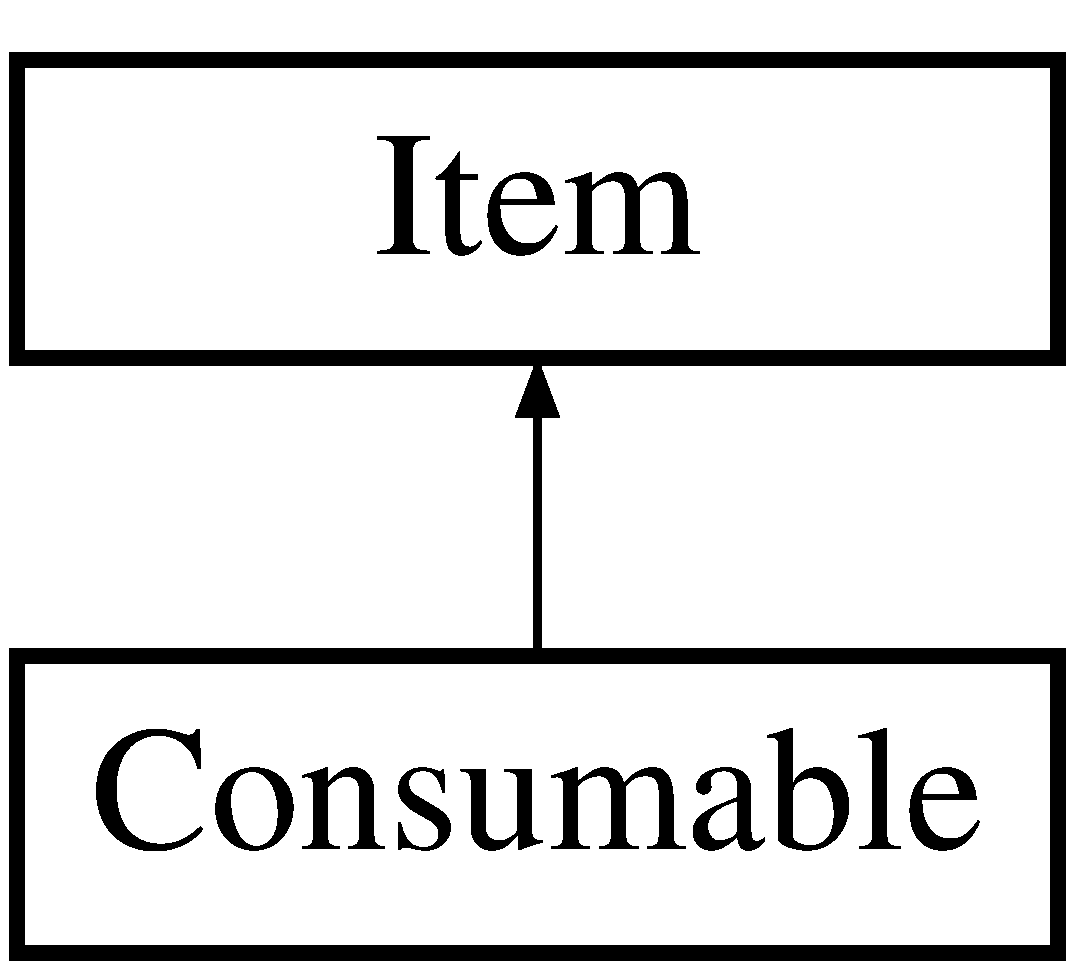
\includegraphics[height=3.000000cm]{classConsumable}
\end{center}
\end{figure}
\subsection*{Public Member Functions}
\begin{DoxyCompactItemize}
\item 
int \hyperlink{classConsumable_a043c6f13f4e3eb5121f2e8c85bf8b0da}{power} () const 
\item 
int \& \hyperlink{classConsumable_a1f0a7dee6c685c9b3d003d735877981b}{power} ()
\end{DoxyCompactItemize}
\subsection*{Protected Attributes}
\begin{DoxyCompactItemize}
\item 
int \hyperlink{classConsumable_a492024e0b8fd5b6c6e944116cbff3e32}{value}
\begin{DoxyCompactList}\small\item\em The actuall value of the item(ex how much health it restores) \end{DoxyCompactList}\item 
bool \hyperlink{classConsumable_a261f0f34c301027337ffe6bf32bf0200}{used}
\end{DoxyCompactItemize}
\subsection*{Additional Inherited Members}


\subsection{Detailed Description}
This class is an abstaract base class derived from \hyperlink{classItem}{Item} to represent in game consumables. 

\subsection{Member Function Documentation}
\hypertarget{classConsumable_a043c6f13f4e3eb5121f2e8c85bf8b0da}{\index{Consumable@{Consumable}!power@{power}}
\index{power@{power}!Consumable@{Consumable}}
\subsubsection[{power}]{\setlength{\rightskip}{0pt plus 5cm}int Consumable\-::power (
\begin{DoxyParamCaption}
{}
\end{DoxyParamCaption}
) const}}\label{classConsumable_a043c6f13f4e3eb5121f2e8c85bf8b0da}
Returns the the actuall value of the consumable (for reading only) \begin{DoxyReturn}{Returns}
value of the consumable 
\end{DoxyReturn}
\hypertarget{classConsumable_a1f0a7dee6c685c9b3d003d735877981b}{\index{Consumable@{Consumable}!power@{power}}
\index{power@{power}!Consumable@{Consumable}}
\subsubsection[{power}]{\setlength{\rightskip}{0pt plus 5cm}int\& Consumable\-::power (
\begin{DoxyParamCaption}
{}
\end{DoxyParamCaption}
)}}\label{classConsumable_a1f0a7dee6c685c9b3d003d735877981b}
Returns the the actuall value of the consumable (for writing) \begin{DoxyReturn}{Returns}
a reference to value 
\end{DoxyReturn}


\subsection{Member Data Documentation}
\hypertarget{classConsumable_a261f0f34c301027337ffe6bf32bf0200}{\index{Consumable@{Consumable}!used@{used}}
\index{used@{used}!Consumable@{Consumable}}
\subsubsection[{used}]{\setlength{\rightskip}{0pt plus 5cm}bool Consumable\-::used\hspace{0.3cm}{\ttfamily [protected]}}}\label{classConsumable_a261f0f34c301027337ffe6bf32bf0200}
\hypertarget{classConsumable_a492024e0b8fd5b6c6e944116cbff3e32}{\index{Consumable@{Consumable}!value@{value}}
\index{value@{value}!Consumable@{Consumable}}
\subsubsection[{value}]{\setlength{\rightskip}{0pt plus 5cm}int Consumable\-::value\hspace{0.3cm}{\ttfamily [protected]}}}\label{classConsumable_a492024e0b8fd5b6c6e944116cbff3e32}


The actuall value of the item(ex how much health it restores) 



The documentation for this class was generated from the following file\-:\begin{DoxyCompactItemize}
\item 
/home/rigt2720/\-Kodika/\-Item/\hyperlink{Consumable_8h}{Consumable.\-h}\end{DoxyCompactItemize}

\hypertarget{classDefaultImg}{\section{Default\-Img Class Reference}
\label{classDefaultImg}\index{Default\-Img@{Default\-Img}}
}


The \hyperlink{classDefaultImg}{Default\-Img} class represents a basic square image made of characters.  




{\ttfamily \#include $<$Default\-Img.\-h$>$}

Inheritance diagram for Default\-Img\-:\begin{figure}[H]
\begin{center}
\leavevmode
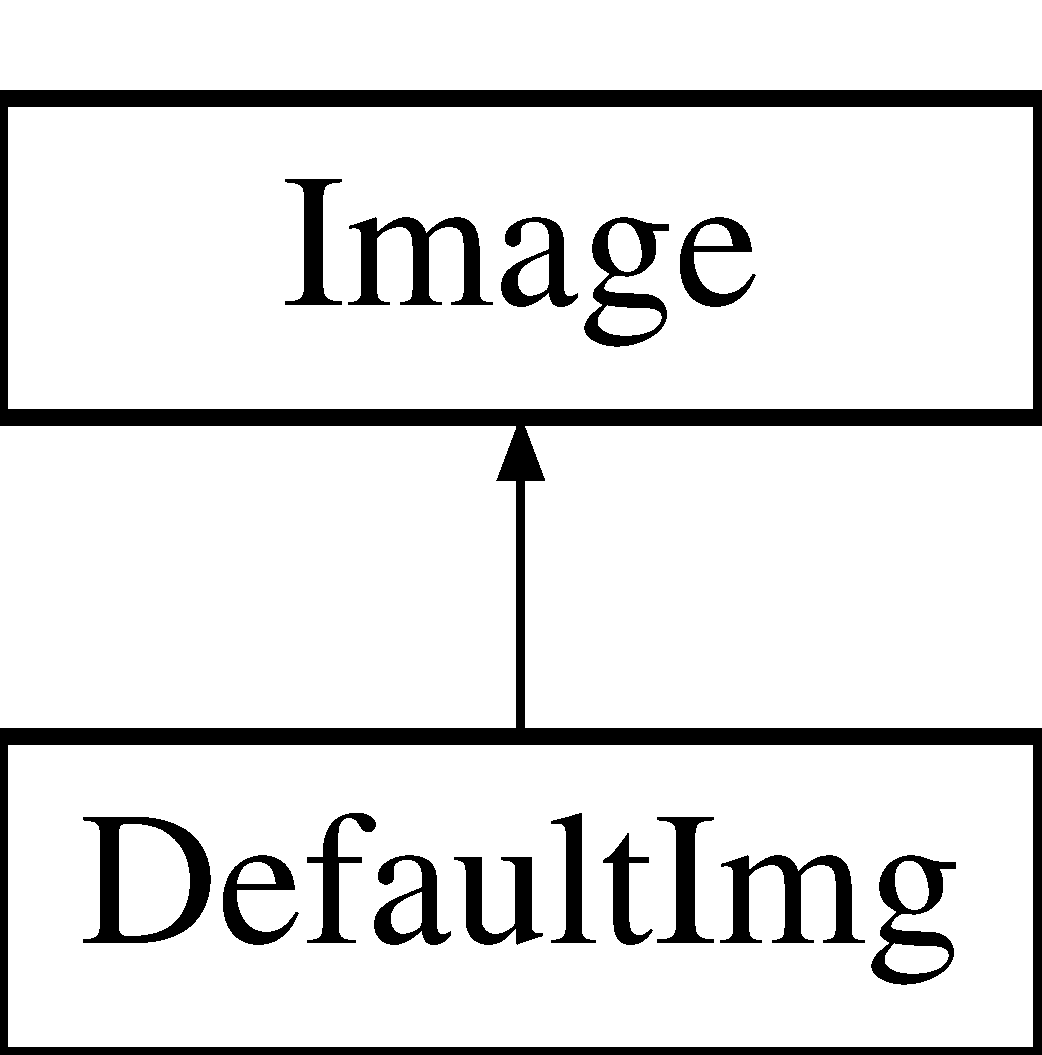
\includegraphics[height=2.000000cm]{classDefaultImg}
\end{center}
\end{figure}
\subsection*{Public Member Functions}
\begin{DoxyCompactItemize}
\item 
\hyperlink{classDefaultImg_a65e225ae4d43ce46b6661cb88dc5a9dc}{Default\-Img} (int h=3, int w=6, char c= '$\ast$')
\item 
\hyperlink{classDefaultImg_a98d6ecfaa4c02eba7b2c58ad0285521e}{Default\-Img} (const \hyperlink{classDefaultImg}{Default\-Img} \&img)
\item 
\hyperlink{classDefaultImg_ad4763b2a674e202d3ea99ceb179bad6a}{Default\-Img} (\hyperlink{classDefaultImg}{Default\-Img} \&img)
\item 
\hyperlink{classDefaultImg_ad3b823ee6222b08a4999802a0dc5ceec}{$\sim$\-Default\-Img} ()
\begin{DoxyCompactList}\small\item\em Destructor. \end{DoxyCompactList}\end{DoxyCompactItemize}
\subsection*{Private Member Functions}
\begin{DoxyCompactItemize}
\item 
void \hyperlink{classDefaultImg_a9ab21b397e0d23831b2944b651058b89}{Create} ()
\begin{DoxyCompactList}\small\item\em Function to create the image. \end{DoxyCompactList}\end{DoxyCompactItemize}
\subsection*{Private Attributes}
\begin{DoxyCompactItemize}
\item 
int \hyperlink{classDefaultImg_a563e191151451d5d3058ed646b8008ab}{\-\_\-height}
\begin{DoxyCompactList}\small\item\em The height of the image. \end{DoxyCompactList}\item 
int \hyperlink{classDefaultImg_a258f5ac708d83e06e924985dab85f221}{\-\_\-width}
\begin{DoxyCompactList}\small\item\em The width of the image. \end{DoxyCompactList}\item 
char \hyperlink{classDefaultImg_ac77e80e5517c44a6c6a7f7d50fe30bbc}{ch}
\begin{DoxyCompactList}\small\item\em The character used to draw the image. \end{DoxyCompactList}\end{DoxyCompactItemize}
\subsection*{Additional Inherited Members}


\subsection{Detailed Description}
The \hyperlink{classDefaultImg}{Default\-Img} class represents a basic square image made of characters. 

\begin{DoxyAuthor}{Author}
Reid Paulhus 
\end{DoxyAuthor}
\begin{DoxyDate}{Date}
Oct 20, 2017 
\end{DoxyDate}


\subsection{Constructor \& Destructor Documentation}
\hypertarget{classDefaultImg_a65e225ae4d43ce46b6661cb88dc5a9dc}{\index{Default\-Img@{Default\-Img}!Default\-Img@{Default\-Img}}
\index{Default\-Img@{Default\-Img}!DefaultImg@{Default\-Img}}
\subsubsection[{Default\-Img}]{\setlength{\rightskip}{0pt plus 5cm}Default\-Img\-::\-Default\-Img (
\begin{DoxyParamCaption}
\item[{int}]{h = {\ttfamily 3}, }
\item[{int}]{w = {\ttfamily 6}, }
\item[{char}]{c = {\ttfamily '$\ast$'}}
\end{DoxyParamCaption}
)}}\label{classDefaultImg_a65e225ae4d43ce46b6661cb88dc5a9dc}
Constructs an \hyperlink{classImage}{Image} object from the given dimensions 
\begin{DoxyParams}[1]{Parameters}
\mbox{\tt in}  & {\em h} & the height of the image, default to 3 \\
\hline
\mbox{\tt in}  & {\em w} & the width of the image, default to 6\\
\hline
\end{DoxyParams}
Default Constructor 
\begin{DoxyParams}[1]{Parameters}
\mbox{\tt in}  & {\em h} & the height of the image \\
\hline
\mbox{\tt in}  & {\em w} & the width of the image \\
\hline
\mbox{\tt in}  & {\em c} & the character used to draw the image \\
\hline
\end{DoxyParams}
\hypertarget{classDefaultImg_a98d6ecfaa4c02eba7b2c58ad0285521e}{\index{Default\-Img@{Default\-Img}!Default\-Img@{Default\-Img}}
\index{Default\-Img@{Default\-Img}!DefaultImg@{Default\-Img}}
\subsubsection[{Default\-Img}]{\setlength{\rightskip}{0pt plus 5cm}Default\-Img\-::\-Default\-Img (
\begin{DoxyParamCaption}
\item[{const {\bf Default\-Img} \&}]{image}
\end{DoxyParamCaption}
)}}\label{classDefaultImg_a98d6ecfaa4c02eba7b2c58ad0285521e}
Copy constructor duplicates a given picture 
\begin{DoxyParams}[1]{Parameters}
\mbox{\tt in}  & {\em img} & the image to copy from\\
\hline
\end{DoxyParams}
Copy constructor 
\begin{DoxyParams}[1]{Parameters}
\mbox{\tt in}  & {\em image} & the image copied from \\
\hline
\end{DoxyParams}
\hypertarget{classDefaultImg_ad4763b2a674e202d3ea99ceb179bad6a}{\index{Default\-Img@{Default\-Img}!Default\-Img@{Default\-Img}}
\index{Default\-Img@{Default\-Img}!DefaultImg@{Default\-Img}}
\subsubsection[{Default\-Img}]{\setlength{\rightskip}{0pt plus 5cm}Default\-Img\-::\-Default\-Img (
\begin{DoxyParamCaption}
\item[{{\bf Default\-Img} \&}]{image}
\end{DoxyParamCaption}
)}}\label{classDefaultImg_ad4763b2a674e202d3ea99ceb179bad6a}
Copy constructor duplicates a given picture 
\begin{DoxyParams}[1]{Parameters}
\mbox{\tt in}  & {\em img} & the image to copy from\\
\hline
\end{DoxyParams}
Copy constructor 
\begin{DoxyParams}[1]{Parameters}
\mbox{\tt in}  & {\em image} & the image copied from \\
\hline
\end{DoxyParams}
\hypertarget{classDefaultImg_ad3b823ee6222b08a4999802a0dc5ceec}{\index{Default\-Img@{Default\-Img}!$\sim$\-Default\-Img@{$\sim$\-Default\-Img}}
\index{$\sim$\-Default\-Img@{$\sim$\-Default\-Img}!DefaultImg@{Default\-Img}}
\subsubsection[{$\sim$\-Default\-Img}]{\setlength{\rightskip}{0pt plus 5cm}Default\-Img\-::$\sim$\-Default\-Img (
\begin{DoxyParamCaption}
{}
\end{DoxyParamCaption}
)}}\label{classDefaultImg_ad3b823ee6222b08a4999802a0dc5ceec}


Destructor. 



\subsection{Member Function Documentation}
\hypertarget{classDefaultImg_a9ab21b397e0d23831b2944b651058b89}{\index{Default\-Img@{Default\-Img}!Create@{Create}}
\index{Create@{Create}!DefaultImg@{Default\-Img}}
\subsubsection[{Create}]{\setlength{\rightskip}{0pt plus 5cm}void Default\-Img\-::\-Create (
\begin{DoxyParamCaption}
{}
\end{DoxyParamCaption}
)\hspace{0.3cm}{\ttfamily [private]}, {\ttfamily [virtual]}}}\label{classDefaultImg_a9ab21b397e0d23831b2944b651058b89}


Function to create the image. 

Function that creates the image by pushing back the vector. 

Reimplemented from \hyperlink{classImage_a6bb7dff9e4c4c31b2d63d7b0a330ef89}{Image}.



\subsection{Member Data Documentation}
\hypertarget{classDefaultImg_a563e191151451d5d3058ed646b8008ab}{\index{Default\-Img@{Default\-Img}!\-\_\-height@{\-\_\-height}}
\index{\-\_\-height@{\-\_\-height}!DefaultImg@{Default\-Img}}
\subsubsection[{\-\_\-height}]{\setlength{\rightskip}{0pt plus 5cm}int Default\-Img\-::\-\_\-height\hspace{0.3cm}{\ttfamily [private]}}}\label{classDefaultImg_a563e191151451d5d3058ed646b8008ab}


The height of the image. 

\hypertarget{classDefaultImg_a258f5ac708d83e06e924985dab85f221}{\index{Default\-Img@{Default\-Img}!\-\_\-width@{\-\_\-width}}
\index{\-\_\-width@{\-\_\-width}!DefaultImg@{Default\-Img}}
\subsubsection[{\-\_\-width}]{\setlength{\rightskip}{0pt plus 5cm}int Default\-Img\-::\-\_\-width\hspace{0.3cm}{\ttfamily [private]}}}\label{classDefaultImg_a258f5ac708d83e06e924985dab85f221}


The width of the image. 

\hypertarget{classDefaultImg_ac77e80e5517c44a6c6a7f7d50fe30bbc}{\index{Default\-Img@{Default\-Img}!ch@{ch}}
\index{ch@{ch}!DefaultImg@{Default\-Img}}
\subsubsection[{ch}]{\setlength{\rightskip}{0pt plus 5cm}char Default\-Img\-::ch\hspace{0.3cm}{\ttfamily [private]}}}\label{classDefaultImg_ac77e80e5517c44a6c6a7f7d50fe30bbc}


The character used to draw the image. 



The documentation for this class was generated from the following files\-:\begin{DoxyCompactItemize}
\item 
/home/rigt2720/\-Kodika/\-Image/\hyperlink{DefaultImg_8h}{Default\-Img.\-h}\item 
/home/rigt2720/\-Kodika/\-Image/\hyperlink{DefaultImg_8cpp}{Default\-Img.\-cpp}\end{DoxyCompactItemize}

\hypertarget{classDialogueMenu}{\section{Dialogue\-Menu Class Reference}
\label{classDialogueMenu}\index{Dialogue\-Menu@{Dialogue\-Menu}}
}


This is the menu displayed when the player character is engaging in dialogue with an N\-P\-C.  




{\ttfamily \#include $<$Dialogue\-Menu.\-h$>$}

Inheritance diagram for Dialogue\-Menu\-:\begin{figure}[H]
\begin{center}
\leavevmode
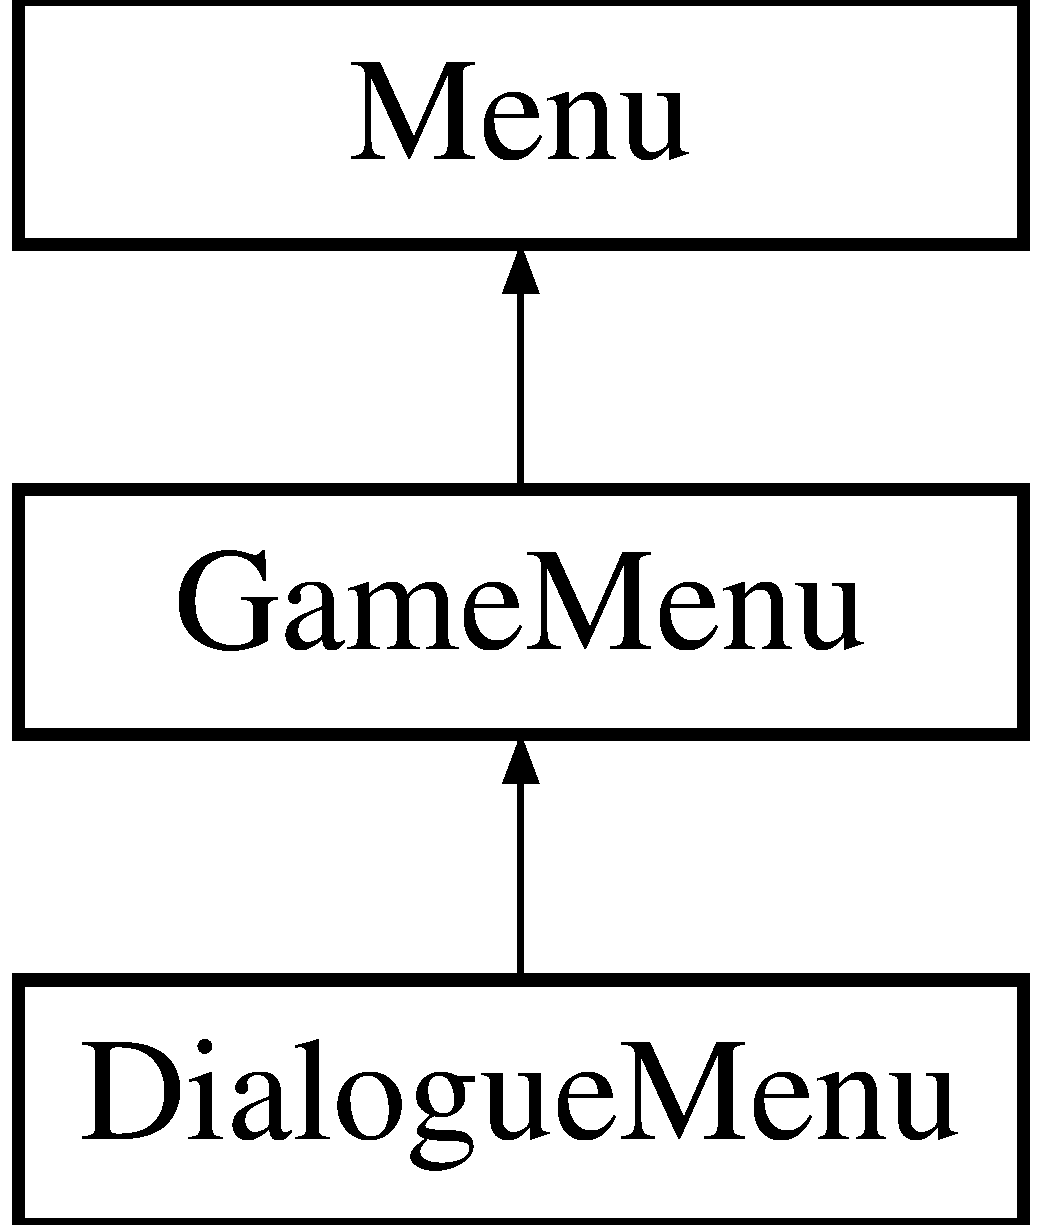
\includegraphics[height=3.000000cm]{classDialogueMenu}
\end{center}
\end{figure}
\subsection*{Public Member Functions}
\begin{DoxyCompactItemize}
\item 
\hypertarget{classDialogueMenu_a062e15c446d9a559a20bfdc19fb190c5}{\hyperlink{classDialogueMenu_a062e15c446d9a559a20bfdc19fb190c5}{Dialogue\-Menu} ()}\label{classDialogueMenu_a062e15c446d9a559a20bfdc19fb190c5}

\begin{DoxyCompactList}\small\item\em This is the default constructor. \end{DoxyCompactList}\item 
\hypertarget{classDialogueMenu_a11adf9b9db3cdeca6e0c38f0beec81dc}{virtual \hyperlink{classDialogueMenu_a11adf9b9db3cdeca6e0c38f0beec81dc}{$\sim$\-Dialogue\-Menu} ()}\label{classDialogueMenu_a11adf9b9db3cdeca6e0c38f0beec81dc}

\begin{DoxyCompactList}\small\item\em This is the virtual destructor. \end{DoxyCompactList}\item 
virtual void \hyperlink{classDialogueMenu_ac6ca871d2108cea94c33ef9f97d47cfd}{Set\-Options} (int row, int col)
\item 
virtual void \hyperlink{classDialogueMenu_af682f751ddb1f30c679a19dcf6703856}{Handle\-Input} (istream \&is)
\end{DoxyCompactItemize}
\subsection*{Additional Inherited Members}


\subsection{Detailed Description}
This is the menu displayed when the player character is engaging in dialogue with an N\-P\-C. 

\subsection{Member Function Documentation}
\hypertarget{classDialogueMenu_af682f751ddb1f30c679a19dcf6703856}{\index{Dialogue\-Menu@{Dialogue\-Menu}!Handle\-Input@{Handle\-Input}}
\index{Handle\-Input@{Handle\-Input}!DialogueMenu@{Dialogue\-Menu}}
\subsubsection[{Handle\-Input}]{\setlength{\rightskip}{0pt plus 5cm}void Dialogue\-Menu\-::\-Handle\-Input (
\begin{DoxyParamCaption}
\item[{istream \&}]{is}
\end{DoxyParamCaption}
)\hspace{0.3cm}{\ttfamily [virtual]}}}\label{classDialogueMenu_af682f751ddb1f30c679a19dcf6703856}
This function handles the input for the menu options. 
\begin{DoxyParams}[1]{Parameters}
\mbox{\tt in,out}  & {\em is} & The in-\/stream operator to read the input. \\
\hline
\end{DoxyParams}


Implements \hyperlink{classGameMenu_a02ba09feedece5773f44ba865ccffb42}{Game\-Menu}.

\hypertarget{classDialogueMenu_ac6ca871d2108cea94c33ef9f97d47cfd}{\index{Dialogue\-Menu@{Dialogue\-Menu}!Set\-Options@{Set\-Options}}
\index{Set\-Options@{Set\-Options}!DialogueMenu@{Dialogue\-Menu}}
\subsubsection[{Set\-Options}]{\setlength{\rightskip}{0pt plus 5cm}void Dialogue\-Menu\-::\-Set\-Options (
\begin{DoxyParamCaption}
\item[{int}]{row, }
\item[{int}]{col}
\end{DoxyParamCaption}
)\hspace{0.3cm}{\ttfamily [virtual]}}}\label{classDialogueMenu_ac6ca871d2108cea94c33ef9f97d47cfd}
This function sets the specific options for the \hyperlink{classMenu}{Menu} type. 
\begin{DoxyParams}[1]{Parameters}
\mbox{\tt in}  & {\em Options\-List} & A map of all the options for the current menu. Each option has a unique key to make input easier. \\
\hline
\mbox{\tt in}  & {\em type} & This denotes the type of menu to display. \\
\hline
\end{DoxyParams}


The documentation for this class was generated from the following files\-:\begin{DoxyCompactItemize}
\item 
Menu/Dialogue\-Menu.\-h\item 
Menu/Dialogue\-Menu.\-cpp\end{DoxyCompactItemize}

\hypertarget{classDialogueState}{\section{Dialogue\-State Class Reference}
\label{classDialogueState}\index{Dialogue\-State@{Dialogue\-State}}
}


This is the state of the game when the player character is engaged in dialogue with an N\-P\-C. Derived from \hyperlink{classGameState}{Game\-State}.  




{\ttfamily \#include $<$Dialogue\-State.\-h$>$}

Inheritance diagram for Dialogue\-State\-:\begin{figure}[H]
\begin{center}
\leavevmode
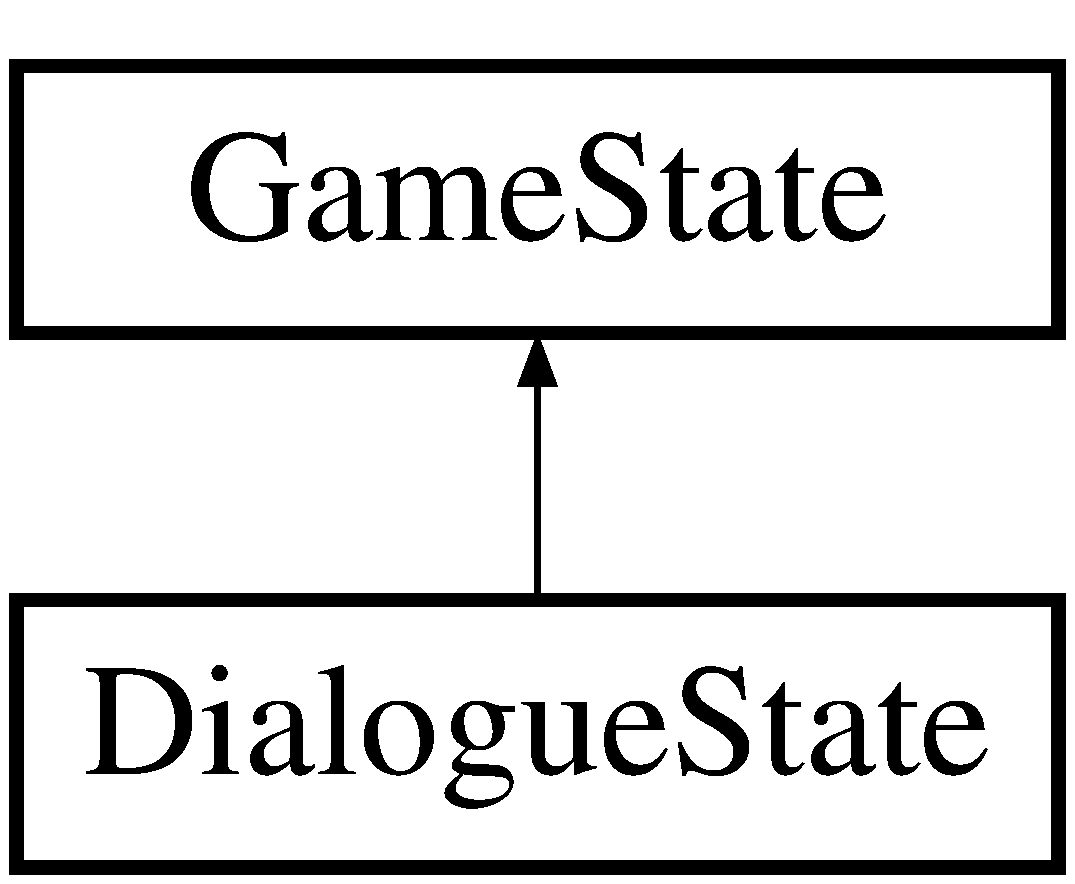
\includegraphics[height=2.000000cm]{classDialogueState}
\end{center}
\end{figure}
\subsection*{Public Member Functions}
\begin{DoxyCompactItemize}
\item 
\hypertarget{classDialogueState_a622d0916c1329a5e13675e4d7aff3b79}{\hyperlink{classDialogueState_a622d0916c1329a5e13675e4d7aff3b79}{Dialogue\-State} ()}\label{classDialogueState_a622d0916c1329a5e13675e4d7aff3b79}

\begin{DoxyCompactList}\small\item\em This is the default constructor. \end{DoxyCompactList}\item 
\hypertarget{classDialogueState_a203e463dc924a2492db74b749b81b9f1}{void \hyperlink{classDialogueState_a203e463dc924a2492db74b749b81b9f1}{Set} ()}\label{classDialogueState_a203e463dc924a2492db74b749b81b9f1}

\begin{DoxyCompactList}\small\item\em Sets the layout of the game. \end{DoxyCompactList}\item 
\hypertarget{classDialogueState_ab2f436b23d15e13cda1d756b8d47a982}{void \hyperlink{classDialogueState_ab2f436b23d15e13cda1d756b8d47a982}{Get} ()}\label{classDialogueState_ab2f436b23d15e13cda1d756b8d47a982}

\begin{DoxyCompactList}\small\item\em Gets the payout of the game. \end{DoxyCompactList}\end{DoxyCompactItemize}
\subsection*{Additional Inherited Members}


\subsection{Detailed Description}
This is the state of the game when the player character is engaged in dialogue with an N\-P\-C. Derived from \hyperlink{classGameState}{Game\-State}. 

The documentation for this class was generated from the following file\-:\begin{DoxyCompactItemize}
\item 
Game\-State/Dialogue\-State.\-h\end{DoxyCompactItemize}

\hypertarget{classExploreMenu}{\section{Explore\-Menu Class Reference}
\label{classExploreMenu}\index{Explore\-Menu@{Explore\-Menu}}
}


This is the menu displayed when the player character is being chosen before the game begins.  




{\ttfamily \#include $<$Explore\-Menu.\-h$>$}

Inheritance diagram for Explore\-Menu\-:\begin{figure}[H]
\begin{center}
\leavevmode
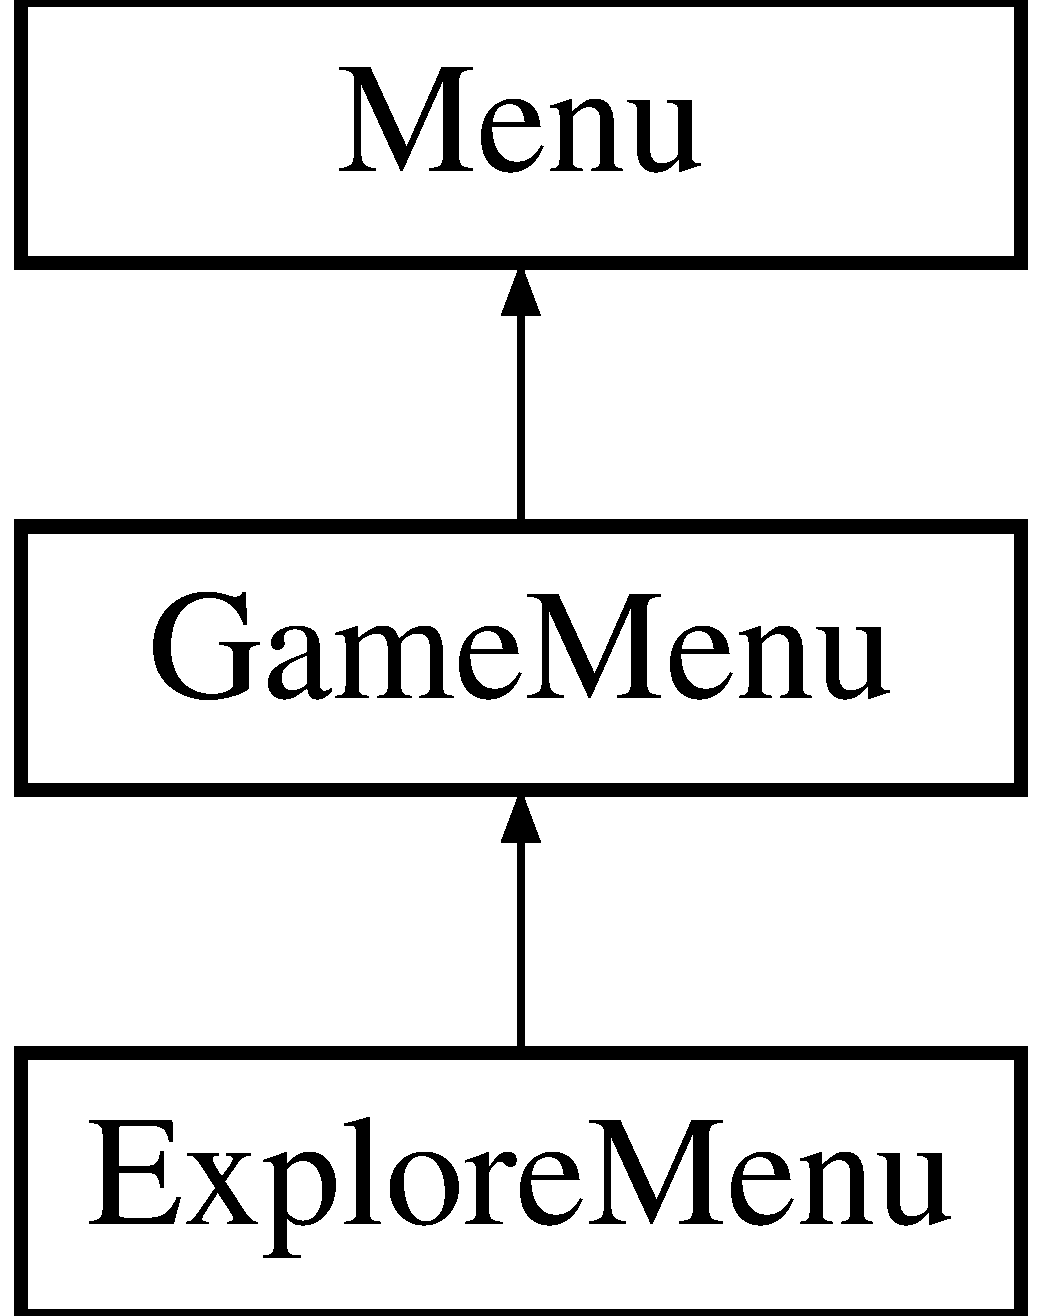
\includegraphics[height=3.000000cm]{classExploreMenu}
\end{center}
\end{figure}
\subsection*{Public Member Functions}
\begin{DoxyCompactItemize}
\item 
\hypertarget{classExploreMenu_ac05a4f8e2972f1617a702e04677f241b}{\hyperlink{classExploreMenu_ac05a4f8e2972f1617a702e04677f241b}{Explore\-Menu} ()}\label{classExploreMenu_ac05a4f8e2972f1617a702e04677f241b}

\begin{DoxyCompactList}\small\item\em This is the default constructor. \end{DoxyCompactList}\item 
\hypertarget{classExploreMenu_ade9d89c5b19679f01b73120120022e68}{virtual \hyperlink{classExploreMenu_ade9d89c5b19679f01b73120120022e68}{$\sim$\-Explore\-Menu} ()}\label{classExploreMenu_ade9d89c5b19679f01b73120120022e68}

\begin{DoxyCompactList}\small\item\em This is the virtual destructor. \end{DoxyCompactList}\item 
virtual void \hyperlink{classExploreMenu_ab31bbcb898e635120ec88eb296fa1825}{Set\-Options} (int row, int col)
\item 
virtual void \hyperlink{classExploreMenu_aa75a9fcba679d683855d3188f1fc3505}{Handle\-Input} (istream \&is)
\end{DoxyCompactItemize}
\subsection*{Additional Inherited Members}


\subsection{Detailed Description}
This is the menu displayed when the player character is being chosen before the game begins. 

This is the menu displayed when the player character is exploring rooms. 

\subsection{Member Function Documentation}
\hypertarget{classExploreMenu_aa75a9fcba679d683855d3188f1fc3505}{\index{Explore\-Menu@{Explore\-Menu}!Handle\-Input@{Handle\-Input}}
\index{Handle\-Input@{Handle\-Input}!ExploreMenu@{Explore\-Menu}}
\subsubsection[{Handle\-Input}]{\setlength{\rightskip}{0pt plus 5cm}void Explore\-Menu\-::\-Handle\-Input (
\begin{DoxyParamCaption}
\item[{istream \&}]{is}
\end{DoxyParamCaption}
)\hspace{0.3cm}{\ttfamily [virtual]}}}\label{classExploreMenu_aa75a9fcba679d683855d3188f1fc3505}
This function handles the input for the menu options. 
\begin{DoxyParams}[1]{Parameters}
\mbox{\tt in,out}  & {\em is} & The in-\/stream operator to read the input. \\
\hline
\end{DoxyParams}


Implements \hyperlink{classGameMenu_a02ba09feedece5773f44ba865ccffb42}{Game\-Menu}.

\hypertarget{classExploreMenu_ab31bbcb898e635120ec88eb296fa1825}{\index{Explore\-Menu@{Explore\-Menu}!Set\-Options@{Set\-Options}}
\index{Set\-Options@{Set\-Options}!ExploreMenu@{Explore\-Menu}}
\subsubsection[{Set\-Options}]{\setlength{\rightskip}{0pt plus 5cm}void Explore\-Menu\-::\-Set\-Options (
\begin{DoxyParamCaption}
\item[{int}]{row, }
\item[{int}]{col}
\end{DoxyParamCaption}
)\hspace{0.3cm}{\ttfamily [virtual]}}}\label{classExploreMenu_ab31bbcb898e635120ec88eb296fa1825}
This function sets the specific options for the \hyperlink{classMenu}{Menu} type. 
\begin{DoxyParams}[1]{Parameters}
\mbox{\tt in}  & {\em Options\-List} & A map of all the options for the current menu.\\
\hline
\mbox{\tt in}  & {\em type} & This denotes the type of menu to display. \\
\hline
\end{DoxyParams}


The documentation for this class was generated from the following files\-:\begin{DoxyCompactItemize}
\item 
Menu/Explore\-Menu.\-h\item 
Menu/Explore\-Menu.\-cpp\end{DoxyCompactItemize}

\hypertarget{classExploreState}{\section{Explore\-State Class Reference}
\label{classExploreState}\index{Explore\-State@{Explore\-State}}
}


This is defines the state of the game when the player character is exploring rooms. Derived from \hyperlink{classGameState}{Game\-State}.  




{\ttfamily \#include $<$Explore\-State.\-h$>$}

Inheritance diagram for Explore\-State\-:\begin{figure}[H]
\begin{center}
\leavevmode
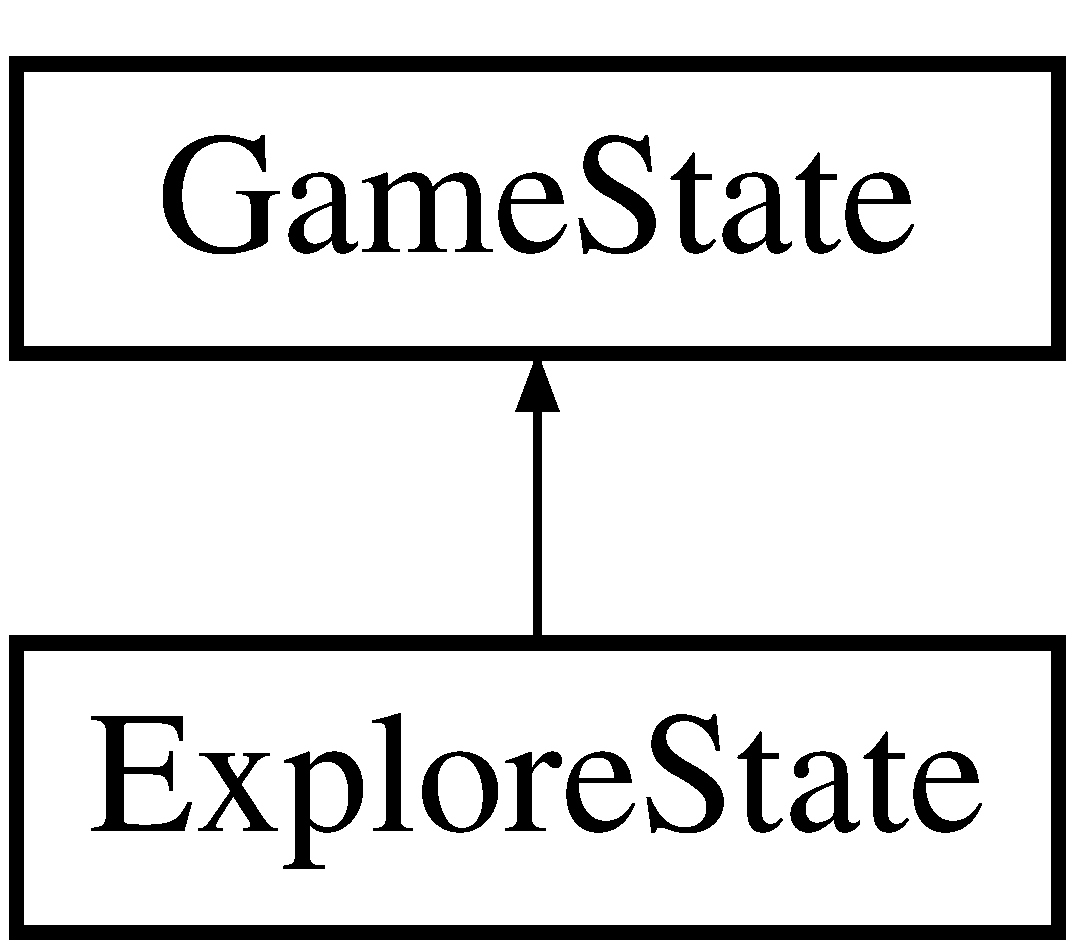
\includegraphics[height=2.000000cm]{classExploreState}
\end{center}
\end{figure}
\subsection*{Public Member Functions}
\begin{DoxyCompactItemize}
\item 
\hyperlink{classExploreState_ac10ad3cee219e8233a2c279392b70d52}{Explore\-State} ()
\begin{DoxyCompactList}\small\item\em This is the the default constructor. \end{DoxyCompactList}\item 
void \hyperlink{classExploreState_a8fb38f9fca513b87d914d077a0f2652b}{Set} ()
\begin{DoxyCompactList}\small\item\em Sets the layout for the game menu and screen. \end{DoxyCompactList}\item 
void \hyperlink{classExploreState_ace76d7a24bcb85f6f0a0fe0d0e763e21}{Get} ()
\begin{DoxyCompactList}\small\item\em Gets the layout for the game menu and screen. \end{DoxyCompactList}\end{DoxyCompactItemize}
\subsection*{Additional Inherited Members}


\subsection{Detailed Description}
This is defines the state of the game when the player character is exploring rooms. Derived from \hyperlink{classGameState}{Game\-State}. 

\begin{DoxyDate}{Date}
21/10/2017 
\end{DoxyDate}
\begin{DoxyAuthor}{Author}
Tomas Rigaux
\end{DoxyAuthor}
This is the state of the game when a player is exploring. 

\subsection{Constructor \& Destructor Documentation}
\hypertarget{classExploreState_ac10ad3cee219e8233a2c279392b70d52}{\index{Explore\-State@{Explore\-State}!Explore\-State@{Explore\-State}}
\index{Explore\-State@{Explore\-State}!ExploreState@{Explore\-State}}
\subsubsection[{Explore\-State}]{\setlength{\rightskip}{0pt plus 5cm}Explore\-State\-::\-Explore\-State (
\begin{DoxyParamCaption}
{}
\end{DoxyParamCaption}
)}}\label{classExploreState_ac10ad3cee219e8233a2c279392b70d52}


This is the the default constructor. 



\subsection{Member Function Documentation}
\hypertarget{classExploreState_ace76d7a24bcb85f6f0a0fe0d0e763e21}{\index{Explore\-State@{Explore\-State}!Get@{Get}}
\index{Get@{Get}!ExploreState@{Explore\-State}}
\subsubsection[{Get}]{\setlength{\rightskip}{0pt plus 5cm}void Explore\-State\-::\-Get (
\begin{DoxyParamCaption}
{}
\end{DoxyParamCaption}
)\hspace{0.3cm}{\ttfamily [virtual]}}}\label{classExploreState_ace76d7a24bcb85f6f0a0fe0d0e763e21}


Gets the layout for the game menu and screen. 



Implements \hyperlink{classGameState_a4283cb3aa5637d4815d64272843a0625}{Game\-State}.

\hypertarget{classExploreState_a8fb38f9fca513b87d914d077a0f2652b}{\index{Explore\-State@{Explore\-State}!Set@{Set}}
\index{Set@{Set}!ExploreState@{Explore\-State}}
\subsubsection[{Set}]{\setlength{\rightskip}{0pt plus 5cm}void Explore\-State\-::\-Set (
\begin{DoxyParamCaption}
{}
\end{DoxyParamCaption}
)\hspace{0.3cm}{\ttfamily [virtual]}}}\label{classExploreState_a8fb38f9fca513b87d914d077a0f2652b}


Sets the layout for the game menu and screen. 



Implements \hyperlink{classGameState_af22e9a43999f99b784a35fab85cd9208}{Game\-State}.



The documentation for this class was generated from the following file\-:\begin{DoxyCompactItemize}
\item 
/home/rigt2720/\-Kodika/\-Game\-State/\hyperlink{ExploreState_8h}{Explore\-State.\-h}\end{DoxyCompactItemize}

\hypertarget{classFightMenu}{\section{Fight\-Menu Class Reference}
\label{classFightMenu}\index{Fight\-Menu@{Fight\-Menu}}
}


This is the menu for the player to use when they are engaged in combat.  




{\ttfamily \#include $<$Fight\-Menu.\-h$>$}

Inheritance diagram for Fight\-Menu\-:\begin{figure}[H]
\begin{center}
\leavevmode
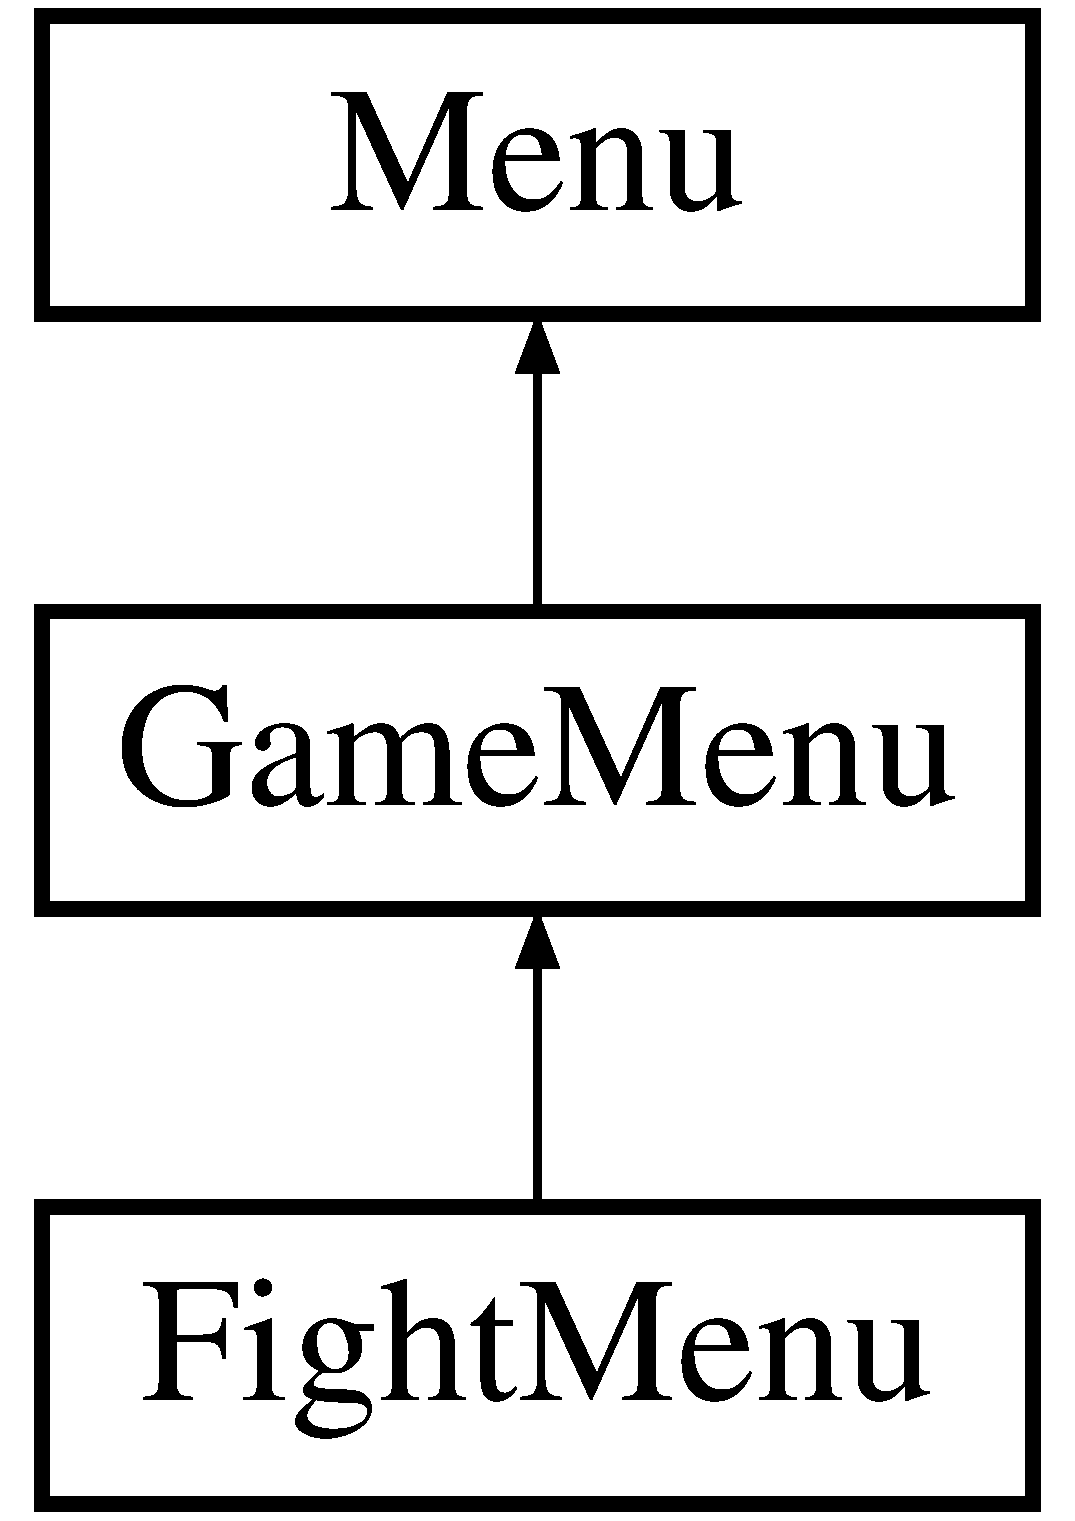
\includegraphics[height=3.000000cm]{classFightMenu}
\end{center}
\end{figure}
\subsection*{Public Member Functions}
\begin{DoxyCompactItemize}
\item 
\hyperlink{classFightMenu_a9f030d9a49e5b81dbaea8eab936cdf80}{Fight\-Menu} ()
\begin{DoxyCompactList}\small\item\em This is the default constructor. \end{DoxyCompactList}\item 
virtual \hyperlink{classFightMenu_a8a8792d7c674b0f19cdc9bf3a5ae96ca}{$\sim$\-Fight\-Menu} ()
\begin{DoxyCompactList}\small\item\em This is the virtual destructor. \end{DoxyCompactList}\item 
virtual void \hyperlink{classFightMenu_a234a915424eb00727d304834a4af352c}{Set\-Options} (int row=1, int col=1, int space=2)
\item 
virtual void \hyperlink{classFightMenu_a6d69cf9a19e7bae304d5a116285c1a51}{Handle\-Input} (istream \&is)
\end{DoxyCompactItemize}
\subsection*{Additional Inherited Members}


\subsection{Detailed Description}
This is the menu for the player to use when they are engaged in combat. 

\subsection{Constructor \& Destructor Documentation}
\hypertarget{classFightMenu_a9f030d9a49e5b81dbaea8eab936cdf80}{\index{Fight\-Menu@{Fight\-Menu}!Fight\-Menu@{Fight\-Menu}}
\index{Fight\-Menu@{Fight\-Menu}!FightMenu@{Fight\-Menu}}
\subsubsection[{Fight\-Menu}]{\setlength{\rightskip}{0pt plus 5cm}Fight\-Menu\-::\-Fight\-Menu (
\begin{DoxyParamCaption}
{}
\end{DoxyParamCaption}
)}}\label{classFightMenu_a9f030d9a49e5b81dbaea8eab936cdf80}


This is the default constructor. 

\begin{DoxyDate}{Date}
21/10/2017 
\end{DoxyDate}
\begin{DoxyAuthor}{Author}
Tomas Rigaux
\end{DoxyAuthor}
This is the fight class. This is the menu for the player to use when they are engaged in combat. \hypertarget{classFightMenu_a8a8792d7c674b0f19cdc9bf3a5ae96ca}{\index{Fight\-Menu@{Fight\-Menu}!$\sim$\-Fight\-Menu@{$\sim$\-Fight\-Menu}}
\index{$\sim$\-Fight\-Menu@{$\sim$\-Fight\-Menu}!FightMenu@{Fight\-Menu}}
\subsubsection[{$\sim$\-Fight\-Menu}]{\setlength{\rightskip}{0pt plus 5cm}Fight\-Menu\-::$\sim$\-Fight\-Menu (
\begin{DoxyParamCaption}
{}
\end{DoxyParamCaption}
)\hspace{0.3cm}{\ttfamily [virtual]}}}\label{classFightMenu_a8a8792d7c674b0f19cdc9bf3a5ae96ca}


This is the virtual destructor. 



\subsection{Member Function Documentation}
\hypertarget{classFightMenu_a6d69cf9a19e7bae304d5a116285c1a51}{\index{Fight\-Menu@{Fight\-Menu}!Handle\-Input@{Handle\-Input}}
\index{Handle\-Input@{Handle\-Input}!FightMenu@{Fight\-Menu}}
\subsubsection[{Handle\-Input}]{\setlength{\rightskip}{0pt plus 5cm}void Fight\-Menu\-::\-Handle\-Input (
\begin{DoxyParamCaption}
\item[{istream \&}]{is}
\end{DoxyParamCaption}
)\hspace{0.3cm}{\ttfamily [virtual]}}}\label{classFightMenu_a6d69cf9a19e7bae304d5a116285c1a51}
This function handles the input for the menu options. 
\begin{DoxyParams}[1]{Parameters}
\mbox{\tt in,out}  & {\em is} & The in-\/stream operator to read the input. \\
\hline
\end{DoxyParams}


Implements \hyperlink{classGameMenu_a02ba09feedece5773f44ba865ccffb42}{Game\-Menu}.

\hypertarget{classFightMenu_a234a915424eb00727d304834a4af352c}{\index{Fight\-Menu@{Fight\-Menu}!Set\-Options@{Set\-Options}}
\index{Set\-Options@{Set\-Options}!FightMenu@{Fight\-Menu}}
\subsubsection[{Set\-Options}]{\setlength{\rightskip}{0pt plus 5cm}void Fight\-Menu\-::\-Set\-Options (
\begin{DoxyParamCaption}
\item[{int}]{row = {\ttfamily 1}, }
\item[{int}]{col = {\ttfamily 1}, }
\item[{int}]{space = {\ttfamily 2}}
\end{DoxyParamCaption}
)\hspace{0.3cm}{\ttfamily [virtual]}}}\label{classFightMenu_a234a915424eb00727d304834a4af352c}
This function sets the specific options for the \hyperlink{classMenu}{Menu} type. 
\begin{DoxyParams}[1]{Parameters}
\mbox{\tt in}  & {\em row} & Determines which row the options will start being set at. \\
\hline
\mbox{\tt in}  & {\em col} & Determines which column the options will start from. \\
\hline
\mbox{\tt in}  & {\em How} & mush space inbetween rows. \\
\hline
\end{DoxyParams}


Implements \hyperlink{classGameMenu_ac32ff465c5a4f30979e8851fa21cb230}{Game\-Menu}.



The documentation for this class was generated from the following files\-:\begin{DoxyCompactItemize}
\item 
/home/rigt2720/\-Kodika/\-Menu/\hyperlink{FightMenu_8h}{Fight\-Menu.\-h}\item 
/home/rigt2720/\-Kodika/\-Menu/\hyperlink{FightMenu_8cpp}{Fight\-Menu.\-cpp}\end{DoxyCompactItemize}

\hypertarget{classFightState}{\section{Fight\-State Class Reference}
\label{classFightState}\index{Fight\-State@{Fight\-State}}
}


This is the state of the game when the player character is engaged in combat. Derived from \hyperlink{classGameState}{Game\-State}.  




{\ttfamily \#include $<$Fight\-State.\-h$>$}

Inheritance diagram for Fight\-State\-:\begin{figure}[H]
\begin{center}
\leavevmode
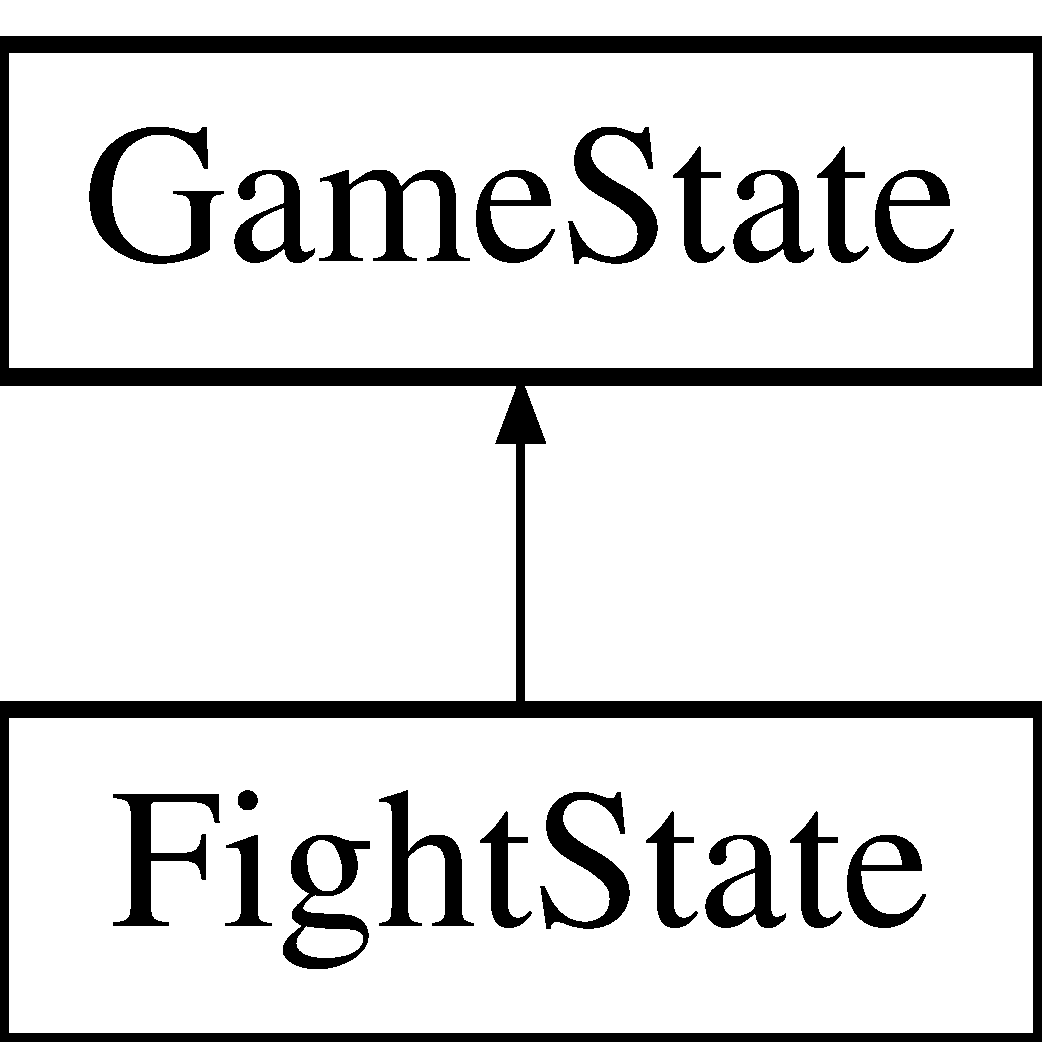
\includegraphics[height=2.000000cm]{classFightState}
\end{center}
\end{figure}
\subsection*{Public Member Functions}
\begin{DoxyCompactItemize}
\item 
\hyperlink{classFightState_ad63750cbcb525bf104bce58bc6c4e343}{Fight\-State} (\hyperlink{classPlayer}{Player} $\ast$p)
\begin{DoxyCompactList}\small\item\em This is the default constructor. \end{DoxyCompactList}\item 
void \hyperlink{classFightState_a853f6d2a9caf7343b8d75165e44bf5c1}{Set} ()
\begin{DoxyCompactList}\small\item\em Sets the layout of the game. \end{DoxyCompactList}\item 
void \hyperlink{classFightState_afeff88d0e0c0fa25049e2152190429ed}{Get} ()
\begin{DoxyCompactList}\small\item\em Outpouts the layout of the game. \end{DoxyCompactList}\end{DoxyCompactItemize}
\subsection*{Additional Inherited Members}


\subsection{Detailed Description}
This is the state of the game when the player character is engaged in combat. Derived from \hyperlink{classGameState}{Game\-State}. 

\begin{DoxyDate}{Date}
21/10/2017 
\end{DoxyDate}
\begin{DoxyAuthor}{Author}
Tomas Rigaux
\end{DoxyAuthor}
This is the state of the game when a player character is engaged in combat. 

\subsection{Constructor \& Destructor Documentation}
\hypertarget{classFightState_ad63750cbcb525bf104bce58bc6c4e343}{\index{Fight\-State@{Fight\-State}!Fight\-State@{Fight\-State}}
\index{Fight\-State@{Fight\-State}!FightState@{Fight\-State}}
\subsubsection[{Fight\-State}]{\setlength{\rightskip}{0pt plus 5cm}Fight\-State\-::\-Fight\-State (
\begin{DoxyParamCaption}
\item[{{\bf Player} $\ast$}]{p}
\end{DoxyParamCaption}
)}}\label{classFightState_ad63750cbcb525bf104bce58bc6c4e343}


This is the default constructor. 

\begin{DoxyDate}{Date}
25/11/2017 
\end{DoxyDate}
\begin{DoxyAuthor}{Author}
Tomas Rigaux
\end{DoxyAuthor}
This si the implementation for the F\-Ight State. 

\subsection{Member Function Documentation}
\hypertarget{classFightState_afeff88d0e0c0fa25049e2152190429ed}{\index{Fight\-State@{Fight\-State}!Get@{Get}}
\index{Get@{Get}!FightState@{Fight\-State}}
\subsubsection[{Get}]{\setlength{\rightskip}{0pt plus 5cm}void Fight\-State\-::\-Get (
\begin{DoxyParamCaption}
{}
\end{DoxyParamCaption}
)\hspace{0.3cm}{\ttfamily [virtual]}}}\label{classFightState_afeff88d0e0c0fa25049e2152190429ed}


Outpouts the layout of the game. 



Implements \hyperlink{classGameState_a4283cb3aa5637d4815d64272843a0625}{Game\-State}.

\hypertarget{classFightState_a853f6d2a9caf7343b8d75165e44bf5c1}{\index{Fight\-State@{Fight\-State}!Set@{Set}}
\index{Set@{Set}!FightState@{Fight\-State}}
\subsubsection[{Set}]{\setlength{\rightskip}{0pt plus 5cm}void Fight\-State\-::\-Set (
\begin{DoxyParamCaption}
{}
\end{DoxyParamCaption}
)\hspace{0.3cm}{\ttfamily [virtual]}}}\label{classFightState_a853f6d2a9caf7343b8d75165e44bf5c1}


Sets the layout of the game. 



Implements \hyperlink{classGameState_af22e9a43999f99b784a35fab85cd9208}{Game\-State}.



The documentation for this class was generated from the following files\-:\begin{DoxyCompactItemize}
\item 
/home/rigt2720/\-Kodika/\-Game\-State/\hyperlink{FightState_8h}{Fight\-State.\-h}\item 
/home/rigt2720/\-Kodika/\-Game\-State/\hyperlink{FightState_8cpp}{Fight\-State.\-cpp}\end{DoxyCompactItemize}

\hypertarget{classFood}{\section{Food Class Reference}
\label{classFood}\index{Food@{Food}}
}


Subclass of \hyperlink{classConsumable}{Consumable} to represent in game food.  




{\ttfamily \#include $<$My\-Consumables.\-h$>$}

Inheritance diagram for Food\-:\begin{figure}[H]
\begin{center}
\leavevmode
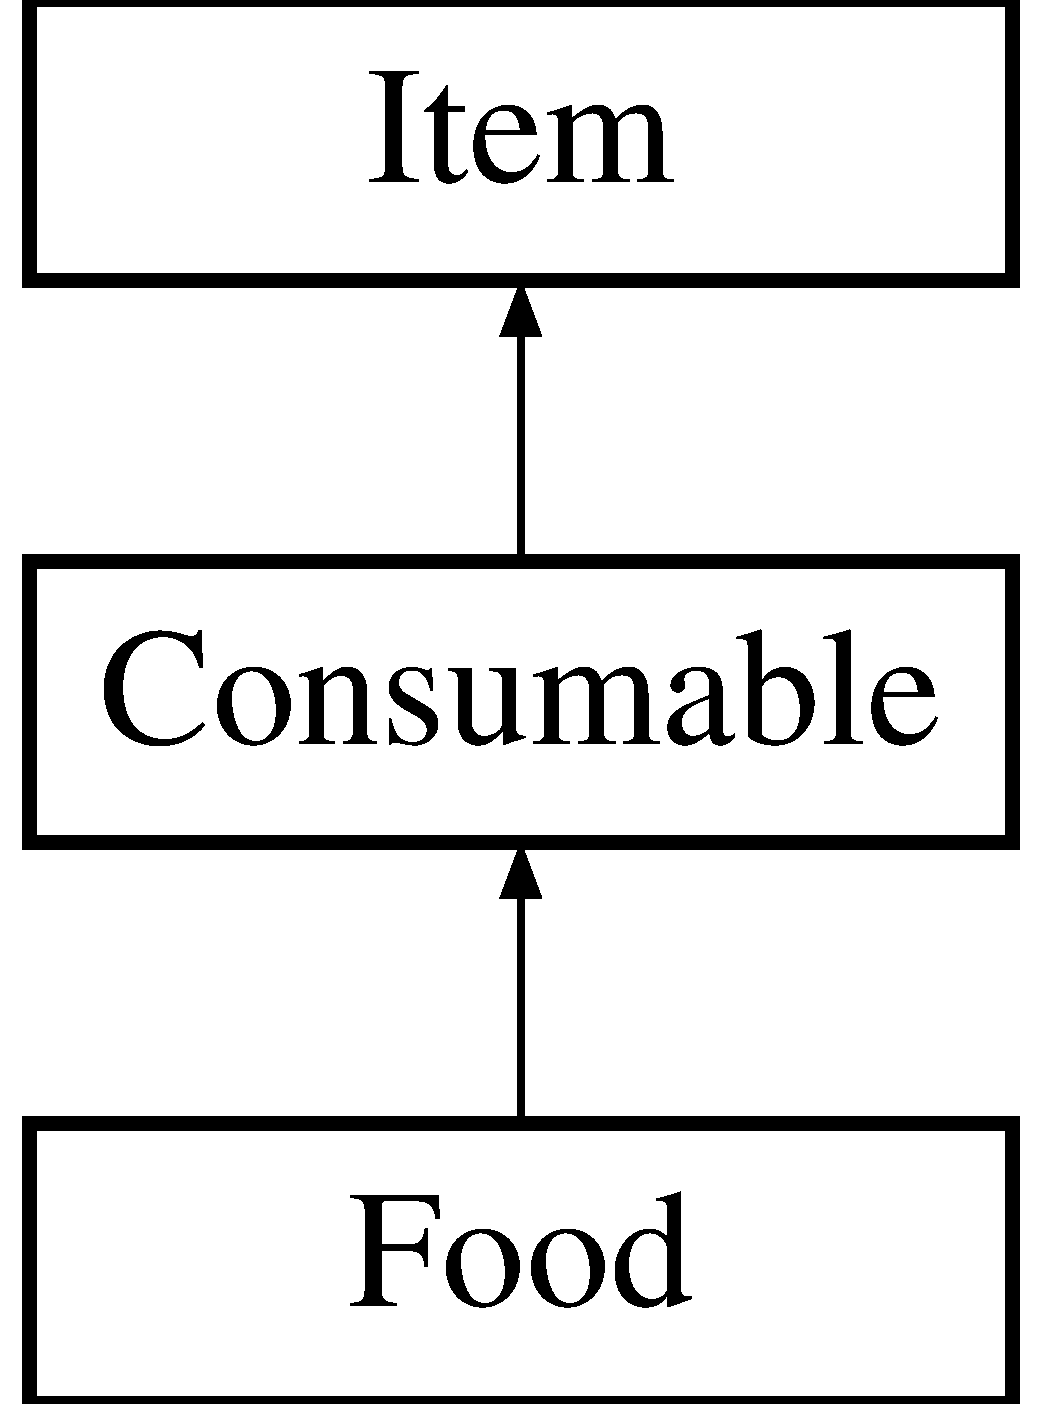
\includegraphics[height=3.000000cm]{classFood}
\end{center}
\end{figure}
\subsection*{Public Member Functions}
\begin{DoxyCompactItemize}
\item 
\hyperlink{classFood_a75d4d7f76fd495cc8133302ca9fdc485}{Food} ()
\begin{DoxyCompactList}\small\item\em \hyperlink{classFood}{Food} Constructor. \end{DoxyCompactList}\item 
bool \hyperlink{classFood_a03ce09da13a4d8b9bb7a789a3ede42be}{Use} (\hyperlink{classCharacter}{Character} $\ast$target)
\begin{DoxyCompactList}\small\item\em Use \hyperlink{classFood}{Food} Implementation. \end{DoxyCompactList}\end{DoxyCompactItemize}
\subsection*{Additional Inherited Members}


\subsection{Detailed Description}
Subclass of \hyperlink{classConsumable}{Consumable} to represent in game food. 

\subsection{Constructor \& Destructor Documentation}
\hypertarget{classFood_a75d4d7f76fd495cc8133302ca9fdc485}{\index{Food@{Food}!Food@{Food}}
\index{Food@{Food}!Food@{Food}}
\subsubsection[{Food}]{\setlength{\rightskip}{0pt plus 5cm}Food\-::\-Food (
\begin{DoxyParamCaption}
{}
\end{DoxyParamCaption}
)}}\label{classFood_a75d4d7f76fd495cc8133302ca9fdc485}


\hyperlink{classFood}{Food} Constructor. 

\hyperlink{classFood}{Food} Constuctor. 

\subsection{Member Function Documentation}
\hypertarget{classFood_a03ce09da13a4d8b9bb7a789a3ede42be}{\index{Food@{Food}!Use@{Use}}
\index{Use@{Use}!Food@{Food}}
\subsubsection[{Use}]{\setlength{\rightskip}{0pt plus 5cm}bool Food\-::\-Use (
\begin{DoxyParamCaption}
\item[{{\bf Character} $\ast$}]{target}
\end{DoxyParamCaption}
)\hspace{0.3cm}{\ttfamily [virtual]}}}\label{classFood_a03ce09da13a4d8b9bb7a789a3ede42be}


Use \hyperlink{classFood}{Food} Implementation. 

Defines what happens when the food is used 
\begin{DoxyParams}[1]{Parameters}
\mbox{\tt in}  & {\em target} & The \hyperlink{classCharacter}{Character} that the food is used on \\
\hline
\end{DoxyParams}
\begin{DoxyReturn}{Returns}
true if use was successfull  invalid\-\_\-argument Thrown if target is not a player 
\end{DoxyReturn}


Implements \hyperlink{classItem_abd3f52dd7fa25d497f2070e95d44ac03}{Item}.



The documentation for this class was generated from the following files\-:\begin{DoxyCompactItemize}
\item 
/home/rigt2720/\-Kodika/\-Item/\hyperlink{MyConsumables_8h}{My\-Consumables.\-h}\item 
/home/rigt2720/\-Kodika/\-Item/\hyperlink{MyConsumables_8cpp}{My\-Consumables.\-cpp}\end{DoxyCompactItemize}

\hypertarget{classGameMenu}{\section{Game\-Menu Class Reference}
\label{classGameMenu}\index{Game\-Menu@{Game\-Menu}}
}


An abstract class, this is the base class for the all the in-\/game menu classes. It requires less member functions than \hyperlink{classMenu}{Menu}.  




{\ttfamily \#include $<$Game\-Menu.\-h$>$}

Inheritance diagram for Game\-Menu\-:\begin{figure}[H]
\begin{center}
\leavevmode
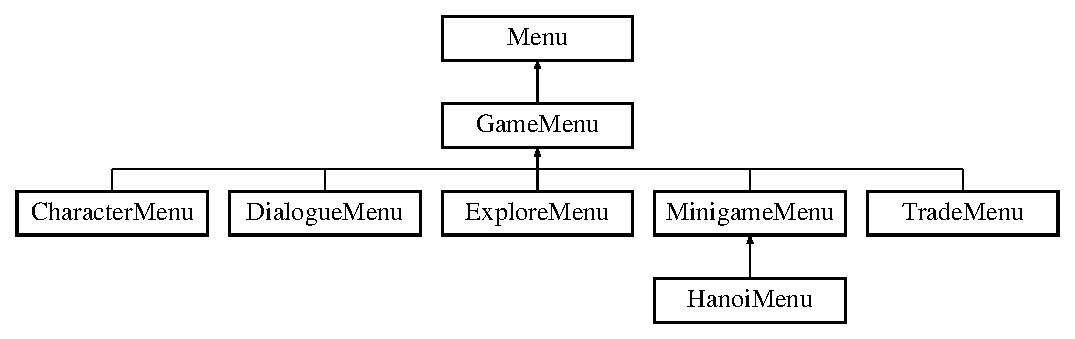
\includegraphics[height=4.000000cm]{classGameMenu}
\end{center}
\end{figure}
\subsection*{Public Member Functions}
\begin{DoxyCompactItemize}
\item 
\hypertarget{classGameMenu_ae31c50148abf655297a2a3eab53c15a3}{\hyperlink{classGameMenu_ae31c50148abf655297a2a3eab53c15a3}{Game\-Menu} ()}\label{classGameMenu_ae31c50148abf655297a2a3eab53c15a3}

\begin{DoxyCompactList}\small\item\em This is the default constructor. \end{DoxyCompactList}\item 
\hypertarget{classGameMenu_a8901f02e327b01a79b6e10a580154c44}{virtual \hyperlink{classGameMenu_a8901f02e327b01a79b6e10a580154c44}{$\sim$\-Game\-Menu} ()}\label{classGameMenu_a8901f02e327b01a79b6e10a580154c44}

\begin{DoxyCompactList}\small\item\em This is the virtual destructor. \end{DoxyCompactList}\item 
virtual void \hyperlink{classGameMenu_a25172d8d311df4f7b79074d60f74642e}{Set\-Options} (map$<$ string $>$ Options\-List, string type)=0
\item 
virtual void \hyperlink{classGameMenu_a02ba09feedece5773f44ba865ccffb42}{Handle\-Input} (istream \&is)=0
\end{DoxyCompactItemize}
\subsection*{Additional Inherited Members}


\subsection{Detailed Description}
An abstract class, this is the base class for the all the in-\/game menu classes. It requires less member functions than \hyperlink{classMenu}{Menu}. 

\subsection{Member Function Documentation}
\hypertarget{classGameMenu_a02ba09feedece5773f44ba865ccffb42}{\index{Game\-Menu@{Game\-Menu}!Handle\-Input@{Handle\-Input}}
\index{Handle\-Input@{Handle\-Input}!GameMenu@{Game\-Menu}}
\subsubsection[{Handle\-Input}]{\setlength{\rightskip}{0pt plus 5cm}virtual void Game\-Menu\-::\-Handle\-Input (
\begin{DoxyParamCaption}
\item[{istream \&}]{is}
\end{DoxyParamCaption}
)\hspace{0.3cm}{\ttfamily [pure virtual]}}}\label{classGameMenu_a02ba09feedece5773f44ba865ccffb42}
This function handles the input for the menu options. 
\begin{DoxyParams}[1]{Parameters}
\mbox{\tt in,out}  & {\em is} & The in-\/stream operator to read the input. \\
\hline
\end{DoxyParams}


Implemented in \hyperlink{classCharacterMenu_a7a9163eec7ac69aeb5431869a0675646}{Character\-Menu}, \hyperlink{classDialogueMenu_a2fa399f6e56c5421f161c0e90e17ac13}{Dialogue\-Menu}, \hyperlink{classExploreMenu_a6f057968d2aece06eef01b9da9b42c2d}{Explore\-Menu}, \hyperlink{classHanoiMenu_a8d287d810bc4cf49775503470830e48f}{Hanoi\-Menu}, \hyperlink{classMinigameMenu_a3f854c4eefb0f3110cd085b3cfe56460}{Minigame\-Menu}, and \hyperlink{classTradeMenu_a743dd5b1984d2640865ecd71d6e73d5e}{Trade\-Menu}.

\hypertarget{classGameMenu_a25172d8d311df4f7b79074d60f74642e}{\index{Game\-Menu@{Game\-Menu}!Set\-Options@{Set\-Options}}
\index{Set\-Options@{Set\-Options}!GameMenu@{Game\-Menu}}
\subsubsection[{Set\-Options}]{\setlength{\rightskip}{0pt plus 5cm}virtual void Game\-Menu\-::\-Set\-Options (
\begin{DoxyParamCaption}
\item[{map$<$ string $>$}]{Options\-List, }
\item[{string}]{type}
\end{DoxyParamCaption}
)\hspace{0.3cm}{\ttfamily [pure virtual]}}}\label{classGameMenu_a25172d8d311df4f7b79074d60f74642e}
This function sets the specific options for the \hyperlink{classMenu}{Menu} type. 
\begin{DoxyParams}[1]{Parameters}
\mbox{\tt in}  & {\em Options\-List} & A map of all the options for the current menu. Each option has a unique key to make input easier. \\
\hline
\mbox{\tt in}  & {\em type} & This denotes the type of menu to display. \\
\hline
\end{DoxyParams}


Implemented in \hyperlink{classCharacterMenu_a374493bc5b1e04b13647482c98df5fd6}{Character\-Menu}, \hyperlink{classDialogueMenu_ad9ce118b0515147fd59188e986cfbfee}{Dialogue\-Menu}, \hyperlink{classExploreMenu_a916408504bfc970370d199745f17b252}{Explore\-Menu}, \hyperlink{classHanoiMenu_a1ad3788638502865cb8d52040dcc27f8}{Hanoi\-Menu}, \hyperlink{classMinigameMenu_abf3dcda8c256be03ebe3661b8dde2ea2}{Minigame\-Menu}, and \hyperlink{classTradeMenu_a60cbb4e35a30cceab30448e19d13a882}{Trade\-Menu}.



The documentation for this class was generated from the following file\-:\begin{DoxyCompactItemize}
\item 
Menu/Game\-Menu.\-h\end{DoxyCompactItemize}

\hypertarget{classGameState}{\section{Game\-State Class Reference}
\label{classGameState}\index{Game\-State@{Game\-State}}
}


An abstract class, this class defines the state of the current 'state' of the game based on the current situation of the player character.  




{\ttfamily \#include $<$Game\-State.\-h$>$}

Inheritance diagram for Game\-State\-:\begin{figure}[H]
\begin{center}
\leavevmode
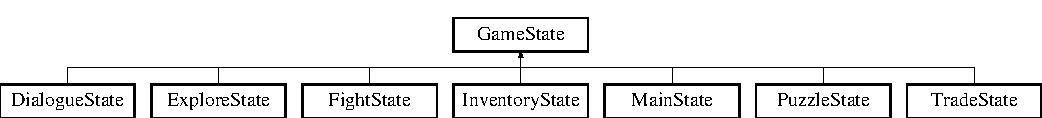
\includegraphics[height=1.584159cm]{classGameState}
\end{center}
\end{figure}
\subsection*{Public Member Functions}
\begin{DoxyCompactItemize}
\item 
\hyperlink{classGameState_a3d3d1f24fc9da8a9b2a1b081ac559c06}{Game\-State} (\hyperlink{classPlayer}{Player} $\ast$p=nullptr)
\begin{DoxyCompactList}\small\item\em Default constructor. \end{DoxyCompactList}\item 
virtual \hyperlink{classGameState_a517ef6eaba96896259fcefd0c66afc9e}{$\sim$\-Game\-State} ()
\begin{DoxyCompactList}\small\item\em Default destructor. \end{DoxyCompactList}\item 
virtual void \hyperlink{classGameState_af22e9a43999f99b784a35fab85cd9208}{Set} ()=0
\begin{DoxyCompactList}\small\item\em Sets the layout of the game. \end{DoxyCompactList}\item 
virtual void \hyperlink{classGameState_a4283cb3aa5637d4815d64272843a0625}{Get} ()=0
\begin{DoxyCompactList}\small\item\em Outputs the set layout. \end{DoxyCompactList}\item 
char \hyperlink{classGameState_a80d734fcbd886d8a0ce8e3191e770b3a}{Get\-State} () const 
\begin{DoxyCompactList}\small\item\em Returns the current state. \end{DoxyCompactList}\item 
\hyperlink{classPlayer}{Player} $\ast$ \hyperlink{classGameState_abcc93b8f1949ae4a39a5324b93d9291a}{Get\-Player} () const 
\begin{DoxyCompactList}\small\item\em Returns the current player. \end{DoxyCompactList}\item 
\hyperlink{classRoomTree}{Room\-Tree} $\ast$ \hyperlink{classGameState_a9659c39e354a27c0de9f09e27a05aa9d}{Get\-Room\-Tree} () const 
\begin{DoxyCompactList}\small\item\em Returns the room tree. \end{DoxyCompactList}\item 
\hyperlink{classMenu}{Menu} $\ast$ \hyperlink{classGameState_a55916672a315f362be7e17824fdaf3b4}{Get\-Menu} () const 
\begin{DoxyCompactList}\small\item\em Returns menu. \end{DoxyCompactList}\item 
\hyperlink{classScreen}{Screen} $\ast$ \hyperlink{classGameState_a275d26b431969575e7bd0de96be2d6b2}{Get\-Screen} () const 
\begin{DoxyCompactList}\small\item\em Returns the screen. \end{DoxyCompactList}\end{DoxyCompactItemize}
\subsection*{Protected Attributes}
\begin{DoxyCompactItemize}
\item 
\hyperlink{classMenu}{Menu} $\ast$ \hyperlink{classGameState_aebc12d6e90edfbe51a571858f6288f93}{menu}
\begin{DoxyCompactList}\small\item\em $<$ pointer to the menu. \end{DoxyCompactList}\item 
\hyperlink{classScreen}{Screen} $\ast$ \hyperlink{classGameState_a877c0c626d54802e54e876a56dc6603b}{screen}
\begin{DoxyCompactList}\small\item\em defines which gamestate will be used. \end{DoxyCompactList}\item 
char \hyperlink{classGameState_a541915faaaac7068797345cce53deb9c}{curr\-State}
\item 
\hyperlink{classRoomTree}{Room\-Tree} $\ast$ \hyperlink{classGameState_acf694139ba8388f8258eeffdb75f0c3b}{room\-Tree}
\begin{DoxyCompactList}\small\item\em allows access from different states to check whether room is complete \end{DoxyCompactList}\item 
\hyperlink{classPlayer}{Player} $\ast$ \hyperlink{classGameState_a580b319e1866f1bb79328c7d09581bdf}{player}
\end{DoxyCompactItemize}


\subsection{Detailed Description}
An abstract class, this class defines the state of the current 'state' of the game based on the current situation of the player character. 

\subsection{Constructor \& Destructor Documentation}
\hypertarget{classGameState_a3d3d1f24fc9da8a9b2a1b081ac559c06}{\index{Game\-State@{Game\-State}!Game\-State@{Game\-State}}
\index{Game\-State@{Game\-State}!GameState@{Game\-State}}
\subsubsection[{Game\-State}]{\setlength{\rightskip}{0pt plus 5cm}Game\-State\-::\-Game\-State (
\begin{DoxyParamCaption}
\item[{{\bf Player} $\ast$}]{p = {\ttfamily nullptr}}
\end{DoxyParamCaption}
)\hspace{0.3cm}{\ttfamily [inline]}}}\label{classGameState_a3d3d1f24fc9da8a9b2a1b081ac559c06}


Default constructor. 

\hypertarget{classGameState_a517ef6eaba96896259fcefd0c66afc9e}{\index{Game\-State@{Game\-State}!$\sim$\-Game\-State@{$\sim$\-Game\-State}}
\index{$\sim$\-Game\-State@{$\sim$\-Game\-State}!GameState@{Game\-State}}
\subsubsection[{$\sim$\-Game\-State}]{\setlength{\rightskip}{0pt plus 5cm}virtual Game\-State\-::$\sim$\-Game\-State (
\begin{DoxyParamCaption}
{}
\end{DoxyParamCaption}
)\hspace{0.3cm}{\ttfamily [inline]}, {\ttfamily [virtual]}}}\label{classGameState_a517ef6eaba96896259fcefd0c66afc9e}


Default destructor. 



\subsection{Member Function Documentation}
\hypertarget{classGameState_a4283cb3aa5637d4815d64272843a0625}{\index{Game\-State@{Game\-State}!Get@{Get}}
\index{Get@{Get}!GameState@{Game\-State}}
\subsubsection[{Get}]{\setlength{\rightskip}{0pt plus 5cm}virtual void Game\-State\-::\-Get (
\begin{DoxyParamCaption}
{}
\end{DoxyParamCaption}
)\hspace{0.3cm}{\ttfamily [pure virtual]}}}\label{classGameState_a4283cb3aa5637d4815d64272843a0625}


Outputs the set layout. 



Implemented in \hyperlink{classExploreState_ace76d7a24bcb85f6f0a0fe0d0e763e21}{Explore\-State}, \hyperlink{classInventoryState_a9358c4937e5bfe24017ac8985d56ed06}{Inventory\-State}, \hyperlink{classPuzzleState_ac9f6dd77d6471165d9eb2c18bd051dd1}{Puzzle\-State}, \hyperlink{classMainState_a23233e859905d025cfc031a12977a844}{Main\-State}, \hyperlink{classTradeState_a6479e704b1063281721200a0beac6bc1}{Trade\-State}, \hyperlink{classDialogueState_ab2f436b23d15e13cda1d756b8d47a982}{Dialogue\-State}, and \hyperlink{classFightState_afeff88d0e0c0fa25049e2152190429ed}{Fight\-State}.

\hypertarget{classGameState_a55916672a315f362be7e17824fdaf3b4}{\index{Game\-State@{Game\-State}!Get\-Menu@{Get\-Menu}}
\index{Get\-Menu@{Get\-Menu}!GameState@{Game\-State}}
\subsubsection[{Get\-Menu}]{\setlength{\rightskip}{0pt plus 5cm}{\bf Menu}$\ast$ Game\-State\-::\-Get\-Menu (
\begin{DoxyParamCaption}
{}
\end{DoxyParamCaption}
) const\hspace{0.3cm}{\ttfamily [inline]}}}\label{classGameState_a55916672a315f362be7e17824fdaf3b4}


Returns menu. 

\hypertarget{classGameState_abcc93b8f1949ae4a39a5324b93d9291a}{\index{Game\-State@{Game\-State}!Get\-Player@{Get\-Player}}
\index{Get\-Player@{Get\-Player}!GameState@{Game\-State}}
\subsubsection[{Get\-Player}]{\setlength{\rightskip}{0pt plus 5cm}{\bf Player}$\ast$ Game\-State\-::\-Get\-Player (
\begin{DoxyParamCaption}
{}
\end{DoxyParamCaption}
) const\hspace{0.3cm}{\ttfamily [inline]}}}\label{classGameState_abcc93b8f1949ae4a39a5324b93d9291a}


Returns the current player. 

\hypertarget{classGameState_a9659c39e354a27c0de9f09e27a05aa9d}{\index{Game\-State@{Game\-State}!Get\-Room\-Tree@{Get\-Room\-Tree}}
\index{Get\-Room\-Tree@{Get\-Room\-Tree}!GameState@{Game\-State}}
\subsubsection[{Get\-Room\-Tree}]{\setlength{\rightskip}{0pt plus 5cm}{\bf Room\-Tree}$\ast$ Game\-State\-::\-Get\-Room\-Tree (
\begin{DoxyParamCaption}
{}
\end{DoxyParamCaption}
) const\hspace{0.3cm}{\ttfamily [inline]}}}\label{classGameState_a9659c39e354a27c0de9f09e27a05aa9d}


Returns the room tree. 

\hypertarget{classGameState_a275d26b431969575e7bd0de96be2d6b2}{\index{Game\-State@{Game\-State}!Get\-Screen@{Get\-Screen}}
\index{Get\-Screen@{Get\-Screen}!GameState@{Game\-State}}
\subsubsection[{Get\-Screen}]{\setlength{\rightskip}{0pt plus 5cm}{\bf Screen}$\ast$ Game\-State\-::\-Get\-Screen (
\begin{DoxyParamCaption}
{}
\end{DoxyParamCaption}
) const\hspace{0.3cm}{\ttfamily [inline]}}}\label{classGameState_a275d26b431969575e7bd0de96be2d6b2}


Returns the screen. 

\hypertarget{classGameState_a80d734fcbd886d8a0ce8e3191e770b3a}{\index{Game\-State@{Game\-State}!Get\-State@{Get\-State}}
\index{Get\-State@{Get\-State}!GameState@{Game\-State}}
\subsubsection[{Get\-State}]{\setlength{\rightskip}{0pt plus 5cm}char Game\-State\-::\-Get\-State (
\begin{DoxyParamCaption}
{}
\end{DoxyParamCaption}
) const\hspace{0.3cm}{\ttfamily [inline]}}}\label{classGameState_a80d734fcbd886d8a0ce8e3191e770b3a}


Returns the current state. 

\hypertarget{classGameState_af22e9a43999f99b784a35fab85cd9208}{\index{Game\-State@{Game\-State}!Set@{Set}}
\index{Set@{Set}!GameState@{Game\-State}}
\subsubsection[{Set}]{\setlength{\rightskip}{0pt plus 5cm}virtual void Game\-State\-::\-Set (
\begin{DoxyParamCaption}
{}
\end{DoxyParamCaption}
)\hspace{0.3cm}{\ttfamily [pure virtual]}}}\label{classGameState_af22e9a43999f99b784a35fab85cd9208}


Sets the layout of the game. 



Implemented in \hyperlink{classExploreState_a8fb38f9fca513b87d914d077a0f2652b}{Explore\-State}, \hyperlink{classInventoryState_a47936e9d5683d344e87f3da176e97e4b}{Inventory\-State}, \hyperlink{classPuzzleState_a966b0f168ff5499f247c9ab519b524ab}{Puzzle\-State}, \hyperlink{classMainState_ac01eced9d617c8c8f5382a9aa96adb45}{Main\-State}, \hyperlink{classTradeState_af0d9fdcd649c1e74620dc77a4b8f92f9}{Trade\-State}, \hyperlink{classDialogueState_a203e463dc924a2492db74b749b81b9f1}{Dialogue\-State}, and \hyperlink{classFightState_a853f6d2a9caf7343b8d75165e44bf5c1}{Fight\-State}.



\subsection{Member Data Documentation}
\hypertarget{classGameState_a541915faaaac7068797345cce53deb9c}{\index{Game\-State@{Game\-State}!curr\-State@{curr\-State}}
\index{curr\-State@{curr\-State}!GameState@{Game\-State}}
\subsubsection[{curr\-State}]{\setlength{\rightskip}{0pt plus 5cm}char Game\-State\-::curr\-State\hspace{0.3cm}{\ttfamily [protected]}}}\label{classGameState_a541915faaaac7068797345cce53deb9c}
\hypertarget{classGameState_aebc12d6e90edfbe51a571858f6288f93}{\index{Game\-State@{Game\-State}!menu@{menu}}
\index{menu@{menu}!GameState@{Game\-State}}
\subsubsection[{menu}]{\setlength{\rightskip}{0pt plus 5cm}{\bf Menu}$\ast$ Game\-State\-::menu\hspace{0.3cm}{\ttfamily [protected]}}}\label{classGameState_aebc12d6e90edfbe51a571858f6288f93}


$<$ pointer to the menu. 

pointer to the screen; \hypertarget{classGameState_a580b319e1866f1bb79328c7d09581bdf}{\index{Game\-State@{Game\-State}!player@{player}}
\index{player@{player}!GameState@{Game\-State}}
\subsubsection[{player}]{\setlength{\rightskip}{0pt plus 5cm}{\bf Player}$\ast$ Game\-State\-::player\hspace{0.3cm}{\ttfamily [protected]}}}\label{classGameState_a580b319e1866f1bb79328c7d09581bdf}
\hypertarget{classGameState_acf694139ba8388f8258eeffdb75f0c3b}{\index{Game\-State@{Game\-State}!room\-Tree@{room\-Tree}}
\index{room\-Tree@{room\-Tree}!GameState@{Game\-State}}
\subsubsection[{room\-Tree}]{\setlength{\rightskip}{0pt plus 5cm}{\bf Room\-Tree}$\ast$ Game\-State\-::room\-Tree\hspace{0.3cm}{\ttfamily [protected]}}}\label{classGameState_acf694139ba8388f8258eeffdb75f0c3b}


allows access from different states to check whether room is complete 

\hypertarget{classGameState_a877c0c626d54802e54e876a56dc6603b}{\index{Game\-State@{Game\-State}!screen@{screen}}
\index{screen@{screen}!GameState@{Game\-State}}
\subsubsection[{screen}]{\setlength{\rightskip}{0pt plus 5cm}{\bf Screen}$\ast$ Game\-State\-::screen\hspace{0.3cm}{\ttfamily [protected]}}}\label{classGameState_a877c0c626d54802e54e876a56dc6603b}


defines which gamestate will be used. 



The documentation for this class was generated from the following file\-:\begin{DoxyCompactItemize}
\item 
/home/rigt2720/\-Kodika/\-Game\-State/\hyperlink{GameState_8h}{Game\-State.\-h}\end{DoxyCompactItemize}

\hypertarget{classHanoi}{\section{Hanoi Class Reference}
\label{classHanoi}\index{Hanoi@{Hanoi}}
}


This class contains the mini-\/game/\-Puzzle Towers of \hyperlink{classHanoi}{Hanoi}.  




{\ttfamily \#include $<$Hanoi.\-h$>$}

Inheritance diagram for Hanoi\-:\begin{figure}[H]
\begin{center}
\leavevmode
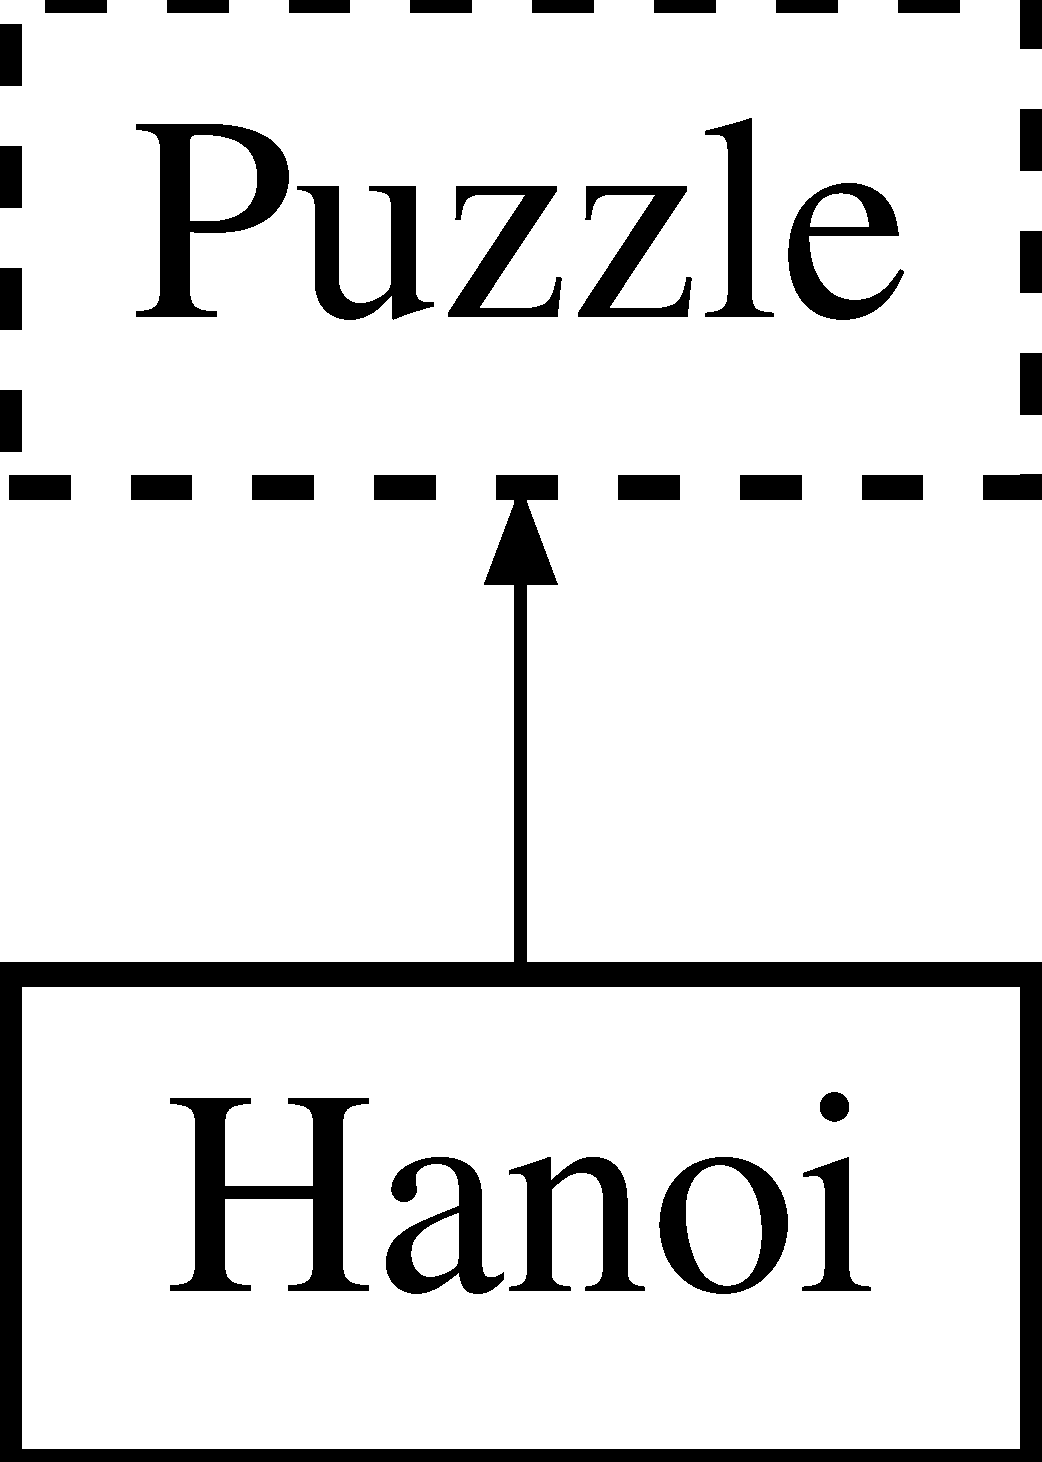
\includegraphics[height=2.000000cm]{classHanoi}
\end{center}
\end{figure}
\subsection*{Public Member Functions}
\begin{DoxyCompactItemize}
\item 
\hyperlink{classHanoi_a2af453ec21277f20edc002be08f22346}{Hanoi} ()
\begin{DoxyCompactList}\small\item\em Default constructor for hanoi, sets height to\-: and width to\-: \end{DoxyCompactList}\item 
\hyperlink{classHanoi_a59760291bfeda65330ff53c429a4e55b}{$\sim$\-Hanoi} ()
\begin{DoxyCompactList}\small\item\em Deconstructor. \end{DoxyCompactList}\item 
void \hyperlink{classHanoi_a2032169272e11d26ce253e2b264b9f31}{Run\-Game} ()
\end{DoxyCompactItemize}
\subsection*{Private Member Functions}
\begin{DoxyCompactItemize}
\item 
bool \hyperlink{classHanoi_a30dc9940db3589121396850f52ea7730}{Valid\-Move} (const int current\-Stack, const int new\-Stack) const 
\item 
void \hyperlink{classHanoi_a4dd4c6028ade2b265ce98e48c3f2fb2a}{Set\-Options\-In\-Menu} ()
\begin{DoxyCompactList}\small\item\em Sends the menu class the options for the player to select. \end{DoxyCompactList}\item 
void \hyperlink{classHanoi_aefbb40fc625506daa131076206e85b69}{Win\-Check} ()
\item 
void \hyperlink{classHanoi_a99b377a6ff0a2fc7d94d4fef0701345f}{Move\-Piece} (int user\-Selection)
\item 
int \hyperlink{classHanoi_a8ec34fb3a3682f6a8dcc1007e013ded0}{Which\-Disc\-From\-Size} (int size)
\item 
void \hyperlink{classHanoi_ad37d25d89cfdb3504d8f0702d0fff930}{Clear\-Screen\-Of\-Old\-Disc} (int size\-Of\-Disc, int target\-Tower, int y\-Coordinate)
\item 
void \hyperlink{classHanoi_a5dc7aab5bfe9d0b9d83ba75be22412e2}{Board\-Setup} ()
\end{DoxyCompactItemize}
\subsection*{Private Attributes}
\begin{DoxyCompactItemize}
\item 
std\-::vector$<$ stack$<$ \hyperlink{classDefaultImg}{Default\-Img} $>$ $>$ \hyperlink{classHanoi_afe67c656c8ce8c7006e8b7f23fbe9ae9}{tower}
\item 
int \hyperlink{classHanoi_abcdaa5a4b56f9c3916bf49e054e1cf8c}{number\-Of\-Stacks}
\item 
int \hyperlink{classHanoi_a826f3bc786cb5c7b6499508d0b8bc9b4}{max\-Stack\-Height}
\begin{DoxyCompactList}\small\item\em Maintains the height of the stacks in the game. \end{DoxyCompactList}\item 
bool \hyperlink{classHanoi_aff7a10d6c208cb15d315436b91017bed}{Game\-End}
\begin{DoxyCompactList}\small\item\em Used for the loop to see if the game has ended yet. \end{DoxyCompactList}\item 
\hyperlink{classScreen}{Screen} \hyperlink{classHanoi_a1b9bfd6a0428f772d78b66a5a3268c4c}{Hanoi\-Screen}
\begin{DoxyCompactList}\small\item\em Hanoi\-Screen stores and outputs the contents of the game to the terminal. \end{DoxyCompactList}\item 
\hyperlink{classHanoiMenu}{Hanoi\-Menu} \hyperlink{classHanoi_a7d73005d59c4f2134ffd564964ab3f49}{Hanoi\-Game\-Menu}
\begin{DoxyCompactList}\small\item\em \hyperlink{classGameMenu}{Game\-Menu} is used for handling input. \end{DoxyCompactList}\item 
std\-::vector$<$ \hyperlink{classDefaultImg}{Default\-Img} $>$ \hyperlink{classHanoi_a67a8288cd0c9a1acc3e5201621505afa}{discs\-Vector}
\item 
string \hyperlink{classHanoi_a9f971c51b287b61d8a919c26780e3f66}{menu\-Option1}
\begin{DoxyCompactList}\small\item\em Menu\-Option strings are used for outputting options to the user. \end{DoxyCompactList}\item 
string \hyperlink{classHanoi_ac9345e1760d1367ee05ecdf2e15d3d69}{menu\-Option2}
\item 
string \hyperlink{classHanoi_a94c22f2842c5473df08839fc9d4e860f}{menu\-Option3}
\item 
string \hyperlink{classHanoi_a3c6ac9ab6b2941ab955a2bc2c58cf93a}{menu\-Option4}
\end{DoxyCompactItemize}
\subsection*{Additional Inherited Members}


\subsection{Detailed Description}
This class contains the mini-\/game/\-Puzzle Towers of \hyperlink{classHanoi}{Hanoi}. 

\subsection{Constructor \& Destructor Documentation}
\hypertarget{classHanoi_a2af453ec21277f20edc002be08f22346}{\index{Hanoi@{Hanoi}!Hanoi@{Hanoi}}
\index{Hanoi@{Hanoi}!Hanoi@{Hanoi}}
\subsubsection[{Hanoi}]{\setlength{\rightskip}{0pt plus 5cm}Hanoi\-::\-Hanoi (
\begin{DoxyParamCaption}
{}
\end{DoxyParamCaption}
)}}\label{classHanoi_a2af453ec21277f20edc002be08f22346}


Default constructor for hanoi, sets height to\-: and width to\-: 

\begin{DoxyAuthor}{Author}
Tyler Siwy 
\end{DoxyAuthor}
\begin{DoxyDate}{Date}
Oct 20, 2017 
\end{DoxyDate}
Create default images for each of the disc to be drawn on the screen.

Put the discs into the first stack to start the game

Push the discs on in descending order since it's a stack.

Down one line for the next disc

Move two to left since the next disc is 4 chars larger. \hypertarget{classHanoi_a59760291bfeda65330ff53c429a4e55b}{\index{Hanoi@{Hanoi}!$\sim$\-Hanoi@{$\sim$\-Hanoi}}
\index{$\sim$\-Hanoi@{$\sim$\-Hanoi}!Hanoi@{Hanoi}}
\subsubsection[{$\sim$\-Hanoi}]{\setlength{\rightskip}{0pt plus 5cm}Hanoi\-::$\sim$\-Hanoi (
\begin{DoxyParamCaption}
{}
\end{DoxyParamCaption}
)}}\label{classHanoi_a59760291bfeda65330ff53c429a4e55b}


Deconstructor. 



\subsection{Member Function Documentation}
\hypertarget{classHanoi_a5dc7aab5bfe9d0b9d83ba75be22412e2}{\index{Hanoi@{Hanoi}!Board\-Setup@{Board\-Setup}}
\index{Board\-Setup@{Board\-Setup}!Hanoi@{Hanoi}}
\subsubsection[{Board\-Setup}]{\setlength{\rightskip}{0pt plus 5cm}void Hanoi\-::\-Board\-Setup (
\begin{DoxyParamCaption}
{}
\end{DoxyParamCaption}
)\hspace{0.3cm}{\ttfamily [private]}}}\label{classHanoi_a5dc7aab5bfe9d0b9d83ba75be22412e2}
\hypertarget{classHanoi_ad37d25d89cfdb3504d8f0702d0fff930}{\index{Hanoi@{Hanoi}!Clear\-Screen\-Of\-Old\-Disc@{Clear\-Screen\-Of\-Old\-Disc}}
\index{Clear\-Screen\-Of\-Old\-Disc@{Clear\-Screen\-Of\-Old\-Disc}!Hanoi@{Hanoi}}
\subsubsection[{Clear\-Screen\-Of\-Old\-Disc}]{\setlength{\rightskip}{0pt plus 5cm}void Hanoi\-::\-Clear\-Screen\-Of\-Old\-Disc (
\begin{DoxyParamCaption}
\item[{int}]{size\-Of\-Disc, }
\item[{int}]{target\-Tower, }
\item[{int}]{y\-Coordinate}
\end{DoxyParamCaption}
)\hspace{0.3cm}{\ttfamily [private]}}}\label{classHanoi_ad37d25d89cfdb3504d8f0702d0fff930}
Function which clears the discs previous location from the screen object You cannot use the erase function in the screen class because you would have to re-\/draw everything afterwards and the nature of a stack does not give you access to elements not on top. 18 is the center of the first tower, take away half the disc size to start in the right spot, add the interator as we move through the line.

18 is the center of the second tower, take away half the disc size to start in the right spot, add the interator as we move through the line.

84 is the center of the third tower, take away half the disc size to start in the right spot, add the interator as we move through the line. \hypertarget{classHanoi_a99b377a6ff0a2fc7d94d4fef0701345f}{\index{Hanoi@{Hanoi}!Move\-Piece@{Move\-Piece}}
\index{Move\-Piece@{Move\-Piece}!Hanoi@{Hanoi}}
\subsubsection[{Move\-Piece}]{\setlength{\rightskip}{0pt plus 5cm}void Hanoi\-::\-Move\-Piece (
\begin{DoxyParamCaption}
\item[{int}]{user\-Selection}
\end{DoxyParamCaption}
)\hspace{0.3cm}{\ttfamily [private]}}}\label{classHanoi_a99b377a6ff0a2fc7d94d4fef0701345f}
Moves the piece the depending on which option the player selects 
\begin{DoxyParams}[1]{Parameters}
\mbox{\tt in}  & {\em user\-Selection,the} & option of moves the player chose \\
\hline
\end{DoxyParams}
If the target tower is empty, the disc should go in spot 0, otherwise place it at the top.

Check if the move is a valid, if yes, move it over and pop it from its old location.

Push the right size disc from the vector of discs based on the size passed into Which\-Disc\-From\-Size, size is top\-Of\-Stack

If the target tower is empty, the disc should go in spot 0, otherwise place it at the top.

Check if the move is a valid, if yes, move it over and pop it from its old location.

If the target tower is empty, the disc should go in spot 0, otherwise place it at the top.

Check if the move is a valid, if yes, move it over and pop it from its old location.

If the tower is empty, the disc should go in spot 0, otherwise place it at the top.

Check if the move is a valid, if yes, move it over and pop it from its old location. \hypertarget{classHanoi_a2032169272e11d26ce253e2b264b9f31}{\index{Hanoi@{Hanoi}!Run\-Game@{Run\-Game}}
\index{Run\-Game@{Run\-Game}!Hanoi@{Hanoi}}
\subsubsection[{Run\-Game}]{\setlength{\rightskip}{0pt plus 5cm}void Hanoi\-::\-Run\-Game (
\begin{DoxyParamCaption}
{}
\end{DoxyParamCaption}
)\hspace{0.3cm}{\ttfamily [virtual]}}}\label{classHanoi_a2032169272e11d26ce253e2b264b9f31}
Method to run the game, serves as a 'main' for the mini-\/game, calling functions from private until the player has won. 

Implements \hyperlink{classPuzzle_ac92d0a3389cc806c0334aa224b72fa78}{Puzzle}.

\hypertarget{classHanoi_a4dd4c6028ade2b265ce98e48c3f2fb2a}{\index{Hanoi@{Hanoi}!Set\-Options\-In\-Menu@{Set\-Options\-In\-Menu}}
\index{Set\-Options\-In\-Menu@{Set\-Options\-In\-Menu}!Hanoi@{Hanoi}}
\subsubsection[{Set\-Options\-In\-Menu}]{\setlength{\rightskip}{0pt plus 5cm}void Hanoi\-::\-Set\-Options\-In\-Menu (
\begin{DoxyParamCaption}
{}
\end{DoxyParamCaption}
)\hspace{0.3cm}{\ttfamily [private]}, {\ttfamily [virtual]}}}\label{classHanoi_a4dd4c6028ade2b265ce98e48c3f2fb2a}


Sends the menu class the options for the player to select. 

Setup the options in the \hyperlink{classHanoiMenu}{Hanoi\-Menu} object. 

Implements \hyperlink{classPuzzle_adc90364342151caf536c4a34f2ca71d3}{Puzzle}.

\hypertarget{classHanoi_a30dc9940db3589121396850f52ea7730}{\index{Hanoi@{Hanoi}!Valid\-Move@{Valid\-Move}}
\index{Valid\-Move@{Valid\-Move}!Hanoi@{Hanoi}}
\subsubsection[{Valid\-Move}]{\setlength{\rightskip}{0pt plus 5cm}bool Hanoi\-::\-Valid\-Move (
\begin{DoxyParamCaption}
\item[{const int}]{current\-Stack, }
\item[{const int}]{new\-Stack}
\end{DoxyParamCaption}
) const\hspace{0.3cm}{\ttfamily [private]}}}\label{classHanoi_a30dc9940db3589121396850f52ea7730}
Checks the semantics of the user choice to make sure they aren't doing something that would break the game with their input. 
\begin{DoxyParams}[1]{Parameters}
\mbox{\tt in}  & {\em has} & been checked for syntax by input method \\
\hline
\end{DoxyParams}
If the disc on the current stack is smaller than the disc on the new stack it is considered a valid move, so return true, otherwise return false. \hypertarget{classHanoi_a8ec34fb3a3682f6a8dcc1007e013ded0}{\index{Hanoi@{Hanoi}!Which\-Disc\-From\-Size@{Which\-Disc\-From\-Size}}
\index{Which\-Disc\-From\-Size@{Which\-Disc\-From\-Size}!Hanoi@{Hanoi}}
\subsubsection[{Which\-Disc\-From\-Size}]{\setlength{\rightskip}{0pt plus 5cm}int Hanoi\-::\-Which\-Disc\-From\-Size (
\begin{DoxyParamCaption}
\item[{int}]{size}
\end{DoxyParamCaption}
)\hspace{0.3cm}{\ttfamily [private]}}}\label{classHanoi_a8ec34fb3a3682f6a8dcc1007e013ded0}
Which\-Disc\-From\-Size returns an index to wich disc in discs\-Vector the size is referenced with 
\begin{DoxyParams}[1]{Parameters}
\mbox{\tt in}  & {\em the} & size of disc we wouild like to know the location of \\
\hline
\end{DoxyParams}
\hypertarget{classHanoi_aefbb40fc625506daa131076206e85b69}{\index{Hanoi@{Hanoi}!Win\-Check@{Win\-Check}}
\index{Win\-Check@{Win\-Check}!Hanoi@{Hanoi}}
\subsubsection[{Win\-Check}]{\setlength{\rightskip}{0pt plus 5cm}void Hanoi\-::\-Win\-Check (
\begin{DoxyParamCaption}
{}
\end{DoxyParamCaption}
)\hspace{0.3cm}{\ttfamily [private]}}}\label{classHanoi_aefbb40fc625506daa131076206e85b69}
Checks the state of Tower to see if the player has won the game, sets Game\-End to true when they have completed the puzzle. If the user has managed to successfully move all discs to the last peg then its size should be 4. 

\subsection{Member Data Documentation}
\hypertarget{classHanoi_a67a8288cd0c9a1acc3e5201621505afa}{\index{Hanoi@{Hanoi}!discs\-Vector@{discs\-Vector}}
\index{discs\-Vector@{discs\-Vector}!Hanoi@{Hanoi}}
\subsubsection[{discs\-Vector}]{\setlength{\rightskip}{0pt plus 5cm}std\-::vector$<${\bf Default\-Img}$>$ Hanoi\-::discs\-Vector\hspace{0.3cm}{\ttfamily [private]}}}\label{classHanoi_a67a8288cd0c9a1acc3e5201621505afa}
A vector to store the size of all the discs in the game, stored in ascending order of size of discs. 0=3,1=7,2=11,3=15 \hypertarget{classHanoi_aff7a10d6c208cb15d315436b91017bed}{\index{Hanoi@{Hanoi}!Game\-End@{Game\-End}}
\index{Game\-End@{Game\-End}!Hanoi@{Hanoi}}
\subsubsection[{Game\-End}]{\setlength{\rightskip}{0pt plus 5cm}bool Hanoi\-::\-Game\-End\hspace{0.3cm}{\ttfamily [private]}}}\label{classHanoi_aff7a10d6c208cb15d315436b91017bed}


Used for the loop to see if the game has ended yet. 

\hypertarget{classHanoi_a7d73005d59c4f2134ffd564964ab3f49}{\index{Hanoi@{Hanoi}!Hanoi\-Game\-Menu@{Hanoi\-Game\-Menu}}
\index{Hanoi\-Game\-Menu@{Hanoi\-Game\-Menu}!Hanoi@{Hanoi}}
\subsubsection[{Hanoi\-Game\-Menu}]{\setlength{\rightskip}{0pt plus 5cm}{\bf Hanoi\-Menu} Hanoi\-::\-Hanoi\-Game\-Menu\hspace{0.3cm}{\ttfamily [private]}}}\label{classHanoi_a7d73005d59c4f2134ffd564964ab3f49}


\hyperlink{classGameMenu}{Game\-Menu} is used for handling input. 

\hypertarget{classHanoi_a1b9bfd6a0428f772d78b66a5a3268c4c}{\index{Hanoi@{Hanoi}!Hanoi\-Screen@{Hanoi\-Screen}}
\index{Hanoi\-Screen@{Hanoi\-Screen}!Hanoi@{Hanoi}}
\subsubsection[{Hanoi\-Screen}]{\setlength{\rightskip}{0pt plus 5cm}{\bf Screen} Hanoi\-::\-Hanoi\-Screen\hspace{0.3cm}{\ttfamily [private]}}}\label{classHanoi_a1b9bfd6a0428f772d78b66a5a3268c4c}


Hanoi\-Screen stores and outputs the contents of the game to the terminal. 

\hypertarget{classHanoi_a826f3bc786cb5c7b6499508d0b8bc9b4}{\index{Hanoi@{Hanoi}!max\-Stack\-Height@{max\-Stack\-Height}}
\index{max\-Stack\-Height@{max\-Stack\-Height}!Hanoi@{Hanoi}}
\subsubsection[{max\-Stack\-Height}]{\setlength{\rightskip}{0pt plus 5cm}int Hanoi\-::max\-Stack\-Height\hspace{0.3cm}{\ttfamily [private]}}}\label{classHanoi_a826f3bc786cb5c7b6499508d0b8bc9b4}


Maintains the height of the stacks in the game. 

\hypertarget{classHanoi_a9f971c51b287b61d8a919c26780e3f66}{\index{Hanoi@{Hanoi}!menu\-Option1@{menu\-Option1}}
\index{menu\-Option1@{menu\-Option1}!Hanoi@{Hanoi}}
\subsubsection[{menu\-Option1}]{\setlength{\rightskip}{0pt plus 5cm}string Hanoi\-::menu\-Option1\hspace{0.3cm}{\ttfamily [private]}}}\label{classHanoi_a9f971c51b287b61d8a919c26780e3f66}


Menu\-Option strings are used for outputting options to the user. 

\hypertarget{classHanoi_ac9345e1760d1367ee05ecdf2e15d3d69}{\index{Hanoi@{Hanoi}!menu\-Option2@{menu\-Option2}}
\index{menu\-Option2@{menu\-Option2}!Hanoi@{Hanoi}}
\subsubsection[{menu\-Option2}]{\setlength{\rightskip}{0pt plus 5cm}string Hanoi\-::menu\-Option2\hspace{0.3cm}{\ttfamily [private]}}}\label{classHanoi_ac9345e1760d1367ee05ecdf2e15d3d69}
\hypertarget{classHanoi_a94c22f2842c5473df08839fc9d4e860f}{\index{Hanoi@{Hanoi}!menu\-Option3@{menu\-Option3}}
\index{menu\-Option3@{menu\-Option3}!Hanoi@{Hanoi}}
\subsubsection[{menu\-Option3}]{\setlength{\rightskip}{0pt plus 5cm}string Hanoi\-::menu\-Option3\hspace{0.3cm}{\ttfamily [private]}}}\label{classHanoi_a94c22f2842c5473df08839fc9d4e860f}
\hypertarget{classHanoi_a3c6ac9ab6b2941ab955a2bc2c58cf93a}{\index{Hanoi@{Hanoi}!menu\-Option4@{menu\-Option4}}
\index{menu\-Option4@{menu\-Option4}!Hanoi@{Hanoi}}
\subsubsection[{menu\-Option4}]{\setlength{\rightskip}{0pt plus 5cm}string Hanoi\-::menu\-Option4\hspace{0.3cm}{\ttfamily [private]}}}\label{classHanoi_a3c6ac9ab6b2941ab955a2bc2c58cf93a}
\hypertarget{classHanoi_abcdaa5a4b56f9c3916bf49e054e1cf8c}{\index{Hanoi@{Hanoi}!number\-Of\-Stacks@{number\-Of\-Stacks}}
\index{number\-Of\-Stacks@{number\-Of\-Stacks}!Hanoi@{Hanoi}}
\subsubsection[{number\-Of\-Stacks}]{\setlength{\rightskip}{0pt plus 5cm}int Hanoi\-::number\-Of\-Stacks\hspace{0.3cm}{\ttfamily [private]}}}\label{classHanoi_abcdaa5a4b56f9c3916bf49e054e1cf8c}
Number of stacks in the game X-\/coordinate size in the tower vector \hypertarget{classHanoi_afe67c656c8ce8c7006e8b7f23fbe9ae9}{\index{Hanoi@{Hanoi}!tower@{tower}}
\index{tower@{tower}!Hanoi@{Hanoi}}
\subsubsection[{tower}]{\setlength{\rightskip}{0pt plus 5cm}std\-::vector$<$stack$<${\bf Default\-Img}$>$ $>$ Hanoi\-::tower\hspace{0.3cm}{\ttfamily [private]}}}\label{classHanoi_afe67c656c8ce8c7006e8b7f23fbe9ae9}
The vector which holds each towers' contents. Contents are stored as integers. 

The documentation for this class was generated from the following files\-:\begin{DoxyCompactItemize}
\item 
/home/rigt2720/\-Kodika/\-Puzzles/\hyperlink{Hanoi_8h}{Hanoi.\-h}\item 
/home/rigt2720/\-Kodika/\-Puzzles/\hyperlink{Hanoi_8cpp}{Hanoi.\-cpp}\end{DoxyCompactItemize}

\hypertarget{classHanoiMenu}{\section{Hanoi\-Menu Class Reference}
\label{classHanoiMenu}\index{Hanoi\-Menu@{Hanoi\-Menu}}
}


This is the menu class for the \hyperlink{classHanoi}{Hanoi} minigame.  


Inheritance diagram for Hanoi\-Menu\-:\begin{figure}[H]
\begin{center}
\leavevmode
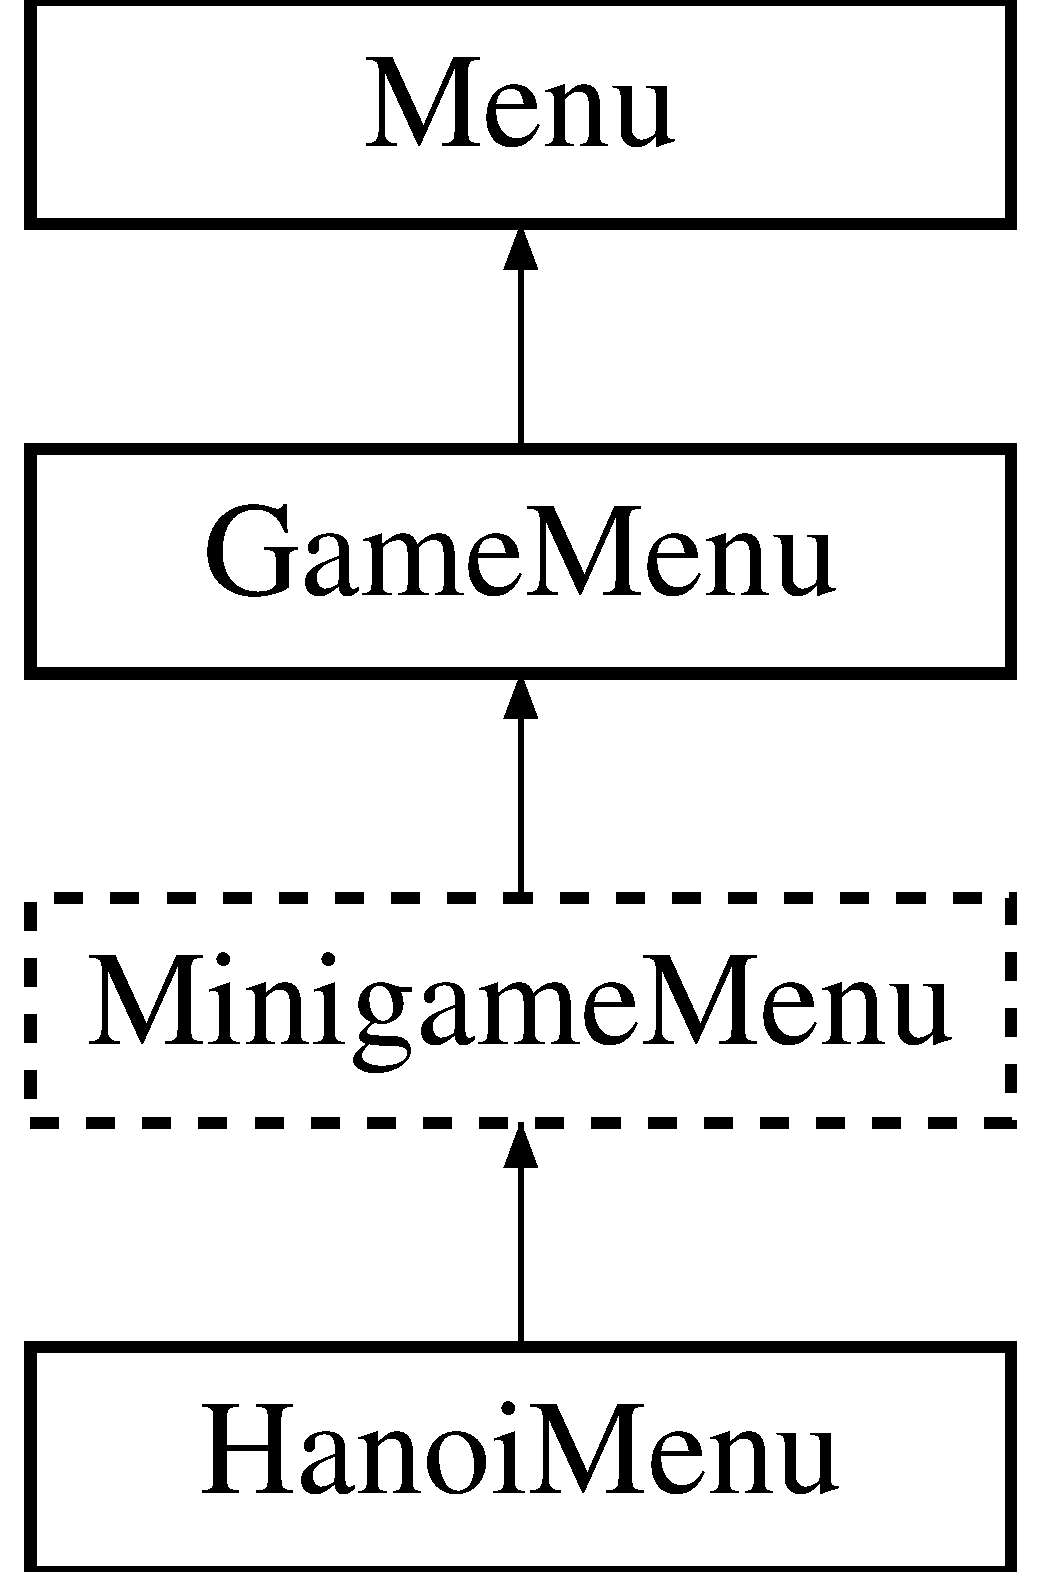
\includegraphics[height=4.000000cm]{classHanoiMenu}
\end{center}
\end{figure}
\subsection*{Public Member Functions}
\begin{DoxyCompactItemize}
\item 
\hypertarget{classHanoiMenu_a77aa5dc29b4c2954983e0471b8421d57}{\hyperlink{classHanoiMenu_a77aa5dc29b4c2954983e0471b8421d57}{Hanoi\-Menu} ()}\label{classHanoiMenu_a77aa5dc29b4c2954983e0471b8421d57}

\begin{DoxyCompactList}\small\item\em This is the default constructor. \end{DoxyCompactList}\item 
\hypertarget{classHanoiMenu_a80744afb9fe2111305ed0876ea371cd0}{virtual \hyperlink{classHanoiMenu_a80744afb9fe2111305ed0876ea371cd0}{$\sim$\-Hanoi\-Menu} ()}\label{classHanoiMenu_a80744afb9fe2111305ed0876ea371cd0}

\begin{DoxyCompactList}\small\item\em This is the virtual destructor. \end{DoxyCompactList}\item 
virtual void \hyperlink{classHanoiMenu_a1b6275a079452173e058c14f3b822271}{Set\-Options} (map$<$ string $>$ Options\-List, string type)
\item 
virtual void \hyperlink{classHanoiMenu_a8d287d810bc4cf49775503470830e48f}{Handle\-Input} (istream \&is)
\end{DoxyCompactItemize}
\subsection*{Additional Inherited Members}


\subsection{Detailed Description}
This is the menu class for the \hyperlink{classHanoi}{Hanoi} minigame. 

\subsection{Member Function Documentation}
\hypertarget{classHanoiMenu_a8d287d810bc4cf49775503470830e48f}{\index{Hanoi\-Menu@{Hanoi\-Menu}!Handle\-Input@{Handle\-Input}}
\index{Handle\-Input@{Handle\-Input}!HanoiMenu@{Hanoi\-Menu}}
\subsubsection[{Handle\-Input}]{\setlength{\rightskip}{0pt plus 5cm}virtual void Hanoi\-Menu\-::\-Handle\-Input (
\begin{DoxyParamCaption}
\item[{istream \&}]{is}
\end{DoxyParamCaption}
)\hspace{0.3cm}{\ttfamily [virtual]}}}\label{classHanoiMenu_a8d287d810bc4cf49775503470830e48f}
This function handles the input for the menu options. 
\begin{DoxyParams}[1]{Parameters}
\mbox{\tt in,out}  & {\em is} & The in-\/stream operator to read the input. \\
\hline
\end{DoxyParams}


Implements \hyperlink{classMinigameMenu_a3f854c4eefb0f3110cd085b3cfe56460}{Minigame\-Menu}.

\hypertarget{classHanoiMenu_a1b6275a079452173e058c14f3b822271}{\index{Hanoi\-Menu@{Hanoi\-Menu}!Set\-Options@{Set\-Options}}
\index{Set\-Options@{Set\-Options}!HanoiMenu@{Hanoi\-Menu}}
\subsubsection[{Set\-Options}]{\setlength{\rightskip}{0pt plus 5cm}virtual void Hanoi\-Menu\-::\-Set\-Options (
\begin{DoxyParamCaption}
\item[{map$<$ string $>$}]{Options\-List, }
\item[{string}]{type}
\end{DoxyParamCaption}
)\hspace{0.3cm}{\ttfamily [virtual]}}}\label{classHanoiMenu_a1b6275a079452173e058c14f3b822271}
This function sets the specific options for the \hyperlink{classMenu}{Menu} type. 
\begin{DoxyParams}[1]{Parameters}
\mbox{\tt in}  & {\em Options\-List} & A map of all the options for the current menu. Each option has a unique key to make input easier. \\
\hline
\mbox{\tt in}  & {\em type} & This denotes the type of menu to display. \\
\hline
\end{DoxyParams}


Implements \hyperlink{classMinigameMenu_a29820b5b338dec978b585f7a0df7b81e}{Minigame\-Menu}.



The documentation for this class was generated from the following file\-:\begin{DoxyCompactItemize}
\item 
Menu/Hanoi\-Menu.\-h\end{DoxyCompactItemize}

\hypertarget{classHanoiTest}{\section{Hanoi\-Test Class Reference}
\label{classHanoiTest}\index{Hanoi\-Test@{Hanoi\-Test}}
}


{\ttfamily \#include $<$Hanoi\-Test.\-h$>$}

Inheritance diagram for Hanoi\-Test\-:\begin{figure}[H]
\begin{center}
\leavevmode
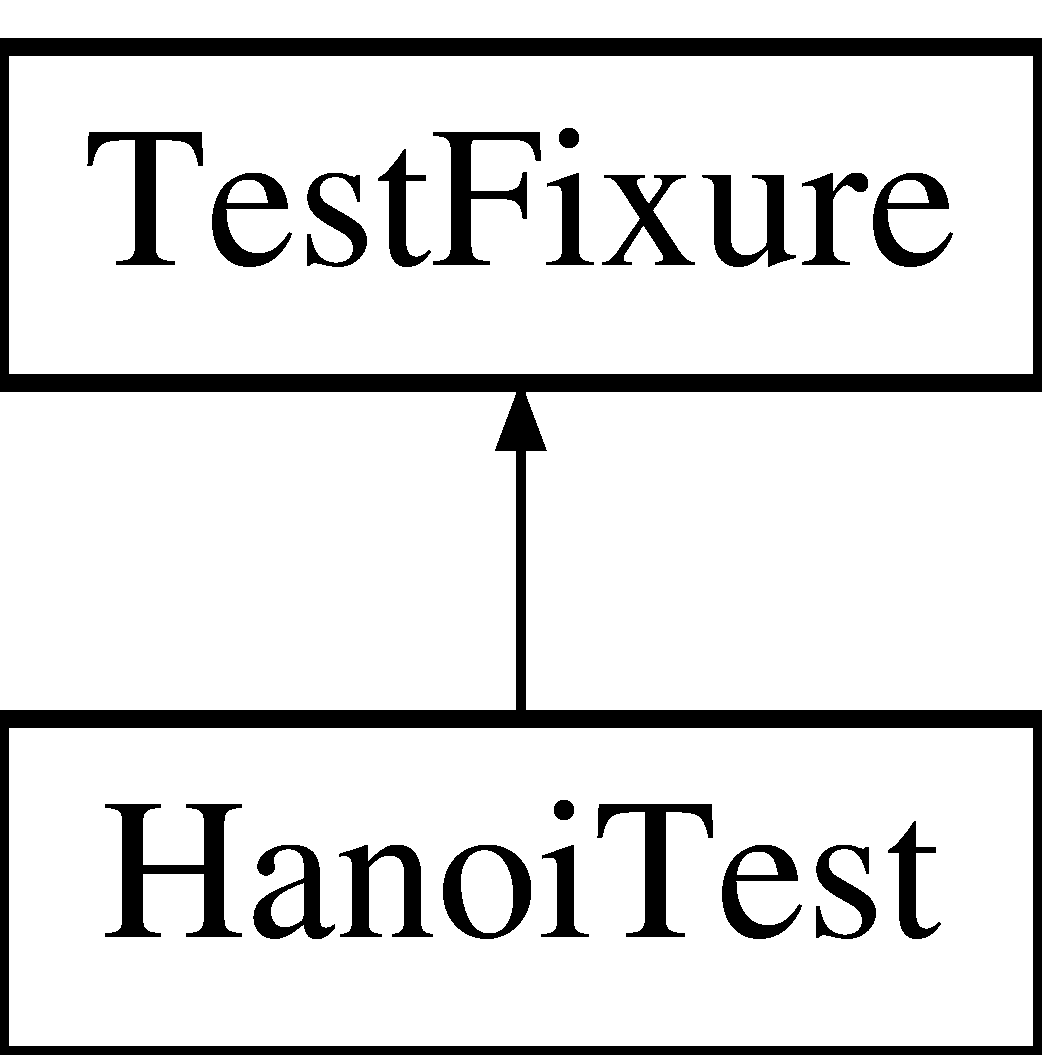
\includegraphics[height=2.000000cm]{classHanoiTest}
\end{center}
\end{figure}
\subsection*{Public Member Functions}
\begin{DoxyCompactItemize}
\item 
\hypertarget{classHanoiTest_a4b20d56cb0865c484c42f573699c9eda}{void {\bfseries Set\-Up} ()}\label{classHanoiTest_a4b20d56cb0865c484c42f573699c9eda}

\item 
\hypertarget{classHanoiTest_a7c51427b14c30753298e703edcb95f19}{void {\bfseries Test\-Run\-Game} ()}\label{classHanoiTest_a7c51427b14c30753298e703edcb95f19}

\end{DoxyCompactItemize}
\subsection*{Public Attributes}
\begin{DoxyCompactItemize}
\item 
\hypertarget{classHanoiTest_a4286e0f6ecc226a3d4848f2fb29f263b}{\hyperlink{classHanoi}{Hanoi} {\bfseries Game}}\label{classHanoiTest_a4286e0f6ecc226a3d4848f2fb29f263b}

\item 
\hypertarget{classHanoiTest_a0e37b5371b33e3ae17096aadf3d53bcf}{std\-::vector$<$ int $>$\-::size\-\_\-type {\bfseries indx}}\label{classHanoiTest_a0e37b5371b33e3ae17096aadf3d53bcf}

\end{DoxyCompactItemize}


\subsection{Detailed Description}
\begin{DoxyAuthor}{Author}
Tyler Siwy 
\end{DoxyAuthor}
\begin{DoxyDate}{Date}
Nov 9, 2017 
\end{DoxyDate}


The documentation for this class was generated from the following file\-:\begin{DoxyCompactItemize}
\item 
Puzzles/Hanoi\-Test.\-h\end{DoxyCompactItemize}

\hypertarget{classHealthPotion}{\section{Health\-Potion Class Reference}
\label{classHealthPotion}\index{Health\-Potion@{Health\-Potion}}
}


Subclass of \hyperlink{classConsumable}{Consumable} to represent an in game health potion.  




{\ttfamily \#include $<$My\-Consumables.\-h$>$}

Inheritance diagram for Health\-Potion\-:\begin{figure}[H]
\begin{center}
\leavevmode
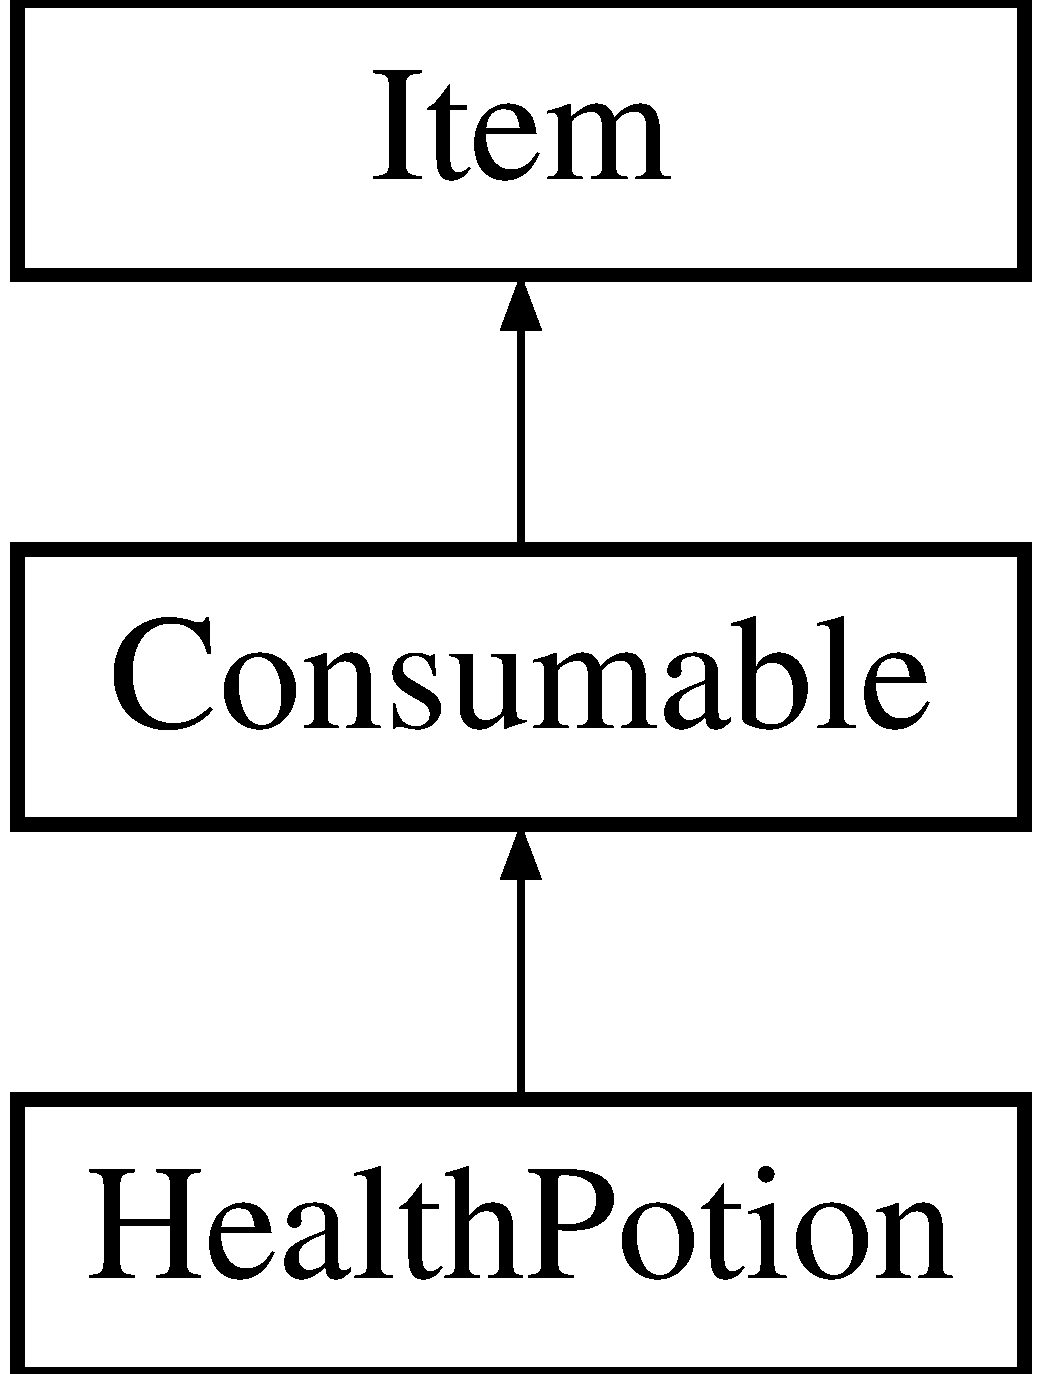
\includegraphics[height=3.000000cm]{classHealthPotion}
\end{center}
\end{figure}
\subsection*{Public Member Functions}
\begin{DoxyCompactItemize}
\item 
\hyperlink{classHealthPotion_a99e942956f7f1e07dd13c46daae08713}{Health\-Potion} ()
\begin{DoxyCompactList}\small\item\em \hyperlink{classHealthPotion}{Health\-Potion} Constructor. \end{DoxyCompactList}\item 
bool \hyperlink{classHealthPotion_a6fee598a4d80425364c72da18b883615}{Use} (\hyperlink{classCharacter}{Character} $\ast$target)
\end{DoxyCompactItemize}
\subsection*{Additional Inherited Members}


\subsection{Detailed Description}
Subclass of \hyperlink{classConsumable}{Consumable} to represent an in game health potion. 

\subsection{Constructor \& Destructor Documentation}
\hypertarget{classHealthPotion_a99e942956f7f1e07dd13c46daae08713}{\index{Health\-Potion@{Health\-Potion}!Health\-Potion@{Health\-Potion}}
\index{Health\-Potion@{Health\-Potion}!HealthPotion@{Health\-Potion}}
\subsubsection[{Health\-Potion}]{\setlength{\rightskip}{0pt plus 5cm}Health\-Potion\-::\-Health\-Potion (
\begin{DoxyParamCaption}
{}
\end{DoxyParamCaption}
)}}\label{classHealthPotion_a99e942956f7f1e07dd13c46daae08713}


\hyperlink{classHealthPotion}{Health\-Potion} Constructor. 



\subsection{Member Function Documentation}
\hypertarget{classHealthPotion_a6fee598a4d80425364c72da18b883615}{\index{Health\-Potion@{Health\-Potion}!Use@{Use}}
\index{Use@{Use}!HealthPotion@{Health\-Potion}}
\subsubsection[{Use}]{\setlength{\rightskip}{0pt plus 5cm}bool Health\-Potion\-::\-Use (
\begin{DoxyParamCaption}
\item[{{\bf Character} $\ast$}]{target}
\end{DoxyParamCaption}
)\hspace{0.3cm}{\ttfamily [virtual]}}}\label{classHealthPotion_a6fee598a4d80425364c72da18b883615}
Defines what happens when the health potion is used 
\begin{DoxyParams}[1]{Parameters}
\mbox{\tt in}  & {\em target} & The \hyperlink{classCharacter}{Character} that the health potion is used on \\
\hline
\end{DoxyParams}
\begin{DoxyReturn}{Returns}
true if use was successfull 
\end{DoxyReturn}


Implements \hyperlink{classItem_abd3f52dd7fa25d497f2070e95d44ac03}{Item}.



The documentation for this class was generated from the following files\-:\begin{DoxyCompactItemize}
\item 
/home/rigt2720/\-Kodika/\-Item/\hyperlink{MyConsumables_8h}{My\-Consumables.\-h}\item 
/home/rigt2720/\-Kodika/\-Item/\hyperlink{MyConsumables_8cpp}{My\-Consumables.\-cpp}\end{DoxyCompactItemize}

\hypertarget{classImage}{\section{Image Class Reference}
\label{classImage}\index{Image@{Image}}
}


The \hyperlink{classImage}{Image} class represents a 2\-D vector that displays an image on screen.  




{\ttfamily \#include $<$Image.\-h$>$}

Inheritance diagram for Image\-:\begin{figure}[H]
\begin{center}
\leavevmode
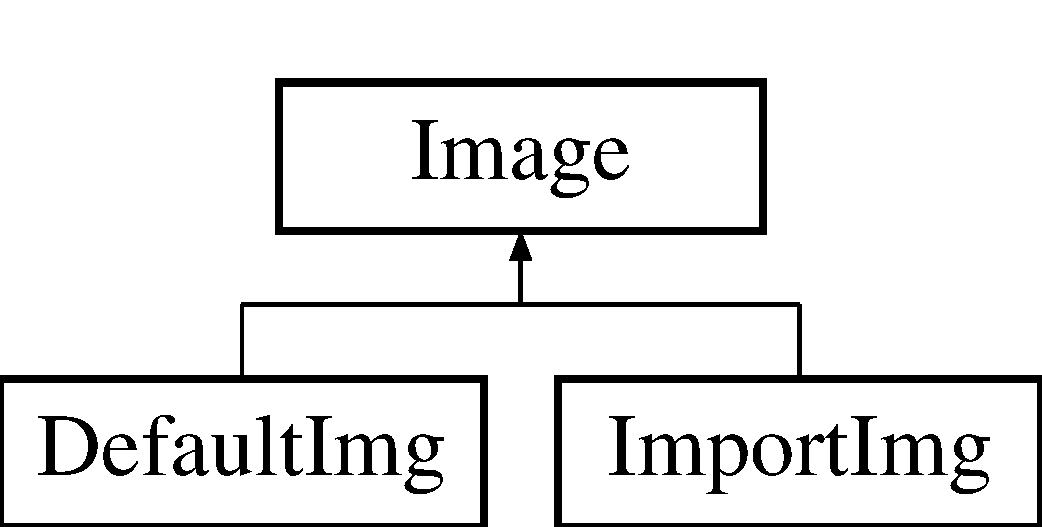
\includegraphics[height=2.000000cm]{classImage}
\end{center}
\end{figure}
\subsection*{Public Member Functions}
\begin{DoxyCompactItemize}
\item 
\hyperlink{classImage_a13aa6167bbc77b7a311a181d67caa058}{Image} (int h=3, int w=6, char c= '$\ast$')
\item 
\hyperlink{classImage_ad9a2ebd07a4f458ba24d91af0122418e}{Image} (\hyperlink{classImage}{Image} \&img)
\item 
\hyperlink{classImage_aa44ed77d00d96d2c878b050835f828c4}{Image} (const \hyperlink{classImage}{Image} \&img)
\item 
virtual \hyperlink{classImage_a0294f63700543e11c0f0da85601c7ae5}{$\sim$\-Image} ()
\begin{DoxyCompactList}\small\item\em Virtual Destructor. \end{DoxyCompactList}\item 
virtual \hyperlink{classImage}{Image} \& \hyperlink{classImage_a645773587ffefda3891bfc7f6cc541bb}{operator=} (const \hyperlink{classImage}{Image} \&img)
\item 
virtual void \hyperlink{classImage_a057cb6b10590608656ff2a7aa159f515}{Draw} (\hyperlink{classScreen}{Screen} \&scr)
\item 
virtual void \hyperlink{classImage_a1e3d4ae638b3fc1fbee81c509c1551f6}{Draw} (\hyperlink{classScreen}{Screen} \&scr, int y, int x)
\item 
virtual void \hyperlink{classImage_ad20f87dc888d01cadc829f18d23066dc}{Draw} (\hyperlink{classImage}{Image} \&img)
\item 
virtual void \hyperlink{classImage_a2e863a5b8287ca3adb08fdaae513f437}{Draw} (\hyperlink{classImage}{Image} \&img, int y, int x)
\item 
virtual void \hyperlink{classImage_a6bb7dff9e4c4c31b2d63d7b0a330ef89}{Create} ()
\begin{DoxyCompactList}\small\item\em Function to create the image. \end{DoxyCompactList}\item 
void \hyperlink{classImage_a16f8719e59b1180aa7e0e2fdf3e4d421}{Draw\-Border} (char \hyperlink{classImage_a2d2bff881014df332b1086483d0eb0e9}{ch})
\item 
void \hyperlink{classImage_a118986dafc30b76c4aa5e7453236a8b2}{Erase} ()
\begin{DoxyCompactList}\small\item\em Function to erase the contents of the image and replace with spaces. \end{DoxyCompactList}\item 
void \hyperlink{classImage_a39486b75d05a1d3c0206a9ce909f3571}{Fill} (char \hyperlink{classImage_a2d2bff881014df332b1086483d0eb0e9}{ch})
\item 
void \hyperlink{classImage_a4fbbffe74cd76d884f1e2a96d0bb6c09}{Set} (int y, int x, char \hyperlink{classImage_a2d2bff881014df332b1086483d0eb0e9}{ch})
\begin{DoxyCompactList}\small\item\em Sets the characters at the given location to the given character. \end{DoxyCompactList}\item 
void \hyperlink{classImage_ab68774143becf8906bf8b1931511cb66}{Set\-Origin} (\hyperlink{classScreen}{Screen} \&scr, int y, int x)
\item 
void \hyperlink{classImage_adfe7a1b2cf0bd7893cdd55a646da8d77}{Set\-Origin} (\hyperlink{classImage}{Image} \&img, int y, int x)
\item 
void \hyperlink{classImage_a1c7560c1e8f95eb0a879fb4fac72fa28}{Flip\-Horiz} ()
\begin{DoxyCompactList}\small\item\em Function that flips an image horizontally. \end{DoxyCompactList}\item 
void \hyperlink{classImage_a94fe8fd85b9ef3461c2576d29ebd3a86}{Flip\-Vert} ()
\begin{DoxyCompactList}\small\item\em Function that flips an image vertically. \end{DoxyCompactList}\item 
void \hyperlink{classImage_a605b3921fed112ffb8a371341c68eb4c}{Align\-Left} (\hyperlink{classScreen}{Screen} \&scr)
\item 
void \hyperlink{classImage_abbb7cdfe276a373ad9b50d5be641eeef}{Align\-Right} (\hyperlink{classScreen}{Screen} \&scr)
\item 
void \hyperlink{classImage_a691da8aebb2d92b7471da96a19e0fc22}{Align\-Center} (\hyperlink{classScreen}{Screen} \&scr)
\item 
void \hyperlink{classImage_a5048f1f5a975185d24a08247dbce1568}{Align\-Top} (\hyperlink{classScreen}{Screen} \&scr)
\item 
void \hyperlink{classImage_adfd7cfe672b8950fa7cfcff8022169b0}{Align\-Bottom} (\hyperlink{classScreen}{Screen} \&scr)
\item 
void \hyperlink{classImage_a863eee8dfbe927d73fba705844eb3117}{Align\-Left} (\hyperlink{classImage}{Image} \&img)
\item 
void \hyperlink{classImage_a171b44f5d1ac53bfa9984a87c9786dd1}{Align\-Right} (\hyperlink{classImage}{Image} \&img)
\item 
void \hyperlink{classImage_a7471581b8a028a79fd87d741ae825e23}{Align\-Center} (\hyperlink{classImage}{Image} \&img)
\item 
void \hyperlink{classImage_a4607fa422c54fb4bf0412edd47214b40}{Align\-Center} (\hyperlink{classImage}{Image} \&img, int x, int y)
\item 
void \hyperlink{classImage_a12f3de115677e508268f5b7d3485b483}{Align\-Top} (\hyperlink{classImage}{Image} \&img)
\item 
void \hyperlink{classImage_a1bb0179923b51be9159fbd74b6f4f91f}{Align\-Bottom} (\hyperlink{classImage}{Image} \&img)
\item 
void \hyperlink{classImage_aed099dcc3c5113b7171daa35460df948}{Shift\-Down} (\hyperlink{classScreen}{Screen} \&scr, int num)
\item 
void \hyperlink{classImage_a1dc60415fb8f71c1c9345382be4ee32f}{Shift\-Right} (\hyperlink{classScreen}{Screen} \&scr, int num)
\item 
void \hyperlink{classImage_ad3fec1f163c82a6dc376e1727e42de30}{Shift\-Down} (\hyperlink{classImage}{Image} \&img, int num)
\item 
void \hyperlink{classImage_ae905765bb51e09a8252dcb157b2bcf28}{Shift\-Right} (\hyperlink{classImage}{Image} \&img, int num)
\item 
void \hyperlink{classImage_a8b15a9bbf2a56bd2105bbc1114bba173}{Shift\-Up} (int num)
\item 
void \hyperlink{classImage_a1bc3f79eeff5bfcc430299cb149071f5}{Shift\-Left} (int num)
\item 
int \hyperlink{classImage_a91b5bb5c3fef2795ec9838763536ed78}{Get\-Rows} () const 
\begin{DoxyCompactList}\small\item\em Returns the height of the image. \end{DoxyCompactList}\item 
int \hyperlink{classImage_a5377ce45ff29db084776e675b413f165}{Get\-Cols} () const 
\begin{DoxyCompactList}\small\item\em Returns the width of the image. \end{DoxyCompactList}\item 
void \hyperlink{classImage_a5c723d560bde4b6aa45f3eaa36ffb4f2}{Fix\-Slants} ()
\begin{DoxyCompactList}\small\item\em Helper function to switch the slant characters. \end{DoxyCompactList}\end{DoxyCompactItemize}
\subsection*{Public Attributes}
\begin{DoxyCompactItemize}
\item 
vector$<$ vector$<$ char $>$ $>$ \hyperlink{classImage_ac3bad7d8544990b7be9e9c5ee0fb26b8}{Img}
\begin{DoxyCompactList}\small\item\em The image -\/ publically availiable to allow access to locations. \end{DoxyCompactList}\item 
int \hyperlink{classImage_a0488098c125477f82fc6ca8e14cc170f}{screen\-X} = 0
\begin{DoxyCompactList}\small\item\em The screen x coordinate to draw on. \end{DoxyCompactList}\item 
int \hyperlink{classImage_a4c5bb89eba006c3768c2f36ef54d2c5b}{screen\-Y} = 0
\begin{DoxyCompactList}\small\item\em The screen y coordinate to draw on. \end{DoxyCompactList}\end{DoxyCompactItemize}
\subsection*{Protected Member Functions}
\begin{DoxyCompactItemize}
\item 
bool \hyperlink{classImage_aa723637c3d64e1290dbfc67238321413}{Is\-Even} (const int \&num) const 
\end{DoxyCompactItemize}
\subsection*{Protected Attributes}
\begin{DoxyCompactItemize}
\item 
int \hyperlink{classImage_a51df43db420c9c0b57536cb2dd36de5c}{height}
\begin{DoxyCompactList}\small\item\em The height of the image. \end{DoxyCompactList}\item 
int \hyperlink{classImage_ab8d12f635013c04159cd4d3d972bac88}{width}
\begin{DoxyCompactList}\small\item\em The width of the image. \end{DoxyCompactList}\item 
char \hyperlink{classImage_a2d2bff881014df332b1086483d0eb0e9}{ch}
\begin{DoxyCompactList}\small\item\em The character used to draw the image. \end{DoxyCompactList}\end{DoxyCompactItemize}


\subsection{Detailed Description}
The \hyperlink{classImage}{Image} class represents a 2\-D vector that displays an image on screen. 

\subsection{Constructor \& Destructor Documentation}
\hypertarget{classImage_a13aa6167bbc77b7a311a181d67caa058}{\index{Image@{Image}!Image@{Image}}
\index{Image@{Image}!Image@{Image}}
\subsubsection[{Image}]{\setlength{\rightskip}{0pt plus 5cm}Image\-::\-Image (
\begin{DoxyParamCaption}
\item[{int}]{h = {\ttfamily 3}, }
\item[{int}]{w = {\ttfamily 6}, }
\item[{char}]{c = {\ttfamily '$\ast$'}}
\end{DoxyParamCaption}
)}}\label{classImage_a13aa6167bbc77b7a311a181d67caa058}
Constructs an \hyperlink{classImage}{Image} object from the given dimensions 
\begin{DoxyParams}[1]{Parameters}
\mbox{\tt in}  & {\em h} & the height of the image, default to 3 \\
\hline
\mbox{\tt in}  & {\em w} & the width of the image, default to 6\\
\hline
\end{DoxyParams}
Default Constructor 
\begin{DoxyParams}[1]{Parameters}
\mbox{\tt in}  & {\em h} & the height of the image \\
\hline
\mbox{\tt in}  & {\em w} & the width of the image \\
\hline
\mbox{\tt in}  & {\em c} & the character to be drawn with \\
\hline
\end{DoxyParams}
\hypertarget{classImage_ad9a2ebd07a4f458ba24d91af0122418e}{\index{Image@{Image}!Image@{Image}}
\index{Image@{Image}!Image@{Image}}
\subsubsection[{Image}]{\setlength{\rightskip}{0pt plus 5cm}Image\-::\-Image (
\begin{DoxyParamCaption}
\item[{{\bf Image} \&}]{image}
\end{DoxyParamCaption}
)}}\label{classImage_ad9a2ebd07a4f458ba24d91af0122418e}
Copy constructor duplicates a given picture 
\begin{DoxyParams}[1]{Parameters}
\mbox{\tt in}  & {\em img} & the image to copy from\\
\hline
\end{DoxyParams}
Copy Constructor for the image 
\begin{DoxyParams}[1]{Parameters}
\mbox{\tt in}  & {\em image} & the image to be copied from \\
\hline
\end{DoxyParams}
\hypertarget{classImage_aa44ed77d00d96d2c878b050835f828c4}{\index{Image@{Image}!Image@{Image}}
\index{Image@{Image}!Image@{Image}}
\subsubsection[{Image}]{\setlength{\rightskip}{0pt plus 5cm}Image\-::\-Image (
\begin{DoxyParamCaption}
\item[{const {\bf Image} \&}]{image}
\end{DoxyParamCaption}
)}}\label{classImage_aa44ed77d00d96d2c878b050835f828c4}
Copy constructor duplicates a given picture 
\begin{DoxyParams}[1]{Parameters}
\mbox{\tt in}  & {\em img} & the image to copy from\\
\hline
\end{DoxyParams}
Copy Constructor for the image 
\begin{DoxyParams}[1]{Parameters}
\mbox{\tt in}  & {\em image} & the image to be copied from \\
\hline
\end{DoxyParams}
\hypertarget{classImage_a0294f63700543e11c0f0da85601c7ae5}{\index{Image@{Image}!$\sim$\-Image@{$\sim$\-Image}}
\index{$\sim$\-Image@{$\sim$\-Image}!Image@{Image}}
\subsubsection[{$\sim$\-Image}]{\setlength{\rightskip}{0pt plus 5cm}Image\-::$\sim$\-Image (
\begin{DoxyParamCaption}
{}
\end{DoxyParamCaption}
)\hspace{0.3cm}{\ttfamily [virtual]}}}\label{classImage_a0294f63700543e11c0f0da85601c7ae5}


Virtual Destructor. 

Destructor. 

\subsection{Member Function Documentation}
\hypertarget{classImage_adfd7cfe672b8950fa7cfcff8022169b0}{\index{Image@{Image}!Align\-Bottom@{Align\-Bottom}}
\index{Align\-Bottom@{Align\-Bottom}!Image@{Image}}
\subsubsection[{Align\-Bottom}]{\setlength{\rightskip}{0pt plus 5cm}void Image\-::\-Align\-Bottom (
\begin{DoxyParamCaption}
\item[{{\bf Screen} \&}]{screen}
\end{DoxyParamCaption}
)}}\label{classImage_adfd7cfe672b8950fa7cfcff8022169b0}
Helper function to align the image to the bottom 
\begin{DoxyParams}[1]{Parameters}
\mbox{\tt in}  & {\em scr} & the screen to draw to\\
\hline
\end{DoxyParams}
Align the image to the bottom of the screen 
\begin{DoxyParams}[1]{Parameters}
\mbox{\tt in}  & {\em screen} & used to align with \\
\hline
\end{DoxyParams}
\hypertarget{classImage_a1bb0179923b51be9159fbd74b6f4f91f}{\index{Image@{Image}!Align\-Bottom@{Align\-Bottom}}
\index{Align\-Bottom@{Align\-Bottom}!Image@{Image}}
\subsubsection[{Align\-Bottom}]{\setlength{\rightskip}{0pt plus 5cm}void Image\-::\-Align\-Bottom (
\begin{DoxyParamCaption}
\item[{{\bf Image} \&}]{img}
\end{DoxyParamCaption}
)}}\label{classImage_a1bb0179923b51be9159fbd74b6f4f91f}
Helper function to align the image to the bottom 
\begin{DoxyParams}[1]{Parameters}
\mbox{\tt in}  & {\em img} & the image to draw to\\
\hline
\end{DoxyParams}
Align the image to the bottom of the image 
\begin{DoxyParams}[1]{Parameters}
\mbox{\tt in}  & {\em img} & used to align with \\
\hline
\end{DoxyParams}
\hypertarget{classImage_a691da8aebb2d92b7471da96a19e0fc22}{\index{Image@{Image}!Align\-Center@{Align\-Center}}
\index{Align\-Center@{Align\-Center}!Image@{Image}}
\subsubsection[{Align\-Center}]{\setlength{\rightskip}{0pt plus 5cm}void Image\-::\-Align\-Center (
\begin{DoxyParamCaption}
\item[{{\bf Screen} \&}]{screen}
\end{DoxyParamCaption}
)}}\label{classImage_a691da8aebb2d92b7471da96a19e0fc22}
Helper function to align the image center 
\begin{DoxyParams}[1]{Parameters}
\mbox{\tt in}  & {\em scr} & the screen to align to\\
\hline
\end{DoxyParams}
Align the image to the center of the screen 
\begin{DoxyParams}[1]{Parameters}
\mbox{\tt in}  & {\em screen} & checks to ensure the bounds aren't exceeded \\
\hline
\end{DoxyParams}
\hypertarget{classImage_a7471581b8a028a79fd87d741ae825e23}{\index{Image@{Image}!Align\-Center@{Align\-Center}}
\index{Align\-Center@{Align\-Center}!Image@{Image}}
\subsubsection[{Align\-Center}]{\setlength{\rightskip}{0pt plus 5cm}void Image\-::\-Align\-Center (
\begin{DoxyParamCaption}
\item[{{\bf Image} \&}]{img}
\end{DoxyParamCaption}
)}}\label{classImage_a7471581b8a028a79fd87d741ae825e23}
Helper function to align the image to the center 
\begin{DoxyParams}[1]{Parameters}
\mbox{\tt in}  & {\em img} & the image to align to\\
\hline
\end{DoxyParams}
Align the image to the center of the given image 
\begin{DoxyParams}[1]{Parameters}
\mbox{\tt in}  & {\em image} & checks to ensure the bounds aren't exceeded \\
\hline
\end{DoxyParams}
\hypertarget{classImage_a4607fa422c54fb4bf0412edd47214b40}{\index{Image@{Image}!Align\-Center@{Align\-Center}}
\index{Align\-Center@{Align\-Center}!Image@{Image}}
\subsubsection[{Align\-Center}]{\setlength{\rightskip}{0pt plus 5cm}void Image\-::\-Align\-Center (
\begin{DoxyParamCaption}
\item[{{\bf Image} \&}]{img, }
\item[{int}]{x, }
\item[{int}]{y}
\end{DoxyParamCaption}
)}}\label{classImage_a4607fa422c54fb4bf0412edd47214b40}
Helper function to align the image center 
\begin{DoxyParams}[1]{Parameters}
\mbox{\tt in}  & {\em img} & the image to align to\\
\hline
\end{DoxyParams}
Align the image to the center of the given image 
\begin{DoxyParams}[1]{Parameters}
\mbox{\tt in}  & {\em image} & checks to ensure the bounds aren't exceeded \\
\hline
\mbox{\tt in}  & {\em x} & the x coordinate to center around \\
\hline
\mbox{\tt in}  & {\em y} & the y coordinate to center around \\
\hline
\end{DoxyParams}
\hypertarget{classImage_a605b3921fed112ffb8a371341c68eb4c}{\index{Image@{Image}!Align\-Left@{Align\-Left}}
\index{Align\-Left@{Align\-Left}!Image@{Image}}
\subsubsection[{Align\-Left}]{\setlength{\rightskip}{0pt plus 5cm}void Image\-::\-Align\-Left (
\begin{DoxyParamCaption}
\item[{{\bf Screen} \&}]{screen}
\end{DoxyParamCaption}
)}}\label{classImage_a605b3921fed112ffb8a371341c68eb4c}
Helper function to align the image left 
\begin{DoxyParams}[1]{Parameters}
\mbox{\tt in}  & {\em scr} & the screen to align to\\
\hline
\end{DoxyParams}
Align the image to the left of the screen 
\begin{DoxyParams}[1]{Parameters}
\mbox{\tt in}  & {\em screen} & used to align with \\
\hline
\end{DoxyParams}
\hypertarget{classImage_a863eee8dfbe927d73fba705844eb3117}{\index{Image@{Image}!Align\-Left@{Align\-Left}}
\index{Align\-Left@{Align\-Left}!Image@{Image}}
\subsubsection[{Align\-Left}]{\setlength{\rightskip}{0pt plus 5cm}void Image\-::\-Align\-Left (
\begin{DoxyParamCaption}
\item[{{\bf Image} \&}]{img}
\end{DoxyParamCaption}
)}}\label{classImage_a863eee8dfbe927d73fba705844eb3117}
Helper function to align the image left 
\begin{DoxyParams}[1]{Parameters}
\mbox{\tt in}  & {\em img} & the screen to align to\\
\hline
\end{DoxyParams}
Align the image to the left of the given image 
\begin{DoxyParams}[1]{Parameters}
\mbox{\tt in}  & {\em image} & checks to ensure the bounds aren't exceeded \\
\hline
\end{DoxyParams}
\hypertarget{classImage_abbb7cdfe276a373ad9b50d5be641eeef}{\index{Image@{Image}!Align\-Right@{Align\-Right}}
\index{Align\-Right@{Align\-Right}!Image@{Image}}
\subsubsection[{Align\-Right}]{\setlength{\rightskip}{0pt plus 5cm}void Image\-::\-Align\-Right (
\begin{DoxyParamCaption}
\item[{{\bf Screen} \&}]{screen}
\end{DoxyParamCaption}
)}}\label{classImage_abbb7cdfe276a373ad9b50d5be641eeef}
Helper function to align the image right 
\begin{DoxyParams}[1]{Parameters}
\mbox{\tt in}  & {\em scr} & the screen to align to\\
\hline
\end{DoxyParams}
Align the image to the right of the screen 
\begin{DoxyParams}[1]{Parameters}
\mbox{\tt in}  & {\em screen} & used to align with \\
\hline
\end{DoxyParams}
\hypertarget{classImage_a171b44f5d1ac53bfa9984a87c9786dd1}{\index{Image@{Image}!Align\-Right@{Align\-Right}}
\index{Align\-Right@{Align\-Right}!Image@{Image}}
\subsubsection[{Align\-Right}]{\setlength{\rightskip}{0pt plus 5cm}void Image\-::\-Align\-Right (
\begin{DoxyParamCaption}
\item[{{\bf Image} \&}]{img}
\end{DoxyParamCaption}
)}}\label{classImage_a171b44f5d1ac53bfa9984a87c9786dd1}
Helper function to align the image right 
\begin{DoxyParams}[1]{Parameters}
\mbox{\tt in}  & {\em img} & the image to align to\\
\hline
\end{DoxyParams}
Align the image to the right of the given image 
\begin{DoxyParams}[1]{Parameters}
\mbox{\tt in}  & {\em image} & checks to ensure the bounds aren't exceeded \\
\hline
\end{DoxyParams}
\hypertarget{classImage_a5048f1f5a975185d24a08247dbce1568}{\index{Image@{Image}!Align\-Top@{Align\-Top}}
\index{Align\-Top@{Align\-Top}!Image@{Image}}
\subsubsection[{Align\-Top}]{\setlength{\rightskip}{0pt plus 5cm}void Image\-::\-Align\-Top (
\begin{DoxyParamCaption}
\item[{{\bf Screen} \&}]{screen}
\end{DoxyParamCaption}
)}}\label{classImage_a5048f1f5a975185d24a08247dbce1568}
Helper function to align the image to the top 
\begin{DoxyParams}[1]{Parameters}
\mbox{\tt in}  & {\em scr} & the screen to draw to\\
\hline
\end{DoxyParams}
Align the image to the top of the screen 
\begin{DoxyParams}[1]{Parameters}
\mbox{\tt in}  & {\em screen} & used to align with \\
\hline
\end{DoxyParams}
\hypertarget{classImage_a12f3de115677e508268f5b7d3485b483}{\index{Image@{Image}!Align\-Top@{Align\-Top}}
\index{Align\-Top@{Align\-Top}!Image@{Image}}
\subsubsection[{Align\-Top}]{\setlength{\rightskip}{0pt plus 5cm}void Image\-::\-Align\-Top (
\begin{DoxyParamCaption}
\item[{{\bf Image} \&}]{img}
\end{DoxyParamCaption}
)}}\label{classImage_a12f3de115677e508268f5b7d3485b483}
Helper function to align the image to the top 
\begin{DoxyParams}[1]{Parameters}
\mbox{\tt in}  & {\em img} & the image to align to\\
\hline
\end{DoxyParams}
Align the image to the top of the image 
\begin{DoxyParams}[1]{Parameters}
\mbox{\tt in}  & {\em img} & used to align with \\
\hline
\end{DoxyParams}
\hypertarget{classImage_a6bb7dff9e4c4c31b2d63d7b0a330ef89}{\index{Image@{Image}!Create@{Create}}
\index{Create@{Create}!Image@{Image}}
\subsubsection[{Create}]{\setlength{\rightskip}{0pt plus 5cm}void Image\-::\-Create (
\begin{DoxyParamCaption}
{}
\end{DoxyParamCaption}
)\hspace{0.3cm}{\ttfamily [virtual]}}}\label{classImage_a6bb7dff9e4c4c31b2d63d7b0a330ef89}


Function to create the image. 

Function that fills in the vector that makes up the image. 

Reimplemented in \hyperlink{classDefaultImg_a9ab21b397e0d23831b2944b651058b89}{Default\-Img}, and \hyperlink{classImportImg_a7e1cc1bf176cedb14938519950719fa2}{Import\-Img}.

\hypertarget{classImage_a057cb6b10590608656ff2a7aa159f515}{\index{Image@{Image}!Draw@{Draw}}
\index{Draw@{Draw}!Image@{Image}}
\subsubsection[{Draw}]{\setlength{\rightskip}{0pt plus 5cm}void Image\-::\-Draw (
\begin{DoxyParamCaption}
\item[{{\bf Screen} \&}]{screen}
\end{DoxyParamCaption}
)\hspace{0.3cm}{\ttfamily [virtual]}}}\label{classImage_a057cb6b10590608656ff2a7aa159f515}
Helper function to draw onto the \hyperlink{classScreen}{Screen} object 
\begin{DoxyParams}[1]{Parameters}
\mbox{\tt in}  & {\em scr} & the screen to draw on\\
\hline
\end{DoxyParams}
Function to draw the image to the screen 
\begin{DoxyParams}[1]{Parameters}
\mbox{\tt in}  & {\em screen} & the screen drawn on \\
\hline
\end{DoxyParams}
\hypertarget{classImage_a1e3d4ae638b3fc1fbee81c509c1551f6}{\index{Image@{Image}!Draw@{Draw}}
\index{Draw@{Draw}!Image@{Image}}
\subsubsection[{Draw}]{\setlength{\rightskip}{0pt plus 5cm}void Image\-::\-Draw (
\begin{DoxyParamCaption}
\item[{{\bf Screen} \&}]{screen, }
\item[{int}]{y, }
\item[{int}]{x}
\end{DoxyParamCaption}
)\hspace{0.3cm}{\ttfamily [virtual]}}}\label{classImage_a1e3d4ae638b3fc1fbee81c509c1551f6}
Helper function to draw onto the \hyperlink{classScreen}{Screen} object 
\begin{DoxyParams}[1]{Parameters}
\mbox{\tt in}  & {\em scr} & the screen to draw on \\
\hline
\mbox{\tt in}  & {\em x} & the x coordinate \\
\hline
\mbox{\tt in}  & {\em y} & the y coordinate\\
\hline
\end{DoxyParams}
Function to draw the image to the screen 
\begin{DoxyParams}[1]{Parameters}
\mbox{\tt in}  & {\em screen} & the screen drawn on \\
\hline
\mbox{\tt in}  & {\em y} & the y coordinate to begin drawing from \\
\hline
\mbox{\tt in}  & {\em x} & the x coordinate to begin drawing from \\
\hline
\end{DoxyParams}
\hypertarget{classImage_ad20f87dc888d01cadc829f18d23066dc}{\index{Image@{Image}!Draw@{Draw}}
\index{Draw@{Draw}!Image@{Image}}
\subsubsection[{Draw}]{\setlength{\rightskip}{0pt plus 5cm}void Image\-::\-Draw (
\begin{DoxyParamCaption}
\item[{{\bf Image} \&}]{img}
\end{DoxyParamCaption}
)\hspace{0.3cm}{\ttfamily [virtual]}}}\label{classImage_ad20f87dc888d01cadc829f18d23066dc}
Helper function to draw onto the \hyperlink{classScreen}{Screen} object 
\begin{DoxyParams}[1]{Parameters}
\mbox{\tt in}  & {\em img} & the screen to draw on\\
\hline
\end{DoxyParams}
Function to draw the image to the screen 
\begin{DoxyParams}[1]{Parameters}
\mbox{\tt in}  & {\em image} & the image drawn on \\
\hline
\end{DoxyParams}
\hypertarget{classImage_a2e863a5b8287ca3adb08fdaae513f437}{\index{Image@{Image}!Draw@{Draw}}
\index{Draw@{Draw}!Image@{Image}}
\subsubsection[{Draw}]{\setlength{\rightskip}{0pt plus 5cm}void Image\-::\-Draw (
\begin{DoxyParamCaption}
\item[{{\bf Image} \&}]{img, }
\item[{int}]{y, }
\item[{int}]{x}
\end{DoxyParamCaption}
)\hspace{0.3cm}{\ttfamily [virtual]}}}\label{classImage_a2e863a5b8287ca3adb08fdaae513f437}
Helper function to draw onto the \hyperlink{classScreen}{Screen} object 
\begin{DoxyParams}[1]{Parameters}
\mbox{\tt in}  & {\em img} & the screen to draw on \\
\hline
\mbox{\tt in}  & {\em x} & the x coordinate \\
\hline
\mbox{\tt in}  & {\em y} & the y coordinate\\
\hline
\end{DoxyParams}
Function to draw the image to the screen 
\begin{DoxyParams}[1]{Parameters}
\mbox{\tt in}  & {\em img} & the image drawn on \\
\hline
\mbox{\tt in}  & {\em y} & the y coordinate to begin drawing from \\
\hline
\mbox{\tt in}  & {\em x} & the x coordinate to begin drawing from \\
\hline
\end{DoxyParams}
\hypertarget{classImage_a16f8719e59b1180aa7e0e2fdf3e4d421}{\index{Image@{Image}!Draw\-Border@{Draw\-Border}}
\index{Draw\-Border@{Draw\-Border}!Image@{Image}}
\subsubsection[{Draw\-Border}]{\setlength{\rightskip}{0pt plus 5cm}void Image\-::\-Draw\-Border (
\begin{DoxyParamCaption}
\item[{char}]{ch}
\end{DoxyParamCaption}
)}}\label{classImage_a16f8719e59b1180aa7e0e2fdf3e4d421}
Function to draw a border around the image 
\begin{DoxyParams}[1]{Parameters}
\mbox{\tt in}  & {\em ch} & the character to draw the border with\\
\hline
\end{DoxyParams}
Function that draws and border around the image 
\begin{DoxyParams}[1]{Parameters}
\mbox{\tt in}  & {\em ch} & the character used to draw the border \\
\hline
\end{DoxyParams}
\hypertarget{classImage_a118986dafc30b76c4aa5e7453236a8b2}{\index{Image@{Image}!Erase@{Erase}}
\index{Erase@{Erase}!Image@{Image}}
\subsubsection[{Erase}]{\setlength{\rightskip}{0pt plus 5cm}void Image\-::\-Erase (
\begin{DoxyParamCaption}
{}
\end{DoxyParamCaption}
)}}\label{classImage_a118986dafc30b76c4aa5e7453236a8b2}


Function to erase the contents of the image and replace with spaces. 

Erase the image contents be replacing with spaces. \hypertarget{classImage_a39486b75d05a1d3c0206a9ce909f3571}{\index{Image@{Image}!Fill@{Fill}}
\index{Fill@{Fill}!Image@{Image}}
\subsubsection[{Fill}]{\setlength{\rightskip}{0pt plus 5cm}void Image\-::\-Fill (
\begin{DoxyParamCaption}
\item[{char}]{ch}
\end{DoxyParamCaption}
)}}\label{classImage_a39486b75d05a1d3c0206a9ce909f3571}
Function to fill the enitre image with a character 
\begin{DoxyParams}[1]{Parameters}
\mbox{\tt in}  & {\em ch} & the character the fill the image with \\
\hline
\end{DoxyParams}
\hypertarget{classImage_a5c723d560bde4b6aa45f3eaa36ffb4f2}{\index{Image@{Image}!Fix\-Slants@{Fix\-Slants}}
\index{Fix\-Slants@{Fix\-Slants}!Image@{Image}}
\subsubsection[{Fix\-Slants}]{\setlength{\rightskip}{0pt plus 5cm}void Image\-::\-Fix\-Slants (
\begin{DoxyParamCaption}
{}
\end{DoxyParamCaption}
)}}\label{classImage_a5c723d560bde4b6aa45f3eaa36ffb4f2}


Helper function to switch the slant characters. 

Function that switches the slant characters Used for images that looks wierd after being flipped \hypertarget{classImage_a1c7560c1e8f95eb0a879fb4fac72fa28}{\index{Image@{Image}!Flip\-Horiz@{Flip\-Horiz}}
\index{Flip\-Horiz@{Flip\-Horiz}!Image@{Image}}
\subsubsection[{Flip\-Horiz}]{\setlength{\rightskip}{0pt plus 5cm}void Image\-::\-Flip\-Horiz (
\begin{DoxyParamCaption}
{}
\end{DoxyParamCaption}
)}}\label{classImage_a1c7560c1e8f95eb0a879fb4fac72fa28}


Function that flips an image horizontally. 

Function to flip the image horizontally. \hypertarget{classImage_a94fe8fd85b9ef3461c2576d29ebd3a86}{\index{Image@{Image}!Flip\-Vert@{Flip\-Vert}}
\index{Flip\-Vert@{Flip\-Vert}!Image@{Image}}
\subsubsection[{Flip\-Vert}]{\setlength{\rightskip}{0pt plus 5cm}void Image\-::\-Flip\-Vert (
\begin{DoxyParamCaption}
{}
\end{DoxyParamCaption}
)}}\label{classImage_a94fe8fd85b9ef3461c2576d29ebd3a86}


Function that flips an image vertically. 

Function to flip the image vertically. \hypertarget{classImage_a5377ce45ff29db084776e675b413f165}{\index{Image@{Image}!Get\-Cols@{Get\-Cols}}
\index{Get\-Cols@{Get\-Cols}!Image@{Image}}
\subsubsection[{Get\-Cols}]{\setlength{\rightskip}{0pt plus 5cm}int Image\-::\-Get\-Cols (
\begin{DoxyParamCaption}
{}
\end{DoxyParamCaption}
) const}}\label{classImage_a5377ce45ff29db084776e675b413f165}


Returns the width of the image. 

Function that returns the height of the image. \hypertarget{classImage_a91b5bb5c3fef2795ec9838763536ed78}{\index{Image@{Image}!Get\-Rows@{Get\-Rows}}
\index{Get\-Rows@{Get\-Rows}!Image@{Image}}
\subsubsection[{Get\-Rows}]{\setlength{\rightskip}{0pt plus 5cm}int Image\-::\-Get\-Rows (
\begin{DoxyParamCaption}
{}
\end{DoxyParamCaption}
) const}}\label{classImage_a91b5bb5c3fef2795ec9838763536ed78}


Returns the height of the image. 

Function that returns the width of the image. \hypertarget{classImage_aa723637c3d64e1290dbfc67238321413}{\index{Image@{Image}!Is\-Even@{Is\-Even}}
\index{Is\-Even@{Is\-Even}!Image@{Image}}
\subsubsection[{Is\-Even}]{\setlength{\rightskip}{0pt plus 5cm}bool Image\-::\-Is\-Even (
\begin{DoxyParamCaption}
\item[{const int \&}]{num}
\end{DoxyParamCaption}
) const\hspace{0.3cm}{\ttfamily [protected]}}}\label{classImage_aa723637c3d64e1290dbfc67238321413}
Returns true if the number is even 
\begin{DoxyParams}[1]{Parameters}
\mbox{\tt in}  & {\em num} & the number to check\\
\hline
\end{DoxyParams}
Function returns true if a number is even 
\begin{DoxyParams}[1]{Parameters}
\mbox{\tt in}  & {\em num} & the number to be checked \\
\hline
\end{DoxyParams}
\hypertarget{classImage_a645773587ffefda3891bfc7f6cc541bb}{\index{Image@{Image}!operator=@{operator=}}
\index{operator=@{operator=}!Image@{Image}}
\subsubsection[{operator=}]{\setlength{\rightskip}{0pt plus 5cm}{\bf Image} \& Image\-::operator= (
\begin{DoxyParamCaption}
\item[{const {\bf Image} \&}]{img}
\end{DoxyParamCaption}
)\hspace{0.3cm}{\ttfamily [virtual]}}}\label{classImage_a645773587ffefda3891bfc7f6cc541bb}
Overloaded '=' operator 
\begin{DoxyParams}[1]{Parameters}
\mbox{\tt in}  & {\em img} & the image being copied\\
\hline
\end{DoxyParams}
Overloaded assignment operator 
\begin{DoxyParams}[1]{Parameters}
\mbox{\tt in}  & {\em img} & the image to copy \\
\hline
\end{DoxyParams}
\hypertarget{classImage_a4fbbffe74cd76d884f1e2a96d0bb6c09}{\index{Image@{Image}!Set@{Set}}
\index{Set@{Set}!Image@{Image}}
\subsubsection[{Set}]{\setlength{\rightskip}{0pt plus 5cm}void Image\-::\-Set (
\begin{DoxyParamCaption}
\item[{int}]{y, }
\item[{int}]{x, }
\item[{char}]{ch}
\end{DoxyParamCaption}
)}}\label{classImage_a4fbbffe74cd76d884f1e2a96d0bb6c09}


Sets the characters at the given location to the given character. 

Function to set the coordinate of the image with a character 
\begin{DoxyParams}[1]{Parameters}
\mbox{\tt in}  & {\em y} & the y coordinate to set \\
\hline
\mbox{\tt in}  & {\em x} & the x coordniate to set \\
\hline
\mbox{\tt in}  & {\em ch} & the character to set the coordinate with \\
\hline
\end{DoxyParams}
\hypertarget{classImage_ab68774143becf8906bf8b1931511cb66}{\index{Image@{Image}!Set\-Origin@{Set\-Origin}}
\index{Set\-Origin@{Set\-Origin}!Image@{Image}}
\subsubsection[{Set\-Origin}]{\setlength{\rightskip}{0pt plus 5cm}void Image\-::\-Set\-Origin (
\begin{DoxyParamCaption}
\item[{{\bf Screen} \&}]{screen, }
\item[{int}]{y, }
\item[{int}]{x}
\end{DoxyParamCaption}
)}}\label{classImage_ab68774143becf8906bf8b1931511cb66}
Function that sets a permanent location to draw from 
\begin{DoxyParams}[1]{Parameters}
\mbox{\tt in}  & {\em scr} & the screen to access \\
\hline
\mbox{\tt in}  & {\em y} & the y coordinate \\
\hline
\mbox{\tt in}  & {\em x} & the x coordinate\\
\hline
\end{DoxyParams}
Sets the print origin of the image relative to the screen 
\begin{DoxyParams}[1]{Parameters}
\mbox{\tt in}  & {\em y} & the y coordinate to begin from \\
\hline
\mbox{\tt in}  & {\em the} & x coordinate to begin from \\
\hline
\end{DoxyParams}
\hypertarget{classImage_adfe7a1b2cf0bd7893cdd55a646da8d77}{\index{Image@{Image}!Set\-Origin@{Set\-Origin}}
\index{Set\-Origin@{Set\-Origin}!Image@{Image}}
\subsubsection[{Set\-Origin}]{\setlength{\rightskip}{0pt plus 5cm}void Image\-::\-Set\-Origin (
\begin{DoxyParamCaption}
\item[{{\bf Image} \&}]{img, }
\item[{int}]{y, }
\item[{int}]{x}
\end{DoxyParamCaption}
)}}\label{classImage_adfe7a1b2cf0bd7893cdd55a646da8d77}
Function that sets a permanent location to draw from 
\begin{DoxyParams}[1]{Parameters}
\mbox{\tt in}  & {\em img} & the screen to access \\
\hline
\mbox{\tt in}  & {\em y} & the y coordinate \\
\hline
\mbox{\tt in}  & {\em x} & the x coordinate\\
\hline
\end{DoxyParams}
Sets the print origin of the image relative to the screen 
\begin{DoxyParams}[1]{Parameters}
\mbox{\tt in}  & {\em y} & the y coordinate to begin from \\
\hline
\mbox{\tt in}  & {\em the} & x coordinate to begin from \\
\hline
\end{DoxyParams}
\hypertarget{classImage_aed099dcc3c5113b7171daa35460df948}{\index{Image@{Image}!Shift\-Down@{Shift\-Down}}
\index{Shift\-Down@{Shift\-Down}!Image@{Image}}
\subsubsection[{Shift\-Down}]{\setlength{\rightskip}{0pt plus 5cm}void Image\-::\-Shift\-Down (
\begin{DoxyParamCaption}
\item[{{\bf Screen} \&}]{screen, }
\item[{int}]{num}
\end{DoxyParamCaption}
)}}\label{classImage_aed099dcc3c5113b7171daa35460df948}
Helper function to shift the image down 
\begin{DoxyParams}[1]{Parameters}
\mbox{\tt in}  & {\em scr} & the screen the image will shift on \\
\hline
\mbox{\tt in}  & {\em num} & the amount of shifting\\
\hline
\end{DoxyParams}
Function to shift the image down 
\begin{DoxyParams}[1]{Parameters}
\mbox{\tt in}  & {\em screen} & checks the bounds of the screen \\
\hline
\mbox{\tt in}  & {\em num} & the amount to shift by \\
\hline
\end{DoxyParams}
\hypertarget{classImage_ad3fec1f163c82a6dc376e1727e42de30}{\index{Image@{Image}!Shift\-Down@{Shift\-Down}}
\index{Shift\-Down@{Shift\-Down}!Image@{Image}}
\subsubsection[{Shift\-Down}]{\setlength{\rightskip}{0pt plus 5cm}void Image\-::\-Shift\-Down (
\begin{DoxyParamCaption}
\item[{{\bf Image} \&}]{img, }
\item[{int}]{num}
\end{DoxyParamCaption}
)}}\label{classImage_ad3fec1f163c82a6dc376e1727e42de30}
Helper function to shift the image down 
\begin{DoxyParams}[1]{Parameters}
\mbox{\tt in}  & {\em scr} & the screen the image will shift on \\
\hline
\mbox{\tt in}  & {\em num} & the amount of shifting\\
\hline
\end{DoxyParams}
Function to shift the image down 
\begin{DoxyParams}[1]{Parameters}
\mbox{\tt in}  & {\em img} & checks the bounds of the image \\
\hline
\mbox{\tt in}  & {\em num} & the amount to shift by \\
\hline
\end{DoxyParams}
\hypertarget{classImage_a1bc3f79eeff5bfcc430299cb149071f5}{\index{Image@{Image}!Shift\-Left@{Shift\-Left}}
\index{Shift\-Left@{Shift\-Left}!Image@{Image}}
\subsubsection[{Shift\-Left}]{\setlength{\rightskip}{0pt plus 5cm}void Image\-::\-Shift\-Left (
\begin{DoxyParamCaption}
\item[{int}]{num}
\end{DoxyParamCaption}
)}}\label{classImage_a1bc3f79eeff5bfcc430299cb149071f5}
Helper function to shift the image left 
\begin{DoxyParams}[1]{Parameters}
\mbox{\tt in}  & {\em img} & the screen the image will shift on \\
\hline
\mbox{\tt in}  & {\em num} & the amount of shifting\\
\hline
\end{DoxyParams}
Function to shift the image left 
\begin{DoxyParams}[1]{Parameters}
\mbox{\tt in}  & {\em num} & the amount to shift by \\
\hline
\end{DoxyParams}
\hypertarget{classImage_a1dc60415fb8f71c1c9345382be4ee32f}{\index{Image@{Image}!Shift\-Right@{Shift\-Right}}
\index{Shift\-Right@{Shift\-Right}!Image@{Image}}
\subsubsection[{Shift\-Right}]{\setlength{\rightskip}{0pt plus 5cm}void Image\-::\-Shift\-Right (
\begin{DoxyParamCaption}
\item[{{\bf Screen} \&}]{screen, }
\item[{int}]{num}
\end{DoxyParamCaption}
)}}\label{classImage_a1dc60415fb8f71c1c9345382be4ee32f}
Helper function to shift the image right 
\begin{DoxyParams}[1]{Parameters}
\mbox{\tt in}  & {\em scr} & the screen the image will shift on \\
\hline
\mbox{\tt in}  & {\em num} & the amount of shifting\\
\hline
\end{DoxyParams}
Function to shift the image right 
\begin{DoxyParams}[1]{Parameters}
\mbox{\tt in}  & {\em screne} & checks the bounds of the screen \\
\hline
\mbox{\tt in}  & {\em num} & the amount to shift by \\
\hline
\end{DoxyParams}
\hypertarget{classImage_ae905765bb51e09a8252dcb157b2bcf28}{\index{Image@{Image}!Shift\-Right@{Shift\-Right}}
\index{Shift\-Right@{Shift\-Right}!Image@{Image}}
\subsubsection[{Shift\-Right}]{\setlength{\rightskip}{0pt plus 5cm}void Image\-::\-Shift\-Right (
\begin{DoxyParamCaption}
\item[{{\bf Image} \&}]{img, }
\item[{int}]{num}
\end{DoxyParamCaption}
)}}\label{classImage_ae905765bb51e09a8252dcb157b2bcf28}
Helper function to shift the image right 
\begin{DoxyParams}[1]{Parameters}
\mbox{\tt in}  & {\em img} & the screen the image will shift on \\
\hline
\mbox{\tt in}  & {\em num} & the amount of shifting\\
\hline
\end{DoxyParams}
Function to shift the image right 
\begin{DoxyParams}[1]{Parameters}
\mbox{\tt in}  & {\em img} & checks the bounds of the image \\
\hline
\mbox{\tt in}  & {\em num} & the amount to shift by \\
\hline
\end{DoxyParams}
\hypertarget{classImage_a8b15a9bbf2a56bd2105bbc1114bba173}{\index{Image@{Image}!Shift\-Up@{Shift\-Up}}
\index{Shift\-Up@{Shift\-Up}!Image@{Image}}
\subsubsection[{Shift\-Up}]{\setlength{\rightskip}{0pt plus 5cm}void Image\-::\-Shift\-Up (
\begin{DoxyParamCaption}
\item[{int}]{num}
\end{DoxyParamCaption}
)}}\label{classImage_a8b15a9bbf2a56bd2105bbc1114bba173}
Helper function to shift the image up 
\begin{DoxyParams}[1]{Parameters}
\mbox{\tt in}  & {\em scr} & the screen the image will shift on \\
\hline
\mbox{\tt in}  & {\em num} & the amount of shifting\\
\hline
\end{DoxyParams}
Function to shift the image up 
\begin{DoxyParams}[1]{Parameters}
\mbox{\tt in}  & {\em num} & the amount to shift by \\
\hline
\end{DoxyParams}


\subsection{Member Data Documentation}
\hypertarget{classImage_a2d2bff881014df332b1086483d0eb0e9}{\index{Image@{Image}!ch@{ch}}
\index{ch@{ch}!Image@{Image}}
\subsubsection[{ch}]{\setlength{\rightskip}{0pt plus 5cm}char Image\-::ch\hspace{0.3cm}{\ttfamily [protected]}}}\label{classImage_a2d2bff881014df332b1086483d0eb0e9}


The character used to draw the image. 

\hypertarget{classImage_a51df43db420c9c0b57536cb2dd36de5c}{\index{Image@{Image}!height@{height}}
\index{height@{height}!Image@{Image}}
\subsubsection[{height}]{\setlength{\rightskip}{0pt plus 5cm}int Image\-::height\hspace{0.3cm}{\ttfamily [protected]}}}\label{classImage_a51df43db420c9c0b57536cb2dd36de5c}


The height of the image. 

\hypertarget{classImage_ac3bad7d8544990b7be9e9c5ee0fb26b8}{\index{Image@{Image}!Img@{Img}}
\index{Img@{Img}!Image@{Image}}
\subsubsection[{Img}]{\setlength{\rightskip}{0pt plus 5cm}vector$<$vector$<$char$>$ $>$ Image\-::\-Img}}\label{classImage_ac3bad7d8544990b7be9e9c5ee0fb26b8}


The image -\/ publically availiable to allow access to locations. 

\hypertarget{classImage_a0488098c125477f82fc6ca8e14cc170f}{\index{Image@{Image}!screen\-X@{screen\-X}}
\index{screen\-X@{screen\-X}!Image@{Image}}
\subsubsection[{screen\-X}]{\setlength{\rightskip}{0pt plus 5cm}int Image\-::screen\-X = 0}}\label{classImage_a0488098c125477f82fc6ca8e14cc170f}


The screen x coordinate to draw on. 

\hypertarget{classImage_a4c5bb89eba006c3768c2f36ef54d2c5b}{\index{Image@{Image}!screen\-Y@{screen\-Y}}
\index{screen\-Y@{screen\-Y}!Image@{Image}}
\subsubsection[{screen\-Y}]{\setlength{\rightskip}{0pt plus 5cm}int Image\-::screen\-Y = 0}}\label{classImage_a4c5bb89eba006c3768c2f36ef54d2c5b}


The screen y coordinate to draw on. 

\hypertarget{classImage_ab8d12f635013c04159cd4d3d972bac88}{\index{Image@{Image}!width@{width}}
\index{width@{width}!Image@{Image}}
\subsubsection[{width}]{\setlength{\rightskip}{0pt plus 5cm}int Image\-::width\hspace{0.3cm}{\ttfamily [protected]}}}\label{classImage_ab8d12f635013c04159cd4d3d972bac88}


The width of the image. 



The documentation for this class was generated from the following files\-:\begin{DoxyCompactItemize}
\item 
/home/rigt2720/\-Kodika/\-Image/\hyperlink{Image_8h}{Image.\-h}\item 
/home/rigt2720/\-Kodika/\-Image/\hyperlink{Image_8cpp}{Image.\-cpp}\end{DoxyCompactItemize}

\hypertarget{classImageImporter}{\section{Image\-Importer Class Reference}
\label{classImageImporter}\index{Image\-Importer@{Image\-Importer}}
}


{\ttfamily \#include $<$Image\-Importer.\-hh$>$}

\subsection*{Public Member Functions}
\begin{DoxyCompactItemize}
\item 
\hyperlink{classImageImporter_a66e456e2a48df9e1ccd729d41f81f1b8}{Image\-Importer} (string file=\char`\"{}\char`\"{})
\item 
\hypertarget{classImageImporter_aeb07a2a5d1af993e336ff5bd84217b0c}{\hyperlink{classImageImporter_aeb07a2a5d1af993e336ff5bd84217b0c}{$\sim$\-Image\-Importer} ()}\label{classImageImporter_aeb07a2a5d1af993e336ff5bd84217b0c}

\begin{DoxyCompactList}\small\item\em Does nothing. \end{DoxyCompactList}\item 
void \hyperlink{classImageImporter_a923f081a44c874c972f0da3870f7e1a1}{Get\-All\-File\-Paths} (string \&file)
\item 
void \hyperlink{classImageImporter_a423205b60aaba4ef740a2ac5aad77bc7}{Collect} (vector$<$ \hyperlink{classImage}{Image} $\ast$ $>$ \&img)
\item 
void \hyperlink{classImageImporter_aace3de3bdb1a1757fb6b751b3b12d5bd}{Draw\-Image} (\hyperlink{classImportImg}{Import\-Img} \&img, int y, int x, const string \&str)
\end{DoxyCompactItemize}


\subsection{Detailed Description}
The \hyperlink{classImageImporter}{Image\-Importer} class can import multiple files and convert them into Images to use at a later time 

\subsection{Constructor \& Destructor Documentation}
\hypertarget{classImageImporter_a66e456e2a48df9e1ccd729d41f81f1b8}{\index{Image\-Importer@{Image\-Importer}!Image\-Importer@{Image\-Importer}}
\index{Image\-Importer@{Image\-Importer}!ImageImporter@{Image\-Importer}}
\subsubsection[{Image\-Importer}]{\setlength{\rightskip}{0pt plus 5cm}Image\-Importer\-::\-Image\-Importer (
\begin{DoxyParamCaption}
\item[{string}]{file = {\ttfamily \char`\"{}\char`\"{}}}
\end{DoxyParamCaption}
)}}\label{classImageImporter_a66e456e2a48df9e1ccd729d41f81f1b8}
Object that opens a main file containing other file paths 
\begin{DoxyParams}[1]{Parameters}
\mbox{\tt in}  & {\em file} & the master file used \\
\hline
\end{DoxyParams}


\subsection{Member Function Documentation}
\hypertarget{classImageImporter_a423205b60aaba4ef740a2ac5aad77bc7}{\index{Image\-Importer@{Image\-Importer}!Collect@{Collect}}
\index{Collect@{Collect}!ImageImporter@{Image\-Importer}}
\subsubsection[{Collect}]{\setlength{\rightskip}{0pt plus 5cm}void Image\-Importer\-::\-Collect (
\begin{DoxyParamCaption}
\item[{vector$<$ {\bf Image} $\ast$ $>$ \&}]{img}
\end{DoxyParamCaption}
)}}\label{classImageImporter_a423205b60aaba4ef740a2ac5aad77bc7}
Helper function used to insert each image that is imported into a vector 
\begin{DoxyParams}[1]{Parameters}
\mbox{\tt in}  & {\em img} & the container used to hold all the images \\
\hline
\end{DoxyParams}
\hypertarget{classImageImporter_aace3de3bdb1a1757fb6b751b3b12d5bd}{\index{Image\-Importer@{Image\-Importer}!Draw\-Image@{Draw\-Image}}
\index{Draw\-Image@{Draw\-Image}!ImageImporter@{Image\-Importer}}
\subsubsection[{Draw\-Image}]{\setlength{\rightskip}{0pt plus 5cm}void Image\-Importer\-::\-Draw\-Image (
\begin{DoxyParamCaption}
\item[{{\bf Import\-Img} \&}]{img, }
\item[{int}]{y, }
\item[{int}]{x, }
\item[{const string \&}]{str}
\end{DoxyParamCaption}
)}}\label{classImageImporter_aace3de3bdb1a1757fb6b751b3b12d5bd}
Helper function to draw the image correctly onto the room 
\begin{DoxyParams}[1]{Parameters}
\mbox{\tt in}  & {\em img} & the image being drawn on \\
\hline
\mbox{\tt in}  & {\em y} & the y coordinate \\
\hline
\mbox{\tt in}  & {\em x} & the x coordinate \\
\hline
\mbox{\tt in}  & {\em str} & the room string \\
\hline
\end{DoxyParams}
\hypertarget{classImageImporter_a923f081a44c874c972f0da3870f7e1a1}{\index{Image\-Importer@{Image\-Importer}!Get\-All\-File\-Paths@{Get\-All\-File\-Paths}}
\index{Get\-All\-File\-Paths@{Get\-All\-File\-Paths}!ImageImporter@{Image\-Importer}}
\subsubsection[{Get\-All\-File\-Paths}]{\setlength{\rightskip}{0pt plus 5cm}void Image\-Importer\-::\-Get\-All\-File\-Paths (
\begin{DoxyParamCaption}
\item[{string \&}]{file}
\end{DoxyParamCaption}
)}}\label{classImageImporter_a923f081a44c874c972f0da3870f7e1a1}
Open and collect each image from each file path 
\begin{DoxyParams}[1]{Parameters}
\mbox{\tt in}  & {\em file} & the masterfile being used \\
\hline
\end{DoxyParams}


The documentation for this class was generated from the following file\-:\begin{DoxyCompactItemize}
\item 
Image/Image\-Importer.\-hh\end{DoxyCompactItemize}

\hypertarget{classImportImg}{\section{Import\-Img Class Reference}
\label{classImportImg}\index{Import\-Img@{Import\-Img}}
}


The \hyperlink{classDefaultImg}{Default\-Img} class represents a basic square image made of characters.  




{\ttfamily \#include $<$Import\-Img.\-h$>$}

Inheritance diagram for Import\-Img\-:\begin{figure}[H]
\begin{center}
\leavevmode
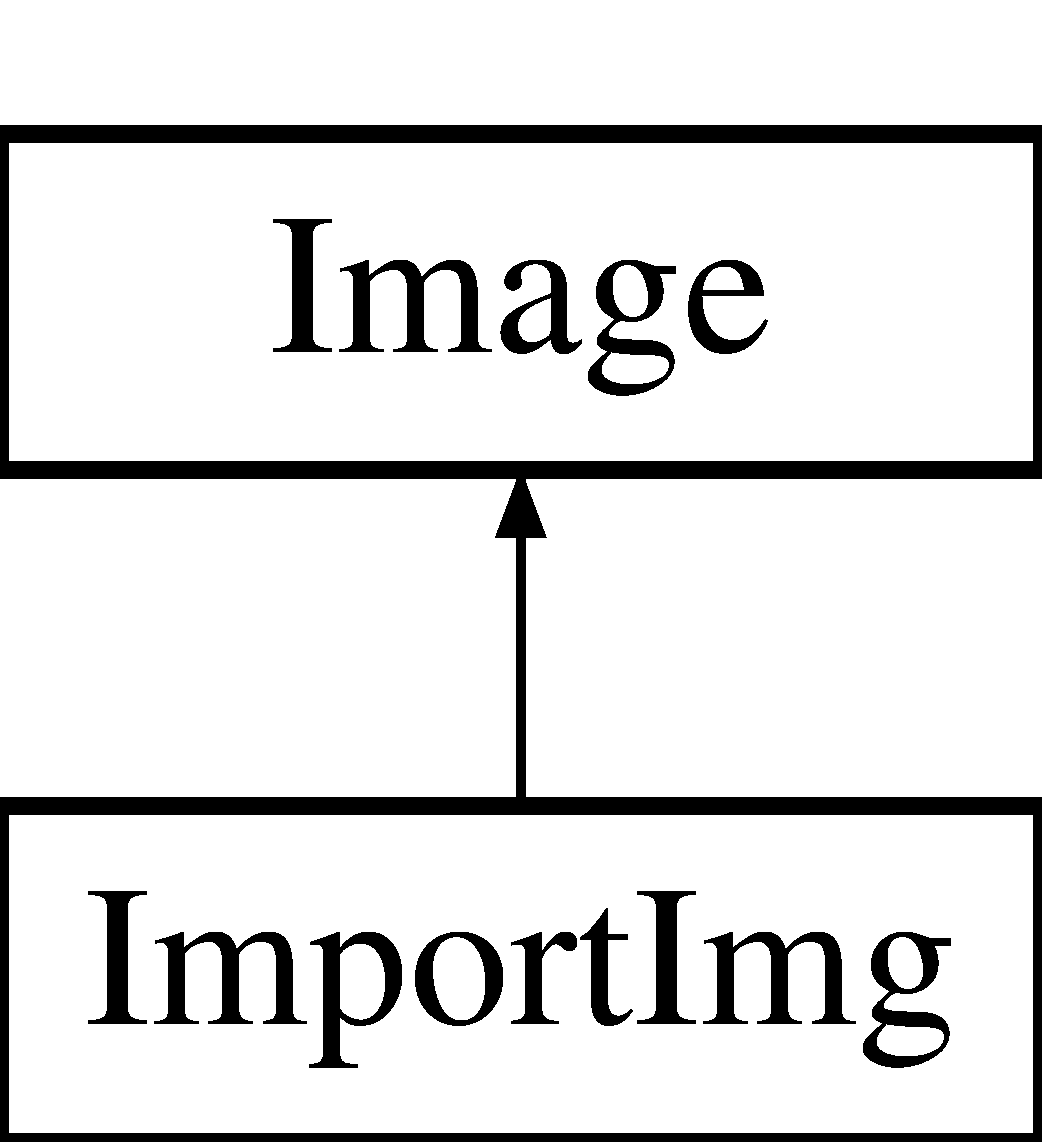
\includegraphics[height=2.000000cm]{classImportImg}
\end{center}
\end{figure}
\subsection*{Public Member Functions}
\begin{DoxyCompactItemize}
\item 
\hyperlink{classImportImg_a888292aaf716935b9e6baddea62af5d8}{Import\-Img} (string file=\char`\"{}\char`\"{})
\item 
\hyperlink{classImportImg_a42a6d3113dfaa5c94fb43360d1641b6f}{Import\-Img} (\hyperlink{classImportImg}{Import\-Img} \&img)
\item 
\hyperlink{classImportImg_adfc26e250764e4388d9aee048a22a673}{Import\-Img} (const \hyperlink{classImportImg}{Import\-Img} \&img)
\item 
\hyperlink{classImportImg_a5b0782a45e30d935067919e69169e809}{$\sim$\-Import\-Img} ()
\begin{DoxyCompactList}\small\item\em Destructor. \end{DoxyCompactList}\end{DoxyCompactItemize}
\subsection*{Private Member Functions}
\begin{DoxyCompactItemize}
\item 
void \hyperlink{classImportImg_a7e1cc1bf176cedb14938519950719fa2}{Create} ()
\begin{DoxyCompactList}\small\item\em Function to create the image. \end{DoxyCompactList}\item 
void \hyperlink{classImportImg_a20bf0509a73e9c08e89518a2ea9a868a}{Import} (string file, string \&img)
\end{DoxyCompactItemize}
\subsection*{Private Attributes}
\begin{DoxyCompactItemize}
\item 
string \hyperlink{classImportImg_a153117d9186b4d7317259ea9dd4c47b1}{file\-Name}
\begin{DoxyCompactList}\small\item\em The file name containing the image contents. \end{DoxyCompactList}\item 
string \hyperlink{classImportImg_a3529487bc41c4ae9a7926b09aec05305}{img\-Str}
\begin{DoxyCompactList}\small\item\em The image in string form. \end{DoxyCompactList}\end{DoxyCompactItemize}
\subsection*{Additional Inherited Members}


\subsection{Detailed Description}
The \hyperlink{classDefaultImg}{Default\-Img} class represents a basic square image made of characters. 

\begin{DoxyAuthor}{Author}
Reid Paulhus 
\end{DoxyAuthor}
\begin{DoxyDate}{Date}
Oct 20, 2017 
\end{DoxyDate}


\subsection{Constructor \& Destructor Documentation}
\hypertarget{classImportImg_a888292aaf716935b9e6baddea62af5d8}{\index{Import\-Img@{Import\-Img}!Import\-Img@{Import\-Img}}
\index{Import\-Img@{Import\-Img}!ImportImg@{Import\-Img}}
\subsubsection[{Import\-Img}]{\setlength{\rightskip}{0pt plus 5cm}Import\-Img\-::\-Import\-Img (
\begin{DoxyParamCaption}
\item[{string}]{file = {\ttfamily \char`\"{}\char`\"{}}}
\end{DoxyParamCaption}
)}}\label{classImportImg_a888292aaf716935b9e6baddea62af5d8}
constructs an \hyperlink{classImage}{Image} object from the given dimensions 
\begin{DoxyParams}[1]{Parameters}
\mbox{\tt in}  & {\em file} & the file path to get the image from\\
\hline
\end{DoxyParams}
Default Constructor 
\begin{DoxyParams}[1]{Parameters}
\mbox{\tt in}  & {\em file} & the masterfile used \\
\hline
\end{DoxyParams}
\hypertarget{classImportImg_a42a6d3113dfaa5c94fb43360d1641b6f}{\index{Import\-Img@{Import\-Img}!Import\-Img@{Import\-Img}}
\index{Import\-Img@{Import\-Img}!ImportImg@{Import\-Img}}
\subsubsection[{Import\-Img}]{\setlength{\rightskip}{0pt plus 5cm}Import\-Img\-::\-Import\-Img (
\begin{DoxyParamCaption}
\item[{{\bf Import\-Img} \&}]{image}
\end{DoxyParamCaption}
)}}\label{classImportImg_a42a6d3113dfaa5c94fb43360d1641b6f}
Copy constructor to duplicate the given image 
\begin{DoxyParams}[1]{Parameters}
\mbox{\tt in}  & {\em img} & the image to copy from\\
\hline
\end{DoxyParams}
Copy constructor 
\begin{DoxyParams}[1]{Parameters}
\mbox{\tt in}  & {\em image} & the image being copied from \\
\hline
\end{DoxyParams}
\hypertarget{classImportImg_adfc26e250764e4388d9aee048a22a673}{\index{Import\-Img@{Import\-Img}!Import\-Img@{Import\-Img}}
\index{Import\-Img@{Import\-Img}!ImportImg@{Import\-Img}}
\subsubsection[{Import\-Img}]{\setlength{\rightskip}{0pt plus 5cm}Import\-Img\-::\-Import\-Img (
\begin{DoxyParamCaption}
\item[{const {\bf Import\-Img} \&}]{image}
\end{DoxyParamCaption}
)}}\label{classImportImg_adfc26e250764e4388d9aee048a22a673}
Copy constructor to duplicate the given image 
\begin{DoxyParams}[1]{Parameters}
\mbox{\tt in}  & {\em img} & the image to copy from\\
\hline
\end{DoxyParams}
Copy constructor 
\begin{DoxyParams}[1]{Parameters}
\mbox{\tt in}  & {\em image} & the image being copied from \\
\hline
\end{DoxyParams}
\hypertarget{classImportImg_a5b0782a45e30d935067919e69169e809}{\index{Import\-Img@{Import\-Img}!$\sim$\-Import\-Img@{$\sim$\-Import\-Img}}
\index{$\sim$\-Import\-Img@{$\sim$\-Import\-Img}!ImportImg@{Import\-Img}}
\subsubsection[{$\sim$\-Import\-Img}]{\setlength{\rightskip}{0pt plus 5cm}Import\-Img\-::$\sim$\-Import\-Img (
\begin{DoxyParamCaption}
{}
\end{DoxyParamCaption}
)}}\label{classImportImg_a5b0782a45e30d935067919e69169e809}


Destructor. 



\subsection{Member Function Documentation}
\hypertarget{classImportImg_a7e1cc1bf176cedb14938519950719fa2}{\index{Import\-Img@{Import\-Img}!Create@{Create}}
\index{Create@{Create}!ImportImg@{Import\-Img}}
\subsubsection[{Create}]{\setlength{\rightskip}{0pt plus 5cm}void Import\-Img\-::\-Create (
\begin{DoxyParamCaption}
{}
\end{DoxyParamCaption}
)\hspace{0.3cm}{\ttfamily [private]}, {\ttfamily [virtual]}}}\label{classImportImg_a7e1cc1bf176cedb14938519950719fa2}


Function to create the image. 

Function that creates an image based on the file name. 

Reimplemented from \hyperlink{classImage_a6bb7dff9e4c4c31b2d63d7b0a330ef89}{Image}.

\hypertarget{classImportImg_a20bf0509a73e9c08e89518a2ea9a868a}{\index{Import\-Img@{Import\-Img}!Import@{Import}}
\index{Import@{Import}!ImportImg@{Import\-Img}}
\subsubsection[{Import}]{\setlength{\rightskip}{0pt plus 5cm}void Import\-Img\-::\-Import (
\begin{DoxyParamCaption}
\item[{string}]{file, }
\item[{string \&}]{img}
\end{DoxyParamCaption}
)\hspace{0.3cm}{\ttfamily [private]}}}\label{classImportImg_a20bf0509a73e9c08e89518a2ea9a868a}
Helper function to append the lines from the file to create an image 
\begin{DoxyParams}[1]{Parameters}
\mbox{\tt in}  & {\em file} & the file that is being accessed \\
\hline
\mbox{\tt in}  & {\em img} & the string containing all the lines that make up the image\\
\hline
\end{DoxyParams}
Function that imports from a file 
\begin{DoxyParams}[1]{Parameters}
\mbox{\tt in}  & {\em file} & the file to be opened \\
\hline
\mbox{\tt in}  & {\em the} & image in string form (can be used for later) \\
\hline
\end{DoxyParams}


\subsection{Member Data Documentation}
\hypertarget{classImportImg_a153117d9186b4d7317259ea9dd4c47b1}{\index{Import\-Img@{Import\-Img}!file\-Name@{file\-Name}}
\index{file\-Name@{file\-Name}!ImportImg@{Import\-Img}}
\subsubsection[{file\-Name}]{\setlength{\rightskip}{0pt plus 5cm}string Import\-Img\-::file\-Name\hspace{0.3cm}{\ttfamily [private]}}}\label{classImportImg_a153117d9186b4d7317259ea9dd4c47b1}


The file name containing the image contents. 

\hypertarget{classImportImg_a3529487bc41c4ae9a7926b09aec05305}{\index{Import\-Img@{Import\-Img}!img\-Str@{img\-Str}}
\index{img\-Str@{img\-Str}!ImportImg@{Import\-Img}}
\subsubsection[{img\-Str}]{\setlength{\rightskip}{0pt plus 5cm}string Import\-Img\-::img\-Str\hspace{0.3cm}{\ttfamily [private]}}}\label{classImportImg_a3529487bc41c4ae9a7926b09aec05305}


The image in string form. 



The documentation for this class was generated from the following files\-:\begin{DoxyCompactItemize}
\item 
/home/rigt2720/\-Kodika/\-Image/\hyperlink{ImportImg_8h}{Import\-Img.\-h}\item 
/home/rigt2720/\-Kodika/\-Image/\hyperlink{ImportImg_8cpp}{Import\-Img.\-cpp}\end{DoxyCompactItemize}

\hypertarget{classInvisiblePotion}{\section{Invisible\-Potion Class Reference}
\label{classInvisiblePotion}\index{Invisible\-Potion@{Invisible\-Potion}}
}


Subclass of \hyperlink{classConsumable}{Consumable} to represent an in game invisibility potion.  




{\ttfamily \#include $<$My\-Consumables.\-h$>$}

Inheritance diagram for Invisible\-Potion\-:\begin{figure}[H]
\begin{center}
\leavevmode
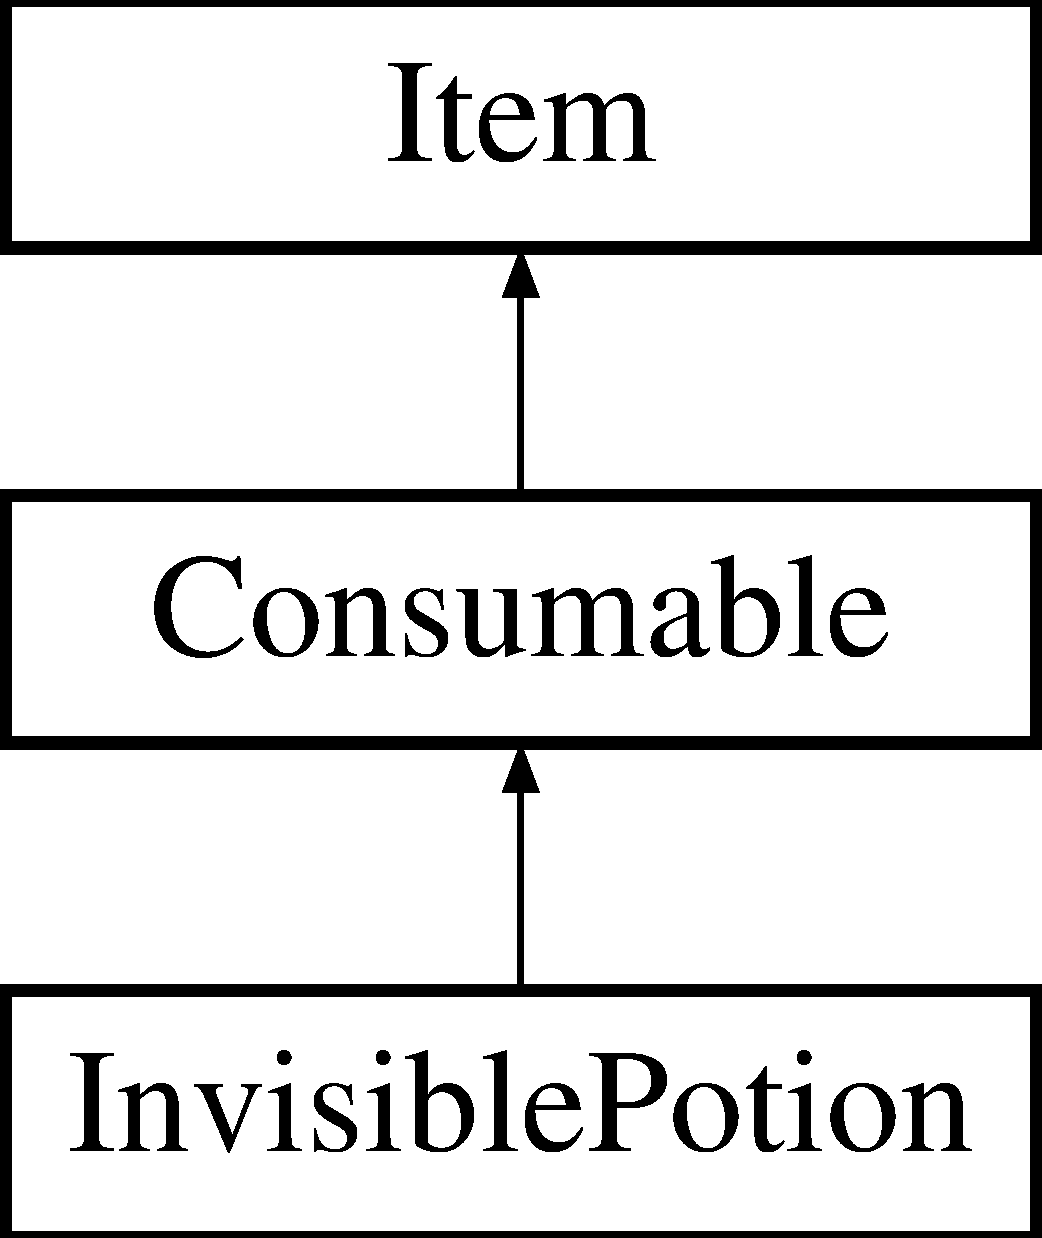
\includegraphics[height=3.000000cm]{classInvisiblePotion}
\end{center}
\end{figure}
\subsection*{Public Member Functions}
\begin{DoxyCompactItemize}
\item 
void \hyperlink{classInvisiblePotion_a183ecf0905d5d6da6f9a59d26fb44d10}{use} (\hyperlink{classCharacter}{Character} $\ast$taget)
\end{DoxyCompactItemize}


\subsection{Detailed Description}
Subclass of \hyperlink{classConsumable}{Consumable} to represent an in game invisibility potion. 

\subsection{Member Function Documentation}
\hypertarget{classInvisiblePotion_a183ecf0905d5d6da6f9a59d26fb44d10}{\index{Invisible\-Potion@{Invisible\-Potion}!use@{use}}
\index{use@{use}!InvisiblePotion@{Invisible\-Potion}}
\subsubsection[{use}]{\setlength{\rightskip}{0pt plus 5cm}void Invisible\-Potion\-::use (
\begin{DoxyParamCaption}
\item[{{\bf Character} $\ast$}]{taget}
\end{DoxyParamCaption}
)}}\label{classInvisiblePotion_a183ecf0905d5d6da6f9a59d26fb44d10}
Defines what happens when the invisibility potion is used param\mbox{[}in\mbox{]} target The \hyperlink{classCharacter}{Character} that the invisibility potion is used on 

The documentation for this class was generated from the following file\-:\begin{DoxyCompactItemize}
\item 
Item/My\-Consumables.\-h\end{DoxyCompactItemize}

\hypertarget{classItem}{\section{Item Class Reference}
\label{classItem}\index{Item@{Item}}
}


This class is an abstract base class to represent items in game.  




{\ttfamily \#include $<$Item.\-h$>$}

Inheritance diagram for Item\-:\begin{figure}[H]
\begin{center}
\leavevmode
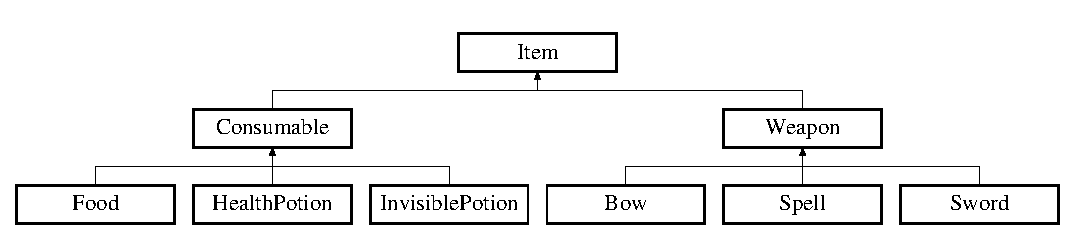
\includegraphics[height=3.000000cm]{classItem}
\end{center}
\end{figure}
\subsection*{Public Member Functions}
\begin{DoxyCompactItemize}
\item 
virtual \hyperlink{classItem_a33cc9c0bc556b5a33a9d0d58d37c602b}{$\sim$\-Item} ()
\begin{DoxyCompactList}\small\item\em Virtual destructor. \end{DoxyCompactList}\item 
\hyperlink{classItem}{Item} $\ast$ \hyperlink{classItem_a7b17a8ea512b73fff57327dbf64e64fc}{Get\-Item} (string item\-Type)
\begin{DoxyCompactList}\small\item\em \hyperlink{classItem}{Item} Factory. \end{DoxyCompactList}\item 
virtual bool \hyperlink{classItem_abd3f52dd7fa25d497f2070e95d44ac03}{Use} (\hyperlink{classCharacter}{Character} $\ast$target)=0
\item 
string \& \hyperlink{classItem_a90ce604a697cdd06ed15c1176f269bcf}{Name} ()
\begin{DoxyCompactList}\small\item\em read or write to name \end{DoxyCompactList}\item 
string \hyperlink{classItem_abbe83003b27f50b343ebfb4b89d73a9b}{Name} () const 
\begin{DoxyCompactList}\small\item\em read name \end{DoxyCompactList}\item 
string \hyperlink{classItem_ac97e1c78a4ea877d9c07774f07dd5fa4}{Name\-Generator} (string file\-Name)
\begin{DoxyCompactList}\small\item\em Creates names for Items. \end{DoxyCompactList}\end{DoxyCompactItemize}
\subsection*{Protected Member Functions}
\begin{DoxyCompactItemize}
\item 
int \hyperlink{classItem_a06cbecc4adca069c237a334998679942}{Random} (unsigned int start, unsigned int end)
\begin{DoxyCompactList}\small\item\em random number generator \end{DoxyCompactList}\end{DoxyCompactItemize}
\subsection*{Protected Attributes}
\begin{DoxyCompactItemize}
\item 
string \hyperlink{classItem_af7a09a8db2072c632d84a992e76408b9}{item\-Name}
\begin{DoxyCompactList}\small\item\em Name of the item. \end{DoxyCompactList}\end{DoxyCompactItemize}


\subsection{Detailed Description}
This class is an abstract base class to represent items in game. 

\subsection{Constructor \& Destructor Documentation}
\hypertarget{classItem_a33cc9c0bc556b5a33a9d0d58d37c602b}{\index{Item@{Item}!$\sim$\-Item@{$\sim$\-Item}}
\index{$\sim$\-Item@{$\sim$\-Item}!Item@{Item}}
\subsubsection[{$\sim$\-Item}]{\setlength{\rightskip}{0pt plus 5cm}virtual Item\-::$\sim$\-Item (
\begin{DoxyParamCaption}
{}
\end{DoxyParamCaption}
)\hspace{0.3cm}{\ttfamily [inline]}, {\ttfamily [virtual]}}}\label{classItem_a33cc9c0bc556b5a33a9d0d58d37c602b}


Virtual destructor. 



\subsection{Member Function Documentation}
\hypertarget{classItem_a7b17a8ea512b73fff57327dbf64e64fc}{\index{Item@{Item}!Get\-Item@{Get\-Item}}
\index{Get\-Item@{Get\-Item}!Item@{Item}}
\subsubsection[{Get\-Item}]{\setlength{\rightskip}{0pt plus 5cm}{\bf Item} $\ast$ Item\-::\-Get\-Item (
\begin{DoxyParamCaption}
\item[{string}]{item\-Type}
\end{DoxyParamCaption}
)}}\label{classItem_a7b17a8ea512b73fff57327dbf64e64fc}


\hyperlink{classItem}{Item} Factory. 

Uses factory design pattern to create items 
\begin{DoxyParams}[1]{Parameters}
\mbox{\tt in}  & {\em item\-Type} & The type of item to be created \\
\hline
\end{DoxyParams}
\begin{DoxyReturn}{Returns}
Pointer to created item 
\end{DoxyReturn}

\begin{DoxyExceptions}{Exceptions}
{\em invalid\-\_\-argument} & Thrown if type does not exist or is not allowed \\
\hline
\end{DoxyExceptions}
\hypertarget{classItem_a90ce604a697cdd06ed15c1176f269bcf}{\index{Item@{Item}!Name@{Name}}
\index{Name@{Name}!Item@{Item}}
\subsubsection[{Name}]{\setlength{\rightskip}{0pt plus 5cm}string \& Item\-::\-Name (
\begin{DoxyParamCaption}
{}
\end{DoxyParamCaption}
)}}\label{classItem_a90ce604a697cdd06ed15c1176f269bcf}


read or write to name 

Allows access to the items name \begin{DoxyReturn}{Returns}
Reference to the name of the item 
\end{DoxyReturn}
\hypertarget{classItem_abbe83003b27f50b343ebfb4b89d73a9b}{\index{Item@{Item}!Name@{Name}}
\index{Name@{Name}!Item@{Item}}
\subsubsection[{Name}]{\setlength{\rightskip}{0pt plus 5cm}string Item\-::\-Name (
\begin{DoxyParamCaption}
{}
\end{DoxyParamCaption}
) const}}\label{classItem_abbe83003b27f50b343ebfb4b89d73a9b}


read name 

Gives the name of the item without allowing chages \begin{DoxyReturn}{Returns}
Name of the item 
\end{DoxyReturn}
\hypertarget{classItem_ac97e1c78a4ea877d9c07774f07dd5fa4}{\index{Item@{Item}!Name\-Generator@{Name\-Generator}}
\index{Name\-Generator@{Name\-Generator}!Item@{Item}}
\subsubsection[{Name\-Generator}]{\setlength{\rightskip}{0pt plus 5cm}string Item\-::\-Name\-Generator (
\begin{DoxyParamCaption}
\item[{string}]{file\-Name}
\end{DoxyParamCaption}
)}}\label{classItem_ac97e1c78a4ea877d9c07774f07dd5fa4}


Creates names for Items. 

Generates adjectives to add to \hyperlink{classItem}{Item} names 
\begin{DoxyParams}[1]{Parameters}
\mbox{\tt in}  & {\em file\-Name} & the file that the names comme from \\
\hline
\end{DoxyParams}
\begin{DoxyReturn}{Returns}
Adjective generated and to be used 
\end{DoxyReturn}

\begin{DoxyExceptions}{Exceptions}
{\em runtime\-\_\-error} & Thrown if source file has no names \\
\hline
\end{DoxyExceptions}
\hypertarget{classItem_a06cbecc4adca069c237a334998679942}{\index{Item@{Item}!Random@{Random}}
\index{Random@{Random}!Item@{Item}}
\subsubsection[{Random}]{\setlength{\rightskip}{0pt plus 5cm}int Item\-::\-Random (
\begin{DoxyParamCaption}
\item[{unsigned int}]{start, }
\item[{unsigned int}]{end}
\end{DoxyParamCaption}
)\hspace{0.3cm}{\ttfamily [protected]}}}\label{classItem_a06cbecc4adca069c237a334998679942}


random number generator 

Helper function to generate random positive numbers \begin{DoxyReturn}{Returns}
Random number between start and end 
\end{DoxyReturn}
\hypertarget{classItem_abd3f52dd7fa25d497f2070e95d44ac03}{\index{Item@{Item}!Use@{Use}}
\index{Use@{Use}!Item@{Item}}
\subsubsection[{Use}]{\setlength{\rightskip}{0pt plus 5cm}virtual bool Item\-::\-Use (
\begin{DoxyParamCaption}
\item[{{\bf Character} $\ast$}]{target}
\end{DoxyParamCaption}
)\hspace{0.3cm}{\ttfamily [pure virtual]}}}\label{classItem_abd3f52dd7fa25d497f2070e95d44ac03}
Pure Virtual funtion that forces all subclasses to define how to use themselves 
\begin{DoxyParams}[1]{Parameters}
\mbox{\tt in}  & {\em target} & The \hyperlink{classCharacter}{Character} the item is being used on \\
\hline
\end{DoxyParams}
\begin{DoxyReturn}{Returns}
true if use was successfull 
\end{DoxyReturn}


Implemented in \hyperlink{classSpell_a22680a625dce4f3a85421c4763930b57}{Spell}, \hyperlink{classFood_a03ce09da13a4d8b9bb7a789a3ede42be}{Food}, \hyperlink{classBow_a07d98049b83e0f21ccbef29c7294bde7}{Bow}, \hyperlink{classHealthPotion_a6fee598a4d80425364c72da18b883615}{Health\-Potion}, and \hyperlink{classSword_a95e6215b5a27b6d2edc5c59e2a2a408b}{Sword}.



\subsection{Member Data Documentation}
\hypertarget{classItem_af7a09a8db2072c632d84a992e76408b9}{\index{Item@{Item}!item\-Name@{item\-Name}}
\index{item\-Name@{item\-Name}!Item@{Item}}
\subsubsection[{item\-Name}]{\setlength{\rightskip}{0pt plus 5cm}string Item\-::item\-Name\hspace{0.3cm}{\ttfamily [protected]}}}\label{classItem_af7a09a8db2072c632d84a992e76408b9}


Name of the item. 



The documentation for this class was generated from the following files\-:\begin{DoxyCompactItemize}
\item 
/home/rigt2720/\-Kodika/\-Item/\hyperlink{Item_8h}{Item.\-h}\item 
/home/rigt2720/\-Kodika/\-Item/\hyperlink{Item_8cpp}{Item.\-cpp}\end{DoxyCompactItemize}

\hypertarget{classMainMenu}{\section{Main\-Menu Class Reference}
\label{classMainMenu}\index{Main\-Menu@{Main\-Menu}}
}


This is the menu for the player to use when they are either not in the game or have died and need to restart or quit.  




{\ttfamily \#include $<$Main\-Menu.\-h$>$}

Inheritance diagram for Main\-Menu\-:\begin{figure}[H]
\begin{center}
\leavevmode
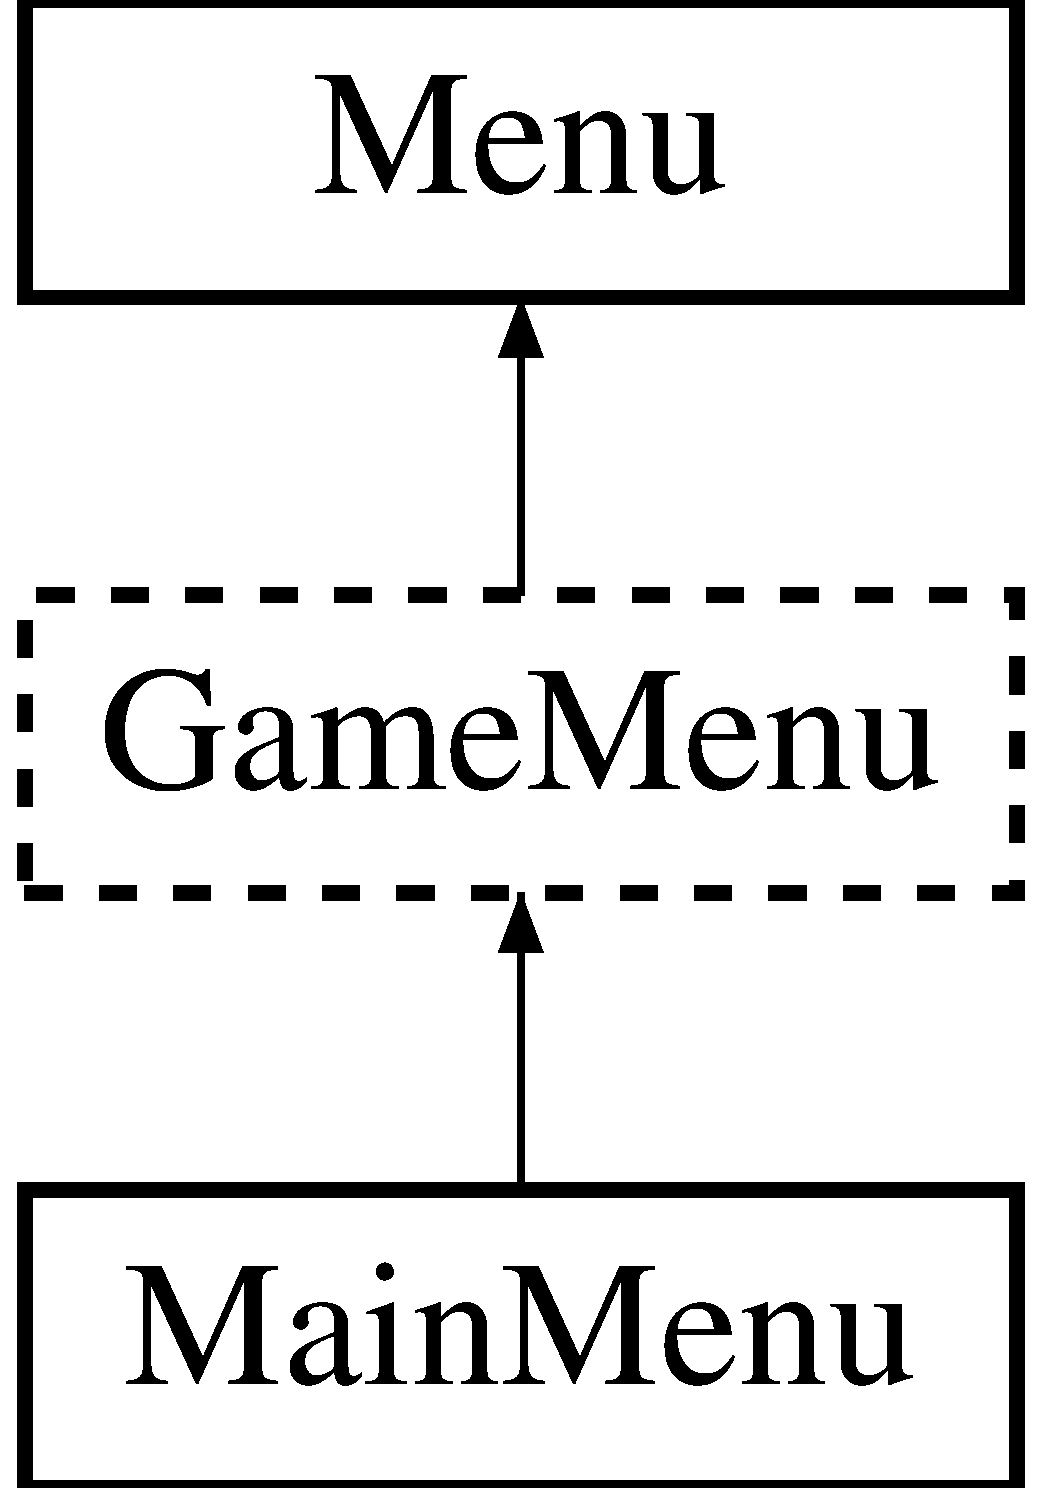
\includegraphics[height=3.000000cm]{classMainMenu}
\end{center}
\end{figure}
\subsection*{Public Member Functions}
\begin{DoxyCompactItemize}
\item 
\hyperlink{classMainMenu_aa626a8f5895b449a1d23f5be235210aa}{Main\-Menu} (int height=33)
\begin{DoxyCompactList}\small\item\em This is the default constructor. \end{DoxyCompactList}\item 
virtual void \hyperlink{classMainMenu_a44ab04810a68d7ddf3843464573b7967}{Set\-Options} (int row, int col, int space)
\item 
virtual void \hyperlink{classMainMenu_a85703c73c1bcc9be2144b1cbe413328e}{Handle\-Input} (istream \&is)
\end{DoxyCompactItemize}
\subsection*{Private Attributes}
\begin{DoxyCompactItemize}
\item 
\hyperlink{classMenu}{Menu} $\ast$ \hyperlink{classMainMenu_ae7d51673d2212c49550307dff79f6aba}{menu}
\end{DoxyCompactItemize}
\subsection*{Additional Inherited Members}


\subsection{Detailed Description}
This is the menu for the player to use when they are either not in the game or have died and need to restart or quit. 

\subsection{Constructor \& Destructor Documentation}
\hypertarget{classMainMenu_aa626a8f5895b449a1d23f5be235210aa}{\index{Main\-Menu@{Main\-Menu}!Main\-Menu@{Main\-Menu}}
\index{Main\-Menu@{Main\-Menu}!MainMenu@{Main\-Menu}}
\subsubsection[{Main\-Menu}]{\setlength{\rightskip}{0pt plus 5cm}Main\-Menu\-::\-Main\-Menu (
\begin{DoxyParamCaption}
\item[{int}]{height = {\ttfamily 33}}
\end{DoxyParamCaption}
)}}\label{classMainMenu_aa626a8f5895b449a1d23f5be235210aa}


This is the default constructor. 



\subsection{Member Function Documentation}
\hypertarget{classMainMenu_a85703c73c1bcc9be2144b1cbe413328e}{\index{Main\-Menu@{Main\-Menu}!Handle\-Input@{Handle\-Input}}
\index{Handle\-Input@{Handle\-Input}!MainMenu@{Main\-Menu}}
\subsubsection[{Handle\-Input}]{\setlength{\rightskip}{0pt plus 5cm}void Main\-Menu\-::\-Handle\-Input (
\begin{DoxyParamCaption}
\item[{istream \&}]{is}
\end{DoxyParamCaption}
)\hspace{0.3cm}{\ttfamily [virtual]}}}\label{classMainMenu_a85703c73c1bcc9be2144b1cbe413328e}
This function handles the input for the menu options. 
\begin{DoxyParams}[1]{Parameters}
\mbox{\tt in,out}  & {\em is} & The in-\/stream operator to read the input. \\
\hline
\end{DoxyParams}


Implements \hyperlink{classGameMenu_a02ba09feedece5773f44ba865ccffb42}{Game\-Menu}.

\hypertarget{classMainMenu_a44ab04810a68d7ddf3843464573b7967}{\index{Main\-Menu@{Main\-Menu}!Set\-Options@{Set\-Options}}
\index{Set\-Options@{Set\-Options}!MainMenu@{Main\-Menu}}
\subsubsection[{Set\-Options}]{\setlength{\rightskip}{0pt plus 5cm}void Main\-Menu\-::\-Set\-Options (
\begin{DoxyParamCaption}
\item[{int}]{row, }
\item[{int}]{col, }
\item[{int}]{space}
\end{DoxyParamCaption}
)\hspace{0.3cm}{\ttfamily [virtual]}}}\label{classMainMenu_a44ab04810a68d7ddf3843464573b7967}
This function sets the specific options for the \hyperlink{classMenu}{Menu} type. 
\begin{DoxyParams}[1]{Parameters}
\mbox{\tt in}  & {\em Options\-List} & A map of all the options for the current menu. Each option has a unique key to make input easier. \\
\hline
\mbox{\tt in}  & {\em type} & This denotes the type of menu to display. \\
\hline
\end{DoxyParams}


Implements \hyperlink{classGameMenu_ac32ff465c5a4f30979e8851fa21cb230}{Game\-Menu}.



\subsection{Member Data Documentation}
\hypertarget{classMainMenu_ae7d51673d2212c49550307dff79f6aba}{\index{Main\-Menu@{Main\-Menu}!menu@{menu}}
\index{menu@{menu}!MainMenu@{Main\-Menu}}
\subsubsection[{menu}]{\setlength{\rightskip}{0pt plus 5cm}{\bf Menu}$\ast$ Main\-Menu\-::menu\hspace{0.3cm}{\ttfamily [private]}}}\label{classMainMenu_ae7d51673d2212c49550307dff79f6aba}


The documentation for this class was generated from the following files\-:\begin{DoxyCompactItemize}
\item 
/home/rigt2720/\-Kodika/\-Menu/\hyperlink{MainMenu_8h}{Main\-Menu.\-h}\item 
/home/rigt2720/\-Kodika/\-Menu/\hyperlink{MainMenu_8cpp}{Main\-Menu.\-cpp}\end{DoxyCompactItemize}

\hypertarget{classMainState}{\section{Main\-State Class Reference}
\label{classMainState}\index{Main\-State@{Main\-State}}
}


This is the state of the game when the game is either not yet started or the game has ended. Derived from \hyperlink{classGameState}{Game\-State}.  




{\ttfamily \#include $<$Main\-State.\-h$>$}

Inheritance diagram for Main\-State\-:\begin{figure}[H]
\begin{center}
\leavevmode
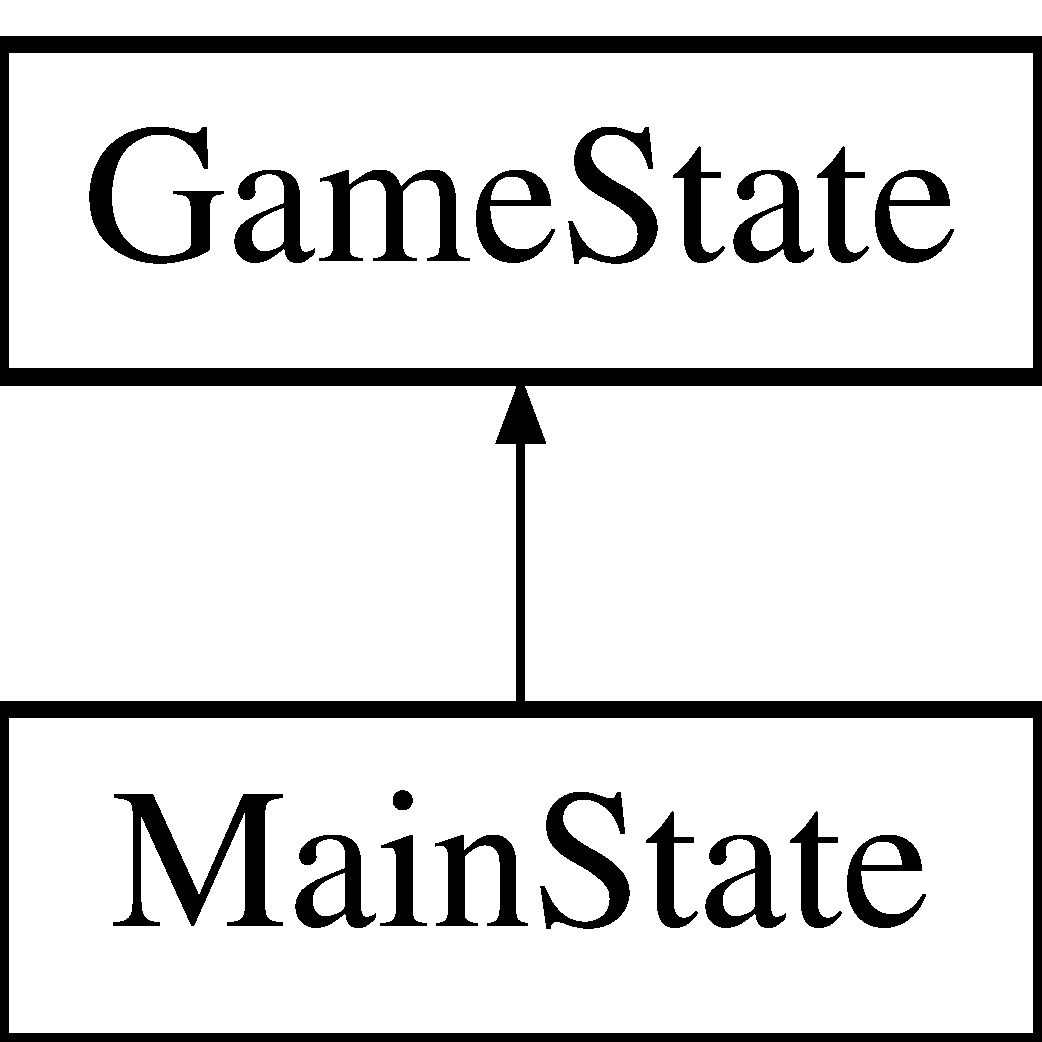
\includegraphics[height=2.000000cm]{classMainState}
\end{center}
\end{figure}
\subsection*{Public Member Functions}
\begin{DoxyCompactItemize}
\item 
\hyperlink{classMainState_afc29557ba046813d1bff4aea2501b7f1}{Main\-State} ()
\begin{DoxyCompactList}\small\item\em Default constructor. \end{DoxyCompactList}\item 
void \hyperlink{classMainState_ac01eced9d617c8c8f5382a9aa96adb45}{Set} ()
\begin{DoxyCompactList}\small\item\em Sets the layout of the game. \end{DoxyCompactList}\item 
void \hyperlink{classMainState_a23233e859905d025cfc031a12977a844}{Get} ()
\begin{DoxyCompactList}\small\item\em Outputs the set layout. \end{DoxyCompactList}\end{DoxyCompactItemize}
\subsection*{Additional Inherited Members}


\subsection{Detailed Description}
This is the state of the game when the game is either not yet started or the game has ended. Derived from \hyperlink{classGameState}{Game\-State}. 

\begin{DoxyDate}{Date}
21/10/2017 
\end{DoxyDate}
\begin{DoxyAuthor}{Author}
Tomas Rigaux
\end{DoxyAuthor}
This class is derived from the \hyperlink{classGameState}{Game\-State} abstract class. It sets the state of the game. 

\subsection{Constructor \& Destructor Documentation}
\hypertarget{classMainState_afc29557ba046813d1bff4aea2501b7f1}{\index{Main\-State@{Main\-State}!Main\-State@{Main\-State}}
\index{Main\-State@{Main\-State}!MainState@{Main\-State}}
\subsubsection[{Main\-State}]{\setlength{\rightskip}{0pt plus 5cm}Main\-State\-::\-Main\-State (
\begin{DoxyParamCaption}
{}
\end{DoxyParamCaption}
)}}\label{classMainState_afc29557ba046813d1bff4aea2501b7f1}


Default constructor. 



\subsection{Member Function Documentation}
\hypertarget{classMainState_a23233e859905d025cfc031a12977a844}{\index{Main\-State@{Main\-State}!Get@{Get}}
\index{Get@{Get}!MainState@{Main\-State}}
\subsubsection[{Get}]{\setlength{\rightskip}{0pt plus 5cm}void Main\-State\-::\-Get (
\begin{DoxyParamCaption}
{}
\end{DoxyParamCaption}
)\hspace{0.3cm}{\ttfamily [virtual]}}}\label{classMainState_a23233e859905d025cfc031a12977a844}


Outputs the set layout. 



Implements \hyperlink{classGameState_a4283cb3aa5637d4815d64272843a0625}{Game\-State}.

\hypertarget{classMainState_ac01eced9d617c8c8f5382a9aa96adb45}{\index{Main\-State@{Main\-State}!Set@{Set}}
\index{Set@{Set}!MainState@{Main\-State}}
\subsubsection[{Set}]{\setlength{\rightskip}{0pt plus 5cm}void Main\-State\-::\-Set (
\begin{DoxyParamCaption}
{}
\end{DoxyParamCaption}
)\hspace{0.3cm}{\ttfamily [virtual]}}}\label{classMainState_ac01eced9d617c8c8f5382a9aa96adb45}


Sets the layout of the game. 



Implements \hyperlink{classGameState_af22e9a43999f99b784a35fab85cd9208}{Game\-State}.



The documentation for this class was generated from the following files\-:\begin{DoxyCompactItemize}
\item 
/home/rigt2720/\-Kodika/\-Game\-State/\hyperlink{MainState_8h}{Main\-State.\-h}\item 
/home/rigt2720/\-Kodika/\-Game\-State/\hyperlink{MainState_8cpp}{Main\-State.\-cpp}\end{DoxyCompactItemize}

\hypertarget{classMemoryMatch}{\section{Memory\-Match Class Reference}
\label{classMemoryMatch}\index{Memory\-Match@{Memory\-Match}}
}


This class contains the mini-\/game/puzzle Memory Match.  




{\ttfamily \#include $<$Memory\-Match.\-h$>$}

Inheritance diagram for Memory\-Match\-:\begin{figure}[H]
\begin{center}
\leavevmode
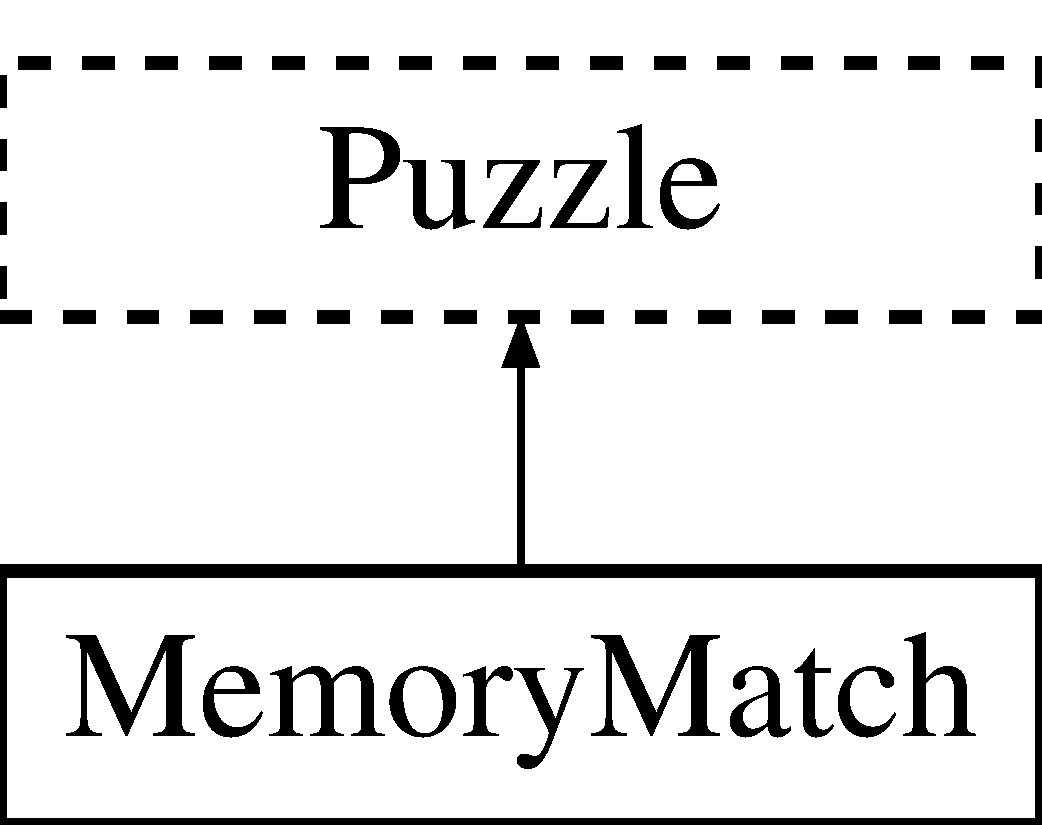
\includegraphics[height=2.000000cm]{classMemoryMatch}
\end{center}
\end{figure}
\subsection*{Public Member Functions}
\begin{DoxyCompactItemize}
\item 
\hyperlink{classMemoryMatch_a7221a0b7d33bf079df51c1f7f52aa2dd}{Memory\-Match} ()
\begin{DoxyCompactList}\small\item\em Default constructor for \hyperlink{classMemoryMatch}{Memory\-Match}, sets height to\-: and width to\-: \end{DoxyCompactList}\item 
virtual \hyperlink{classMemoryMatch_a1b2cf5418b2b26e21b4fd12d880e79b7}{$\sim$\-Memory\-Match} ()
\begin{DoxyCompactList}\small\item\em Deconstructor. \end{DoxyCompactList}\item 
void \hyperlink{classMemoryMatch_a090950f764dee0b982ea254075d3667c}{Run\-Game} (\hyperlink{classCharacter}{Character} $\ast$player)
\end{DoxyCompactItemize}
\subsection*{Private Member Functions}
\begin{DoxyCompactItemize}
\item 
void \hyperlink{classMemoryMatch_a62548d6cf028d372c08cc01a0693edb2}{Set\-Options\-In\-Menu} ()
\begin{DoxyCompactList}\small\item\em Sends the menu class the options for the player to select. \end{DoxyCompactList}\item 
void \hyperlink{classMemoryMatch_a1e3b9172bdd0fb69f0360bb28acee65c}{Board\-Setup} ()
\begin{DoxyCompactList}\small\item\em Sets the board up for the beginning of the game, placing them in screen. \end{DoxyCompactList}\item 
void \hyperlink{classMemoryMatch_a026870bd184e56fc576c1ec85f64b487}{Set\-Inputs} (int \&X1, int \&Y1, int \&X2, int \&Y2, \hyperlink{classMemoryMenu}{Memory\-Menu} \&menu)
\item 
bool \hyperlink{classMemoryMatch_a64f64d28f47e59f3303addf70ca136e2}{Check\-Input} (int x1, int y1, int x2, int y2)
\begin{DoxyCompactList}\small\item\em Checks the semantics of the players selection. \end{DoxyCompactList}\item 
bool \hyperlink{classMemoryMatch_a8d0683346a26c1d00c818e9b75b5a412}{Is\-Input\-Valid} (int input)
\item 
bool \hyperlink{classMemoryMatch_ae5f190c71bc1a63ec95eab6fd8a3c2c7}{Valid\-Move} (int input\-X1, int input\-Y1, int input\-X2, int input\-Y2)
\item 
void \hyperlink{classMemoryMatch_a68e81f3e7ed13385f430da0bc938d7e9}{Move\-Piece} (int input\-X1, int input\-Y1, int input\-X2, int input\-Y2)
\item 
bool \hyperlink{classMemoryMatch_a7a83e4a378bb74a729d495d9a8896248}{Match\-Check} (int input\-X1, int input\-Y1, int input\-X2, int input\-Y2)
\item 
void \hyperlink{classMemoryMatch_a1c958b2c366188c2c603c562b3f2f878}{Win\-Check} ()
\item 
void \hyperlink{classMemoryMatch_a61158d799b281be3607860233899b405}{Randomly\-Insert\-Into\-Table} (char symbol)
\begin{DoxyCompactList}\small\item\em randomly puts pairs into the table \end{DoxyCompactList}\item 
void \hyperlink{classMemoryMatch_a9ea522ae206345fc5a6d730ed7ff4adc}{Flip\-Two\-Chars} (int input\-X, int input\-Y)
\item 
int \hyperlink{classMemoryMatch_ae684d58439ac7d7ca9e6dcd8b1c1f977}{Convert\-Char\-To\-Index} (char input)
\item 
int \hyperlink{classMemoryMatch_a0543038015f3bbd9db9e9a235cf12579}{Random\-Number} (int n)
\begin{DoxyCompactList}\small\item\em Returns a random number between 0 and n-\/1. \end{DoxyCompactList}\item 
void \hyperlink{classMemoryMatch_a6d4c54b56ee4f5b4df36b7767e07ebd5}{Save\-Board\-To\-Screen} ()
\item 
void \hyperlink{classMemoryMatch_a56bf6c64798545d880f6d061464ae5a2}{Peek\-At\-Board} (int length\-In\-Seconds)
\begin{DoxyCompactList}\small\item\em Flips two squares and outputs it for 3 seconds then flips it back. \end{DoxyCompactList}\item 
void \hyperlink{classMemoryMatch_a5a3232cd99dddddc6af5d5dc050087f7}{End\-Game\-Prompt} ()
\item 
void \hyperlink{classMemoryMatch_acfc3d904747668225bd52a508d9dcae6}{Second\-Delay} (int seconds)
\begin{DoxyCompactList}\small\item\em Causes a \char`\"{}seconds\char`\"{} delay in the program process. \end{DoxyCompactList}\item 
void \hyperlink{classMemoryMatch_ae78665422f8d46d0c4639916f494845c}{Peek} (int input\-X1, int input\-Y1, int input\-X2, int input\-Y2)
\begin{DoxyCompactList}\small\item\em Flips two squares and outputs it for 3 seconds then flips it back. \end{DoxyCompactList}\item 
bool \hyperlink{classMemoryMatch_a2cdc3fbc35524564a651e3cc1d5d03df}{Is\-Odd} (int n)
\begin{DoxyCompactList}\small\item\em Returns true if n is odd, false if even. \end{DoxyCompactList}\item 
bool \hyperlink{classMemoryMatch_a7f3998ff0f59a063a493156c2d00eca2}{Is\-In\-Used\-Pairs} (char symbol)
\begin{DoxyCompactList}\small\item\em Checks if the symbol has been used in the random board already. \end{DoxyCompactList}\item 
bool \hyperlink{classMemoryMatch_acf4047dc2a34d4045a6a240253cb5600}{Is\-Char\-Already\-Matched} (int input\-X, int input\-Y)
\begin{DoxyCompactList}\small\item\em Returns true if char has a true value in the match\-Vector, false otherwise. \end{DoxyCompactList}\end{DoxyCompactItemize}
\subsection*{Private Attributes}
\begin{DoxyCompactItemize}
\item 
\hyperlink{classScreen}{Screen} \hyperlink{classMemoryMatch_a78399975fec5fea7b2102449a4536fcd}{Memory\-Match\-Screen}
\item 
std\-::vector$<$ vector$<$ char $>$ $>$ \hyperlink{classMemoryMatch_af2437cf6ce06147e64feb7dca23715e7}{char\-Table}
\begin{DoxyCompactList}\small\item\em The vector which holds the char values of the table to be matched. \end{DoxyCompactList}\item 
std\-::vector$<$ vector$<$ int $>$ $>$ \hyperlink{classMemoryMatch_a87ee5474b348c72d91a359e1bbbe2e10}{match\-Vector}
\item 
std\-::vector$<$ char $>$ \hyperlink{classMemoryMatch_a80336b0b989152fed590a6fa755197bc}{pairs\-Of\-Chars\-Vector}
\begin{DoxyCompactList}\small\item\em Vector containing symbols to be randomly inserted on the screen at start. \end{DoxyCompactList}\item 
std\-::vector$<$ char $>$ \hyperlink{classMemoryMatch_adcb66679aaceb1414fe023d065863d2f}{used\-Pairs}
\begin{DoxyCompactList}\small\item\em Vector containing all pairs that have already been matched up. \end{DoxyCompactList}\item 
int \hyperlink{classMemoryMatch_aae0a9e51558d70e671fa64aa246de499}{board\-Size}
\begin{DoxyCompactList}\small\item\em dimensions for the gameboard \end{DoxyCompactList}\end{DoxyCompactItemize}
\subsection*{Additional Inherited Members}


\subsection{Detailed Description}
This class contains the mini-\/game/puzzle Memory Match. 

\begin{DoxyAuthor}{Author}
Tyler Siwy 
\end{DoxyAuthor}
\begin{DoxyDate}{Date}
Oct 20, 2017 
\end{DoxyDate}


\subsection{Constructor \& Destructor Documentation}
\hypertarget{classMemoryMatch_a7221a0b7d33bf079df51c1f7f52aa2dd}{\index{Memory\-Match@{Memory\-Match}!Memory\-Match@{Memory\-Match}}
\index{Memory\-Match@{Memory\-Match}!MemoryMatch@{Memory\-Match}}
\subsubsection[{Memory\-Match}]{\setlength{\rightskip}{0pt plus 5cm}Memory\-Match\-::\-Memory\-Match (
\begin{DoxyParamCaption}
{}
\end{DoxyParamCaption}
)}}\label{classMemoryMatch_a7221a0b7d33bf079df51c1f7f52aa2dd}


Default constructor for \hyperlink{classMemoryMatch}{Memory\-Match}, sets height to\-: and width to\-: 

memory\-\_\-match.\-cpp \begin{DoxyAuthor}{Author}
Tyler Siwy C\-P\-S\-C 2720-\/\-Howard Cheng-\/\-Dungeon Dweller 
\end{DoxyAuthor}
\hypertarget{classMemoryMatch_a1b2cf5418b2b26e21b4fd12d880e79b7}{\index{Memory\-Match@{Memory\-Match}!$\sim$\-Memory\-Match@{$\sim$\-Memory\-Match}}
\index{$\sim$\-Memory\-Match@{$\sim$\-Memory\-Match}!MemoryMatch@{Memory\-Match}}
\subsubsection[{$\sim$\-Memory\-Match}]{\setlength{\rightskip}{0pt plus 5cm}Memory\-Match\-::$\sim$\-Memory\-Match (
\begin{DoxyParamCaption}
{}
\end{DoxyParamCaption}
)\hspace{0.3cm}{\ttfamily [virtual]}}}\label{classMemoryMatch_a1b2cf5418b2b26e21b4fd12d880e79b7}


Deconstructor. 



\subsection{Member Function Documentation}
\hypertarget{classMemoryMatch_a1e3b9172bdd0fb69f0360bb28acee65c}{\index{Memory\-Match@{Memory\-Match}!Board\-Setup@{Board\-Setup}}
\index{Board\-Setup@{Board\-Setup}!MemoryMatch@{Memory\-Match}}
\subsubsection[{Board\-Setup}]{\setlength{\rightskip}{0pt plus 5cm}void Memory\-Match\-::\-Board\-Setup (
\begin{DoxyParamCaption}
{}
\end{DoxyParamCaption}
)\hspace{0.3cm}{\ttfamily [private]}}}\label{classMemoryMatch_a1e3b9172bdd0fb69f0360bb28acee65c}


Sets the board up for the beginning of the game, placing them in screen. 

Setting up the match-\/true/false value vector for win checking/error checking

Try random pairs until the table has been filled in a random order

half of the area of the board since there are pairs so /2

Chose a random pair from the table of possible pairs

If we haven't used any pair yet. Insert right away

Else check if we have used it before, if yes, try another pair \hypertarget{classMemoryMatch_a64f64d28f47e59f3303addf70ca136e2}{\index{Memory\-Match@{Memory\-Match}!Check\-Input@{Check\-Input}}
\index{Check\-Input@{Check\-Input}!MemoryMatch@{Memory\-Match}}
\subsubsection[{Check\-Input}]{\setlength{\rightskip}{0pt plus 5cm}bool Memory\-Match\-::\-Check\-Input (
\begin{DoxyParamCaption}
\item[{int}]{x1, }
\item[{int}]{y1, }
\item[{int}]{x2, }
\item[{int}]{y2}
\end{DoxyParamCaption}
)\hspace{0.3cm}{\ttfamily [private]}}}\label{classMemoryMatch_a64f64d28f47e59f3303addf70ca136e2}


Checks the semantics of the players selection. 

\hypertarget{classMemoryMatch_ae684d58439ac7d7ca9e6dcd8b1c1f977}{\index{Memory\-Match@{Memory\-Match}!Convert\-Char\-To\-Index@{Convert\-Char\-To\-Index}}
\index{Convert\-Char\-To\-Index@{Convert\-Char\-To\-Index}!MemoryMatch@{Memory\-Match}}
\subsubsection[{Convert\-Char\-To\-Index}]{\setlength{\rightskip}{0pt plus 5cm}int Memory\-Match\-::\-Convert\-Char\-To\-Index (
\begin{DoxyParamCaption}
\item[{char}]{input}
\end{DoxyParamCaption}
)\hspace{0.3cm}{\ttfamily [private]}}}\label{classMemoryMatch_ae684d58439ac7d7ca9e6dcd8b1c1f977}
\hypertarget{classMemoryMatch_a5a3232cd99dddddc6af5d5dc050087f7}{\index{Memory\-Match@{Memory\-Match}!End\-Game\-Prompt@{End\-Game\-Prompt}}
\index{End\-Game\-Prompt@{End\-Game\-Prompt}!MemoryMatch@{Memory\-Match}}
\subsubsection[{End\-Game\-Prompt}]{\setlength{\rightskip}{0pt plus 5cm}void Memory\-Match\-::\-End\-Game\-Prompt (
\begin{DoxyParamCaption}
{}
\end{DoxyParamCaption}
)\hspace{0.3cm}{\ttfamily [private]}}}\label{classMemoryMatch_a5a3232cd99dddddc6af5d5dc050087f7}
\hypertarget{classMemoryMatch_a9ea522ae206345fc5a6d730ed7ff4adc}{\index{Memory\-Match@{Memory\-Match}!Flip\-Two\-Chars@{Flip\-Two\-Chars}}
\index{Flip\-Two\-Chars@{Flip\-Two\-Chars}!MemoryMatch@{Memory\-Match}}
\subsubsection[{Flip\-Two\-Chars}]{\setlength{\rightskip}{0pt plus 5cm}void Memory\-Match\-::\-Flip\-Two\-Chars (
\begin{DoxyParamCaption}
\item[{int}]{input\-X, }
\item[{int}]{input\-Y}
\end{DoxyParamCaption}
)\hspace{0.3cm}{\ttfamily [private]}}}\label{classMemoryMatch_a9ea522ae206345fc5a6d730ed7ff4adc}
Flips the char stored at the inputted coordinates on chartable and sets them on the screen. top left coordinate of the game board on the screen

Symbol to be displayed

Display the first symbol \hypertarget{classMemoryMatch_acf4047dc2a34d4045a6a240253cb5600}{\index{Memory\-Match@{Memory\-Match}!Is\-Char\-Already\-Matched@{Is\-Char\-Already\-Matched}}
\index{Is\-Char\-Already\-Matched@{Is\-Char\-Already\-Matched}!MemoryMatch@{Memory\-Match}}
\subsubsection[{Is\-Char\-Already\-Matched}]{\setlength{\rightskip}{0pt plus 5cm}bool Memory\-Match\-::\-Is\-Char\-Already\-Matched (
\begin{DoxyParamCaption}
\item[{int}]{input\-X, }
\item[{int}]{input\-Y}
\end{DoxyParamCaption}
)\hspace{0.3cm}{\ttfamily [private]}}}\label{classMemoryMatch_acf4047dc2a34d4045a6a240253cb5600}


Returns true if char has a true value in the match\-Vector, false otherwise. 

\hypertarget{classMemoryMatch_a8d0683346a26c1d00c818e9b75b5a412}{\index{Memory\-Match@{Memory\-Match}!Is\-Input\-Valid@{Is\-Input\-Valid}}
\index{Is\-Input\-Valid@{Is\-Input\-Valid}!MemoryMatch@{Memory\-Match}}
\subsubsection[{Is\-Input\-Valid}]{\setlength{\rightskip}{0pt plus 5cm}bool Memory\-Match\-::\-Is\-Input\-Valid (
\begin{DoxyParamCaption}
\item[{int}]{input}
\end{DoxyParamCaption}
)\hspace{0.3cm}{\ttfamily [private]}}}\label{classMemoryMatch_a8d0683346a26c1d00c818e9b75b5a412}
\hypertarget{classMemoryMatch_a7f3998ff0f59a063a493156c2d00eca2}{\index{Memory\-Match@{Memory\-Match}!Is\-In\-Used\-Pairs@{Is\-In\-Used\-Pairs}}
\index{Is\-In\-Used\-Pairs@{Is\-In\-Used\-Pairs}!MemoryMatch@{Memory\-Match}}
\subsubsection[{Is\-In\-Used\-Pairs}]{\setlength{\rightskip}{0pt plus 5cm}bool Memory\-Match\-::\-Is\-In\-Used\-Pairs (
\begin{DoxyParamCaption}
\item[{char}]{symbol}
\end{DoxyParamCaption}
)\hspace{0.3cm}{\ttfamily [private]}}}\label{classMemoryMatch_a7f3998ff0f59a063a493156c2d00eca2}


Checks if the symbol has been used in the random board already. 

\hypertarget{classMemoryMatch_a2cdc3fbc35524564a651e3cc1d5d03df}{\index{Memory\-Match@{Memory\-Match}!Is\-Odd@{Is\-Odd}}
\index{Is\-Odd@{Is\-Odd}!MemoryMatch@{Memory\-Match}}
\subsubsection[{Is\-Odd}]{\setlength{\rightskip}{0pt plus 5cm}bool Memory\-Match\-::\-Is\-Odd (
\begin{DoxyParamCaption}
\item[{int}]{n}
\end{DoxyParamCaption}
)\hspace{0.3cm}{\ttfamily [private]}}}\label{classMemoryMatch_a2cdc3fbc35524564a651e3cc1d5d03df}


Returns true if n is odd, false if even. 

\hypertarget{classMemoryMatch_a7a83e4a378bb74a729d495d9a8896248}{\index{Memory\-Match@{Memory\-Match}!Match\-Check@{Match\-Check}}
\index{Match\-Check@{Match\-Check}!MemoryMatch@{Memory\-Match}}
\subsubsection[{Match\-Check}]{\setlength{\rightskip}{0pt plus 5cm}bool Memory\-Match\-::\-Match\-Check (
\begin{DoxyParamCaption}
\item[{int}]{input\-X1, }
\item[{int}]{input\-Y1, }
\item[{int}]{input\-X2, }
\item[{int}]{input\-Y2}
\end{DoxyParamCaption}
)\hspace{0.3cm}{\ttfamily [private]}}}\label{classMemoryMatch_a7a83e4a378bb74a729d495d9a8896248}
Checks if the two cards selected are a match, returns true if yes. 
\begin{DoxyParams}[1]{Parameters}
\mbox{\tt in}  & {\em input\-X1,The} & X-\/\-Coordinate of the first card to flip \\
\hline
\mbox{\tt in}  & {\em input\-Y1,The} & Y-\/\-Coordinate of the first card to flip \\
\hline
\mbox{\tt in}  & {\em input\-X2,The} & X-\/\-Coordinate of the second card to flip \\
\hline
\mbox{\tt in}  & {\em input\-Y2,The} & Y-\/\-Coordinate of the second card to flip \\
\hline
\end{DoxyParams}
If the two chars are the same. \hypertarget{classMemoryMatch_a68e81f3e7ed13385f430da0bc938d7e9}{\index{Memory\-Match@{Memory\-Match}!Move\-Piece@{Move\-Piece}}
\index{Move\-Piece@{Move\-Piece}!MemoryMatch@{Memory\-Match}}
\subsubsection[{Move\-Piece}]{\setlength{\rightskip}{0pt plus 5cm}void Memory\-Match\-::\-Move\-Piece (
\begin{DoxyParamCaption}
\item[{int}]{input\-X1, }
\item[{int}]{input\-Y1, }
\item[{int}]{input\-X2, }
\item[{int}]{input\-Y2}
\end{DoxyParamCaption}
)\hspace{0.3cm}{\ttfamily [private]}}}\label{classMemoryMatch_a68e81f3e7ed13385f430da0bc938d7e9}
Flips two cards and shows them to the user for a certain time, if they are a match, it leaves them face-\/up, otherwise flip them back down. 
\begin{DoxyParams}[1]{Parameters}
\mbox{\tt in}  & {\em input\-X1,The} & X-\/\-Coordinate of the first card to flip \\
\hline
\mbox{\tt in}  & {\em input\-Y1,The} & Y-\/\-Coordinate of the first card to flip \\
\hline
\mbox{\tt in}  & {\em input\-X2,The} & X-\/\-Coordinate of the second card to flip \\
\hline
\mbox{\tt in}  & {\em input\-Y2,The} & Y-\/\-Coordinate of the second card to flip \\
\hline
\end{DoxyParams}
Show the user the spots they tried for a brief period of time \hypertarget{classMemoryMatch_ae78665422f8d46d0c4639916f494845c}{\index{Memory\-Match@{Memory\-Match}!Peek@{Peek}}
\index{Peek@{Peek}!MemoryMatch@{Memory\-Match}}
\subsubsection[{Peek}]{\setlength{\rightskip}{0pt plus 5cm}void Memory\-Match\-::\-Peek (
\begin{DoxyParamCaption}
\item[{int}]{input\-X1, }
\item[{int}]{input\-Y1, }
\item[{int}]{input\-X2, }
\item[{int}]{input\-Y2}
\end{DoxyParamCaption}
)\hspace{0.3cm}{\ttfamily [private]}}}\label{classMemoryMatch_ae78665422f8d46d0c4639916f494845c}


Flips two squares and outputs it for 3 seconds then flips it back. 

top left coordinate of the game board on the screen

Flip the two selected chars, first check if they have been previously matched, if so, do nothing to them. Otherwise, flip.

Output the game for three seconds

clear the first and second symbol off of the screen after 3 seconds, only if they have not previously been matched

Output the game again now that it has been cleared of the users guess. \hypertarget{classMemoryMatch_a56bf6c64798545d880f6d061464ae5a2}{\index{Memory\-Match@{Memory\-Match}!Peek\-At\-Board@{Peek\-At\-Board}}
\index{Peek\-At\-Board@{Peek\-At\-Board}!MemoryMatch@{Memory\-Match}}
\subsubsection[{Peek\-At\-Board}]{\setlength{\rightskip}{0pt plus 5cm}void Memory\-Match\-::\-Peek\-At\-Board (
\begin{DoxyParamCaption}
\item[{int}]{length\-In\-Seconds}
\end{DoxyParamCaption}
)\hspace{0.3cm}{\ttfamily [private]}}}\label{classMemoryMatch_a56bf6c64798545d880f6d061464ae5a2}


Flips two squares and outputs it for 3 seconds then flips it back. 

top left coordinate of the game board on the screen

Output the game for three seconds \hypertarget{classMemoryMatch_a61158d799b281be3607860233899b405}{\index{Memory\-Match@{Memory\-Match}!Randomly\-Insert\-Into\-Table@{Randomly\-Insert\-Into\-Table}}
\index{Randomly\-Insert\-Into\-Table@{Randomly\-Insert\-Into\-Table}!MemoryMatch@{Memory\-Match}}
\subsubsection[{Randomly\-Insert\-Into\-Table}]{\setlength{\rightskip}{0pt plus 5cm}void Memory\-Match\-::\-Randomly\-Insert\-Into\-Table (
\begin{DoxyParamCaption}
\item[{char}]{symbol}
\end{DoxyParamCaption}
)\hspace{0.3cm}{\ttfamily [private]}}}\label{classMemoryMatch_a61158d799b281be3607860233899b405}


randomly puts pairs into the table 

Happens twice since it's a pair

Keep repeating until an acceptable location is found, randomly. \hypertarget{classMemoryMatch_a0543038015f3bbd9db9e9a235cf12579}{\index{Memory\-Match@{Memory\-Match}!Random\-Number@{Random\-Number}}
\index{Random\-Number@{Random\-Number}!MemoryMatch@{Memory\-Match}}
\subsubsection[{Random\-Number}]{\setlength{\rightskip}{0pt plus 5cm}int Memory\-Match\-::\-Random\-Number (
\begin{DoxyParamCaption}
\item[{int}]{n}
\end{DoxyParamCaption}
)\hspace{0.3cm}{\ttfamily [private]}}}\label{classMemoryMatch_a0543038015f3bbd9db9e9a235cf12579}


Returns a random number between 0 and n-\/1. 

Generates a random number between 0 and n-\/1. Returns 0 to n-\/1 \hypertarget{classMemoryMatch_a090950f764dee0b982ea254075d3667c}{\index{Memory\-Match@{Memory\-Match}!Run\-Game@{Run\-Game}}
\index{Run\-Game@{Run\-Game}!MemoryMatch@{Memory\-Match}}
\subsubsection[{Run\-Game}]{\setlength{\rightskip}{0pt plus 5cm}void Memory\-Match\-::\-Run\-Game (
\begin{DoxyParamCaption}
\item[{{\bf Character} $\ast$}]{player}
\end{DoxyParamCaption}
)\hspace{0.3cm}{\ttfamily [virtual]}}}\label{classMemoryMatch_a090950f764dee0b982ea254075d3667c}
Method to run the game, serves as a 'main' for the mini-\/game, calling functions from private until the player has won. Get input 1-\/4 

Implements \hyperlink{classPuzzle_a134875b96b18d9963d2b018fd14e7ab9}{Puzzle}.

\hypertarget{classMemoryMatch_a6d4c54b56ee4f5b4df36b7767e07ebd5}{\index{Memory\-Match@{Memory\-Match}!Save\-Board\-To\-Screen@{Save\-Board\-To\-Screen}}
\index{Save\-Board\-To\-Screen@{Save\-Board\-To\-Screen}!MemoryMatch@{Memory\-Match}}
\subsubsection[{Save\-Board\-To\-Screen}]{\setlength{\rightskip}{0pt plus 5cm}void Memory\-Match\-::\-Save\-Board\-To\-Screen (
\begin{DoxyParamCaption}
{}
\end{DoxyParamCaption}
)\hspace{0.3cm}{\ttfamily [private]}}}\label{classMemoryMatch_a6d4c54b56ee4f5b4df36b7767e07ebd5}
Puts the values in the char\-Table into the screen in appropriate places among the game board top\-Bound and left\-Bound should set the board centered inside the screen object.

If i is odd, fill the entire row with '-\/'

If i is even, fill the row with squares to place tokens in later \hypertarget{classMemoryMatch_acfc3d904747668225bd52a508d9dcae6}{\index{Memory\-Match@{Memory\-Match}!Second\-Delay@{Second\-Delay}}
\index{Second\-Delay@{Second\-Delay}!MemoryMatch@{Memory\-Match}}
\subsubsection[{Second\-Delay}]{\setlength{\rightskip}{0pt plus 5cm}void Memory\-Match\-::\-Second\-Delay (
\begin{DoxyParamCaption}
\item[{int}]{seconds}
\end{DoxyParamCaption}
)\hspace{0.3cm}{\ttfamily [private]}}}\label{classMemoryMatch_acfc3d904747668225bd52a508d9dcae6}


Causes a \char`\"{}seconds\char`\"{} delay in the program process. 

Causes a three second delay in the program process. \hypertarget{classMemoryMatch_a026870bd184e56fc576c1ec85f64b487}{\index{Memory\-Match@{Memory\-Match}!Set\-Inputs@{Set\-Inputs}}
\index{Set\-Inputs@{Set\-Inputs}!MemoryMatch@{Memory\-Match}}
\subsubsection[{Set\-Inputs}]{\setlength{\rightskip}{0pt plus 5cm}void Memory\-Match\-::\-Set\-Inputs (
\begin{DoxyParamCaption}
\item[{int \&}]{X1, }
\item[{int \&}]{Y1, }
\item[{int \&}]{X2, }
\item[{int \&}]{Y2, }
\item[{{\bf Memory\-Menu} \&}]{menu}
\end{DoxyParamCaption}
)\hspace{0.3cm}{\ttfamily [private]}}}\label{classMemoryMatch_a026870bd184e56fc576c1ec85f64b487}
\hypertarget{classMemoryMatch_a62548d6cf028d372c08cc01a0693edb2}{\index{Memory\-Match@{Memory\-Match}!Set\-Options\-In\-Menu@{Set\-Options\-In\-Menu}}
\index{Set\-Options\-In\-Menu@{Set\-Options\-In\-Menu}!MemoryMatch@{Memory\-Match}}
\subsubsection[{Set\-Options\-In\-Menu}]{\setlength{\rightskip}{0pt plus 5cm}void Memory\-Match\-::\-Set\-Options\-In\-Menu (
\begin{DoxyParamCaption}
{}
\end{DoxyParamCaption}
)\hspace{0.3cm}{\ttfamily [private]}, {\ttfamily [virtual]}}}\label{classMemoryMatch_a62548d6cf028d372c08cc01a0693edb2}


Sends the menu class the options for the player to select. 



Implements \hyperlink{classPuzzle_adc90364342151caf536c4a34f2ca71d3}{Puzzle}.

\hypertarget{classMemoryMatch_ae5f190c71bc1a63ec95eab6fd8a3c2c7}{\index{Memory\-Match@{Memory\-Match}!Valid\-Move@{Valid\-Move}}
\index{Valid\-Move@{Valid\-Move}!MemoryMatch@{Memory\-Match}}
\subsubsection[{Valid\-Move}]{\setlength{\rightskip}{0pt plus 5cm}bool Memory\-Match\-::\-Valid\-Move (
\begin{DoxyParamCaption}
\item[{int}]{X1, }
\item[{int}]{Y1, }
\item[{int}]{X2, }
\item[{int}]{Y2}
\end{DoxyParamCaption}
)\hspace{0.3cm}{\ttfamily [private]}}}\label{classMemoryMatch_ae5f190c71bc1a63ec95eab6fd8a3c2c7}
Checks if the coordinates have been matched already, returns true if they are unmatched, false if they have previously been matched \hypertarget{classMemoryMatch_a1c958b2c366188c2c603c562b3f2f878}{\index{Memory\-Match@{Memory\-Match}!Win\-Check@{Win\-Check}}
\index{Win\-Check@{Win\-Check}!MemoryMatch@{Memory\-Match}}
\subsubsection[{Win\-Check}]{\setlength{\rightskip}{0pt plus 5cm}void Memory\-Match\-::\-Win\-Check (
\begin{DoxyParamCaption}
{}
\end{DoxyParamCaption}
)\hspace{0.3cm}{\ttfamily [private]}}}\label{classMemoryMatch_a1c958b2c366188c2c603c562b3f2f878}
Checks the state of the int table to see if the player has won the game, returns true when they have completed the puzzle. 

\subsection{Member Data Documentation}
\hypertarget{classMemoryMatch_aae0a9e51558d70e671fa64aa246de499}{\index{Memory\-Match@{Memory\-Match}!board\-Size@{board\-Size}}
\index{board\-Size@{board\-Size}!MemoryMatch@{Memory\-Match}}
\subsubsection[{board\-Size}]{\setlength{\rightskip}{0pt plus 5cm}int Memory\-Match\-::board\-Size\hspace{0.3cm}{\ttfamily [private]}}}\label{classMemoryMatch_aae0a9e51558d70e671fa64aa246de499}


dimensions for the gameboard 

\hypertarget{classMemoryMatch_af2437cf6ce06147e64feb7dca23715e7}{\index{Memory\-Match@{Memory\-Match}!char\-Table@{char\-Table}}
\index{char\-Table@{char\-Table}!MemoryMatch@{Memory\-Match}}
\subsubsection[{char\-Table}]{\setlength{\rightskip}{0pt plus 5cm}std\-::vector$<$vector$<$char$>$ $>$ Memory\-Match\-::char\-Table\hspace{0.3cm}{\ttfamily [private]}}}\label{classMemoryMatch_af2437cf6ce06147e64feb7dca23715e7}


The vector which holds the char values of the table to be matched. 

\hypertarget{classMemoryMatch_a87ee5474b348c72d91a359e1bbbe2e10}{\index{Memory\-Match@{Memory\-Match}!match\-Vector@{match\-Vector}}
\index{match\-Vector@{match\-Vector}!MemoryMatch@{Memory\-Match}}
\subsubsection[{match\-Vector}]{\setlength{\rightskip}{0pt plus 5cm}std\-::vector$<$vector$<$int$>$ $>$ Memory\-Match\-::match\-Vector\hspace{0.3cm}{\ttfamily [private]}}}\label{classMemoryMatch_a87ee5474b348c72d91a359e1bbbe2e10}
The vector which holds the integer value for the table, 1 being matched, 0 being unmatched. \hypertarget{classMemoryMatch_a78399975fec5fea7b2102449a4536fcd}{\index{Memory\-Match@{Memory\-Match}!Memory\-Match\-Screen@{Memory\-Match\-Screen}}
\index{Memory\-Match\-Screen@{Memory\-Match\-Screen}!MemoryMatch@{Memory\-Match}}
\subsubsection[{Memory\-Match\-Screen}]{\setlength{\rightskip}{0pt plus 5cm}{\bf Screen} Memory\-Match\-::\-Memory\-Match\-Screen\hspace{0.3cm}{\ttfamily [private]}}}\label{classMemoryMatch_a78399975fec5fea7b2102449a4536fcd}
\hypertarget{classMemoryMatch_a80336b0b989152fed590a6fa755197bc}{\index{Memory\-Match@{Memory\-Match}!pairs\-Of\-Chars\-Vector@{pairs\-Of\-Chars\-Vector}}
\index{pairs\-Of\-Chars\-Vector@{pairs\-Of\-Chars\-Vector}!MemoryMatch@{Memory\-Match}}
\subsubsection[{pairs\-Of\-Chars\-Vector}]{\setlength{\rightskip}{0pt plus 5cm}std\-::vector$<$char$>$ Memory\-Match\-::pairs\-Of\-Chars\-Vector\hspace{0.3cm}{\ttfamily [private]}}}\label{classMemoryMatch_a80336b0b989152fed590a6fa755197bc}


Vector containing symbols to be randomly inserted on the screen at start. 

\hypertarget{classMemoryMatch_adcb66679aaceb1414fe023d065863d2f}{\index{Memory\-Match@{Memory\-Match}!used\-Pairs@{used\-Pairs}}
\index{used\-Pairs@{used\-Pairs}!MemoryMatch@{Memory\-Match}}
\subsubsection[{used\-Pairs}]{\setlength{\rightskip}{0pt plus 5cm}std\-::vector$<$char$>$ Memory\-Match\-::used\-Pairs\hspace{0.3cm}{\ttfamily [private]}}}\label{classMemoryMatch_adcb66679aaceb1414fe023d065863d2f}


Vector containing all pairs that have already been matched up. 



The documentation for this class was generated from the following files\-:\begin{DoxyCompactItemize}
\item 
/home/rigt2720/\-Kodika/\-Puzzles/\hyperlink{MemoryMatch_8h}{Memory\-Match.\-h}\item 
/home/rigt2720/\-Kodika/\-Puzzles/\hyperlink{MemoryMatch_8cpp}{Memory\-Match.\-cpp}\end{DoxyCompactItemize}

\hypertarget{classMemoryMenu}{\section{Memory\-Menu Class Reference}
\label{classMemoryMenu}\index{Memory\-Menu@{Memory\-Menu}}
}


This is the menu class for the Memory match minigame.  




{\ttfamily \#include $<$Memory\-Menu.\-h$>$}

Inheritance diagram for Memory\-Menu\-:\begin{figure}[H]
\begin{center}
\leavevmode
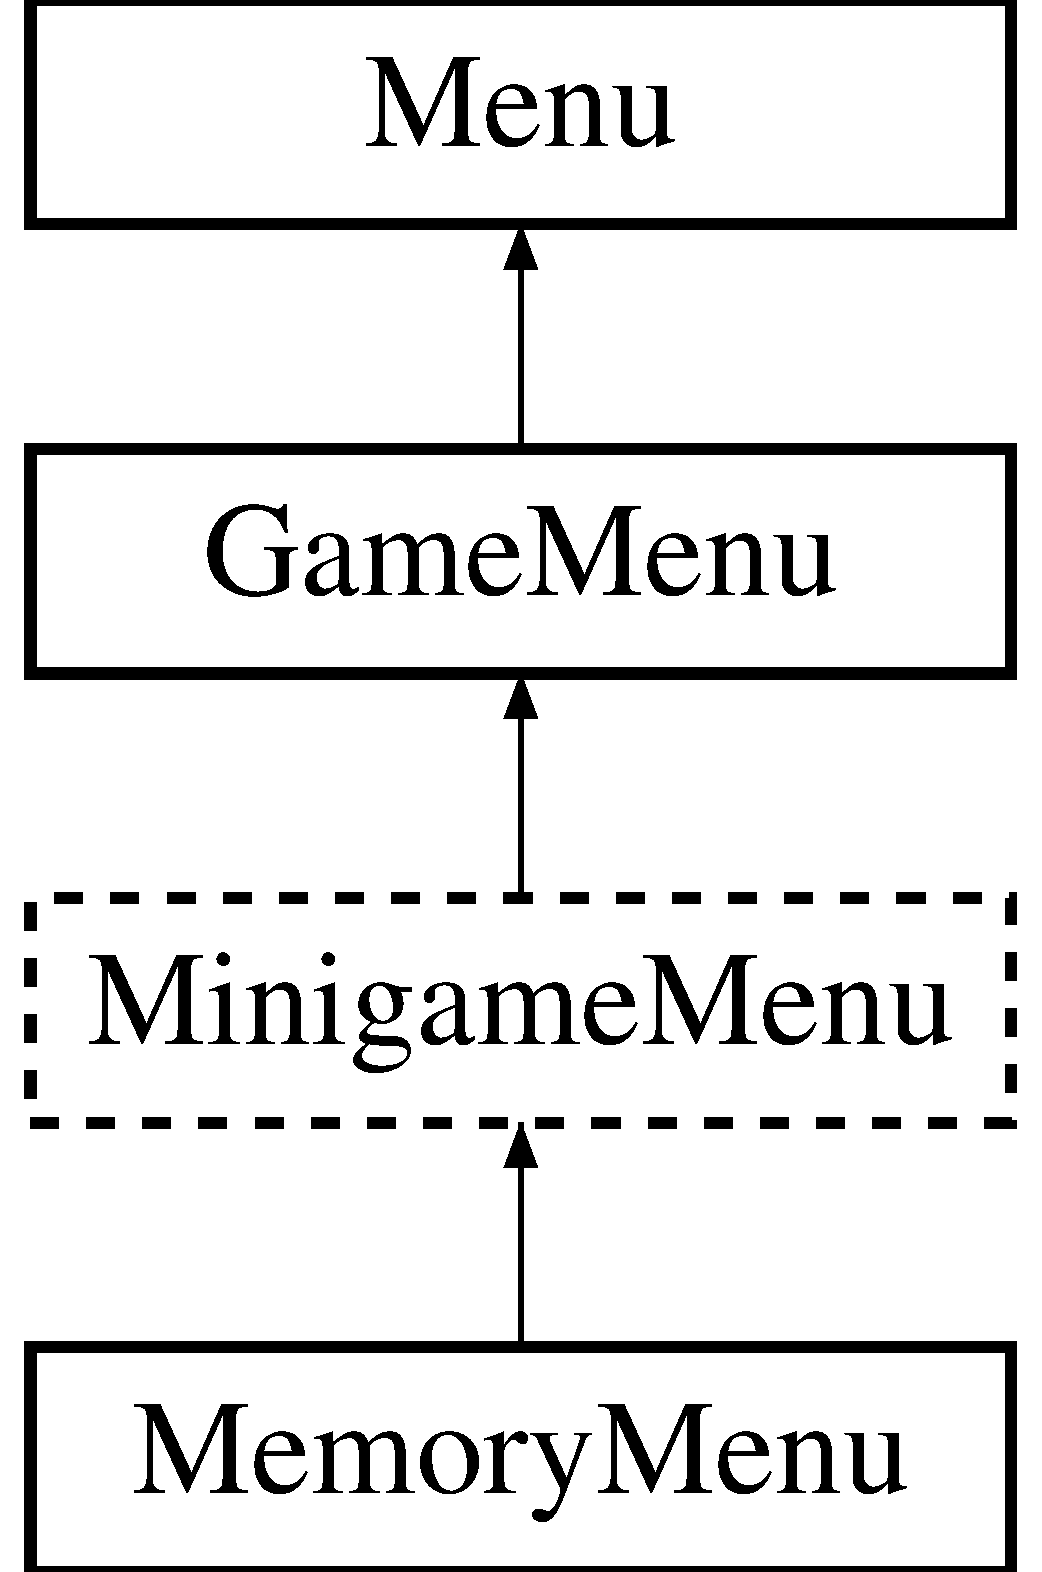
\includegraphics[height=4.000000cm]{classMemoryMenu}
\end{center}
\end{figure}
\subsection*{Classes}
\begin{DoxyCompactItemize}
\item 
struct \hyperlink{structMemoryMenu_1_1Coord}{Coord}
\end{DoxyCompactItemize}
\subsection*{Public Member Functions}
\begin{DoxyCompactItemize}
\item 
\hyperlink{classMemoryMenu_ae86d93eea6621532fba704fed5c9ec33}{Memory\-Menu} ()
\begin{DoxyCompactList}\small\item\em This is the default constructor. \end{DoxyCompactList}\item 
virtual \hyperlink{classMemoryMenu_a4f364ab881bd477e664ef77ceea105fe}{$\sim$\-Memory\-Menu} ()
\begin{DoxyCompactList}\small\item\em This is the virtual destructor. \end{DoxyCompactList}\item 
virtual void \hyperlink{classMemoryMenu_acde088f671d95d13f50b27ac345d2968}{Set\-Options} (int row, int col, int space)
\item 
virtual void \hyperlink{classMemoryMenu_afbe9762ac2e61c6eba82df18aa9aea73}{Handle\-Input} (istream \&is)
\item 
\hyperlink{structMemoryMenu_1_1Coord}{Coord} \hyperlink{classMemoryMenu_afc417793ed520f9382f106d05cf26286}{Get\-Coordinates} () const 
\begin{DoxyCompactList}\small\item\em This function returns the coordinates the player entered. \end{DoxyCompactList}\end{DoxyCompactItemize}
\subsection*{Private Attributes}
\begin{DoxyCompactItemize}
\item 
\hyperlink{structMemoryMenu_1_1Coord}{Coord} \hyperlink{classMemoryMenu_aa29295841088ab4c667a88ae91a0dd45}{coordinates}
\item 
string \hyperlink{classMemoryMenu_af0e3a6658007f4782d181f19d39719f4}{query}
\end{DoxyCompactItemize}
\subsection*{Additional Inherited Members}


\subsection{Detailed Description}
This is the menu class for the Memory match minigame. 

\subsection{Constructor \& Destructor Documentation}
\hypertarget{classMemoryMenu_ae86d93eea6621532fba704fed5c9ec33}{\index{Memory\-Menu@{Memory\-Menu}!Memory\-Menu@{Memory\-Menu}}
\index{Memory\-Menu@{Memory\-Menu}!MemoryMenu@{Memory\-Menu}}
\subsubsection[{Memory\-Menu}]{\setlength{\rightskip}{0pt plus 5cm}Memory\-Menu\-::\-Memory\-Menu (
\begin{DoxyParamCaption}
{}
\end{DoxyParamCaption}
)}}\label{classMemoryMenu_ae86d93eea6621532fba704fed5c9ec33}


This is the default constructor. 

\begin{DoxyDate}{Date}
24/10/2017 
\end{DoxyDate}
\begin{DoxyAuthor}{Author}
Tomas Rigaux
\end{DoxyAuthor}
This is the menu class for the Memory Match minigame. It is a subclass of \hyperlink{classMinigameMenu}{Minigame\-Menu}. \hypertarget{classMemoryMenu_a4f364ab881bd477e664ef77ceea105fe}{\index{Memory\-Menu@{Memory\-Menu}!$\sim$\-Memory\-Menu@{$\sim$\-Memory\-Menu}}
\index{$\sim$\-Memory\-Menu@{$\sim$\-Memory\-Menu}!MemoryMenu@{Memory\-Menu}}
\subsubsection[{$\sim$\-Memory\-Menu}]{\setlength{\rightskip}{0pt plus 5cm}Memory\-Menu\-::$\sim$\-Memory\-Menu (
\begin{DoxyParamCaption}
{}
\end{DoxyParamCaption}
)\hspace{0.3cm}{\ttfamily [virtual]}}}\label{classMemoryMenu_a4f364ab881bd477e664ef77ceea105fe}


This is the virtual destructor. 



\subsection{Member Function Documentation}
\hypertarget{classMemoryMenu_afc417793ed520f9382f106d05cf26286}{\index{Memory\-Menu@{Memory\-Menu}!Get\-Coordinates@{Get\-Coordinates}}
\index{Get\-Coordinates@{Get\-Coordinates}!MemoryMenu@{Memory\-Menu}}
\subsubsection[{Get\-Coordinates}]{\setlength{\rightskip}{0pt plus 5cm}{\bf Memory\-Menu\-::\-Coord} Memory\-Menu\-::\-Get\-Coordinates (
\begin{DoxyParamCaption}
{}
\end{DoxyParamCaption}
) const}}\label{classMemoryMenu_afc417793ed520f9382f106d05cf26286}


This function returns the coordinates the player entered. 

\hypertarget{classMemoryMenu_afbe9762ac2e61c6eba82df18aa9aea73}{\index{Memory\-Menu@{Memory\-Menu}!Handle\-Input@{Handle\-Input}}
\index{Handle\-Input@{Handle\-Input}!MemoryMenu@{Memory\-Menu}}
\subsubsection[{Handle\-Input}]{\setlength{\rightskip}{0pt plus 5cm}void Memory\-Menu\-::\-Handle\-Input (
\begin{DoxyParamCaption}
\item[{istream \&}]{is}
\end{DoxyParamCaption}
)\hspace{0.3cm}{\ttfamily [virtual]}}}\label{classMemoryMenu_afbe9762ac2e61c6eba82df18aa9aea73}
This function handles the input for the menu options. 
\begin{DoxyParams}[1]{Parameters}
\mbox{\tt in,out}  & {\em is} & The in-\/stream operator to read the input. \\
\hline
\end{DoxyParams}


Implements \hyperlink{classMinigameMenu_a3f854c4eefb0f3110cd085b3cfe56460}{Minigame\-Menu}.

\hypertarget{classMemoryMenu_acde088f671d95d13f50b27ac345d2968}{\index{Memory\-Menu@{Memory\-Menu}!Set\-Options@{Set\-Options}}
\index{Set\-Options@{Set\-Options}!MemoryMenu@{Memory\-Menu}}
\subsubsection[{Set\-Options}]{\setlength{\rightskip}{0pt plus 5cm}void Memory\-Menu\-::\-Set\-Options (
\begin{DoxyParamCaption}
\item[{int}]{row, }
\item[{int}]{col, }
\item[{int}]{space}
\end{DoxyParamCaption}
)\hspace{0.3cm}{\ttfamily [virtual]}}}\label{classMemoryMenu_acde088f671d95d13f50b27ac345d2968}
This function sets the specific options for the \hyperlink{classMenu}{Menu} type. 
\begin{DoxyParams}[1]{Parameters}
\mbox{\tt in}  & {\em Options\-List} & A map of all the options for the current menu. Each option has a unique key to make input easier. \\
\hline
\mbox{\tt in}  & {\em type} & This denotes the type of menu to display. \\
\hline
\end{DoxyParams}


Implements \hyperlink{classMinigameMenu_abde3ae319bf1660a8626c6f765e054a8}{Minigame\-Menu}.



\subsection{Member Data Documentation}
\hypertarget{classMemoryMenu_aa29295841088ab4c667a88ae91a0dd45}{\index{Memory\-Menu@{Memory\-Menu}!coordinates@{coordinates}}
\index{coordinates@{coordinates}!MemoryMenu@{Memory\-Menu}}
\subsubsection[{coordinates}]{\setlength{\rightskip}{0pt plus 5cm}{\bf Coord} Memory\-Menu\-::coordinates\hspace{0.3cm}{\ttfamily [private]}}}\label{classMemoryMenu_aa29295841088ab4c667a88ae91a0dd45}
\hypertarget{classMemoryMenu_af0e3a6658007f4782d181f19d39719f4}{\index{Memory\-Menu@{Memory\-Menu}!query@{query}}
\index{query@{query}!MemoryMenu@{Memory\-Menu}}
\subsubsection[{query}]{\setlength{\rightskip}{0pt plus 5cm}string Memory\-Menu\-::query\hspace{0.3cm}{\ttfamily [private]}}}\label{classMemoryMenu_af0e3a6658007f4782d181f19d39719f4}


The documentation for this class was generated from the following files\-:\begin{DoxyCompactItemize}
\item 
/home/rigt2720/\-Kodika/\-Menu/\hyperlink{MemoryMenu_8h}{Memory\-Menu.\-h}\item 
/home/rigt2720/\-Kodika/\-Menu/\hyperlink{MemoryMenu_8cpp}{Memory\-Menu.\-cpp}\end{DoxyCompactItemize}

\hypertarget{classMenu}{\section{Menu Class Reference}
\label{classMenu}\index{Menu@{Menu}}
}


This is the base class for all menus for the main game.  




{\ttfamily \#include $<$Menu.\-h$>$}

Inheritance diagram for Menu\-:\begin{figure}[H]
\begin{center}
\leavevmode
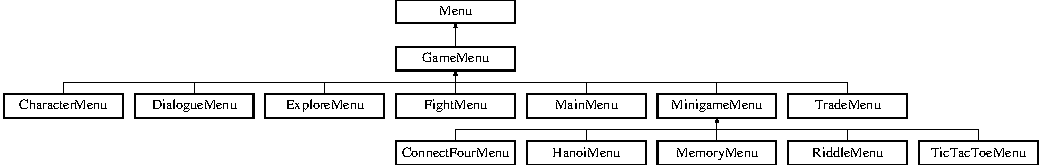
\includegraphics[height=4.000000cm]{classMenu}
\end{center}
\end{figure}
\subsection*{Public Member Functions}
\begin{DoxyCompactItemize}
\item 
\hyperlink{classMenu_a5a60e837b160444bee4525c06fd4c51e}{Menu} (int height=10, int width=100)
\item 
\hypertarget{classMenu_a831387f51358cfb88cd018e1777bc980}{virtual \hyperlink{classMenu_a831387f51358cfb88cd018e1777bc980}{$\sim$\-Menu} ()}\label{classMenu_a831387f51358cfb88cd018e1777bc980}

\begin{DoxyCompactList}\small\item\em This is the destructor for the class. It is virtual. \end{DoxyCompactList}\item 
\hypertarget{classMenu_a8451a530cd2b53f456658f8741ae45bb}{virtual void {\bfseries Set\-Options} (map$<$ int, string $>$ Options\-List, string type=\char`\"{}generic\char`\"{})}\label{classMenu_a8451a530cd2b53f456658f8741ae45bb}

\item 
virtual void \hyperlink{classMenu_a81bb84f921911944e4060d1c5a1b2507}{Handle\-Option\-Input} (istream \&is)
\item 
\hypertarget{classMenu_a4665a914fe24a8b11d8d6c95792184b3}{virtual void \hyperlink{classMenu_a4665a914fe24a8b11d8d6c95792184b3}{Output\-Menu} ()}\label{classMenu_a4665a914fe24a8b11d8d6c95792184b3}

\begin{DoxyCompactList}\small\item\em Display the multi-\/dimensional array. \end{DoxyCompactList}\end{DoxyCompactItemize}
\subsection*{Protected Member Functions}
\begin{DoxyCompactItemize}
\item 
void \hyperlink{classMenu_a09adbf38cefb171f8f06536c881d3944}{set} (int x, int y, char ch)
\end{DoxyCompactItemize}


\subsection{Detailed Description}
This is the base class for all menus for the main game. 

\subsection{Constructor \& Destructor Documentation}
\hypertarget{classMenu_a5a60e837b160444bee4525c06fd4c51e}{\index{Menu@{Menu}!Menu@{Menu}}
\index{Menu@{Menu}!Menu@{Menu}}
\subsubsection[{Menu}]{\setlength{\rightskip}{0pt plus 5cm}Menu\-::\-Menu (
\begin{DoxyParamCaption}
\item[{int}]{height = {\ttfamily 10}, }
\item[{int}]{width = {\ttfamily 100}}
\end{DoxyParamCaption}
)}}\label{classMenu_a5a60e837b160444bee4525c06fd4c51e}
Sets the various options for the menu, mapping them to unique keys to make handling easier. 
\begin{DoxyParams}[1]{Parameters}
\mbox{\tt in}  & {\em Options\-List} & A map of all the options for the current menu. Each option has a unique key to make input easier. \\
\hline
\mbox{\tt in}  & {\em type} & This denotes the type of menu to display. This is the constructor. It initializes a multi-\/dimensional array to dimensions height$\ast$width. \\
\hline
\mbox{\tt in}  & {\em height} & This is the height of the menu. \\
\hline
\mbox{\tt in}  & {\em width} & This is the width of the menu. \\
\hline
\end{DoxyParams}


\subsection{Member Function Documentation}
\hypertarget{classMenu_a81bb84f921911944e4060d1c5a1b2507}{\index{Menu@{Menu}!Handle\-Option\-Input@{Handle\-Option\-Input}}
\index{Handle\-Option\-Input@{Handle\-Option\-Input}!Menu@{Menu}}
\subsubsection[{Handle\-Option\-Input}]{\setlength{\rightskip}{0pt plus 5cm}void Menu\-::\-Handle\-Option\-Input (
\begin{DoxyParamCaption}
\item[{istream \&}]{is}
\end{DoxyParamCaption}
)\hspace{0.3cm}{\ttfamily [virtual]}}}\label{classMenu_a81bb84f921911944e4060d1c5a1b2507}
Handles the user input, and runs an option from the menu. 
\begin{DoxyParams}[1]{Parameters}
\mbox{\tt in,out}  & {\em is} & The in-\/stream operator to read the input. \\
\hline
\end{DoxyParams}
\hypertarget{classMenu_a09adbf38cefb171f8f06536c881d3944}{\index{Menu@{Menu}!set@{set}}
\index{set@{set}!Menu@{Menu}}
\subsubsection[{set}]{\setlength{\rightskip}{0pt plus 5cm}void Menu\-::set (
\begin{DoxyParamCaption}
\item[{int}]{x, }
\item[{int}]{y, }
\item[{char}]{ch}
\end{DoxyParamCaption}
)\hspace{0.3cm}{\ttfamily [protected]}}}\label{classMenu_a09adbf38cefb171f8f06536c881d3944}
Sets the character of a specific location in the array to a give character. 
\begin{DoxyParams}[1]{Parameters}
\mbox{\tt in}  & {\em x} & This is the x-\/coordinate of the multi-\/dimensional array. (A\mbox{[}x,y\mbox{]}) \\
\hline
\mbox{\tt in}  & {\em y} & This is the y-\/coordinate of the multi-\/dimensional array. (A\mbox{[}x,y\mbox{]}) \\
\hline
\mbox{\tt in}  & {\em ch} & This is the character to be set at the coordinates (x,y) in the multi-\/dimensional array. \\
\hline
\end{DoxyParams}


The documentation for this class was generated from the following files\-:\begin{DoxyCompactItemize}
\item 
Menu/Menu.\-h\item 
Menu/Menu.\-cpp\item 
Puzzles/Menu.\-cpp\end{DoxyCompactItemize}

\hypertarget{classMenuTest}{\section{Menu\-Test Class Reference}
\label{classMenuTest}\index{Menu\-Test@{Menu\-Test}}
}


Test class for the \hyperlink{classMenu}{Menu} class.  




{\ttfamily \#include $<$Menu\-Test.\-h$>$}

Inheritance diagram for Menu\-Test\-:\begin{figure}[H]
\begin{center}
\leavevmode
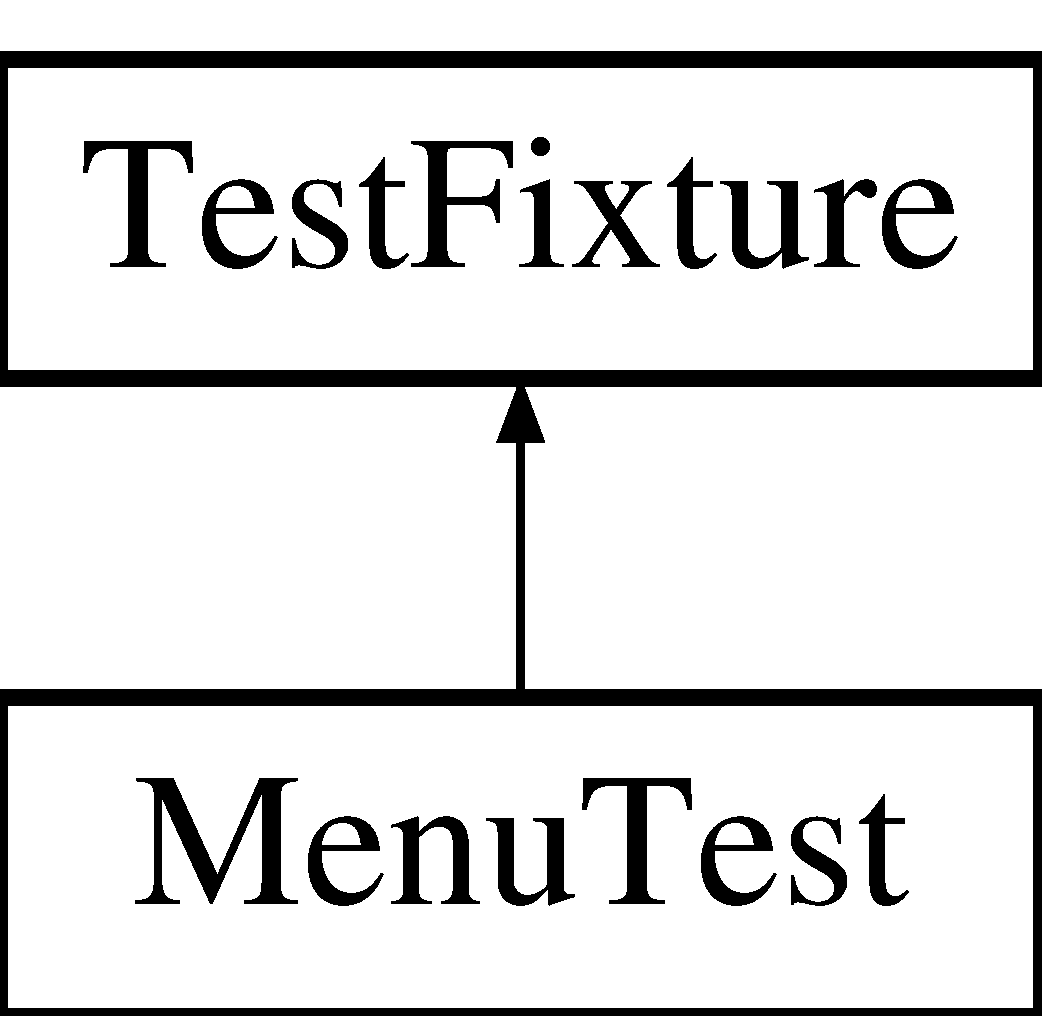
\includegraphics[height=2.000000cm]{classMenuTest}
\end{center}
\end{figure}
\subsection*{Public Member Functions}
\begin{DoxyCompactItemize}
\item 
void \hyperlink{classMenuTest_afe356a4dfec90fec48cdfb5a31292dda}{Set\-Up} ()
\begin{DoxyCompactList}\small\item\em Sets up the test variables for testing. \end{DoxyCompactList}\item 
\hypertarget{classMenuTest_abd39213e0c7d442794d552460d920865}{void \hyperlink{classMenuTest_abd39213e0c7d442794d552460d920865}{Tear\-Down} ()}\label{classMenuTest_abd39213e0c7d442794d552460d920865}

\begin{DoxyCompactList}\small\item\em Deletes any pointers to prevent memory leak. \end{DoxyCompactList}\item 
\hypertarget{classMenuTest_a8937223971935c31487f46a00d294e97}{void \hyperlink{classMenuTest_a8937223971935c31487f46a00d294e97}{Test\-Constructors} ()}\label{classMenuTest_a8937223971935c31487f46a00d294e97}

\begin{DoxyCompactList}\small\item\em Tests that the constructor is wokring in several varieties of construction. \end{DoxyCompactList}\item 
\hypertarget{classMenuTest_ab0a87d1e4ee856ccf3af3cc6663845c4}{void \hyperlink{classMenuTest_ab0a87d1e4ee856ccf3af3cc6663845c4}{Test\-Setting} ()}\label{classMenuTest_ab0a87d1e4ee856ccf3af3cc6663845c4}

\begin{DoxyCompactList}\small\item\em Tests the setting of options. \end{DoxyCompactList}\item 
\hypertarget{classMenuTest_af74ddfe672fb68438b3e966c3736a763}{void \hyperlink{classMenuTest_af74ddfe672fb68438b3e966c3736a763}{Test\-Building} ()}\label{classMenuTest_af74ddfe672fb68438b3e966c3736a763}

\begin{DoxyCompactList}\small\item\em Tests that menu builds correctly. \end{DoxyCompactList}\end{DoxyCompactItemize}


\subsection{Detailed Description}
Test class for the \hyperlink{classMenu}{Menu} class. 

\begin{DoxyAuthor}{Author}
Tomas Rigaux 
\end{DoxyAuthor}
\begin{DoxyDate}{Date}
8/11/2017
\end{DoxyDate}
This is the testing class for \hyperlink{classMenu}{Menu}. 

\subsection{Member Function Documentation}
\hypertarget{classMenuTest_afe356a4dfec90fec48cdfb5a31292dda}{\index{Menu\-Test@{Menu\-Test}!Set\-Up@{Set\-Up}}
\index{Set\-Up@{Set\-Up}!MenuTest@{Menu\-Test}}
\subsubsection[{Set\-Up}]{\setlength{\rightskip}{0pt plus 5cm}void Menu\-Test\-::\-Set\-Up (
\begin{DoxyParamCaption}
{}
\end{DoxyParamCaption}
)}}\label{classMenuTest_afe356a4dfec90fec48cdfb5a31292dda}


Sets up the test variables for testing. 

\begin{DoxyAuthor}{Author}
Tomas Rigaux 
\end{DoxyAuthor}
\begin{DoxyDate}{Date}
8/11/2017
\end{DoxyDate}
This is the testing class for \hyperlink{classMenu}{Menu}. 

The documentation for this class was generated from the following files\-:\begin{DoxyCompactItemize}
\item 
Menu/Menu\-Test.\-h\item 
Menu/Menu\-Test.\-cpp\end{DoxyCompactItemize}

\hypertarget{classMinigameMenu}{\section{Minigame\-Menu Class Reference}
\label{classMinigameMenu}\index{Minigame\-Menu@{Minigame\-Menu}}
}


An abstract class, this is the base class for the all the in-\/game puzzle/minigame menu classes.  




{\ttfamily \#include $<$Minigame\-Menu.\-h$>$}

Inheritance diagram for Minigame\-Menu\-:\begin{figure}[H]
\begin{center}
\leavevmode
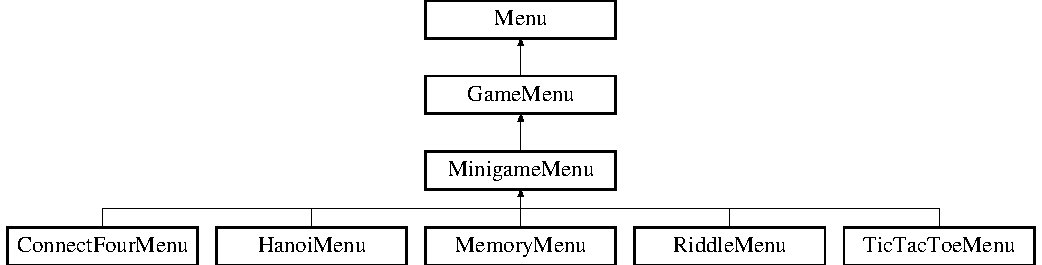
\includegraphics[height=3.555556cm]{classMinigameMenu}
\end{center}
\end{figure}
\subsection*{Public Member Functions}
\begin{DoxyCompactItemize}
\item 
\hyperlink{classMinigameMenu_a90d42578d68f68c3b26c414f90f2d950}{Minigame\-Menu} ()
\begin{DoxyCompactList}\small\item\em This is the default constructor. \end{DoxyCompactList}\item 
virtual \hyperlink{classMinigameMenu_a6b8621ca44319d6b2759766bdca9cbf9}{$\sim$\-Minigame\-Menu} ()
\begin{DoxyCompactList}\small\item\em This is the virtual destructor. \end{DoxyCompactList}\item 
virtual void \hyperlink{classMinigameMenu_abde3ae319bf1660a8626c6f765e054a8}{Set\-Options} (int row, int col, int space)=0
\item 
virtual void \hyperlink{classMinigameMenu_a3f854c4eefb0f3110cd085b3cfe56460}{Handle\-Input} (istream \&is)=0
\item 
void \hyperlink{classMinigameMenu_a875e8a60a910f28e245c998772d043e4}{Set\-Query} (string q)
\begin{DoxyCompactList}\small\item\em Allows the query to be set. \end{DoxyCompactList}\end{DoxyCompactItemize}
\subsection*{Protected Attributes}
\begin{DoxyCompactItemize}
\item 
string \hyperlink{classMinigameMenu_a5c36c7797c89ff8d0e6646800b0de38a}{query}
\begin{DoxyCompactList}\small\item\em Sets the query of the game. \end{DoxyCompactList}\end{DoxyCompactItemize}
\subsection*{Additional Inherited Members}


\subsection{Detailed Description}
An abstract class, this is the base class for the all the in-\/game puzzle/minigame menu classes. 

\subsection{Constructor \& Destructor Documentation}
\hypertarget{classMinigameMenu_a90d42578d68f68c3b26c414f90f2d950}{\index{Minigame\-Menu@{Minigame\-Menu}!Minigame\-Menu@{Minigame\-Menu}}
\index{Minigame\-Menu@{Minigame\-Menu}!MinigameMenu@{Minigame\-Menu}}
\subsubsection[{Minigame\-Menu}]{\setlength{\rightskip}{0pt plus 5cm}Minigame\-Menu\-::\-Minigame\-Menu (
\begin{DoxyParamCaption}
{}
\end{DoxyParamCaption}
)\hspace{0.3cm}{\ttfamily [inline]}}}\label{classMinigameMenu_a90d42578d68f68c3b26c414f90f2d950}


This is the default constructor. 

\hypertarget{classMinigameMenu_a6b8621ca44319d6b2759766bdca9cbf9}{\index{Minigame\-Menu@{Minigame\-Menu}!$\sim$\-Minigame\-Menu@{$\sim$\-Minigame\-Menu}}
\index{$\sim$\-Minigame\-Menu@{$\sim$\-Minigame\-Menu}!MinigameMenu@{Minigame\-Menu}}
\subsubsection[{$\sim$\-Minigame\-Menu}]{\setlength{\rightskip}{0pt plus 5cm}virtual Minigame\-Menu\-::$\sim$\-Minigame\-Menu (
\begin{DoxyParamCaption}
{}
\end{DoxyParamCaption}
)\hspace{0.3cm}{\ttfamily [inline]}, {\ttfamily [virtual]}}}\label{classMinigameMenu_a6b8621ca44319d6b2759766bdca9cbf9}


This is the virtual destructor. 



\subsection{Member Function Documentation}
\hypertarget{classMinigameMenu_a3f854c4eefb0f3110cd085b3cfe56460}{\index{Minigame\-Menu@{Minigame\-Menu}!Handle\-Input@{Handle\-Input}}
\index{Handle\-Input@{Handle\-Input}!MinigameMenu@{Minigame\-Menu}}
\subsubsection[{Handle\-Input}]{\setlength{\rightskip}{0pt plus 5cm}virtual void Minigame\-Menu\-::\-Handle\-Input (
\begin{DoxyParamCaption}
\item[{istream \&}]{is}
\end{DoxyParamCaption}
)\hspace{0.3cm}{\ttfamily [pure virtual]}}}\label{classMinigameMenu_a3f854c4eefb0f3110cd085b3cfe56460}
This function handles the input for the menu options. 
\begin{DoxyParams}[1]{Parameters}
\mbox{\tt in,out}  & {\em is} & The in-\/stream operator to read the input. \\
\hline
\end{DoxyParams}


Implements \hyperlink{classGameMenu_a02ba09feedece5773f44ba865ccffb42}{Game\-Menu}.



Implemented in \hyperlink{classMemoryMenu_afbe9762ac2e61c6eba82df18aa9aea73}{Memory\-Menu}, \hyperlink{classTicTacToeMenu_a11191814019309260bb4270c03891e5e}{Tic\-Tac\-Toe\-Menu}, \hyperlink{classConnectFourMenu_a2af0c62dd776dd0e3d8c212f71eb3219}{Connect\-Four\-Menu}, \hyperlink{classHanoiMenu_a8f85bae3166bf122c5800aab41c87d54}{Hanoi\-Menu}, and \hyperlink{classRiddleMenu_aef67f984c1aad0b8240e03b43ccbe615}{Riddle\-Menu}.

\hypertarget{classMinigameMenu_abde3ae319bf1660a8626c6f765e054a8}{\index{Minigame\-Menu@{Minigame\-Menu}!Set\-Options@{Set\-Options}}
\index{Set\-Options@{Set\-Options}!MinigameMenu@{Minigame\-Menu}}
\subsubsection[{Set\-Options}]{\setlength{\rightskip}{0pt plus 5cm}virtual void Minigame\-Menu\-::\-Set\-Options (
\begin{DoxyParamCaption}
\item[{int}]{row, }
\item[{int}]{col, }
\item[{int}]{space}
\end{DoxyParamCaption}
)\hspace{0.3cm}{\ttfamily [pure virtual]}}}\label{classMinigameMenu_abde3ae319bf1660a8626c6f765e054a8}
This function sets the specific options for the minigame. 
\begin{DoxyParams}[1]{Parameters}
\mbox{\tt in}  & {\em row} & Determines which row the options will start being set at. \\
\hline
\mbox{\tt in}  & {\em col} & Determines which column the options will start from. \\
\hline
\mbox{\tt in}  & {\em How} & mush space inbetween rows. \\
\hline
\end{DoxyParams}


Implements \hyperlink{classGameMenu_ac32ff465c5a4f30979e8851fa21cb230}{Game\-Menu}.



Implemented in \hyperlink{classMemoryMenu_acde088f671d95d13f50b27ac345d2968}{Memory\-Menu}, \hyperlink{classTicTacToeMenu_ab736aba3ecb23a6b28cde04729556088}{Tic\-Tac\-Toe\-Menu}, \hyperlink{classConnectFourMenu_a6a826d0810795584cfb4b601d5cd5df2}{Connect\-Four\-Menu}, \hyperlink{classHanoiMenu_a0280d0e443642407fda5903346be1a39}{Hanoi\-Menu}, and \hyperlink{classRiddleMenu_a2d103283c58744ffa0e77e62a24e7ccb}{Riddle\-Menu}.

\hypertarget{classMinigameMenu_a875e8a60a910f28e245c998772d043e4}{\index{Minigame\-Menu@{Minigame\-Menu}!Set\-Query@{Set\-Query}}
\index{Set\-Query@{Set\-Query}!MinigameMenu@{Minigame\-Menu}}
\subsubsection[{Set\-Query}]{\setlength{\rightskip}{0pt plus 5cm}void Minigame\-Menu\-::\-Set\-Query (
\begin{DoxyParamCaption}
\item[{string}]{q}
\end{DoxyParamCaption}
)\hspace{0.3cm}{\ttfamily [inline]}}}\label{classMinigameMenu_a875e8a60a910f28e245c998772d043e4}


Allows the query to be set. 



\subsection{Member Data Documentation}
\hypertarget{classMinigameMenu_a5c36c7797c89ff8d0e6646800b0de38a}{\index{Minigame\-Menu@{Minigame\-Menu}!query@{query}}
\index{query@{query}!MinigameMenu@{Minigame\-Menu}}
\subsubsection[{query}]{\setlength{\rightskip}{0pt plus 5cm}string Minigame\-Menu\-::query\hspace{0.3cm}{\ttfamily [protected]}}}\label{classMinigameMenu_a5c36c7797c89ff8d0e6646800b0de38a}


Sets the query of the game. 



The documentation for this class was generated from the following file\-:\begin{DoxyCompactItemize}
\item 
/home/rigt2720/\-Kodika/\-Menu/\hyperlink{MinigameMenu_8h}{Minigame\-Menu.\-h}\end{DoxyCompactItemize}

\hypertarget{classNpc}{\section{Npc Class Reference}
\label{classNpc}\index{Npc@{Npc}}
}


Derived class from \hyperlink{classCharacter}{Character} which provides \hyperlink{classNpc}{Npc} attributes.  




{\ttfamily \#include $<$Npc.\-h$>$}

Inheritance diagram for Npc\-:\begin{figure}[H]
\begin{center}
\leavevmode
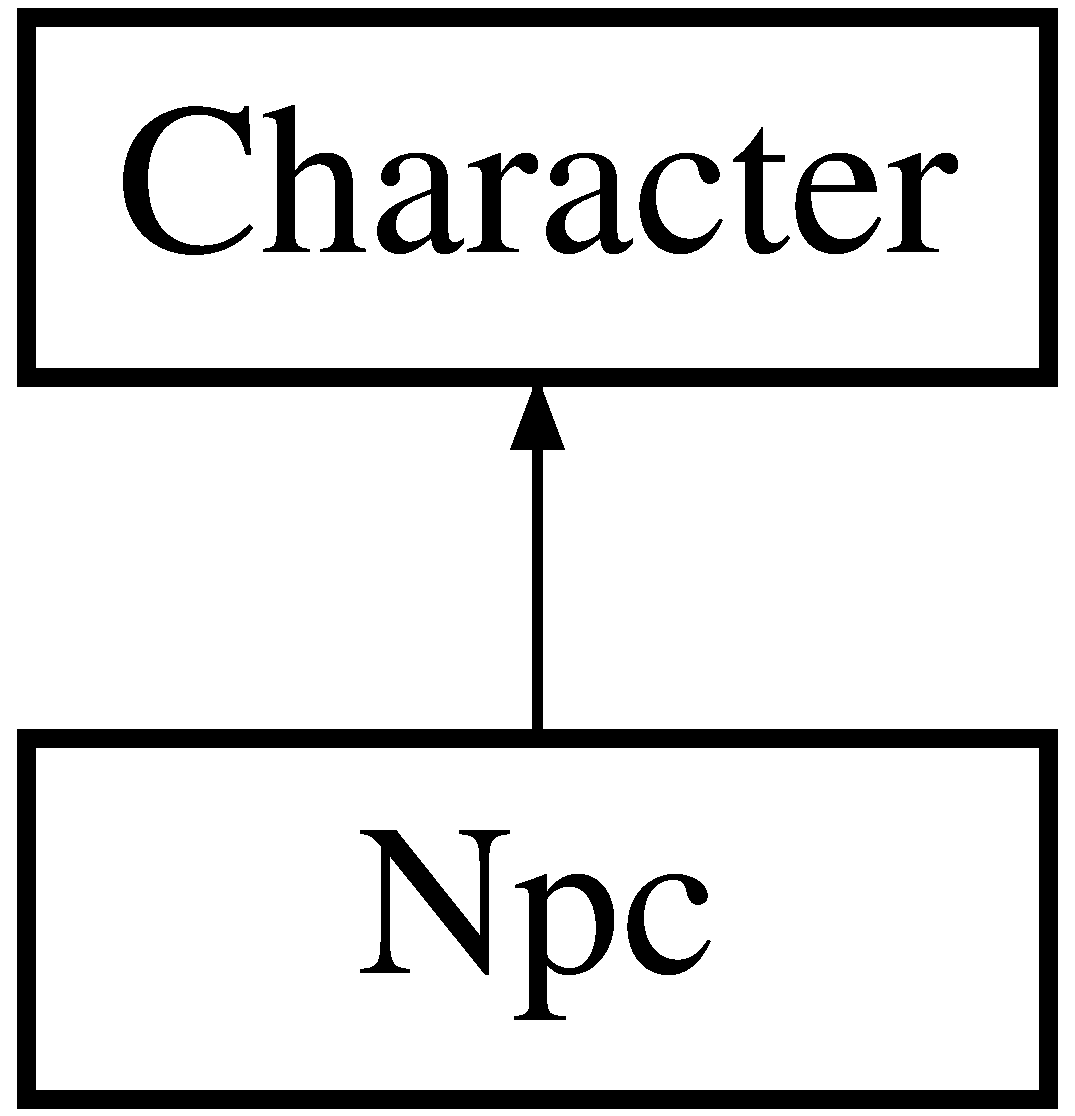
\includegraphics[height=2.000000cm]{classNpc}
\end{center}
\end{figure}
\subsection*{Public Member Functions}
\begin{DoxyCompactItemize}
\item 
\hyperlink{classNpc_ad8de4e512338f57a56f490c60293118b}{Npc} (int s=0, int g=0, int h=0, \hyperlink{classImportImg}{Import\-Img} \hyperlink{classCharacter_a3a0a90b2a43858b259912f659b8e0eea}{img}=\hyperlink{classImportImg}{Import\-Img}(\char`\"{}../D\-D\-\_\-\-Art/\hyperlink{classPlayer}{Player}/D\-D\-\_\-\-N\-P\-C\-Enemy.\-txt\char`\"{}))
\item 
\hyperlink{classNpc_a2249c5155af3d692e51ff610064e81fe}{$\sim$\-Npc} ()
\begin{DoxyCompactList}\small\item\em Deconstructor. \end{DoxyCompactList}\end{DoxyCompactItemize}
\subsection*{Additional Inherited Members}


\subsection{Detailed Description}
Derived class from \hyperlink{classCharacter}{Character} which provides \hyperlink{classNpc}{Npc} attributes. 

\subsection{Constructor \& Destructor Documentation}
\hypertarget{classNpc_ad8de4e512338f57a56f490c60293118b}{\index{Npc@{Npc}!Npc@{Npc}}
\index{Npc@{Npc}!Npc@{Npc}}
\subsubsection[{Npc}]{\setlength{\rightskip}{0pt plus 5cm}Npc\-::\-Npc (
\begin{DoxyParamCaption}
\item[{int}]{s = {\ttfamily 0}, }
\item[{int}]{g = {\ttfamily 0}, }
\item[{int}]{h = {\ttfamily 0}, }
\item[{{\bf Import\-Img}}]{img = {\ttfamily {\bf Import\-Img}(\char`\"{}../DD\-\_\-Art/{\bf Player}/DD\-\_\-NPCEnemy.txt\char`\"{})}}
\end{DoxyParamCaption}
)}}\label{classNpc_ad8de4e512338f57a56f490c60293118b}
\hyperlink{classNpc}{Npc} constructor 
\begin{DoxyParams}[1]{Parameters}
\mbox{\tt in}  & {\em h,the} & health of the created \hyperlink{classNpc}{Npc} \\
\hline
\end{DoxyParams}
\hypertarget{classNpc_a2249c5155af3d692e51ff610064e81fe}{\index{Npc@{Npc}!$\sim$\-Npc@{$\sim$\-Npc}}
\index{$\sim$\-Npc@{$\sim$\-Npc}!Npc@{Npc}}
\subsubsection[{$\sim$\-Npc}]{\setlength{\rightskip}{0pt plus 5cm}Npc\-::$\sim$\-Npc (
\begin{DoxyParamCaption}
{}
\end{DoxyParamCaption}
)}}\label{classNpc_a2249c5155af3d692e51ff610064e81fe}


Deconstructor. 



The documentation for this class was generated from the following files\-:\begin{DoxyCompactItemize}
\item 
/home/rigt2720/\-Kodika/\-Character/\hyperlink{Npc_8h}{Npc.\-h}\item 
/home/rigt2720/\-Kodika/\-Character/\hyperlink{Npc_8cpp}{Npc.\-cpp}\end{DoxyCompactItemize}

\hypertarget{classPlayer}{\section{Player Class Reference}
\label{classPlayer}\index{Player@{Player}}
}


Derived class from \hyperlink{classCharacter}{Character} which provides \hyperlink{classPlayer}{Player} attributes.  




{\ttfamily \#include $<$Player.\-h$>$}

\subsection*{Public Member Functions}
\begin{DoxyCompactItemize}
\item 
\hyperlink{classPlayer_a3f78353312cc3cf41905fdc3accafb6c}{Player} (int s=0, int k=0, string n=\char`\"{} \char`\"{}, string r=\char`\"{} \char`\"{})
\item 
\hyperlink{classPlayer_a749d2c00e1fe0f5c2746f7505a58c062}{$\sim$\-Player} ()
\begin{DoxyCompactList}\small\item\em \hyperlink{classPlayer}{Player} deconstructor. \end{DoxyCompactList}\item 
void \hyperlink{classPlayer_a5bca1aa08cadb57984c488498a2e0e38}{Change\-Stamina} (int \&s, int s\-Mod)
\item 
void \hyperlink{classPlayer_a325d080bde1038593f942b17a5dd6ae2}{Change\-Keys} (int \&\hyperlink{classPlayer_ac46baa685ca2a266178f03b9e9877e65}{keys}, int key\-Mod)
\item 
bool \hyperlink{classPlayer_af839bdc1524d571568ea31a34f44f3ab}{Use\-Key} (int \&\hyperlink{classPlayer_ac46baa685ca2a266178f03b9e9877e65}{keys})
\end{DoxyCompactItemize}
\subsection*{Private Attributes}
\begin{DoxyCompactItemize}
\item 
string \hyperlink{classPlayer_acf0355128a99ee20ad9931b760fb2de1}{name}
\begin{DoxyCompactList}\small\item\em Name of the player. \end{DoxyCompactList}\item 
string \hyperlink{classPlayer_a5130cb6c4233cd7ad1212af0d1790e58}{race}
\begin{DoxyCompactList}\small\item\em Race of the player. \end{DoxyCompactList}\item 
int \hyperlink{classPlayer_a3642fc1d242a769a2ea76dc0b1662a20}{stamina}
\begin{DoxyCompactList}\small\item\em Players stamina. \end{DoxyCompactList}\item 
int \hyperlink{classPlayer_ac46baa685ca2a266178f03b9e9877e65}{keys}
\begin{DoxyCompactList}\small\item\em Amoutn of keys player has. \end{DoxyCompactList}\end{DoxyCompactItemize}


\subsection{Detailed Description}
Derived class from \hyperlink{classCharacter}{Character} which provides \hyperlink{classPlayer}{Player} attributes. 

\subsection{Constructor \& Destructor Documentation}
\hypertarget{classPlayer_a3f78353312cc3cf41905fdc3accafb6c}{\index{Player@{Player}!Player@{Player}}
\index{Player@{Player}!Player@{Player}}
\subsubsection[{Player}]{\setlength{\rightskip}{0pt plus 5cm}Player\-::\-Player (
\begin{DoxyParamCaption}
\item[{int}]{s = {\ttfamily 0}, }
\item[{int}]{k = {\ttfamily 0}, }
\item[{string}]{n = {\ttfamily \char`\"{}~\char`\"{}}, }
\item[{string}]{r = {\ttfamily \char`\"{}~\char`\"{}}}
\end{DoxyParamCaption}
)}}\label{classPlayer_a3f78353312cc3cf41905fdc3accafb6c}
\hyperlink{classPlayer}{Player} constructor 
\begin{DoxyParams}[1]{Parameters}
\mbox{\tt in}  & {\em s,players} & stamina \\
\hline
\mbox{\tt in}  & {\em k,players} & keys \\
\hline
\mbox{\tt in}  & {\em n,players} & name \\
\hline
\mbox{\tt in}  & {\em r,players} & race \\
\hline
\end{DoxyParams}
\hypertarget{classPlayer_a749d2c00e1fe0f5c2746f7505a58c062}{\index{Player@{Player}!$\sim$\-Player@{$\sim$\-Player}}
\index{$\sim$\-Player@{$\sim$\-Player}!Player@{Player}}
\subsubsection[{$\sim$\-Player}]{\setlength{\rightskip}{0pt plus 5cm}Player\-::$\sim$\-Player (
\begin{DoxyParamCaption}
{}
\end{DoxyParamCaption}
)}}\label{classPlayer_a749d2c00e1fe0f5c2746f7505a58c062}


\hyperlink{classPlayer}{Player} deconstructor. 



\subsection{Member Function Documentation}
\hypertarget{classPlayer_a325d080bde1038593f942b17a5dd6ae2}{\index{Player@{Player}!Change\-Keys@{Change\-Keys}}
\index{Change\-Keys@{Change\-Keys}!Player@{Player}}
\subsubsection[{Change\-Keys}]{\setlength{\rightskip}{0pt plus 5cm}void Player\-::\-Change\-Keys (
\begin{DoxyParamCaption}
\item[{int \&}]{keys, }
\item[{int}]{key\-Mod}
\end{DoxyParamCaption}
)}}\label{classPlayer_a325d080bde1038593f942b17a5dd6ae2}
Amount of keys the player has 
\begin{DoxyParams}[1]{Parameters}
 & {\em in\&\mbox{]}} & keys, current amount of keys the player has \\
\hline
\mbox{\tt in}  & {\em key\-Mod,how} & the current amount of keys will be modified \\
\hline
\end{DoxyParams}
\hypertarget{classPlayer_a5bca1aa08cadb57984c488498a2e0e38}{\index{Player@{Player}!Change\-Stamina@{Change\-Stamina}}
\index{Change\-Stamina@{Change\-Stamina}!Player@{Player}}
\subsubsection[{Change\-Stamina}]{\setlength{\rightskip}{0pt plus 5cm}void Player\-::\-Change\-Stamina (
\begin{DoxyParamCaption}
\item[{int \&}]{s, }
\item[{int}]{s\-Mod}
\end{DoxyParamCaption}
)}}\label{classPlayer_a5bca1aa08cadb57984c488498a2e0e38}
Changes players stamina 
\begin{DoxyParams}[1]{Parameters}
 & {\em in\&\mbox{]}} & s, players current stamina \\
\hline
\mbox{\tt in}  & {\em s\-Mod,how} & the curent stamina will be modified \\
\hline
\end{DoxyParams}
\hypertarget{classPlayer_af839bdc1524d571568ea31a34f44f3ab}{\index{Player@{Player}!Use\-Key@{Use\-Key}}
\index{Use\-Key@{Use\-Key}!Player@{Player}}
\subsubsection[{Use\-Key}]{\setlength{\rightskip}{0pt plus 5cm}bool Player\-::\-Use\-Key (
\begin{DoxyParamCaption}
\item[{int \&}]{keys}
\end{DoxyParamCaption}
)}}\label{classPlayer_af839bdc1524d571568ea31a34f44f3ab}
Function to use a key 
\begin{DoxyParams}[1]{Parameters}
\mbox{\tt in}  & {\em keys,uses} & a key if availible \\
\hline
\end{DoxyParams}


\subsection{Member Data Documentation}
\hypertarget{classPlayer_ac46baa685ca2a266178f03b9e9877e65}{\index{Player@{Player}!keys@{keys}}
\index{keys@{keys}!Player@{Player}}
\subsubsection[{keys}]{\setlength{\rightskip}{0pt plus 5cm}int Player\-::keys\hspace{0.3cm}{\ttfamily [private]}}}\label{classPlayer_ac46baa685ca2a266178f03b9e9877e65}


Amoutn of keys player has. 

\hypertarget{classPlayer_acf0355128a99ee20ad9931b760fb2de1}{\index{Player@{Player}!name@{name}}
\index{name@{name}!Player@{Player}}
\subsubsection[{name}]{\setlength{\rightskip}{0pt plus 5cm}string Player\-::name\hspace{0.3cm}{\ttfamily [private]}}}\label{classPlayer_acf0355128a99ee20ad9931b760fb2de1}


Name of the player. 

\hypertarget{classPlayer_a5130cb6c4233cd7ad1212af0d1790e58}{\index{Player@{Player}!race@{race}}
\index{race@{race}!Player@{Player}}
\subsubsection[{race}]{\setlength{\rightskip}{0pt plus 5cm}string Player\-::race\hspace{0.3cm}{\ttfamily [private]}}}\label{classPlayer_a5130cb6c4233cd7ad1212af0d1790e58}


Race of the player. 

\hypertarget{classPlayer_a3642fc1d242a769a2ea76dc0b1662a20}{\index{Player@{Player}!stamina@{stamina}}
\index{stamina@{stamina}!Player@{Player}}
\subsubsection[{stamina}]{\setlength{\rightskip}{0pt plus 5cm}int Player\-::stamina\hspace{0.3cm}{\ttfamily [private]}}}\label{classPlayer_a3642fc1d242a769a2ea76dc0b1662a20}


Players stamina. 



The documentation for this class was generated from the following files\-:\begin{DoxyCompactItemize}
\item 
/home/rigt2720/\-Kodika/\-Character/\hyperlink{Player_8h}{Player.\-h}\item 
/home/rigt2720/\-Kodika/\-Character/\hyperlink{Player_8cpp}{Player.\-cpp}\end{DoxyCompactItemize}

\hypertarget{classPlayerTest}{\section{Player\-Test Class Reference}
\label{classPlayerTest}\index{Player\-Test@{Player\-Test}}
}


class to test functionality of the Int\-Vector class  




{\ttfamily \#include $<$Player\-Test.\-h$>$}

Inheritance diagram for Player\-Test\-:\begin{figure}[H]
\begin{center}
\leavevmode
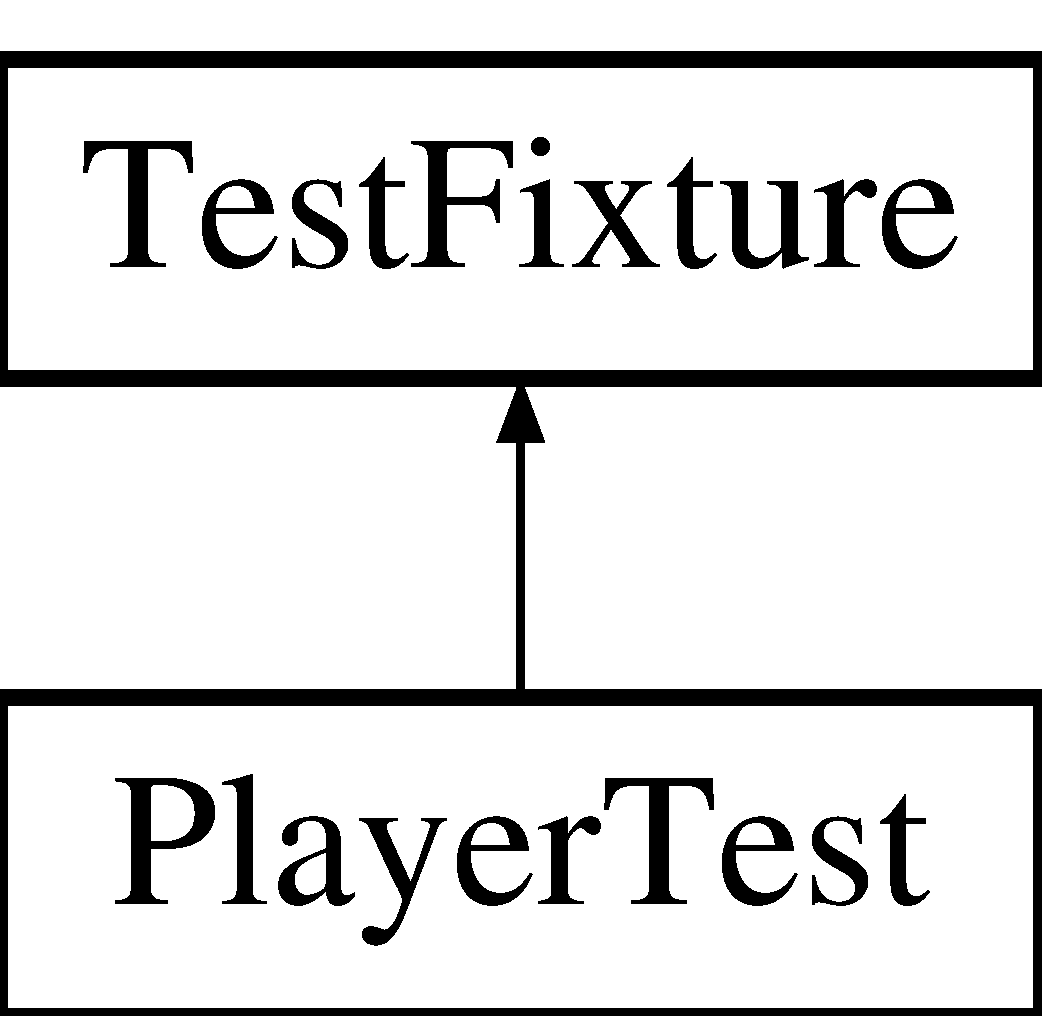
\includegraphics[height=2.000000cm]{classPlayerTest}
\end{center}
\end{figure}
\subsection*{Public Member Functions}
\begin{DoxyCompactItemize}
\item 
void \hyperlink{classPlayerTest_a5fc4e3940fe2442cc760b12985ceef3b}{set\-Up} ()
\item 
void \hyperlink{classPlayerTest_af7b63b181271a7fa168cf73b0d85d346}{Test\-Keys} ()
\begin{DoxyCompactList}\small\item\em $>$override {\ttfamily set\-Up} to create variable \end{DoxyCompactList}\end{DoxyCompactItemize}
\subsection*{Private Member Functions}
\begin{DoxyCompactItemize}
\item 
\hyperlink{classPlayerTest_a02dcdc23e12801f583826e13aa38609d}{C\-P\-P\-U\-N\-I\-T\-\_\-\-T\-E\-S\-T\-\_\-\-S\-U\-I\-T\-E} (\hyperlink{classPlayerTest}{Player\-Test})
\item 
\hyperlink{classPlayerTest_a0159eeaf95cc6bf3ddc352efd6049530}{C\-P\-P\-U\-N\-I\-T\-\_\-\-T\-E\-S\-T} (\hyperlink{classPlayerTest_af7b63b181271a7fa168cf73b0d85d346}{Test\-Keys})
\item 
\hyperlink{classPlayerTest_ae5022bed52c0af937d91f24e614d8ea6}{C\-P\-P\-U\-N\-I\-T\-\_\-\-T\-E\-S\-T\-\_\-\-S\-U\-I\-T\-E\-\_\-\-E\-N\-D} ()
\end{DoxyCompactItemize}
\subsection*{Private Attributes}
\begin{DoxyCompactItemize}
\item 
int \hyperlink{classPlayerTest_ae4e634b9de6e1a835fead6433fb68108}{key\-Mod}
\item 
\hyperlink{classPlayer}{Player} \hyperlink{classPlayerTest_aa4d4751434ca1508f9962ffc03c37447}{T}
\end{DoxyCompactItemize}


\subsection{Detailed Description}
class to test functionality of the Int\-Vector class 

\subsection{Member Function Documentation}
\hypertarget{classPlayerTest_a0159eeaf95cc6bf3ddc352efd6049530}{\index{Player\-Test@{Player\-Test}!C\-P\-P\-U\-N\-I\-T\-\_\-\-T\-E\-S\-T@{C\-P\-P\-U\-N\-I\-T\-\_\-\-T\-E\-S\-T}}
\index{C\-P\-P\-U\-N\-I\-T\-\_\-\-T\-E\-S\-T@{C\-P\-P\-U\-N\-I\-T\-\_\-\-T\-E\-S\-T}!PlayerTest@{Player\-Test}}
\subsubsection[{C\-P\-P\-U\-N\-I\-T\-\_\-\-T\-E\-S\-T}]{\setlength{\rightskip}{0pt plus 5cm}Player\-Test\-::\-C\-P\-P\-U\-N\-I\-T\-\_\-\-T\-E\-S\-T (
\begin{DoxyParamCaption}
\item[{{\bf Test\-Keys}}]{}
\end{DoxyParamCaption}
)\hspace{0.3cm}{\ttfamily [private]}}}\label{classPlayerTest_a0159eeaf95cc6bf3ddc352efd6049530}
\hypertarget{classPlayerTest_a02dcdc23e12801f583826e13aa38609d}{\index{Player\-Test@{Player\-Test}!C\-P\-P\-U\-N\-I\-T\-\_\-\-T\-E\-S\-T\-\_\-\-S\-U\-I\-T\-E@{C\-P\-P\-U\-N\-I\-T\-\_\-\-T\-E\-S\-T\-\_\-\-S\-U\-I\-T\-E}}
\index{C\-P\-P\-U\-N\-I\-T\-\_\-\-T\-E\-S\-T\-\_\-\-S\-U\-I\-T\-E@{C\-P\-P\-U\-N\-I\-T\-\_\-\-T\-E\-S\-T\-\_\-\-S\-U\-I\-T\-E}!PlayerTest@{Player\-Test}}
\subsubsection[{C\-P\-P\-U\-N\-I\-T\-\_\-\-T\-E\-S\-T\-\_\-\-S\-U\-I\-T\-E}]{\setlength{\rightskip}{0pt plus 5cm}Player\-Test\-::\-C\-P\-P\-U\-N\-I\-T\-\_\-\-T\-E\-S\-T\-\_\-\-S\-U\-I\-T\-E (
\begin{DoxyParamCaption}
\item[{{\bf Player\-Test}}]{}
\end{DoxyParamCaption}
)\hspace{0.3cm}{\ttfamily [private]}}}\label{classPlayerTest_a02dcdc23e12801f583826e13aa38609d}
\hypertarget{classPlayerTest_ae5022bed52c0af937d91f24e614d8ea6}{\index{Player\-Test@{Player\-Test}!C\-P\-P\-U\-N\-I\-T\-\_\-\-T\-E\-S\-T\-\_\-\-S\-U\-I\-T\-E\-\_\-\-E\-N\-D@{C\-P\-P\-U\-N\-I\-T\-\_\-\-T\-E\-S\-T\-\_\-\-S\-U\-I\-T\-E\-\_\-\-E\-N\-D}}
\index{C\-P\-P\-U\-N\-I\-T\-\_\-\-T\-E\-S\-T\-\_\-\-S\-U\-I\-T\-E\-\_\-\-E\-N\-D@{C\-P\-P\-U\-N\-I\-T\-\_\-\-T\-E\-S\-T\-\_\-\-S\-U\-I\-T\-E\-\_\-\-E\-N\-D}!PlayerTest@{Player\-Test}}
\subsubsection[{C\-P\-P\-U\-N\-I\-T\-\_\-\-T\-E\-S\-T\-\_\-\-S\-U\-I\-T\-E\-\_\-\-E\-N\-D}]{\setlength{\rightskip}{0pt plus 5cm}Player\-Test\-::\-C\-P\-P\-U\-N\-I\-T\-\_\-\-T\-E\-S\-T\-\_\-\-S\-U\-I\-T\-E\-\_\-\-E\-N\-D (
\begin{DoxyParamCaption}
{}
\end{DoxyParamCaption}
)\hspace{0.3cm}{\ttfamily [private]}}}\label{classPlayerTest_ae5022bed52c0af937d91f24e614d8ea6}
\hypertarget{classPlayerTest_a5fc4e3940fe2442cc760b12985ceef3b}{\index{Player\-Test@{Player\-Test}!set\-Up@{set\-Up}}
\index{set\-Up@{set\-Up}!PlayerTest@{Player\-Test}}
\subsubsection[{set\-Up}]{\setlength{\rightskip}{0pt plus 5cm}void Player\-Test\-::set\-Up (
\begin{DoxyParamCaption}
{}
\end{DoxyParamCaption}
)}}\label{classPlayerTest_a5fc4e3940fe2442cc760b12985ceef3b}
\hypertarget{classPlayerTest_af7b63b181271a7fa168cf73b0d85d346}{\index{Player\-Test@{Player\-Test}!Test\-Keys@{Test\-Keys}}
\index{Test\-Keys@{Test\-Keys}!PlayerTest@{Player\-Test}}
\subsubsection[{Test\-Keys}]{\setlength{\rightskip}{0pt plus 5cm}void Player\-Test\-::\-Test\-Keys (
\begin{DoxyParamCaption}
{}
\end{DoxyParamCaption}
)}}\label{classPlayerTest_af7b63b181271a7fa168cf73b0d85d346}


$>$override {\ttfamily set\-Up} to create variable 



\subsection{Member Data Documentation}
\hypertarget{classPlayerTest_ae4e634b9de6e1a835fead6433fb68108}{\index{Player\-Test@{Player\-Test}!key\-Mod@{key\-Mod}}
\index{key\-Mod@{key\-Mod}!PlayerTest@{Player\-Test}}
\subsubsection[{key\-Mod}]{\setlength{\rightskip}{0pt plus 5cm}int Player\-Test\-::key\-Mod\hspace{0.3cm}{\ttfamily [private]}}}\label{classPlayerTest_ae4e634b9de6e1a835fead6433fb68108}
\hypertarget{classPlayerTest_aa4d4751434ca1508f9962ffc03c37447}{\index{Player\-Test@{Player\-Test}!T@{T}}
\index{T@{T}!PlayerTest@{Player\-Test}}
\subsubsection[{T}]{\setlength{\rightskip}{0pt plus 5cm}{\bf Player} Player\-Test\-::\-T\hspace{0.3cm}{\ttfamily [private]}}}\label{classPlayerTest_aa4d4751434ca1508f9962ffc03c37447}


The documentation for this class was generated from the following files\-:\begin{DoxyCompactItemize}
\item 
/home/rigt2720/\-Kodika/\-Character/\hyperlink{PlayerTest_8h}{Player\-Test.\-h}\item 
/home/rigt2720/\-Kodika/\-Character/\hyperlink{PlayerTest_8cpp}{Player\-Test.\-cpp}\end{DoxyCompactItemize}

\hypertarget{classPuzzle}{\section{Puzzle Class Reference}
\label{classPuzzle}\index{Puzzle@{Puzzle}}
}


{\ttfamily \#include $<$Puzzle.\-h$>$}

Inheritance diagram for Puzzle\-:\begin{figure}[H]
\begin{center}
\leavevmode
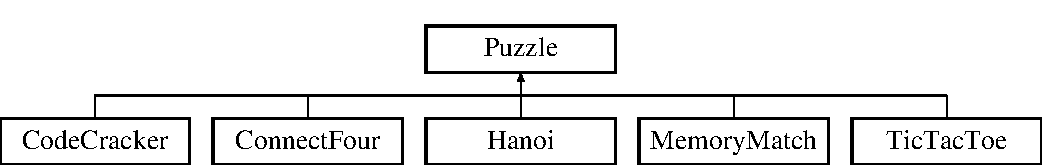
\includegraphics[height=2.000000cm]{classPuzzle}
\end{center}
\end{figure}
\subsection*{Public Member Functions}
\begin{DoxyCompactItemize}
\item 
int \hyperlink{classPuzzle_ad0be5c887460d0b386bf5d97264f0c24}{Random\-Number} (int n) const 
\item 
virtual \hyperlink{classPuzzle_a4319df1536a07cd1aaf23b27aeb53579}{$\sim$\-Puzzle} ()
\begin{DoxyCompactList}\small\item\em Virtual Destructor. \end{DoxyCompactList}\item 
virtual void \hyperlink{classPuzzle_a134875b96b18d9963d2b018fd14e7ab9}{Run\-Game} (\hyperlink{classCharacter}{Character} $\ast$player)=0
\end{DoxyCompactItemize}
\subsection*{Public Attributes}
\begin{DoxyCompactItemize}
\item 
bool \hyperlink{classPuzzle_a965ad54e9f7340c3cad944fc82c61a2b}{Puzzle\-End}
\begin{DoxyCompactList}\small\item\em Remains false until the mini-\/game/puzzle is ready to be terminated. \end{DoxyCompactList}\end{DoxyCompactItemize}
\subsection*{Private Member Functions}
\begin{DoxyCompactItemize}
\item 
virtual void \hyperlink{classPuzzle_adc90364342151caf536c4a34f2ca71d3}{Set\-Options\-In\-Menu} ()=0
\begin{DoxyCompactList}\small\item\em Sends the menu class the options for the player to select. \end{DoxyCompactList}\end{DoxyCompactItemize}


\subsection{Detailed Description}
\begin{DoxyAuthor}{Author}
Tyler Siwy 
\end{DoxyAuthor}
\begin{DoxyDate}{Date}
Oct 20, 2017\-This class represents an abstract base class for each mini-\/game/puzzle to derive from. 
\end{DoxyDate}


\subsection{Constructor \& Destructor Documentation}
\hypertarget{classPuzzle_a4319df1536a07cd1aaf23b27aeb53579}{\index{Puzzle@{Puzzle}!$\sim$\-Puzzle@{$\sim$\-Puzzle}}
\index{$\sim$\-Puzzle@{$\sim$\-Puzzle}!Puzzle@{Puzzle}}
\subsubsection[{$\sim$\-Puzzle}]{\setlength{\rightskip}{0pt plus 5cm}virtual Puzzle\-::$\sim$\-Puzzle (
\begin{DoxyParamCaption}
{}
\end{DoxyParamCaption}
)\hspace{0.3cm}{\ttfamily [inline]}, {\ttfamily [virtual]}}}\label{classPuzzle_a4319df1536a07cd1aaf23b27aeb53579}


Virtual Destructor. 



\subsection{Member Function Documentation}
\hypertarget{classPuzzle_ad0be5c887460d0b386bf5d97264f0c24}{\index{Puzzle@{Puzzle}!Random\-Number@{Random\-Number}}
\index{Random\-Number@{Random\-Number}!Puzzle@{Puzzle}}
\subsubsection[{Random\-Number}]{\setlength{\rightskip}{0pt plus 5cm}int Puzzle\-::\-Random\-Number (
\begin{DoxyParamCaption}
\item[{int}]{n}
\end{DoxyParamCaption}
) const}}\label{classPuzzle_ad0be5c887460d0b386bf5d97264f0c24}
Returns 0 to n-\/1 \hypertarget{classPuzzle_a134875b96b18d9963d2b018fd14e7ab9}{\index{Puzzle@{Puzzle}!Run\-Game@{Run\-Game}}
\index{Run\-Game@{Run\-Game}!Puzzle@{Puzzle}}
\subsubsection[{Run\-Game}]{\setlength{\rightskip}{0pt plus 5cm}virtual void Puzzle\-::\-Run\-Game (
\begin{DoxyParamCaption}
\item[{{\bf Character} $\ast$}]{player}
\end{DoxyParamCaption}
)\hspace{0.3cm}{\ttfamily [pure virtual]}}}\label{classPuzzle_a134875b96b18d9963d2b018fd14e7ab9}
Method to run the game, serves as a 'main' for the mini-\/game, calling functions from private until the player has won. 

Implemented in \hyperlink{classHanoi_a294a2a533b7f3305391aa880f7a0eb36}{Hanoi}, \hyperlink{classCodeCracker_a663fb6edb8141efd3b1760e46ea9f4e9}{Code\-Cracker}, \hyperlink{classTicTacToe_acf4f00b2f56781f0c41a4d51cfe03268}{Tic\-Tac\-Toe}, \hyperlink{classConnectFour_a3b578d1126bc575fa23b8811f121c8be}{Connect\-Four}, and \hyperlink{classMemoryMatch_a090950f764dee0b982ea254075d3667c}{Memory\-Match}.

\hypertarget{classPuzzle_adc90364342151caf536c4a34f2ca71d3}{\index{Puzzle@{Puzzle}!Set\-Options\-In\-Menu@{Set\-Options\-In\-Menu}}
\index{Set\-Options\-In\-Menu@{Set\-Options\-In\-Menu}!Puzzle@{Puzzle}}
\subsubsection[{Set\-Options\-In\-Menu}]{\setlength{\rightskip}{0pt plus 5cm}virtual void Puzzle\-::\-Set\-Options\-In\-Menu (
\begin{DoxyParamCaption}
{}
\end{DoxyParamCaption}
)\hspace{0.3cm}{\ttfamily [private]}, {\ttfamily [pure virtual]}}}\label{classPuzzle_adc90364342151caf536c4a34f2ca71d3}


Sends the menu class the options for the player to select. 

Does the appropriate action to the space selected by the user depending on which puzzle derived class it is being used in. 

Implemented in \hyperlink{classConnectFour_a58bd5328672a5c6d95fde740a4131eeb}{Connect\-Four}, \hyperlink{classCodeCracker_acbbd890be17cec27b879eb369de82017}{Code\-Cracker}, \hyperlink{classTicTacToe_a5fd34a83c96edbcf3c3c5a0930d513fb}{Tic\-Tac\-Toe}, \hyperlink{classHanoi_a4dd4c6028ade2b265ce98e48c3f2fb2a}{Hanoi}, and \hyperlink{classMemoryMatch_a62548d6cf028d372c08cc01a0693edb2}{Memory\-Match}.



\subsection{Member Data Documentation}
\hypertarget{classPuzzle_a965ad54e9f7340c3cad944fc82c61a2b}{\index{Puzzle@{Puzzle}!Puzzle\-End@{Puzzle\-End}}
\index{Puzzle\-End@{Puzzle\-End}!Puzzle@{Puzzle}}
\subsubsection[{Puzzle\-End}]{\setlength{\rightskip}{0pt plus 5cm}bool Puzzle\-::\-Puzzle\-End}}\label{classPuzzle_a965ad54e9f7340c3cad944fc82c61a2b}


Remains false until the mini-\/game/puzzle is ready to be terminated. 



The documentation for this class was generated from the following files\-:\begin{DoxyCompactItemize}
\item 
/home/rigt2720/\-Kodika/\-Puzzles/\hyperlink{Puzzle_8h}{Puzzle.\-h}\item 
/home/rigt2720/\-Kodika/\-Puzzles/\hyperlink{Puzzle_8cpp}{Puzzle.\-cpp}\end{DoxyCompactItemize}

\hypertarget{classPuzzleState}{\section{Puzzle\-State Class Reference}
\label{classPuzzleState}\index{Puzzle\-State@{Puzzle\-State}}
}


This is the state of the game when the player is interacting with a puzzle/minigame. Derived from \hyperlink{classGameState}{Game\-State}.  




{\ttfamily \#include $<$Puzzle\-State.\-h$>$}

Inheritance diagram for Puzzle\-State\-:\begin{figure}[H]
\begin{center}
\leavevmode
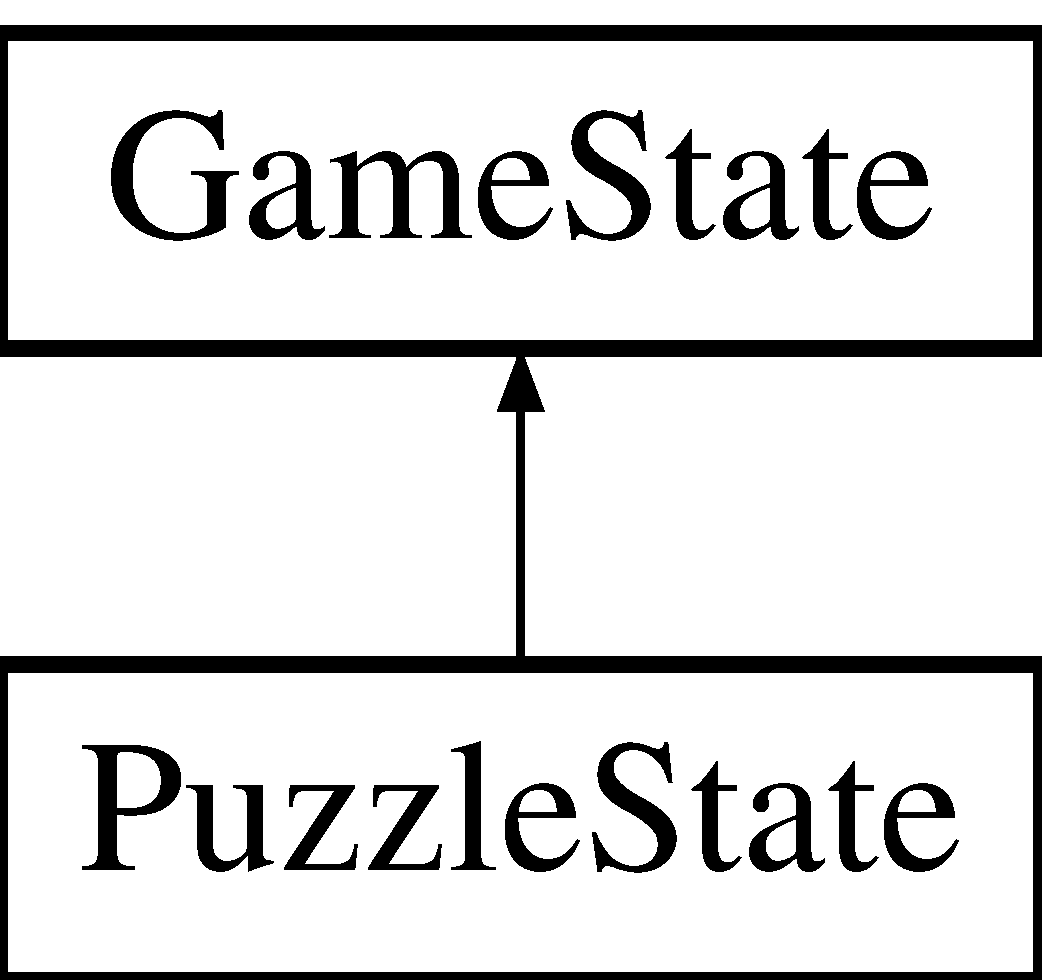
\includegraphics[height=2.000000cm]{classPuzzleState}
\end{center}
\end{figure}
\subsection*{Public Member Functions}
\begin{DoxyCompactItemize}
\item 
\hyperlink{classPuzzleState_a441deecdaf8b7ff103933664ff476870}{Puzzle\-State} ()
\begin{DoxyCompactList}\small\item\em Default constructor. \end{DoxyCompactList}\item 
void \hyperlink{classPuzzleState_a966b0f168ff5499f247c9ab519b524ab}{Set} ()
\begin{DoxyCompactList}\small\item\em Sets the layout of the game. \end{DoxyCompactList}\item 
void \hyperlink{classPuzzleState_ac9f6dd77d6471165d9eb2c18bd051dd1}{Get} ()
\begin{DoxyCompactList}\small\item\em Outputs the set layout. \end{DoxyCompactList}\end{DoxyCompactItemize}
\subsection*{Additional Inherited Members}


\subsection{Detailed Description}
This is the state of the game when the player is interacting with a puzzle/minigame. Derived from \hyperlink{classGameState}{Game\-State}. 

\begin{DoxyDate}{Date}
21/10/2017 
\end{DoxyDate}
\begin{DoxyAuthor}{Author}
Tomas Rigaux
\end{DoxyAuthor}
This is the state of the player when they are trying to solve a puzzle / minigame. 

\subsection{Constructor \& Destructor Documentation}
\hypertarget{classPuzzleState_a441deecdaf8b7ff103933664ff476870}{\index{Puzzle\-State@{Puzzle\-State}!Puzzle\-State@{Puzzle\-State}}
\index{Puzzle\-State@{Puzzle\-State}!PuzzleState@{Puzzle\-State}}
\subsubsection[{Puzzle\-State}]{\setlength{\rightskip}{0pt plus 5cm}Puzzle\-State\-::\-Puzzle\-State (
\begin{DoxyParamCaption}
{}
\end{DoxyParamCaption}
)}}\label{classPuzzleState_a441deecdaf8b7ff103933664ff476870}


Default constructor. 



\subsection{Member Function Documentation}
\hypertarget{classPuzzleState_ac9f6dd77d6471165d9eb2c18bd051dd1}{\index{Puzzle\-State@{Puzzle\-State}!Get@{Get}}
\index{Get@{Get}!PuzzleState@{Puzzle\-State}}
\subsubsection[{Get}]{\setlength{\rightskip}{0pt plus 5cm}void Puzzle\-State\-::\-Get (
\begin{DoxyParamCaption}
{}
\end{DoxyParamCaption}
)\hspace{0.3cm}{\ttfamily [virtual]}}}\label{classPuzzleState_ac9f6dd77d6471165d9eb2c18bd051dd1}


Outputs the set layout. 



Implements \hyperlink{classGameState_a4283cb3aa5637d4815d64272843a0625}{Game\-State}.

\hypertarget{classPuzzleState_a966b0f168ff5499f247c9ab519b524ab}{\index{Puzzle\-State@{Puzzle\-State}!Set@{Set}}
\index{Set@{Set}!PuzzleState@{Puzzle\-State}}
\subsubsection[{Set}]{\setlength{\rightskip}{0pt plus 5cm}void Puzzle\-State\-::\-Set (
\begin{DoxyParamCaption}
{}
\end{DoxyParamCaption}
)\hspace{0.3cm}{\ttfamily [virtual]}}}\label{classPuzzleState_a966b0f168ff5499f247c9ab519b524ab}


Sets the layout of the game. 



Implements \hyperlink{classGameState_af22e9a43999f99b784a35fab85cd9208}{Game\-State}.



The documentation for this class was generated from the following file\-:\begin{DoxyCompactItemize}
\item 
/home/rigt2720/\-Kodika/\-Game\-State/\hyperlink{PuzzleState_8h}{Puzzle\-State.\-h}\end{DoxyCompactItemize}

\hypertarget{classRiddleMenu}{\section{Riddle\-Menu Class Reference}
\label{classRiddleMenu}\index{Riddle\-Menu@{Riddle\-Menu}}
}


This is the menu class for the Riddle minigame.  




{\ttfamily \#include $<$Riddle\-Menu.\-h$>$}

Inheritance diagram for Riddle\-Menu\-:\begin{figure}[H]
\begin{center}
\leavevmode
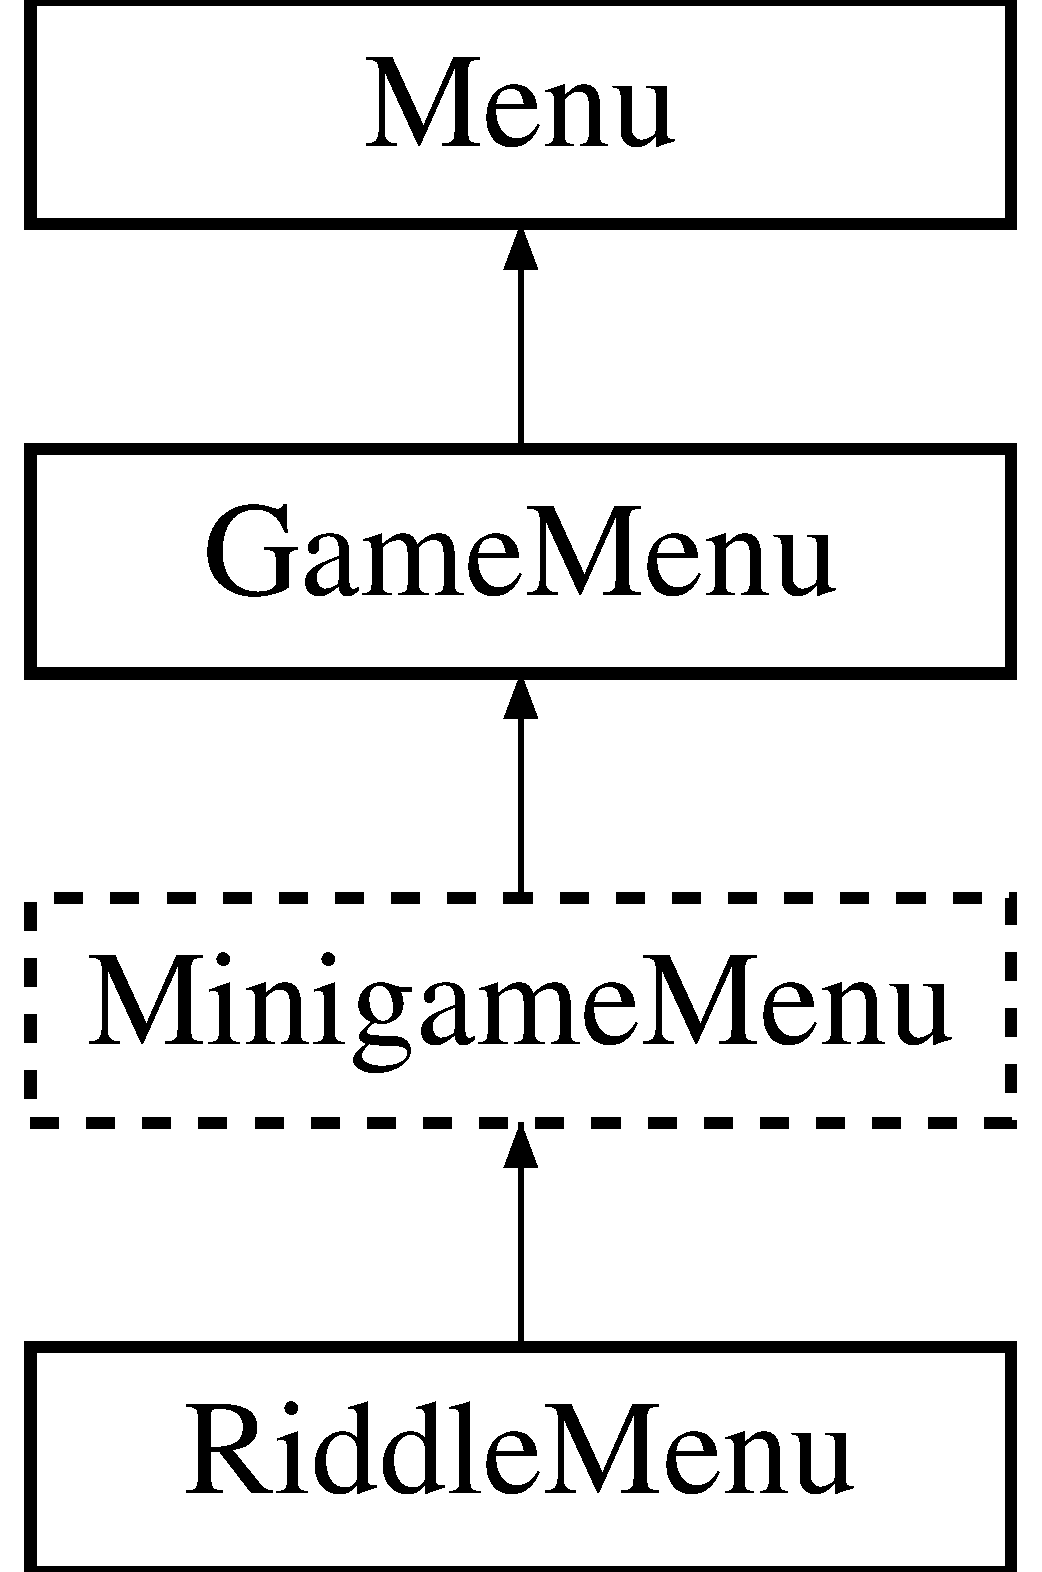
\includegraphics[height=4.000000cm]{classRiddleMenu}
\end{center}
\end{figure}
\subsection*{Public Member Functions}
\begin{DoxyCompactItemize}
\item 
\hyperlink{classRiddleMenu_a68e4be3bbc49bdb2f3d8a9fda74614d9}{Riddle\-Menu} ()
\begin{DoxyCompactList}\small\item\em This is the default constructor. \end{DoxyCompactList}\item 
virtual \hyperlink{classRiddleMenu_a9366deb179c1145947e37d599216d64e}{$\sim$\-Riddle\-Menu} ()
\begin{DoxyCompactList}\small\item\em This is the virtual destructor. \end{DoxyCompactList}\item 
virtual void \hyperlink{classRiddleMenu_a2d103283c58744ffa0e77e62a24e7ccb}{Set\-Options} (int row, int col, int space)
\item 
virtual void \hyperlink{classRiddleMenu_aef67f984c1aad0b8240e03b43ccbe615}{Handle\-Input} (istream \&is)
\item 
int \hyperlink{classRiddleMenu_a462f8a9d922e228c61619396e6ee8dc2}{Get\-Input} () const 
\begin{DoxyCompactList}\small\item\em Returns the players input to the riddle. \end{DoxyCompactList}\end{DoxyCompactItemize}
\subsection*{Private Attributes}
\begin{DoxyCompactItemize}
\item 
int \hyperlink{classRiddleMenu_a16feb2f9681e9753ff75363de2bf4bc3}{input}
\end{DoxyCompactItemize}
\subsection*{Additional Inherited Members}


\subsection{Detailed Description}
This is the menu class for the Riddle minigame. 

\subsection{Constructor \& Destructor Documentation}
\hypertarget{classRiddleMenu_a68e4be3bbc49bdb2f3d8a9fda74614d9}{\index{Riddle\-Menu@{Riddle\-Menu}!Riddle\-Menu@{Riddle\-Menu}}
\index{Riddle\-Menu@{Riddle\-Menu}!RiddleMenu@{Riddle\-Menu}}
\subsubsection[{Riddle\-Menu}]{\setlength{\rightskip}{0pt plus 5cm}Riddle\-Menu\-::\-Riddle\-Menu (
\begin{DoxyParamCaption}
{}
\end{DoxyParamCaption}
)}}\label{classRiddleMenu_a68e4be3bbc49bdb2f3d8a9fda74614d9}


This is the default constructor. 

\hypertarget{classRiddleMenu_a9366deb179c1145947e37d599216d64e}{\index{Riddle\-Menu@{Riddle\-Menu}!$\sim$\-Riddle\-Menu@{$\sim$\-Riddle\-Menu}}
\index{$\sim$\-Riddle\-Menu@{$\sim$\-Riddle\-Menu}!RiddleMenu@{Riddle\-Menu}}
\subsubsection[{$\sim$\-Riddle\-Menu}]{\setlength{\rightskip}{0pt plus 5cm}Riddle\-Menu\-::$\sim$\-Riddle\-Menu (
\begin{DoxyParamCaption}
{}
\end{DoxyParamCaption}
)\hspace{0.3cm}{\ttfamily [virtual]}}}\label{classRiddleMenu_a9366deb179c1145947e37d599216d64e}


This is the virtual destructor. 



\subsection{Member Function Documentation}
\hypertarget{classRiddleMenu_a462f8a9d922e228c61619396e6ee8dc2}{\index{Riddle\-Menu@{Riddle\-Menu}!Get\-Input@{Get\-Input}}
\index{Get\-Input@{Get\-Input}!RiddleMenu@{Riddle\-Menu}}
\subsubsection[{Get\-Input}]{\setlength{\rightskip}{0pt plus 5cm}int Riddle\-Menu\-::\-Get\-Input (
\begin{DoxyParamCaption}
{}
\end{DoxyParamCaption}
) const}}\label{classRiddleMenu_a462f8a9d922e228c61619396e6ee8dc2}


Returns the players input to the riddle. 

\hypertarget{classRiddleMenu_aef67f984c1aad0b8240e03b43ccbe615}{\index{Riddle\-Menu@{Riddle\-Menu}!Handle\-Input@{Handle\-Input}}
\index{Handle\-Input@{Handle\-Input}!RiddleMenu@{Riddle\-Menu}}
\subsubsection[{Handle\-Input}]{\setlength{\rightskip}{0pt plus 5cm}void Riddle\-Menu\-::\-Handle\-Input (
\begin{DoxyParamCaption}
\item[{istream \&}]{is}
\end{DoxyParamCaption}
)\hspace{0.3cm}{\ttfamily [virtual]}}}\label{classRiddleMenu_aef67f984c1aad0b8240e03b43ccbe615}
This function handles the input for the menu options. 
\begin{DoxyParams}[1]{Parameters}
\mbox{\tt in,out}  & {\em is} & The in-\/stream operator to read the input. \\
\hline
\end{DoxyParams}


Implements \hyperlink{classMinigameMenu_a3f854c4eefb0f3110cd085b3cfe56460}{Minigame\-Menu}.

\hypertarget{classRiddleMenu_a2d103283c58744ffa0e77e62a24e7ccb}{\index{Riddle\-Menu@{Riddle\-Menu}!Set\-Options@{Set\-Options}}
\index{Set\-Options@{Set\-Options}!RiddleMenu@{Riddle\-Menu}}
\subsubsection[{Set\-Options}]{\setlength{\rightskip}{0pt plus 5cm}void Riddle\-Menu\-::\-Set\-Options (
\begin{DoxyParamCaption}
\item[{int}]{row, }
\item[{int}]{col, }
\item[{int}]{space}
\end{DoxyParamCaption}
)\hspace{0.3cm}{\ttfamily [virtual]}}}\label{classRiddleMenu_a2d103283c58744ffa0e77e62a24e7ccb}
This function sets the specific options for the \hyperlink{classMenu}{Menu} type. 
\begin{DoxyParams}[1]{Parameters}
\mbox{\tt in}  & {\em row} & Determines which row the options will start being set at. \\
\hline
\mbox{\tt in}  & {\em col} & Determines which column the options will start from. \\
\hline
\mbox{\tt in}  & {\em How} & mush space inbetween rows. \\
\hline
\end{DoxyParams}


Implements \hyperlink{classMinigameMenu_abde3ae319bf1660a8626c6f765e054a8}{Minigame\-Menu}.



\subsection{Member Data Documentation}
\hypertarget{classRiddleMenu_a16feb2f9681e9753ff75363de2bf4bc3}{\index{Riddle\-Menu@{Riddle\-Menu}!input@{input}}
\index{input@{input}!RiddleMenu@{Riddle\-Menu}}
\subsubsection[{input}]{\setlength{\rightskip}{0pt plus 5cm}int Riddle\-Menu\-::input\hspace{0.3cm}{\ttfamily [private]}}}\label{classRiddleMenu_a16feb2f9681e9753ff75363de2bf4bc3}


The documentation for this class was generated from the following files\-:\begin{DoxyCompactItemize}
\item 
/home/rigt2720/\-Kodika/\-Menu/\hyperlink{RiddleMenu_8h}{Riddle\-Menu.\-h}\item 
/home/rigt2720/\-Kodika/\-Menu/\hyperlink{RiddleMenu_8cpp}{Riddle\-Menu.\-cpp}\end{DoxyCompactItemize}

\hypertarget{classRoom}{\section{Room Class Reference}
\label{classRoom}\index{Room@{Room}}
}


{\ttfamily \#include $<$Room.\-hh$>$}

\subsection*{Public Member Functions}
\begin{DoxyCompactItemize}
\item 
\hyperlink{classRoom_a755646673335862f28b57d5600b6fd30}{Room} (\hyperlink{classImage}{Image} \&img)
\item 
\hypertarget{classRoom_a67d5da09983cc53097807fd43ba5481a}{\hyperlink{classRoom_a67d5da09983cc53097807fd43ba5481a}{$\sim$\-Room} ()}\label{classRoom_a67d5da09983cc53097807fd43ba5481a}

\begin{DoxyCompactList}\small\item\em Destroys the object. \end{DoxyCompactList}\item 
void \hyperlink{classRoom_a267a11891afd9d608fd47f69c812f0e6}{Get\-Room} (vector$<$ \hyperlink{classImage}{Image} $\ast$ $>$ \&collection)
\item 
\hypertarget{classRoom_a74aefefa4c161799ca709a7f1d681ed2}{void \hyperlink{classRoom_a74aefefa4c161799ca709a7f1d681ed2}{Make\-Changes} ()}\label{classRoom_a74aefefa4c161799ca709a7f1d681ed2}

\begin{DoxyCompactList}\small\item\em Helper function to apply the images onto the room image. \end{DoxyCompactList}\item 
int \hyperlink{classRoom_a40f49471cbd82ece2b78cabbcd576a1f}{Randomizer} (int n)
\item 
\hypertarget{classRoom_ac7cd4e8afbc1de4dab38d0fad286aff8}{{\bfseries Room\-Tree} ()}\label{classRoom_ac7cd4e8afbc1de4dab38d0fad286aff8}

\item 
\hypertarget{classRoom_ae709e7bab6f0baef101a69f91c3f2494}{void {\bfseries new\-Room} (char dir)}\label{classRoom_ae709e7bab6f0baef101a69f91c3f2494}

\item 
\hypertarget{classRoom_aceaa2e1c7c1a8017d51434513a717c47}{void {\bfseries move} (char dir)}\label{classRoom_aceaa2e1c7c1a8017d51434513a717c47}

\item 
\hypertarget{classRoom_a3ce43bc6b9d2fd467160a807e07c8be2}{\hyperlink{classRoom}{Room} $\ast$ {\bfseries get\-Room} ()}\label{classRoom_a3ce43bc6b9d2fd467160a807e07c8be2}

\end{DoxyCompactItemize}


\subsection{Detailed Description}
The \hyperlink{classRoom}{Room} class defines random values that characterize a room's event. It also applies appropriate images onto a given room image 

\subsection{Constructor \& Destructor Documentation}
\hypertarget{classRoom_a755646673335862f28b57d5600b6fd30}{\index{Room@{Room}!Room@{Room}}
\index{Room@{Room}!Room@{Room}}
\subsubsection[{Room}]{\setlength{\rightskip}{0pt plus 5cm}Room\-::\-Room (
\begin{DoxyParamCaption}
\item[{{\bf Image} \&}]{img}
\end{DoxyParamCaption}
)}}\label{classRoom_a755646673335862f28b57d5600b6fd30}
Constructs a \hyperlink{classRoom}{Room} object using the given image 
\begin{DoxyParams}[1]{Parameters}
\mbox{\tt in}  & {\em img} & the image used as the room \\
\hline
\end{DoxyParams}


\subsection{Member Function Documentation}
\hypertarget{classRoom_a267a11891afd9d608fd47f69c812f0e6}{\index{Room@{Room}!Get\-Room@{Get\-Room}}
\index{Get\-Room@{Get\-Room}!Room@{Room}}
\subsubsection[{Get\-Room}]{\setlength{\rightskip}{0pt plus 5cm}void Room\-::\-Get\-Room (
\begin{DoxyParamCaption}
\item[{vector$<$ {\bf Image} $\ast$ $>$ \&}]{collection}
\end{DoxyParamCaption}
)}}\label{classRoom_a267a11891afd9d608fd47f69c812f0e6}
Constructs a \hyperlink{classRoom}{Room} object using the given image 
\begin{DoxyParams}[1]{Parameters}
\mbox{\tt in}  & {\em collection} & collects all 'event' images for the rooms \\
\hline
\end{DoxyParams}
\hypertarget{classRoom_a40f49471cbd82ece2b78cabbcd576a1f}{\index{Room@{Room}!Randomizer@{Randomizer}}
\index{Randomizer@{Randomizer}!Room@{Room}}
\subsubsection[{Randomizer}]{\setlength{\rightskip}{0pt plus 5cm}int Room\-::\-Randomizer (
\begin{DoxyParamCaption}
\item[{int}]{n}
\end{DoxyParamCaption}
)}}\label{classRoom_a40f49471cbd82ece2b78cabbcd576a1f}
Helper function to output a random value from 0 -\/ n 
\begin{DoxyParams}[1]{Parameters}
\mbox{\tt in}  & {\em n} & the range of the random number generated \\
\hline
\end{DoxyParams}


The documentation for this class was generated from the following files\-:\begin{DoxyCompactItemize}
\item 
Room/Room.\-hh\item 
Room\-Tree/Room\-Tree.\-h\end{DoxyCompactItemize}

\hypertarget{classRoomTree}{\section{Room\-Tree Class Reference}
\label{classRoomTree}\index{Room\-Tree@{Room\-Tree}}
}


Class to represent the layout of rooms in a doubly linked tree-\/like format.  




{\ttfamily \#include $<$Room\-Tree.\-h$>$}

\subsection*{Public Member Functions}
\begin{DoxyCompactItemize}
\item 
\hyperlink{classRoomTree_a2ea4adb06c7a1913d21ebaa6548a0167}{Room\-Tree} (\hyperlink{classRoom}{Room} $\ast$root\-Room)
\begin{DoxyCompactList}\small\item\em \hyperlink{classRoomTree}{Room\-Tree} Constructor. \end{DoxyCompactList}\item 
\hypertarget{classRoomTree_a1bd0bf9ba15d59e29127f762a3cdf036}{\hyperlink{classRoomTree_a1bd0bf9ba15d59e29127f762a3cdf036}{$\sim$\-Room\-Tree} ()}\label{classRoomTree_a1bd0bf9ba15d59e29127f762a3cdf036}

\begin{DoxyCompactList}\small\item\em \hyperlink{classRoomTree}{Room\-Tree} Destructor. \end{DoxyCompactList}\item 
void \hyperlink{classRoomTree_a198fd76507d341091eff6f9cb367d551}{new\-Room} (char dir, \hyperlink{classRoom}{Room} $\ast$roomptr)
\begin{DoxyCompactList}\small\item\em Inserts a new room at child (throws exeption if already occupied) \end{DoxyCompactList}\item 
bool \hyperlink{classRoomTree_af3d5ff5c2c7722186283c69c9519cd14}{move} (char dir)
\begin{DoxyCompactList}\small\item\em Moves current position through the tree. \end{DoxyCompactList}\item 
const \hyperlink{classRoom}{Room} $\ast$ \hyperlink{classRoomTree_a077743215ed41e741fd4106b3d285693}{at} () const 
\begin{DoxyCompactList}\small\item\em Gives a const pointer to the room currently at for accessing. \end{DoxyCompactList}\item 
\hyperlink{classRoom}{Room} $\ast$ \hyperlink{classRoomTree_abfad141f868410fa8c578d19f45eaa05}{at} ()
\begin{DoxyCompactList}\small\item\em Gives a pointer to the room currently at. \end{DoxyCompactList}\end{DoxyCompactItemize}


\subsection{Detailed Description}
Class to represent the layout of rooms in a doubly linked tree-\/like format. 

\subsection{Constructor \& Destructor Documentation}
\hypertarget{classRoomTree_a2ea4adb06c7a1913d21ebaa6548a0167}{\index{Room\-Tree@{Room\-Tree}!Room\-Tree@{Room\-Tree}}
\index{Room\-Tree@{Room\-Tree}!RoomTree@{Room\-Tree}}
\subsubsection[{Room\-Tree}]{\setlength{\rightskip}{0pt plus 5cm}Room\-Tree\-::\-Room\-Tree (
\begin{DoxyParamCaption}
\item[{{\bf Room} $\ast$}]{root\-Room}
\end{DoxyParamCaption}
)}}\label{classRoomTree_a2ea4adb06c7a1913d21ebaa6548a0167}


\hyperlink{classRoomTree}{Room\-Tree} Constructor. 

\hyperlink{classRoomTree}{Room\-Tree} Construtor. 

\subsection{Member Function Documentation}
\hypertarget{classRoomTree_a077743215ed41e741fd4106b3d285693}{\index{Room\-Tree@{Room\-Tree}!at@{at}}
\index{at@{at}!RoomTree@{Room\-Tree}}
\subsubsection[{at}]{\setlength{\rightskip}{0pt plus 5cm}const {\bf Room} $\ast$ Room\-Tree\-::at (
\begin{DoxyParamCaption}
{}
\end{DoxyParamCaption}
) const}}\label{classRoomTree_a077743215ed41e741fd4106b3d285693}


Gives a const pointer to the room currently at for accessing. 

Gives a const pointer to the room currently at for accessing \begin{DoxyReturn}{Returns}
A const pointer to current room 
\end{DoxyReturn}
\hypertarget{classRoomTree_abfad141f868410fa8c578d19f45eaa05}{\index{Room\-Tree@{Room\-Tree}!at@{at}}
\index{at@{at}!RoomTree@{Room\-Tree}}
\subsubsection[{at}]{\setlength{\rightskip}{0pt plus 5cm}{\bf Room} $\ast$ Room\-Tree\-::at (
\begin{DoxyParamCaption}
{}
\end{DoxyParamCaption}
)}}\label{classRoomTree_abfad141f868410fa8c578d19f45eaa05}


Gives a pointer to the room currently at. 

Gives a pointer to current room \begin{DoxyReturn}{Returns}
Pointer to current room 
\end{DoxyReturn}
\hypertarget{classRoomTree_af3d5ff5c2c7722186283c69c9519cd14}{\index{Room\-Tree@{Room\-Tree}!move@{move}}
\index{move@{move}!RoomTree@{Room\-Tree}}
\subsubsection[{move}]{\setlength{\rightskip}{0pt plus 5cm}bool Room\-Tree\-::move (
\begin{DoxyParamCaption}
\item[{char}]{dir}
\end{DoxyParamCaption}
)}}\label{classRoomTree_af3d5ff5c2c7722186283c69c9519cd14}


Moves current position through the tree. 

Moves through the tree 
\begin{DoxyParams}[1]{Parameters}
\mbox{\tt in}  & {\em dir} & Direction to move(left(l) right(r) center(c) or parent(p)) \\
\hline
\end{DoxyParams}
\begin{DoxyReturn}{Returns}
True if move was successfull, false otherwise 
\end{DoxyReturn}

\begin{DoxyExceptions}{Exceptions}
{\em invalid\-\_\-argument} & Thrown if the direction is invalid \\
\hline
{\em out\-\_\-of\-\_\-range} & Thrown if trying to move to the parent of the root \\
\hline
\end{DoxyExceptions}
\hypertarget{classRoomTree_a198fd76507d341091eff6f9cb367d551}{\index{Room\-Tree@{Room\-Tree}!new\-Room@{new\-Room}}
\index{new\-Room@{new\-Room}!RoomTree@{Room\-Tree}}
\subsubsection[{new\-Room}]{\setlength{\rightskip}{0pt plus 5cm}void Room\-Tree\-::new\-Room (
\begin{DoxyParamCaption}
\item[{char}]{dir, }
\item[{{\bf Room} $\ast$}]{roomptr}
\end{DoxyParamCaption}
)}}\label{classRoomTree_a198fd76507d341091eff6f9cb367d551}


Inserts a new room at child (throws exeption if already occupied) 

Inserts a new room at child (throws exeption if already occupied) 
\begin{DoxyParams}[1]{Parameters}
\mbox{\tt in}  & {\em dir} & Direction of the new child (left(l) right(r) or center(c)) \\
\hline
\end{DoxyParams}

\begin{DoxyExceptions}{Exceptions}
{\em invalid\-\_\-argument} & Thrown if the direction is invalid or space is occupied \\
\hline
\end{DoxyExceptions}


The documentation for this class was generated from the following files\-:\begin{DoxyCompactItemize}
\item 
Room\-Tree/Room\-Tree.\-h\item 
Room\-Tree/Room\-Tree.\-cpp\end{DoxyCompactItemize}

\hypertarget{classRoomTreeTest}{\section{Room\-Tree\-Test Class Reference}
\label{classRoomTreeTest}\index{Room\-Tree\-Test@{Room\-Tree\-Test}}
}


Class that tests functionality of \hyperlink{classRoomTree}{Room\-Tree} Class.  




{\ttfamily \#include $<$Room\-Tree\-Test.\-h$>$}

Inheritance diagram for Room\-Tree\-Test\-:\begin{figure}[H]
\begin{center}
\leavevmode
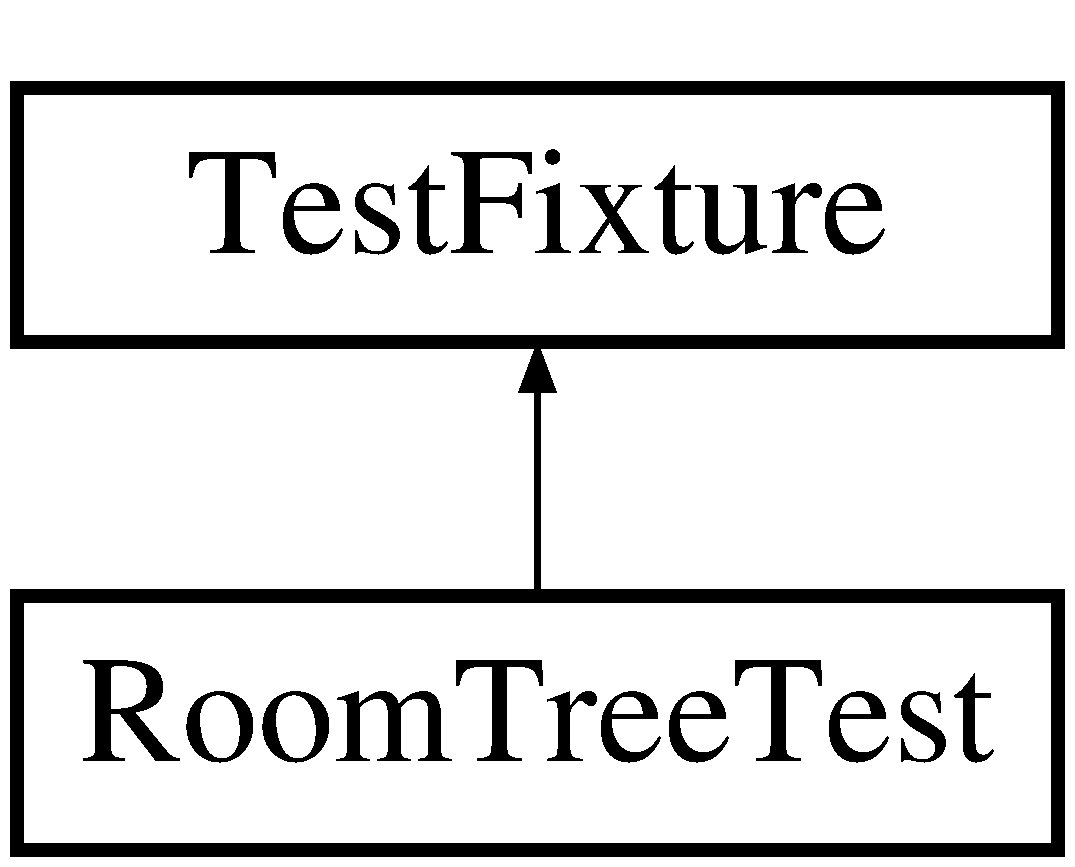
\includegraphics[height=2.000000cm]{classRoomTreeTest}
\end{center}
\end{figure}
\subsection*{Public Member Functions}
\begin{DoxyCompactItemize}
\item 
void \hyperlink{classRoomTreeTest_ae70ed88d72b79d6615705caf5a635aca}{set\-Up} ()
\begin{DoxyCompactList}\small\item\em Sets up tests for \hyperlink{classRoomTree}{Room\-Tree}. \end{DoxyCompactList}\item 
void \hyperlink{classRoomTreeTest_afa7584edb8a8267c922160e4d7c9d037}{tear\-Down} ()
\begin{DoxyCompactList}\small\item\em Cleans up tests. \end{DoxyCompactList}\item 
void \hyperlink{classRoomTreeTest_aab3dedfa3aaa0bfab811a8d0d8c8b7e0}{test\-Move} ()
\begin{DoxyCompactList}\small\item\em Tests the move Function. \end{DoxyCompactList}\item 
void \hyperlink{classRoomTreeTest_a1f342a990eb4b60cfae96dac1dbbedee}{test\-New\-Room} ()
\begin{DoxyCompactList}\small\item\em Tests the new\-Room Function. \end{DoxyCompactList}\item 
void \hyperlink{classRoomTreeTest_a7999cf9d9149ade6f39fbb7be601805e}{test\-At} ()
\begin{DoxyCompactList}\small\item\em Tests the at Function. \end{DoxyCompactList}\item 
void \hyperlink{classRoomTreeTest_a67dd37f922aabba4fefe925cfbd8483a}{test\-Current\-Height} ()
\begin{DoxyCompactList}\small\item\em Tests the Current\-Height function. \end{DoxyCompactList}\item 
void \hyperlink{classRoomTreeTest_a59d8363440d55c68ef79109efe88a5f5}{test\-Total\-Nodes} ()
\begin{DoxyCompactList}\small\item\em Tests the Total\-Nodes function. \end{DoxyCompactList}\end{DoxyCompactItemize}
\subsection*{Private Member Functions}
\begin{DoxyCompactItemize}
\item 
\hyperlink{classRoomTreeTest_a38df4c66be0d341a6d12fda7fdd1d6a4}{C\-P\-P\-U\-N\-I\-T\-\_\-\-T\-E\-S\-T\-\_\-\-S\-U\-I\-T\-E} (\hyperlink{classRoomTreeTest}{Room\-Tree\-Test})
\begin{DoxyCompactList}\small\item\em test suite macros \end{DoxyCompactList}\item 
\hyperlink{classRoomTreeTest_a0036ded2c0eebf44f7efe33a6599191e}{C\-P\-P\-U\-N\-I\-T\-\_\-\-T\-E\-S\-T} (\hyperlink{classRoomTreeTest_aab3dedfa3aaa0bfab811a8d0d8c8b7e0}{test\-Move})
\item 
\hyperlink{classRoomTreeTest_a3e253c371a946e2bc196ac4c83023c21}{C\-P\-P\-U\-N\-I\-T\-\_\-\-T\-E\-S\-T} (\hyperlink{classRoomTreeTest_a1f342a990eb4b60cfae96dac1dbbedee}{test\-New\-Room})
\item 
\hyperlink{classRoomTreeTest_a0eac4e16bb37465e894eb1a6ad74900e}{C\-P\-P\-U\-N\-I\-T\-\_\-\-T\-E\-S\-T} (\hyperlink{classRoomTreeTest_a7999cf9d9149ade6f39fbb7be601805e}{test\-At})
\item 
\hyperlink{classRoomTreeTest_a15f3666905d1c207aa1f90b445cb6f7f}{C\-P\-P\-U\-N\-I\-T\-\_\-\-T\-E\-S\-T} (\hyperlink{classRoomTreeTest_a67dd37f922aabba4fefe925cfbd8483a}{test\-Current\-Height})
\item 
\hyperlink{classRoomTreeTest_aa665ae61a669fecbdc3db4cb06c47767}{C\-P\-P\-U\-N\-I\-T\-\_\-\-T\-E\-S\-T} (\hyperlink{classRoomTreeTest_a59d8363440d55c68ef79109efe88a5f5}{test\-Total\-Nodes})
\item 
\hyperlink{classRoomTreeTest_a22c287ede74b7fc2591ceee86d10d85a}{C\-P\-P\-U\-N\-I\-T\-\_\-\-T\-E\-S\-T\-\_\-\-S\-U\-I\-T\-E\-\_\-\-E\-N\-D} ()
\end{DoxyCompactItemize}
\subsection*{Private Attributes}
\begin{DoxyCompactItemize}
\item 
\hyperlink{classRoomTree}{Room\-Tree} $\ast$ \hyperlink{classRoomTreeTest_aba5c37d20a82bff695de4c78a547f23f}{Tree1}
\item 
\hyperlink{classRoomTree}{Room\-Tree} $\ast$ \hyperlink{classRoomTreeTest_aada805154b8f5306805936f0ba43834c}{Tree2}
\item 
\hyperlink{classRoomTree}{Room\-Tree} $\ast$ \hyperlink{classRoomTreeTest_aa70878ec1fa44e95f78e59a236572b27}{Tree3}
\end{DoxyCompactItemize}


\subsection{Detailed Description}
Class that tests functionality of \hyperlink{classRoomTree}{Room\-Tree} Class. 

\subsection{Member Function Documentation}
\hypertarget{classRoomTreeTest_a0036ded2c0eebf44f7efe33a6599191e}{\index{Room\-Tree\-Test@{Room\-Tree\-Test}!C\-P\-P\-U\-N\-I\-T\-\_\-\-T\-E\-S\-T@{C\-P\-P\-U\-N\-I\-T\-\_\-\-T\-E\-S\-T}}
\index{C\-P\-P\-U\-N\-I\-T\-\_\-\-T\-E\-S\-T@{C\-P\-P\-U\-N\-I\-T\-\_\-\-T\-E\-S\-T}!RoomTreeTest@{Room\-Tree\-Test}}
\subsubsection[{C\-P\-P\-U\-N\-I\-T\-\_\-\-T\-E\-S\-T}]{\setlength{\rightskip}{0pt plus 5cm}Room\-Tree\-Test\-::\-C\-P\-P\-U\-N\-I\-T\-\_\-\-T\-E\-S\-T (
\begin{DoxyParamCaption}
\item[{{\bf test\-Move}}]{}
\end{DoxyParamCaption}
)\hspace{0.3cm}{\ttfamily [private]}}}\label{classRoomTreeTest_a0036ded2c0eebf44f7efe33a6599191e}
\hypertarget{classRoomTreeTest_a3e253c371a946e2bc196ac4c83023c21}{\index{Room\-Tree\-Test@{Room\-Tree\-Test}!C\-P\-P\-U\-N\-I\-T\-\_\-\-T\-E\-S\-T@{C\-P\-P\-U\-N\-I\-T\-\_\-\-T\-E\-S\-T}}
\index{C\-P\-P\-U\-N\-I\-T\-\_\-\-T\-E\-S\-T@{C\-P\-P\-U\-N\-I\-T\-\_\-\-T\-E\-S\-T}!RoomTreeTest@{Room\-Tree\-Test}}
\subsubsection[{C\-P\-P\-U\-N\-I\-T\-\_\-\-T\-E\-S\-T}]{\setlength{\rightskip}{0pt plus 5cm}Room\-Tree\-Test\-::\-C\-P\-P\-U\-N\-I\-T\-\_\-\-T\-E\-S\-T (
\begin{DoxyParamCaption}
\item[{{\bf test\-New\-Room}}]{}
\end{DoxyParamCaption}
)\hspace{0.3cm}{\ttfamily [private]}}}\label{classRoomTreeTest_a3e253c371a946e2bc196ac4c83023c21}
\hypertarget{classRoomTreeTest_a0eac4e16bb37465e894eb1a6ad74900e}{\index{Room\-Tree\-Test@{Room\-Tree\-Test}!C\-P\-P\-U\-N\-I\-T\-\_\-\-T\-E\-S\-T@{C\-P\-P\-U\-N\-I\-T\-\_\-\-T\-E\-S\-T}}
\index{C\-P\-P\-U\-N\-I\-T\-\_\-\-T\-E\-S\-T@{C\-P\-P\-U\-N\-I\-T\-\_\-\-T\-E\-S\-T}!RoomTreeTest@{Room\-Tree\-Test}}
\subsubsection[{C\-P\-P\-U\-N\-I\-T\-\_\-\-T\-E\-S\-T}]{\setlength{\rightskip}{0pt plus 5cm}Room\-Tree\-Test\-::\-C\-P\-P\-U\-N\-I\-T\-\_\-\-T\-E\-S\-T (
\begin{DoxyParamCaption}
\item[{{\bf test\-At}}]{}
\end{DoxyParamCaption}
)\hspace{0.3cm}{\ttfamily [private]}}}\label{classRoomTreeTest_a0eac4e16bb37465e894eb1a6ad74900e}
\hypertarget{classRoomTreeTest_a15f3666905d1c207aa1f90b445cb6f7f}{\index{Room\-Tree\-Test@{Room\-Tree\-Test}!C\-P\-P\-U\-N\-I\-T\-\_\-\-T\-E\-S\-T@{C\-P\-P\-U\-N\-I\-T\-\_\-\-T\-E\-S\-T}}
\index{C\-P\-P\-U\-N\-I\-T\-\_\-\-T\-E\-S\-T@{C\-P\-P\-U\-N\-I\-T\-\_\-\-T\-E\-S\-T}!RoomTreeTest@{Room\-Tree\-Test}}
\subsubsection[{C\-P\-P\-U\-N\-I\-T\-\_\-\-T\-E\-S\-T}]{\setlength{\rightskip}{0pt plus 5cm}Room\-Tree\-Test\-::\-C\-P\-P\-U\-N\-I\-T\-\_\-\-T\-E\-S\-T (
\begin{DoxyParamCaption}
\item[{{\bf test\-Current\-Height}}]{}
\end{DoxyParamCaption}
)\hspace{0.3cm}{\ttfamily [private]}}}\label{classRoomTreeTest_a15f3666905d1c207aa1f90b445cb6f7f}
\hypertarget{classRoomTreeTest_aa665ae61a669fecbdc3db4cb06c47767}{\index{Room\-Tree\-Test@{Room\-Tree\-Test}!C\-P\-P\-U\-N\-I\-T\-\_\-\-T\-E\-S\-T@{C\-P\-P\-U\-N\-I\-T\-\_\-\-T\-E\-S\-T}}
\index{C\-P\-P\-U\-N\-I\-T\-\_\-\-T\-E\-S\-T@{C\-P\-P\-U\-N\-I\-T\-\_\-\-T\-E\-S\-T}!RoomTreeTest@{Room\-Tree\-Test}}
\subsubsection[{C\-P\-P\-U\-N\-I\-T\-\_\-\-T\-E\-S\-T}]{\setlength{\rightskip}{0pt plus 5cm}Room\-Tree\-Test\-::\-C\-P\-P\-U\-N\-I\-T\-\_\-\-T\-E\-S\-T (
\begin{DoxyParamCaption}
\item[{{\bf test\-Total\-Nodes}}]{}
\end{DoxyParamCaption}
)\hspace{0.3cm}{\ttfamily [private]}}}\label{classRoomTreeTest_aa665ae61a669fecbdc3db4cb06c47767}
\hypertarget{classRoomTreeTest_a38df4c66be0d341a6d12fda7fdd1d6a4}{\index{Room\-Tree\-Test@{Room\-Tree\-Test}!C\-P\-P\-U\-N\-I\-T\-\_\-\-T\-E\-S\-T\-\_\-\-S\-U\-I\-T\-E@{C\-P\-P\-U\-N\-I\-T\-\_\-\-T\-E\-S\-T\-\_\-\-S\-U\-I\-T\-E}}
\index{C\-P\-P\-U\-N\-I\-T\-\_\-\-T\-E\-S\-T\-\_\-\-S\-U\-I\-T\-E@{C\-P\-P\-U\-N\-I\-T\-\_\-\-T\-E\-S\-T\-\_\-\-S\-U\-I\-T\-E}!RoomTreeTest@{Room\-Tree\-Test}}
\subsubsection[{C\-P\-P\-U\-N\-I\-T\-\_\-\-T\-E\-S\-T\-\_\-\-S\-U\-I\-T\-E}]{\setlength{\rightskip}{0pt plus 5cm}Room\-Tree\-Test\-::\-C\-P\-P\-U\-N\-I\-T\-\_\-\-T\-E\-S\-T\-\_\-\-S\-U\-I\-T\-E (
\begin{DoxyParamCaption}
\item[{{\bf Room\-Tree\-Test}}]{}
\end{DoxyParamCaption}
)\hspace{0.3cm}{\ttfamily [private]}}}\label{classRoomTreeTest_a38df4c66be0d341a6d12fda7fdd1d6a4}


test suite macros 

\hypertarget{classRoomTreeTest_a22c287ede74b7fc2591ceee86d10d85a}{\index{Room\-Tree\-Test@{Room\-Tree\-Test}!C\-P\-P\-U\-N\-I\-T\-\_\-\-T\-E\-S\-T\-\_\-\-S\-U\-I\-T\-E\-\_\-\-E\-N\-D@{C\-P\-P\-U\-N\-I\-T\-\_\-\-T\-E\-S\-T\-\_\-\-S\-U\-I\-T\-E\-\_\-\-E\-N\-D}}
\index{C\-P\-P\-U\-N\-I\-T\-\_\-\-T\-E\-S\-T\-\_\-\-S\-U\-I\-T\-E\-\_\-\-E\-N\-D@{C\-P\-P\-U\-N\-I\-T\-\_\-\-T\-E\-S\-T\-\_\-\-S\-U\-I\-T\-E\-\_\-\-E\-N\-D}!RoomTreeTest@{Room\-Tree\-Test}}
\subsubsection[{C\-P\-P\-U\-N\-I\-T\-\_\-\-T\-E\-S\-T\-\_\-\-S\-U\-I\-T\-E\-\_\-\-E\-N\-D}]{\setlength{\rightskip}{0pt plus 5cm}Room\-Tree\-Test\-::\-C\-P\-P\-U\-N\-I\-T\-\_\-\-T\-E\-S\-T\-\_\-\-S\-U\-I\-T\-E\-\_\-\-E\-N\-D (
\begin{DoxyParamCaption}
{}
\end{DoxyParamCaption}
)\hspace{0.3cm}{\ttfamily [private]}}}\label{classRoomTreeTest_a22c287ede74b7fc2591ceee86d10d85a}
\hypertarget{classRoomTreeTest_ae70ed88d72b79d6615705caf5a635aca}{\index{Room\-Tree\-Test@{Room\-Tree\-Test}!set\-Up@{set\-Up}}
\index{set\-Up@{set\-Up}!RoomTreeTest@{Room\-Tree\-Test}}
\subsubsection[{set\-Up}]{\setlength{\rightskip}{0pt plus 5cm}void Room\-Tree\-Test\-::set\-Up (
\begin{DoxyParamCaption}
{}
\end{DoxyParamCaption}
)}}\label{classRoomTreeTest_ae70ed88d72b79d6615705caf5a635aca}


Sets up tests for \hyperlink{classRoomTree}{Room\-Tree}. 

\hypertarget{classRoomTreeTest_afa7584edb8a8267c922160e4d7c9d037}{\index{Room\-Tree\-Test@{Room\-Tree\-Test}!tear\-Down@{tear\-Down}}
\index{tear\-Down@{tear\-Down}!RoomTreeTest@{Room\-Tree\-Test}}
\subsubsection[{tear\-Down}]{\setlength{\rightskip}{0pt plus 5cm}void Room\-Tree\-Test\-::tear\-Down (
\begin{DoxyParamCaption}
{}
\end{DoxyParamCaption}
)}}\label{classRoomTreeTest_afa7584edb8a8267c922160e4d7c9d037}


Cleans up tests. 

\hypertarget{classRoomTreeTest_a7999cf9d9149ade6f39fbb7be601805e}{\index{Room\-Tree\-Test@{Room\-Tree\-Test}!test\-At@{test\-At}}
\index{test\-At@{test\-At}!RoomTreeTest@{Room\-Tree\-Test}}
\subsubsection[{test\-At}]{\setlength{\rightskip}{0pt plus 5cm}void Room\-Tree\-Test\-::test\-At (
\begin{DoxyParamCaption}
{}
\end{DoxyParamCaption}
)}}\label{classRoomTreeTest_a7999cf9d9149ade6f39fbb7be601805e}


Tests the at Function. 

\hypertarget{classRoomTreeTest_a67dd37f922aabba4fefe925cfbd8483a}{\index{Room\-Tree\-Test@{Room\-Tree\-Test}!test\-Current\-Height@{test\-Current\-Height}}
\index{test\-Current\-Height@{test\-Current\-Height}!RoomTreeTest@{Room\-Tree\-Test}}
\subsubsection[{test\-Current\-Height}]{\setlength{\rightskip}{0pt plus 5cm}void Room\-Tree\-Test\-::test\-Current\-Height (
\begin{DoxyParamCaption}
{}
\end{DoxyParamCaption}
)}}\label{classRoomTreeTest_a67dd37f922aabba4fefe925cfbd8483a}


Tests the Current\-Height function. 

\hypertarget{classRoomTreeTest_aab3dedfa3aaa0bfab811a8d0d8c8b7e0}{\index{Room\-Tree\-Test@{Room\-Tree\-Test}!test\-Move@{test\-Move}}
\index{test\-Move@{test\-Move}!RoomTreeTest@{Room\-Tree\-Test}}
\subsubsection[{test\-Move}]{\setlength{\rightskip}{0pt plus 5cm}void Room\-Tree\-Test\-::test\-Move (
\begin{DoxyParamCaption}
{}
\end{DoxyParamCaption}
)}}\label{classRoomTreeTest_aab3dedfa3aaa0bfab811a8d0d8c8b7e0}


Tests the move Function. 

\hypertarget{classRoomTreeTest_a1f342a990eb4b60cfae96dac1dbbedee}{\index{Room\-Tree\-Test@{Room\-Tree\-Test}!test\-New\-Room@{test\-New\-Room}}
\index{test\-New\-Room@{test\-New\-Room}!RoomTreeTest@{Room\-Tree\-Test}}
\subsubsection[{test\-New\-Room}]{\setlength{\rightskip}{0pt plus 5cm}void Room\-Tree\-Test\-::test\-New\-Room (
\begin{DoxyParamCaption}
{}
\end{DoxyParamCaption}
)}}\label{classRoomTreeTest_a1f342a990eb4b60cfae96dac1dbbedee}


Tests the new\-Room Function. 

\hypertarget{classRoomTreeTest_a59d8363440d55c68ef79109efe88a5f5}{\index{Room\-Tree\-Test@{Room\-Tree\-Test}!test\-Total\-Nodes@{test\-Total\-Nodes}}
\index{test\-Total\-Nodes@{test\-Total\-Nodes}!RoomTreeTest@{Room\-Tree\-Test}}
\subsubsection[{test\-Total\-Nodes}]{\setlength{\rightskip}{0pt plus 5cm}void Room\-Tree\-Test\-::test\-Total\-Nodes (
\begin{DoxyParamCaption}
{}
\end{DoxyParamCaption}
)}}\label{classRoomTreeTest_a59d8363440d55c68ef79109efe88a5f5}


Tests the Total\-Nodes function. 



\subsection{Member Data Documentation}
\hypertarget{classRoomTreeTest_aba5c37d20a82bff695de4c78a547f23f}{\index{Room\-Tree\-Test@{Room\-Tree\-Test}!Tree1@{Tree1}}
\index{Tree1@{Tree1}!RoomTreeTest@{Room\-Tree\-Test}}
\subsubsection[{Tree1}]{\setlength{\rightskip}{0pt plus 5cm}{\bf Room\-Tree}$\ast$ Room\-Tree\-Test\-::\-Tree1\hspace{0.3cm}{\ttfamily [private]}}}\label{classRoomTreeTest_aba5c37d20a82bff695de4c78a547f23f}
\hypertarget{classRoomTreeTest_aada805154b8f5306805936f0ba43834c}{\index{Room\-Tree\-Test@{Room\-Tree\-Test}!Tree2@{Tree2}}
\index{Tree2@{Tree2}!RoomTreeTest@{Room\-Tree\-Test}}
\subsubsection[{Tree2}]{\setlength{\rightskip}{0pt plus 5cm}{\bf Room\-Tree}$\ast$ Room\-Tree\-Test\-::\-Tree2\hspace{0.3cm}{\ttfamily [private]}}}\label{classRoomTreeTest_aada805154b8f5306805936f0ba43834c}
\hypertarget{classRoomTreeTest_aa70878ec1fa44e95f78e59a236572b27}{\index{Room\-Tree\-Test@{Room\-Tree\-Test}!Tree3@{Tree3}}
\index{Tree3@{Tree3}!RoomTreeTest@{Room\-Tree\-Test}}
\subsubsection[{Tree3}]{\setlength{\rightskip}{0pt plus 5cm}{\bf Room\-Tree}$\ast$ Room\-Tree\-Test\-::\-Tree3\hspace{0.3cm}{\ttfamily [private]}}}\label{classRoomTreeTest_aa70878ec1fa44e95f78e59a236572b27}


The documentation for this class was generated from the following files\-:\begin{DoxyCompactItemize}
\item 
/home/rigt2720/\-Kodika/\-Room\-Tree/\hyperlink{RoomTreeTest_8h}{Room\-Tree\-Test.\-h}\item 
/home/rigt2720/\-Kodika/\-Room\-Tree/\hyperlink{RoomTreeTest_8cpp}{Room\-Tree\-Test.\-cpp}\end{DoxyCompactItemize}

\hypertarget{classScreen}{\section{Screen Class Reference}
\label{classScreen}\index{Screen@{Screen}}
}


{\ttfamily \#include $<$Screen.\-h$>$}

Inheritance diagram for Screen\-:\begin{figure}[H]
\begin{center}
\leavevmode
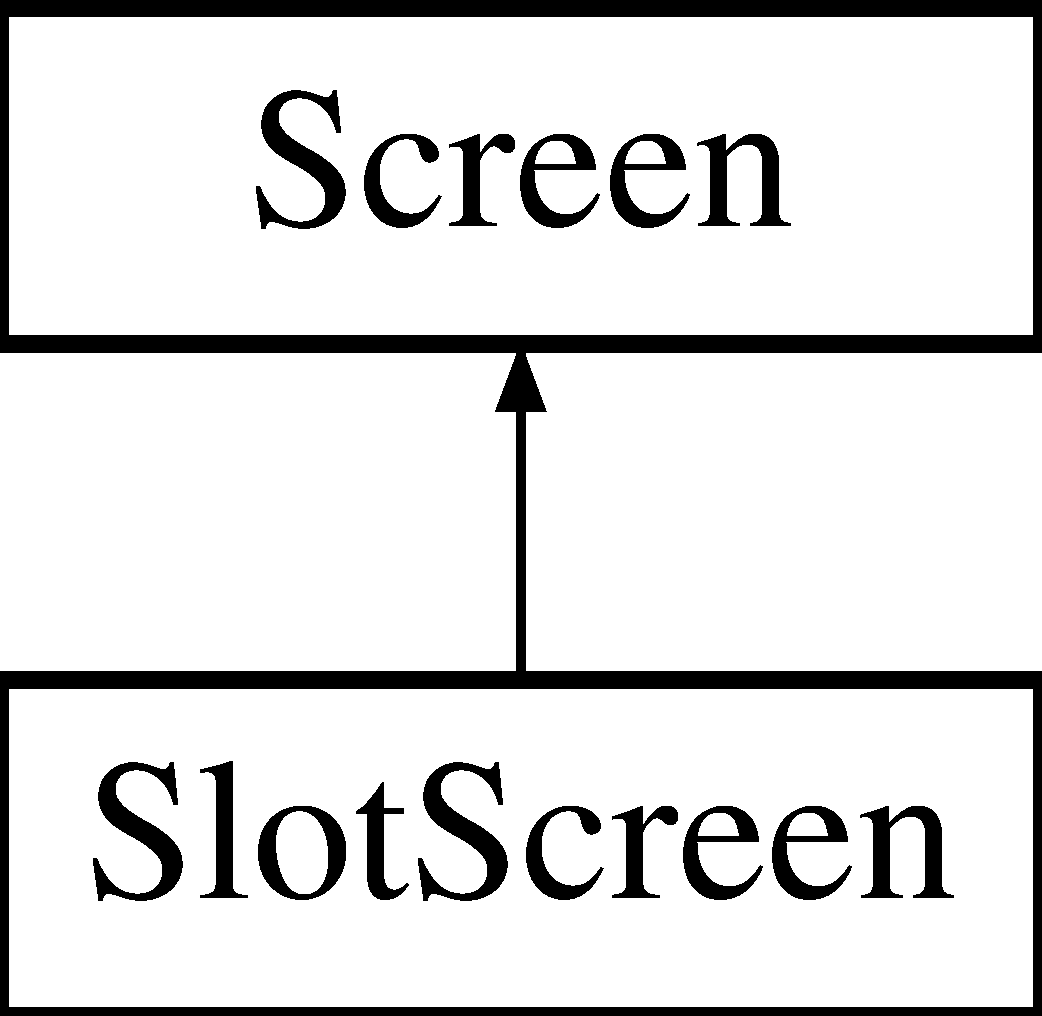
\includegraphics[height=2.000000cm]{classScreen}
\end{center}
\end{figure}
\subsection*{Public Member Functions}
\begin{DoxyCompactItemize}
\item 
\hyperlink{classScreen_a932b81c3d221d644cc40ffe9003515a5}{Screen} (int h=33, int w=101, char ch= '-\/')
\item 
virtual \hyperlink{classScreen_a4243bc17596af96415b09ac48205676d}{$\sim$\-Screen} ()
\begin{DoxyCompactList}\small\item\em Virtual Destructor. \end{DoxyCompactList}\item 
void \hyperlink{classScreen_a455b38b1ac9b18bd67ecd2e056dff909}{Initialize} (int h, int w)
\item 
void \hyperlink{classScreen_a11f9842c836301989f7c3d84eb043700}{Resize} (int h, int w)
\item 
int \hyperlink{classScreen_aa12cc4ea36f5d2ac98b3c7334616acbc}{Get\-Rows} () const 
\begin{DoxyCompactList}\small\item\em Returns the height of the screen. \end{DoxyCompactList}\item 
int \hyperlink{classScreen_a223cd8821b2b8006c61545ff41aa0091}{Get\-Cols} () const 
\begin{DoxyCompactList}\small\item\em Returns the width of the screen. \end{DoxyCompactList}\item 
bool \hyperlink{classScreen_af7a18ec4e53fb371293e9ebcc23b7e2b}{Is\-Even} (const int \&num) const 
\item 
void \hyperlink{classScreen_a27dcfac6e64ab72059d0801dd9714d7a}{New\-Outline\-Ch} (char ch)
\begin{DoxyCompactList}\small\item\em Helper function to set a new character for the border. \end{DoxyCompactList}\item 
void \hyperlink{classScreen_abe4420082458330e5c853c342b201956}{Draw\-Border} (char ch)
\item 
void \hyperlink{classScreen_a146a94183c6c610ae8a619521fc9d102}{Draw\-Border} ()
\begin{DoxyCompactList}\small\item\em Helper function to draw the border on the screen. \end{DoxyCompactList}\item 
void \hyperlink{classScreen_a8cf89892a333f7d6e7227ffdf77b3351}{Fill} ()
\begin{DoxyCompactList}\small\item\em Fill the screen with the default character. \end{DoxyCompactList}\item 
void \hyperlink{classScreen_aeeebb297b5f39c2b25ee026df8fec9ac}{Fill} (char ch)
\begin{DoxyCompactList}\small\item\em Fill the screen with a given character. \end{DoxyCompactList}\item 
void \hyperlink{classScreen_ab035671163a5cabee7611c7c456b1c56}{Set} (int y, int x, char ch)
\begin{DoxyCompactList}\small\item\em Sets the characters at the given location to the given character. \end{DoxyCompactList}\item 
void \hyperlink{classScreen_a7e2c21a6e63390eb3d8b46ee85af05d2}{Erase} ()
\begin{DoxyCompactList}\small\item\em This function erases the contents of the screen and resets. \end{DoxyCompactList}\item 
void \hyperlink{classScreen_af2db1ce1cd4beb8fec5f022bfbeb0c31}{Multi\-Print} (const vector$<$ \hyperlink{classScreen}{Screen} $>$ \&screens)
\begin{DoxyCompactList}\small\item\em Function to print multiple screens beside each other. \end{DoxyCompactList}\end{DoxyCompactItemize}
\subsection*{Public Attributes}
\begin{DoxyCompactItemize}
\item 
bool \hyperlink{classScreen_a6f906b745f406576d9f7aeaec330c9d6}{outline\-On} = true
\begin{DoxyCompactList}\small\item\em Controls whether or not a screen will have an outline. \end{DoxyCompactList}\item 
char \hyperlink{classScreen_a0b59df2bfafff7a121286a5ea40503b6}{outline\-Ch}
\begin{DoxyCompactList}\small\item\em the character used to draw the screen border \end{DoxyCompactList}\end{DoxyCompactItemize}
\subsection*{Protected Attributes}
\begin{DoxyCompactItemize}
\item 
int \hyperlink{classScreen_a55405920693276db8fbdbf3a903b8d2f}{height} = 0
\begin{DoxyCompactList}\small\item\em The height of the image, default to 0. \end{DoxyCompactList}\item 
int \hyperlink{classScreen_a49be8f8ccf7ed7a3151a761495c0ce21}{width} = 0
\begin{DoxyCompactList}\small\item\em The width of the image, default to 0. \end{DoxyCompactList}\item 
vector$<$ vector$<$ char $>$ $>$ \hyperlink{classScreen_a7349f56b4976f03dc9977dc613a8bbab}{Window}
\begin{DoxyCompactList}\small\item\em 2\-D vector representing the screen object \end{DoxyCompactList}\end{DoxyCompactItemize}
\subsection*{Friends}
\begin{DoxyCompactItemize}
\item 
ostream \& \hyperlink{classScreen_a9d1583ec176b804e06d7c6d2a8bf3bcd}{operator$<$$<$} (ostream \&os, const \hyperlink{classScreen}{Screen} $\ast$s)
\begin{DoxyCompactList}\small\item\em Overloaded ostream operator. \end{DoxyCompactList}\item 
ostream \& \hyperlink{classScreen_adb701ccee14124fb66506086b5a34199}{operator$<$$<$} (ostream \&os, const \hyperlink{classScreen}{Screen} \&s)
\begin{DoxyCompactList}\small\item\em Overloaded ostream operator. \end{DoxyCompactList}\end{DoxyCompactItemize}


\subsection{Detailed Description}
This class represents an abstract base class in which different screens can be created from the default 

\subsection{Constructor \& Destructor Documentation}
\hypertarget{classScreen_a932b81c3d221d644cc40ffe9003515a5}{\index{Screen@{Screen}!Screen@{Screen}}
\index{Screen@{Screen}!Screen@{Screen}}
\subsubsection[{Screen}]{\setlength{\rightskip}{0pt plus 5cm}Screen\-::\-Screen (
\begin{DoxyParamCaption}
\item[{int}]{h = {\ttfamily 33}, }
\item[{int}]{w = {\ttfamily 101}, }
\item[{char}]{ch = {\ttfamily '-\/'}}
\end{DoxyParamCaption}
)}}\label{classScreen_a932b81c3d221d644cc40ffe9003515a5}
Constructs an \hyperlink{classImage}{Image} object from the given dimensions 
\begin{DoxyParams}[1]{Parameters}
\mbox{\tt in}  & {\em h} & the height of the image, default to 33 \\
\hline
\mbox{\tt in}  & {\em w} & the width of the image, default to 101 \\
\hline
\mbox{\tt in}  & {\em ch} & the default character to draw the border with\\
\hline
\end{DoxyParams}
Default Constructor 
\begin{DoxyParams}[1]{Parameters}
\mbox{\tt in}  & {\em h} & the height of the screen \\
\hline
\mbox{\tt in}  & {\em w} & the width of the screen \\
\hline
\mbox{\tt in}  & {\em ch} & the character used to draw the outline of the screen \\
\hline
\end{DoxyParams}
\hypertarget{classScreen_a4243bc17596af96415b09ac48205676d}{\index{Screen@{Screen}!$\sim$\-Screen@{$\sim$\-Screen}}
\index{$\sim$\-Screen@{$\sim$\-Screen}!Screen@{Screen}}
\subsubsection[{$\sim$\-Screen}]{\setlength{\rightskip}{0pt plus 5cm}Screen\-::$\sim$\-Screen (
\begin{DoxyParamCaption}
{}
\end{DoxyParamCaption}
)\hspace{0.3cm}{\ttfamily [virtual]}}}\label{classScreen_a4243bc17596af96415b09ac48205676d}


Virtual Destructor. 

Destructor. 

\subsection{Member Function Documentation}
\hypertarget{classScreen_abe4420082458330e5c853c342b201956}{\index{Screen@{Screen}!Draw\-Border@{Draw\-Border}}
\index{Draw\-Border@{Draw\-Border}!Screen@{Screen}}
\subsubsection[{Draw\-Border}]{\setlength{\rightskip}{0pt plus 5cm}void Screen\-::\-Draw\-Border (
\begin{DoxyParamCaption}
\item[{char}]{ch}
\end{DoxyParamCaption}
)}}\label{classScreen_abe4420082458330e5c853c342b201956}
Helper function to switch the border character 
\begin{DoxyParams}[1]{Parameters}
\mbox{\tt in}  & {\em ch} & the character used to draw the border\\
\hline
\end{DoxyParams}
Function that draws the border to the edges of the screen 
\begin{DoxyParams}[1]{Parameters}
\mbox{\tt in}  & {\em ch} & the character used to draw the screen \\
\hline
\end{DoxyParams}
\hypertarget{classScreen_a146a94183c6c610ae8a619521fc9d102}{\index{Screen@{Screen}!Draw\-Border@{Draw\-Border}}
\index{Draw\-Border@{Draw\-Border}!Screen@{Screen}}
\subsubsection[{Draw\-Border}]{\setlength{\rightskip}{0pt plus 5cm}void Screen\-::\-Draw\-Border (
\begin{DoxyParamCaption}
{}
\end{DoxyParamCaption}
)}}\label{classScreen_a146a94183c6c610ae8a619521fc9d102}


Helper function to draw the border on the screen. 

Function that draws the border to the edges of the screen. \hypertarget{classScreen_a7e2c21a6e63390eb3d8b46ee85af05d2}{\index{Screen@{Screen}!Erase@{Erase}}
\index{Erase@{Erase}!Screen@{Screen}}
\subsubsection[{Erase}]{\setlength{\rightskip}{0pt plus 5cm}void Screen\-::\-Erase (
\begin{DoxyParamCaption}
{}
\end{DoxyParamCaption}
)}}\label{classScreen_a7e2c21a6e63390eb3d8b46ee85af05d2}


This function erases the contents of the screen and resets. 

\hypertarget{classScreen_a8cf89892a333f7d6e7227ffdf77b3351}{\index{Screen@{Screen}!Fill@{Fill}}
\index{Fill@{Fill}!Screen@{Screen}}
\subsubsection[{Fill}]{\setlength{\rightskip}{0pt plus 5cm}void Screen\-::\-Fill (
\begin{DoxyParamCaption}
{}
\end{DoxyParamCaption}
)}}\label{classScreen_a8cf89892a333f7d6e7227ffdf77b3351}


Fill the screen with the default character. 

Function that fills the innards of the screen object. \hypertarget{classScreen_aeeebb297b5f39c2b25ee026df8fec9ac}{\index{Screen@{Screen}!Fill@{Fill}}
\index{Fill@{Fill}!Screen@{Screen}}
\subsubsection[{Fill}]{\setlength{\rightskip}{0pt plus 5cm}void Screen\-::\-Fill (
\begin{DoxyParamCaption}
\item[{char}]{ch}
\end{DoxyParamCaption}
)}}\label{classScreen_aeeebb297b5f39c2b25ee026df8fec9ac}


Fill the screen with a given character. 

Function that fills the innards of the screen 
\begin{DoxyParams}[1]{Parameters}
\mbox{\tt in}  & {\em ch} & the character used to fill with \\
\hline
\end{DoxyParams}
\hypertarget{classScreen_a223cd8821b2b8006c61545ff41aa0091}{\index{Screen@{Screen}!Get\-Cols@{Get\-Cols}}
\index{Get\-Cols@{Get\-Cols}!Screen@{Screen}}
\subsubsection[{Get\-Cols}]{\setlength{\rightskip}{0pt plus 5cm}int Screen\-::\-Get\-Cols (
\begin{DoxyParamCaption}
{}
\end{DoxyParamCaption}
) const}}\label{classScreen_a223cd8821b2b8006c61545ff41aa0091}


Returns the width of the screen. 

Helper function to return the height of the screen. \hypertarget{classScreen_aa12cc4ea36f5d2ac98b3c7334616acbc}{\index{Screen@{Screen}!Get\-Rows@{Get\-Rows}}
\index{Get\-Rows@{Get\-Rows}!Screen@{Screen}}
\subsubsection[{Get\-Rows}]{\setlength{\rightskip}{0pt plus 5cm}int Screen\-::\-Get\-Rows (
\begin{DoxyParamCaption}
{}
\end{DoxyParamCaption}
) const}}\label{classScreen_aa12cc4ea36f5d2ac98b3c7334616acbc}


Returns the height of the screen. 

Helper function to return the width of the screen. \hypertarget{classScreen_a455b38b1ac9b18bd67ecd2e056dff909}{\index{Screen@{Screen}!Initialize@{Initialize}}
\index{Initialize@{Initialize}!Screen@{Screen}}
\subsubsection[{Initialize}]{\setlength{\rightskip}{0pt plus 5cm}void Screen\-::\-Initialize (
\begin{DoxyParamCaption}
\item[{int}]{h, }
\item[{int}]{w}
\end{DoxyParamCaption}
)}}\label{classScreen_a455b38b1ac9b18bd67ecd2e056dff909}
Helper function to build the screen 
\begin{DoxyParams}[1]{Parameters}
\mbox{\tt in}  & {\em h} & the height of the screen \\
\hline
\mbox{\tt in}  & {\em w} & the width of the screen\\
\hline
\end{DoxyParams}
Function sets up the screen by pushing back the required size 
\begin{DoxyParams}[1]{Parameters}
\mbox{\tt in}  & {\em h} & the height of the screen \\
\hline
\mbox{\tt in}  & {\em w} & the width of the screen \\
\hline
\end{DoxyParams}
\hypertarget{classScreen_af7a18ec4e53fb371293e9ebcc23b7e2b}{\index{Screen@{Screen}!Is\-Even@{Is\-Even}}
\index{Is\-Even@{Is\-Even}!Screen@{Screen}}
\subsubsection[{Is\-Even}]{\setlength{\rightskip}{0pt plus 5cm}bool Screen\-::\-Is\-Even (
\begin{DoxyParamCaption}
\item[{const int \&}]{num}
\end{DoxyParamCaption}
) const}}\label{classScreen_af7a18ec4e53fb371293e9ebcc23b7e2b}
Returns true if the number is even 
\begin{DoxyParams}[1]{Parameters}
\mbox{\tt in}  & {\em num} & the number to check\\
\hline
\end{DoxyParams}
Function that returns T\-R\-U\-E if a number is even 
\begin{DoxyParams}[1]{Parameters}
\mbox{\tt in}  & {\em num} & the number to be checked \\
\hline
\end{DoxyParams}
\hypertarget{classScreen_af2db1ce1cd4beb8fec5f022bfbeb0c31}{\index{Screen@{Screen}!Multi\-Print@{Multi\-Print}}
\index{Multi\-Print@{Multi\-Print}!Screen@{Screen}}
\subsubsection[{Multi\-Print}]{\setlength{\rightskip}{0pt plus 5cm}void Screen\-::\-Multi\-Print (
\begin{DoxyParamCaption}
\item[{const vector$<$ {\bf Screen} $>$ \&}]{screens}
\end{DoxyParamCaption}
)}}\label{classScreen_af2db1ce1cd4beb8fec5f022bfbeb0c31}


Function to print multiple screens beside each other. 

Function to prints as many screens as you want side by side. \hypertarget{classScreen_a27dcfac6e64ab72059d0801dd9714d7a}{\index{Screen@{Screen}!New\-Outline\-Ch@{New\-Outline\-Ch}}
\index{New\-Outline\-Ch@{New\-Outline\-Ch}!Screen@{Screen}}
\subsubsection[{New\-Outline\-Ch}]{\setlength{\rightskip}{0pt plus 5cm}void Screen\-::\-New\-Outline\-Ch (
\begin{DoxyParamCaption}
\item[{char}]{ch}
\end{DoxyParamCaption}
)}}\label{classScreen_a27dcfac6e64ab72059d0801dd9714d7a}


Helper function to set a new character for the border. 

Helper function to swap out the character used to draw the border 
\begin{DoxyParams}[1]{Parameters}
\mbox{\tt in}  & {\em ch} & the character used to create the outline \\
\hline
\end{DoxyParams}
\hypertarget{classScreen_a11f9842c836301989f7c3d84eb043700}{\index{Screen@{Screen}!Resize@{Resize}}
\index{Resize@{Resize}!Screen@{Screen}}
\subsubsection[{Resize}]{\setlength{\rightskip}{0pt plus 5cm}void Screen\-::\-Resize (
\begin{DoxyParamCaption}
\item[{int}]{h, }
\item[{int}]{w}
\end{DoxyParamCaption}
)}}\label{classScreen_a11f9842c836301989f7c3d84eb043700}
Helper function to resize the screen 
\begin{DoxyParams}[1]{Parameters}
\mbox{\tt in}  & {\em h} & the height of the screen \\
\hline
\mbox{\tt in}  & {\em w} & the width of the screen\\
\hline
\end{DoxyParams}
Function to resize the screen 
\begin{DoxyParams}[1]{Parameters}
\mbox{\tt in}  & {\em h} & the new height of the screen \\
\hline
\mbox{\tt in}  & {\em w} & the new width of the screen \\
\hline
\end{DoxyParams}
\hypertarget{classScreen_ab035671163a5cabee7611c7c456b1c56}{\index{Screen@{Screen}!Set@{Set}}
\index{Set@{Set}!Screen@{Screen}}
\subsubsection[{Set}]{\setlength{\rightskip}{0pt plus 5cm}void Screen\-::\-Set (
\begin{DoxyParamCaption}
\item[{int}]{h, }
\item[{int}]{w, }
\item[{char}]{ch}
\end{DoxyParamCaption}
)}}\label{classScreen_ab035671163a5cabee7611c7c456b1c56}


Sets the characters at the given location to the given character. 


\begin{DoxyParams}[1]{Parameters}
\mbox{\tt in}  & {\em y} & the y coordinate \\
\hline
\mbox{\tt in}  & {\em x} & the x coordinate \\
\hline
\mbox{\tt in}  & {\em ch} & the character used to draw on that location\\
\hline
\mbox{\tt in}  & {\em int} & row \\
\hline
\mbox{\tt in}  & {\em int} & col \\
\hline
\mbox{\tt in}  & {\em char} & ch \\
\hline
\end{DoxyParams}


\subsection{Friends And Related Function Documentation}
\hypertarget{classScreen_a9d1583ec176b804e06d7c6d2a8bf3bcd}{\index{Screen@{Screen}!operator$<$$<$@{operator$<$$<$}}
\index{operator$<$$<$@{operator$<$$<$}!Screen@{Screen}}
\subsubsection[{operator$<$$<$}]{\setlength{\rightskip}{0pt plus 5cm}ostream\& operator$<$$<$ (
\begin{DoxyParamCaption}
\item[{ostream \&}]{os, }
\item[{const {\bf Screen} $\ast$}]{s}
\end{DoxyParamCaption}
)\hspace{0.3cm}{\ttfamily [friend]}}}\label{classScreen_a9d1583ec176b804e06d7c6d2a8bf3bcd}


Overloaded ostream operator. 

Overloaded ostream operator 
\begin{DoxyParams}[1]{Parameters}
\mbox{\tt in}  & {\em os} & the ostream operator \\
\hline
\mbox{\tt in}  & {\em s} & the screen being drawn \\
\hline
\end{DoxyParams}
\hypertarget{classScreen_adb701ccee14124fb66506086b5a34199}{\index{Screen@{Screen}!operator$<$$<$@{operator$<$$<$}}
\index{operator$<$$<$@{operator$<$$<$}!Screen@{Screen}}
\subsubsection[{operator$<$$<$}]{\setlength{\rightskip}{0pt plus 5cm}ostream\& operator$<$$<$ (
\begin{DoxyParamCaption}
\item[{ostream \&}]{os, }
\item[{const {\bf Screen} \&}]{s}
\end{DoxyParamCaption}
)\hspace{0.3cm}{\ttfamily [friend]}}}\label{classScreen_adb701ccee14124fb66506086b5a34199}


Overloaded ostream operator. 

Overloaded ostream operator 
\begin{DoxyParams}[1]{Parameters}
\mbox{\tt in}  & {\em os} & the ostream \\
\hline
\mbox{\tt in}  & {\em s} & the screen being drawn \\
\hline
\end{DoxyParams}


\subsection{Member Data Documentation}
\hypertarget{classScreen_a55405920693276db8fbdbf3a903b8d2f}{\index{Screen@{Screen}!height@{height}}
\index{height@{height}!Screen@{Screen}}
\subsubsection[{height}]{\setlength{\rightskip}{0pt plus 5cm}int Screen\-::height = 0\hspace{0.3cm}{\ttfamily [protected]}}}\label{classScreen_a55405920693276db8fbdbf3a903b8d2f}


The height of the image, default to 0. 

\hypertarget{classScreen_a0b59df2bfafff7a121286a5ea40503b6}{\index{Screen@{Screen}!outline\-Ch@{outline\-Ch}}
\index{outline\-Ch@{outline\-Ch}!Screen@{Screen}}
\subsubsection[{outline\-Ch}]{\setlength{\rightskip}{0pt plus 5cm}char Screen\-::outline\-Ch}}\label{classScreen_a0b59df2bfafff7a121286a5ea40503b6}


the character used to draw the screen border 

\hypertarget{classScreen_a6f906b745f406576d9f7aeaec330c9d6}{\index{Screen@{Screen}!outline\-On@{outline\-On}}
\index{outline\-On@{outline\-On}!Screen@{Screen}}
\subsubsection[{outline\-On}]{\setlength{\rightskip}{0pt plus 5cm}bool Screen\-::outline\-On = true}}\label{classScreen_a6f906b745f406576d9f7aeaec330c9d6}


Controls whether or not a screen will have an outline. 

\hypertarget{classScreen_a49be8f8ccf7ed7a3151a761495c0ce21}{\index{Screen@{Screen}!width@{width}}
\index{width@{width}!Screen@{Screen}}
\subsubsection[{width}]{\setlength{\rightskip}{0pt plus 5cm}int Screen\-::width = 0\hspace{0.3cm}{\ttfamily [protected]}}}\label{classScreen_a49be8f8ccf7ed7a3151a761495c0ce21}


The width of the image, default to 0. 

\hypertarget{classScreen_a7349f56b4976f03dc9977dc613a8bbab}{\index{Screen@{Screen}!Window@{Window}}
\index{Window@{Window}!Screen@{Screen}}
\subsubsection[{Window}]{\setlength{\rightskip}{0pt plus 5cm}vector$<$vector$<$char$>$ $>$ Screen\-::\-Window\hspace{0.3cm}{\ttfamily [protected]}}}\label{classScreen_a7349f56b4976f03dc9977dc613a8bbab}


2\-D vector representing the screen object 



The documentation for this class was generated from the following files\-:\begin{DoxyCompactItemize}
\item 
/home/rigt2720/\-Kodika/\-Screen/\hyperlink{Screen_8h}{Screen.\-h}\item 
/home/rigt2720/\-Kodika/\-Screen/\hyperlink{Screen_8cpp}{Screen.\-cpp}\end{DoxyCompactItemize}

\hypertarget{classScreenTest}{\section{Screen\-Test Class Reference}
\label{classScreenTest}\index{Screen\-Test@{Screen\-Test}}
}


class to test functionality of the \hyperlink{classScreen}{Screen} class  




{\ttfamily \#include $<$Screen\-Test.\-h$>$}

Inheritance diagram for Screen\-Test\-:\begin{figure}[H]
\begin{center}
\leavevmode
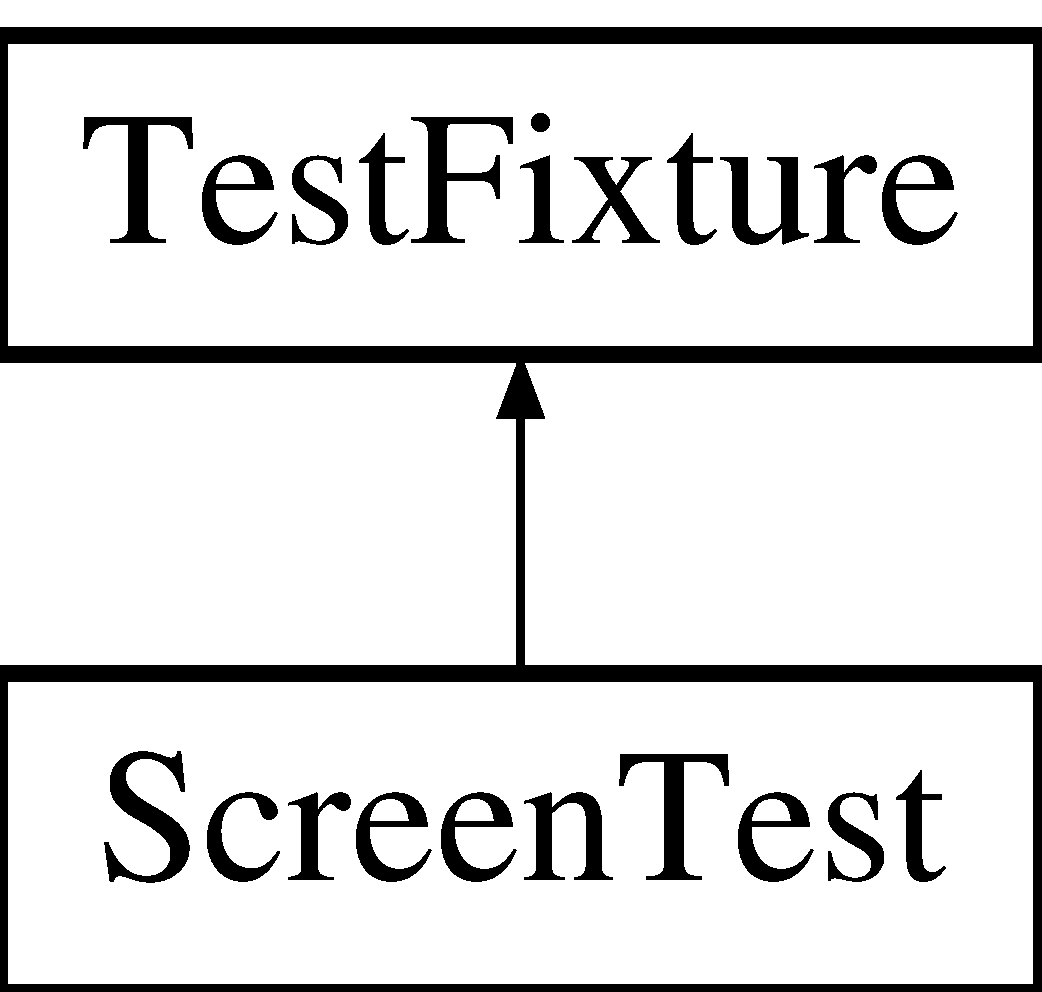
\includegraphics[height=2.000000cm]{classScreenTest}
\end{center}
\end{figure}
\subsection*{Public Member Functions}
\begin{DoxyCompactItemize}
\item 
void \hyperlink{classScreenTest_a7eadae1233e3a94cc10b1f9defb66882}{set\-Up} ()
\begin{DoxyCompactList}\small\item\em function to set up the variables \end{DoxyCompactList}\item 
void \hyperlink{classScreenTest_a779a3a2e83e9e169475e0d70049ceacb}{test\-Too\-Large} ()
\begin{DoxyCompactList}\small\item\em tests finding a large number \end{DoxyCompactList}\item 
void \hyperlink{classScreenTest_a3b09794a59af0142d36fade9aa311aa4}{test\-Too\-Small} ()
\begin{DoxyCompactList}\small\item\em tests finding a small number \end{DoxyCompactList}\item 
void \hyperlink{classScreenTest_ab62c1ff5c4f56cbb861e4a5540f43cc1}{test\-Negative} ()
\begin{DoxyCompactList}\small\item\em tests negative number \end{DoxyCompactList}\item 
void \hyperlink{classScreenTest_a4595a99a5ebbf7ee134cd6538ecace67}{test\-Created} ()
\begin{DoxyCompactList}\small\item\em tests if the screen exists \end{DoxyCompactList}\end{DoxyCompactItemize}


\subsection{Detailed Description}
class to test functionality of the \hyperlink{classScreen}{Screen} class 

\subsection{Member Function Documentation}
\hypertarget{classScreenTest_a7eadae1233e3a94cc10b1f9defb66882}{\index{Screen\-Test@{Screen\-Test}!set\-Up@{set\-Up}}
\index{set\-Up@{set\-Up}!ScreenTest@{Screen\-Test}}
\subsubsection[{set\-Up}]{\setlength{\rightskip}{0pt plus 5cm}void Screen\-Test\-::set\-Up (
\begin{DoxyParamCaption}
{}
\end{DoxyParamCaption}
)}}\label{classScreenTest_a7eadae1233e3a94cc10b1f9defb66882}


function to set up the variables 

Create some variables to test with. \hypertarget{classScreenTest_a4595a99a5ebbf7ee134cd6538ecace67}{\index{Screen\-Test@{Screen\-Test}!test\-Created@{test\-Created}}
\index{test\-Created@{test\-Created}!ScreenTest@{Screen\-Test}}
\subsubsection[{test\-Created}]{\setlength{\rightskip}{0pt plus 5cm}void Screen\-Test\-::test\-Created (
\begin{DoxyParamCaption}
{}
\end{DoxyParamCaption}
)}}\label{classScreenTest_a4595a99a5ebbf7ee134cd6538ecace67}


tests if the screen exists 

Tests for a large number. \hypertarget{classScreenTest_ab62c1ff5c4f56cbb861e4a5540f43cc1}{\index{Screen\-Test@{Screen\-Test}!test\-Negative@{test\-Negative}}
\index{test\-Negative@{test\-Negative}!ScreenTest@{Screen\-Test}}
\subsubsection[{test\-Negative}]{\setlength{\rightskip}{0pt plus 5cm}void Screen\-Test\-::test\-Negative (
\begin{DoxyParamCaption}
{}
\end{DoxyParamCaption}
)}}\label{classScreenTest_ab62c1ff5c4f56cbb861e4a5540f43cc1}


tests negative number 

Tests for a negative number. \hypertarget{classScreenTest_a779a3a2e83e9e169475e0d70049ceacb}{\index{Screen\-Test@{Screen\-Test}!test\-Too\-Large@{test\-Too\-Large}}
\index{test\-Too\-Large@{test\-Too\-Large}!ScreenTest@{Screen\-Test}}
\subsubsection[{test\-Too\-Large}]{\setlength{\rightskip}{0pt plus 5cm}void Screen\-Test\-::test\-Too\-Large (
\begin{DoxyParamCaption}
{}
\end{DoxyParamCaption}
)}}\label{classScreenTest_a779a3a2e83e9e169475e0d70049ceacb}


tests finding a large number 

Tests for a small number. \hypertarget{classScreenTest_a3b09794a59af0142d36fade9aa311aa4}{\index{Screen\-Test@{Screen\-Test}!test\-Too\-Small@{test\-Too\-Small}}
\index{test\-Too\-Small@{test\-Too\-Small}!ScreenTest@{Screen\-Test}}
\subsubsection[{test\-Too\-Small}]{\setlength{\rightskip}{0pt plus 5cm}void Screen\-Test\-::test\-Too\-Small (
\begin{DoxyParamCaption}
{}
\end{DoxyParamCaption}
)}}\label{classScreenTest_a3b09794a59af0142d36fade9aa311aa4}


tests finding a small number 

Tests for a sorted Array. 

The documentation for this class was generated from the following files\-:\begin{DoxyCompactItemize}
\item 
Screen/Screen\-Test.\-h\item 
Screen/Screen\-Test.\-cpp\end{DoxyCompactItemize}

\hypertarget{classSlotScreen}{\section{Slot\-Screen Class Reference}
\label{classSlotScreen}\index{Slot\-Screen@{Slot\-Screen}}
}


The \hyperlink{classSlotScreen}{Slot\-Screen} class represents a screen that displays an array of images.  




{\ttfamily \#include $<$Slot\-Screen.\-h$>$}

Inheritance diagram for Slot\-Screen\-:\begin{figure}[H]
\begin{center}
\leavevmode
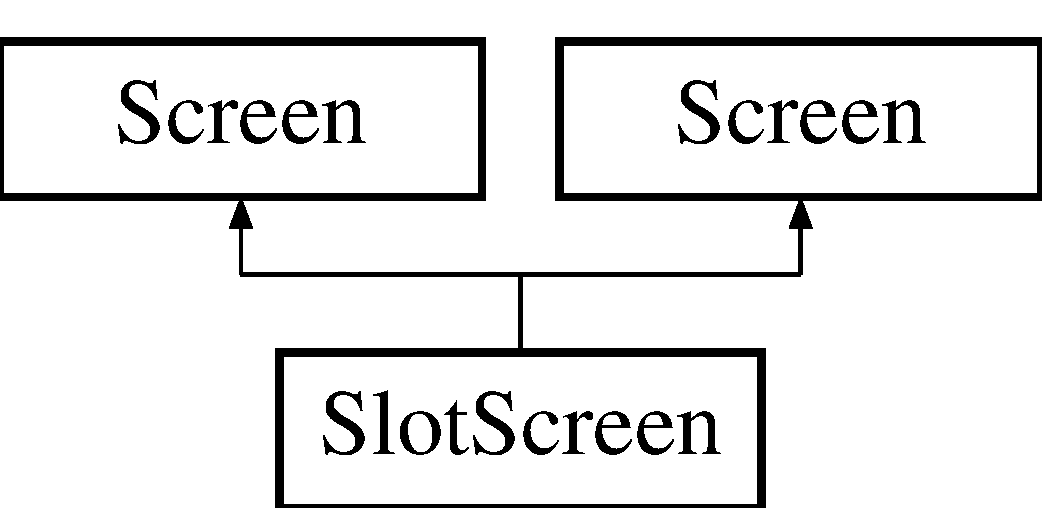
\includegraphics[height=2.000000cm]{classSlotScreen}
\end{center}
\end{figure}
\subsection*{Public Member Functions}
\begin{DoxyCompactItemize}
\item 
\hyperlink{classSlotScreen_a55b2a1537eb5cf4735f624e50946bc5a}{Slot\-Screen} (int h=13, int w=101, int slots=1)
\item 
\hypertarget{classSlotScreen_a1978a574c2835aeafd746ff3813c7253}{\hyperlink{classSlotScreen_a1978a574c2835aeafd746ff3813c7253}{$\sim$\-Slot\-Screen} ()}\label{classSlotScreen_a1978a574c2835aeafd746ff3813c7253}

\begin{DoxyCompactList}\small\item\em Destructor. \end{DoxyCompactList}\item 
\hyperlink{classSlotScreen_a55b2a1537eb5cf4735f624e50946bc5a}{Slot\-Screen} (int h=13, int w=101, int slots=1)
\item 
\hypertarget{classSlotScreen_a1978a574c2835aeafd746ff3813c7253}{\hyperlink{classSlotScreen_a1978a574c2835aeafd746ff3813c7253}{$\sim$\-Slot\-Screen} ()}\label{classSlotScreen_a1978a574c2835aeafd746ff3813c7253}

\begin{DoxyCompactList}\small\item\em Destructor. \end{DoxyCompactList}\end{DoxyCompactItemize}
\subsection*{Additional Inherited Members}


\subsection{Detailed Description}
The \hyperlink{classSlotScreen}{Slot\-Screen} class represents a screen that displays an array of images. 

\subsection{Constructor \& Destructor Documentation}
\hypertarget{classSlotScreen_a55b2a1537eb5cf4735f624e50946bc5a}{\index{Slot\-Screen@{Slot\-Screen}!Slot\-Screen@{Slot\-Screen}}
\index{Slot\-Screen@{Slot\-Screen}!SlotScreen@{Slot\-Screen}}
\subsubsection[{Slot\-Screen}]{\setlength{\rightskip}{0pt plus 5cm}Slot\-Screen\-::\-Slot\-Screen (
\begin{DoxyParamCaption}
\item[{int}]{h = {\ttfamily 13}, }
\item[{int}]{w = {\ttfamily 101}, }
\item[{int}]{slots = {\ttfamily 1}}
\end{DoxyParamCaption}
)}}\label{classSlotScreen_a55b2a1537eb5cf4735f624e50946bc5a}
Constructs an \hyperlink{classImage}{Image} object from the given dimensions 
\begin{DoxyParams}[1]{Parameters}
\mbox{\tt in}  & {\em h} & the height of the image, default to 13 \\
\hline
\mbox{\tt in}  & {\em w} & the width of the image, default to 101 \\
\hline
\mbox{\tt in}  & {\em slots} & the amount of images to be evenly spaced, default to 1 \\
\hline
\end{DoxyParams}
\hypertarget{classSlotScreen_a55b2a1537eb5cf4735f624e50946bc5a}{\index{Slot\-Screen@{Slot\-Screen}!Slot\-Screen@{Slot\-Screen}}
\index{Slot\-Screen@{Slot\-Screen}!SlotScreen@{Slot\-Screen}}
\subsubsection[{Slot\-Screen}]{\setlength{\rightskip}{0pt plus 5cm}Slot\-Screen\-::\-Slot\-Screen (
\begin{DoxyParamCaption}
\item[{int}]{h = {\ttfamily 13}, }
\item[{int}]{w = {\ttfamily 101}, }
\item[{int}]{slots = {\ttfamily 1}}
\end{DoxyParamCaption}
)}}\label{classSlotScreen_a55b2a1537eb5cf4735f624e50946bc5a}
Constructs an \hyperlink{classImage}{Image} object from the given dimensions 
\begin{DoxyParams}[1]{Parameters}
\mbox{\tt in}  & {\em h} & the height of the image, default to 13 \\
\hline
\mbox{\tt in}  & {\em w} & the width of the image, default to 101 \\
\hline
\mbox{\tt in}  & {\em slots} & the amount of images to be evenly spaced, default to 1 \\
\hline
\end{DoxyParams}


The documentation for this class was generated from the following files\-:\begin{DoxyCompactItemize}
\item 
Screen/Slot\-Screen.\-h\item 
Screen/Slot\-Screen.\-hh\item 
Screen/Slot\-Screen.\-cpp\end{DoxyCompactItemize}

\hypertarget{classSpell}{\section{Spell Class Reference}
\label{classSpell}\index{Spell@{Spell}}
}


Subclass of \hyperlink{classWeapon}{Weapon} to represent a spell in game.  




{\ttfamily \#include $<$My\-Weapons.\-h$>$}

Inheritance diagram for Spell\-:\begin{figure}[H]
\begin{center}
\leavevmode
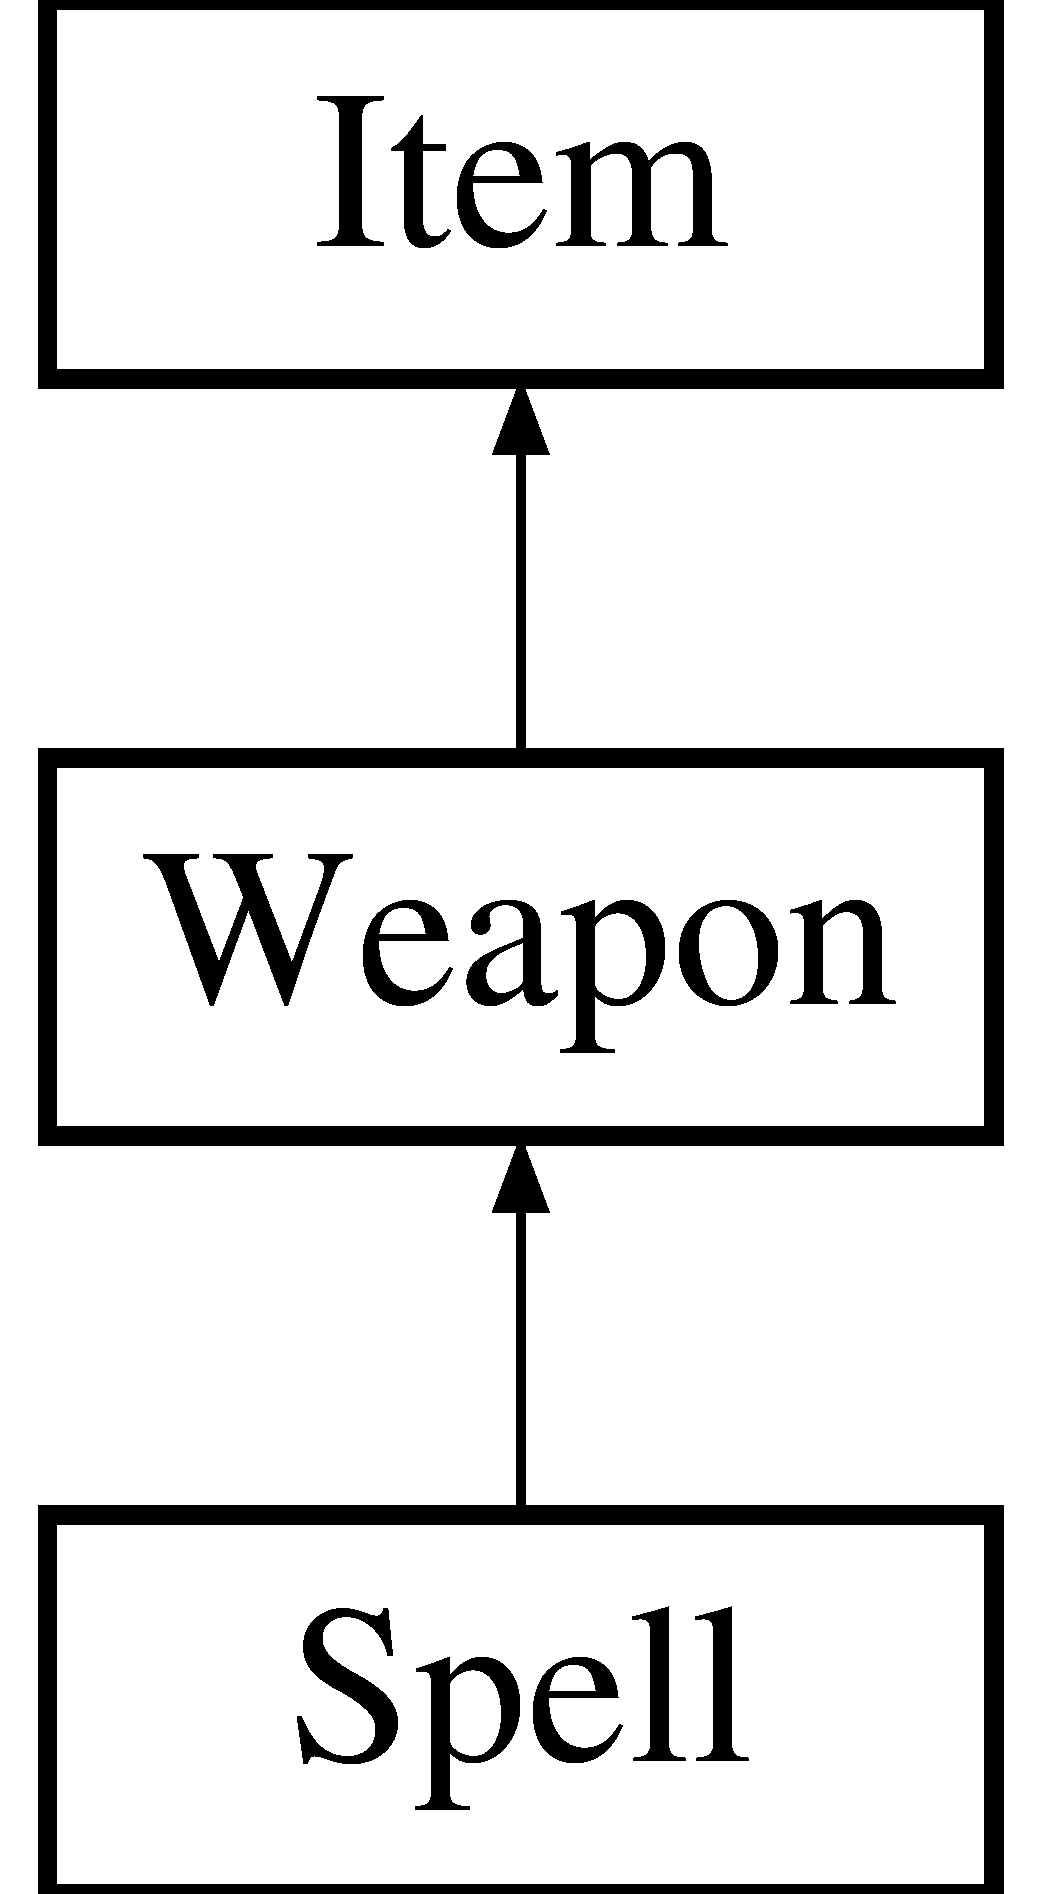
\includegraphics[height=3.000000cm]{classSpell}
\end{center}
\end{figure}
\subsection*{Public Member Functions}
\begin{DoxyCompactItemize}
\item 
\hyperlink{classSpell_a614361c1702859a162e1572030166cb0}{Spell} ()
\begin{DoxyCompactList}\small\item\em Constructor. \end{DoxyCompactList}\item 
bool \hyperlink{classSpell_a22680a625dce4f3a85421c4763930b57}{Use} (\hyperlink{classCharacter}{Character} $\ast$target)
\begin{DoxyCompactList}\small\item\em Use \hyperlink{classSpell}{Spell} Implementation. \end{DoxyCompactList}\end{DoxyCompactItemize}
\subsection*{Additional Inherited Members}


\subsection{Detailed Description}
Subclass of \hyperlink{classWeapon}{Weapon} to represent a spell in game. 

\subsection{Constructor \& Destructor Documentation}
\hypertarget{classSpell_a614361c1702859a162e1572030166cb0}{\index{Spell@{Spell}!Spell@{Spell}}
\index{Spell@{Spell}!Spell@{Spell}}
\subsubsection[{Spell}]{\setlength{\rightskip}{0pt plus 5cm}Spell\-::\-Spell (
\begin{DoxyParamCaption}
{}
\end{DoxyParamCaption}
)}}\label{classSpell_a614361c1702859a162e1572030166cb0}


Constructor. 

\hyperlink{classSpell}{Spell} Constructor. 

\subsection{Member Function Documentation}
\hypertarget{classSpell_a22680a625dce4f3a85421c4763930b57}{\index{Spell@{Spell}!Use@{Use}}
\index{Use@{Use}!Spell@{Spell}}
\subsubsection[{Use}]{\setlength{\rightskip}{0pt plus 5cm}bool Spell\-::\-Use (
\begin{DoxyParamCaption}
\item[{{\bf Character} $\ast$}]{target}
\end{DoxyParamCaption}
)\hspace{0.3cm}{\ttfamily [virtual]}}}\label{classSpell_a22680a625dce4f3a85421c4763930b57}


Use \hyperlink{classSpell}{Spell} Implementation. 

Defines what happens when the spell is used 
\begin{DoxyParams}[1]{Parameters}
\mbox{\tt in}  & {\em target} & The character that the spell is used on \\
\hline
\end{DoxyParams}
\begin{DoxyReturn}{Returns}
true if use was successfull 
\end{DoxyReturn}


Implements \hyperlink{classItem_abd3f52dd7fa25d497f2070e95d44ac03}{Item}.



The documentation for this class was generated from the following files\-:\begin{DoxyCompactItemize}
\item 
/home/rigt2720/\-Kodika/\-Item/\hyperlink{MyWeapons_8h}{My\-Weapons.\-h}\item 
/home/rigt2720/\-Kodika/\-Item/\hyperlink{MyWeapons_8cpp}{My\-Weapons.\-cpp}\end{DoxyCompactItemize}

\hypertarget{classSword}{\section{Sword Class Reference}
\label{classSword}\index{Sword@{Sword}}
}


Subclass of \hyperlink{classWeapon}{Weapon} to represent a sword in game.  




{\ttfamily \#include $<$My\-Weapons.\-h$>$}

Inheritance diagram for Sword\-:\begin{figure}[H]
\begin{center}
\leavevmode
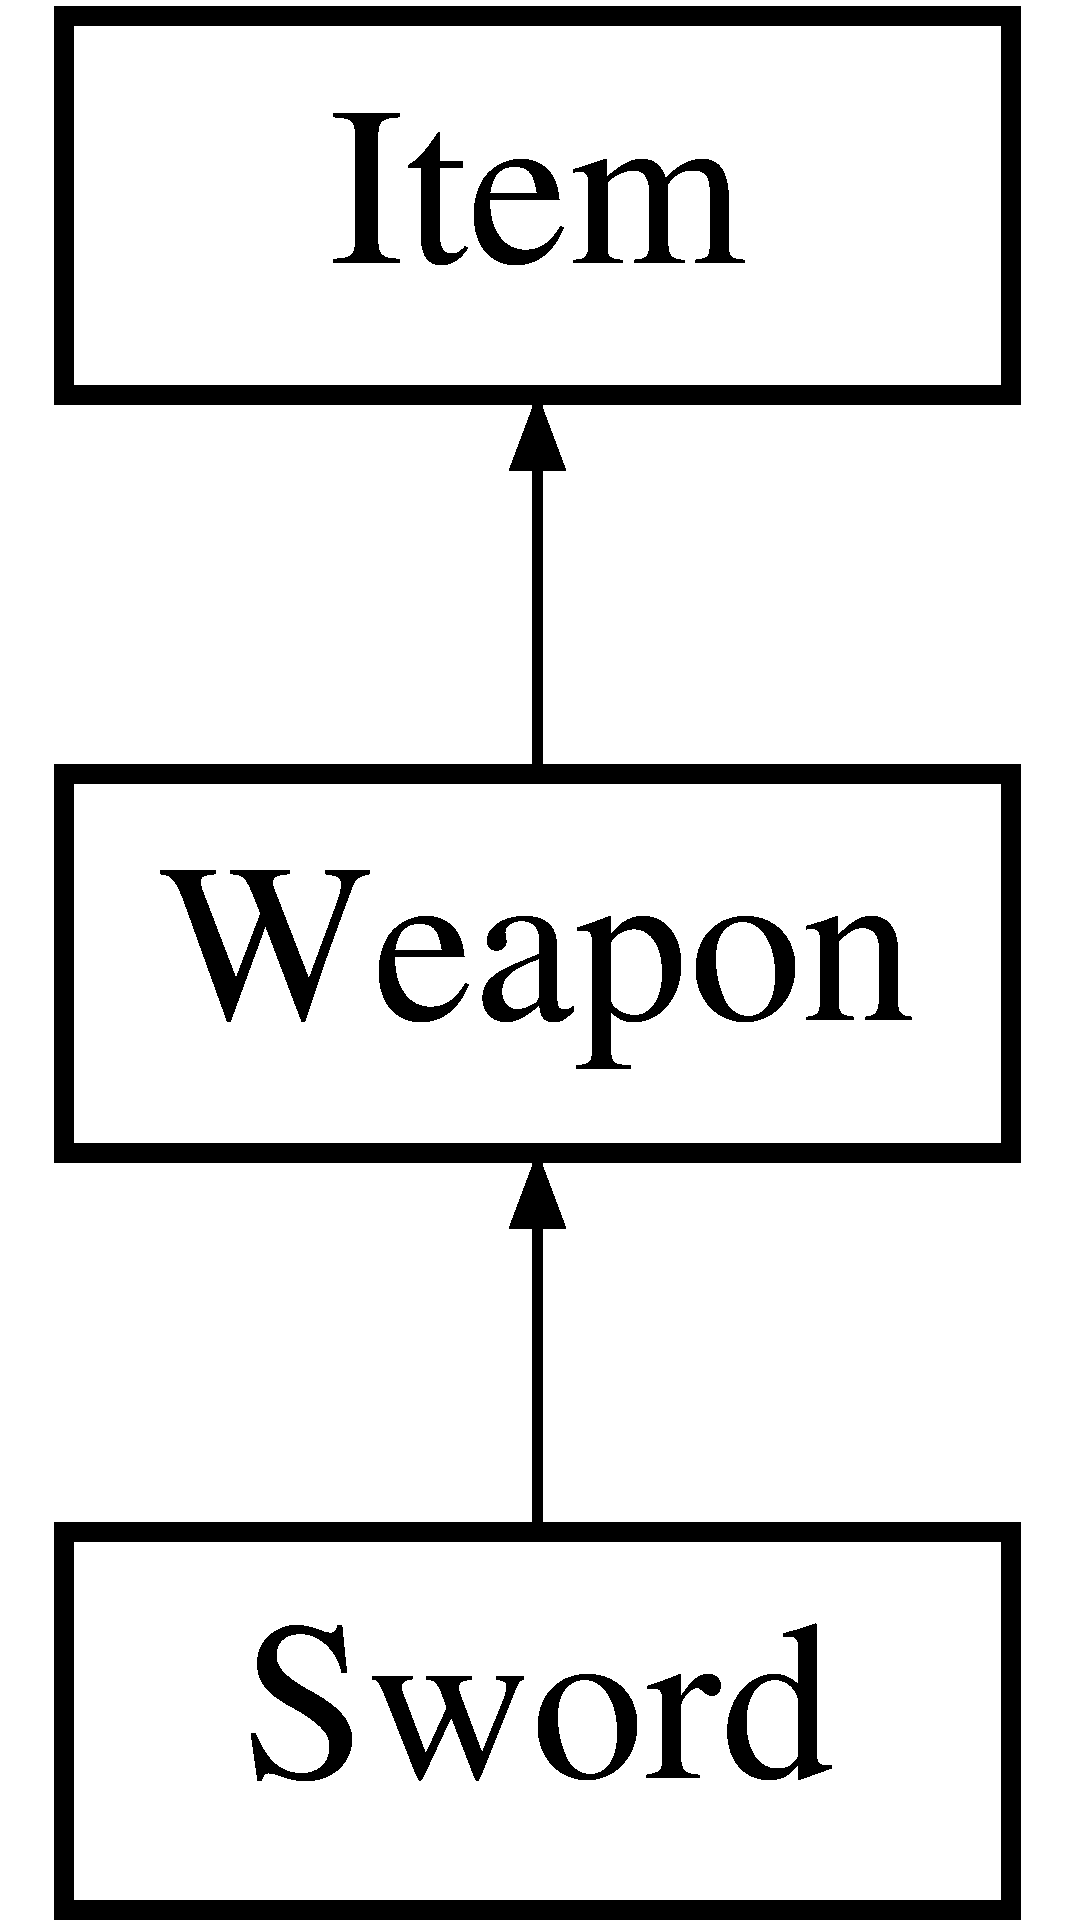
\includegraphics[height=3.000000cm]{classSword}
\end{center}
\end{figure}
\subsection*{Public Member Functions}
\begin{DoxyCompactItemize}
\item 
\hyperlink{classSword_af33284e40825ec8ddccd01fa5833be36}{Sword} ()
\begin{DoxyCompactList}\small\item\em Constructor. \end{DoxyCompactList}\item 
bool \hyperlink{classSword_ac9613c1b3c9a3b748c6e36b1285924b9}{use} (\hyperlink{classCharacter}{Character} $\ast$target)
\begin{DoxyCompactList}\small\item\em Use \hyperlink{classSword}{Sword} Implementation. \end{DoxyCompactList}\end{DoxyCompactItemize}
\subsection*{Additional Inherited Members}


\subsection{Detailed Description}
Subclass of \hyperlink{classWeapon}{Weapon} to represent a sword in game. 

\begin{DoxyAuthor}{Author}
Rylan Bueckert 
\end{DoxyAuthor}
\begin{DoxyDate}{Date}
Oct 25, 2017 
\end{DoxyDate}


\subsection{Constructor \& Destructor Documentation}
\hypertarget{classSword_af33284e40825ec8ddccd01fa5833be36}{\index{Sword@{Sword}!Sword@{Sword}}
\index{Sword@{Sword}!Sword@{Sword}}
\subsubsection[{Sword}]{\setlength{\rightskip}{0pt plus 5cm}Sword\-::\-Sword (
\begin{DoxyParamCaption}
{}
\end{DoxyParamCaption}
)}}\label{classSword_af33284e40825ec8ddccd01fa5833be36}


Constructor. 

\hyperlink{classSword}{Sword} Constructor. 

\subsection{Member Function Documentation}
\hypertarget{classSword_ac9613c1b3c9a3b748c6e36b1285924b9}{\index{Sword@{Sword}!use@{use}}
\index{use@{use}!Sword@{Sword}}
\subsubsection[{use}]{\setlength{\rightskip}{0pt plus 5cm}bool Sword\-::use (
\begin{DoxyParamCaption}
\item[{{\bf Character} $\ast$}]{target}
\end{DoxyParamCaption}
)\hspace{0.3cm}{\ttfamily [virtual]}}}\label{classSword_ac9613c1b3c9a3b748c6e36b1285924b9}


Use \hyperlink{classSword}{Sword} Implementation. 

Defines what happens when the sword is used 
\begin{DoxyParams}[1]{Parameters}
\mbox{\tt in}  & {\em target} & The character that the sword is used on \\
\hline
\end{DoxyParams}
\begin{DoxyReturn}{Returns}
true if use was successfull 
\end{DoxyReturn}


Implements \hyperlink{classItem_a790283e2fb63df00eb61a95bb9921051}{Item}.



The documentation for this class was generated from the following files\-:\begin{DoxyCompactItemize}
\item 
/home/rigt2720/\-Kodika/\-Item/\hyperlink{MyWeapons_8h}{My\-Weapons.\-h}\item 
/home/rigt2720/\-Kodika/\-Item/\hyperlink{MyWeapons_8cpp}{My\-Weapons.\-cpp}\end{DoxyCompactItemize}

\hypertarget{classTicTacToe}{\section{Tic\-Tac\-Toe Class Reference}
\label{classTicTacToe}\index{Tic\-Tac\-Toe@{Tic\-Tac\-Toe}}
}


This class contains the mini-\/game/puzzle Tic Tac Toe.  




{\ttfamily \#include $<$Tic\-Tac\-Toe.\-h$>$}

Inheritance diagram for Tic\-Tac\-Toe\-:\begin{figure}[H]
\begin{center}
\leavevmode
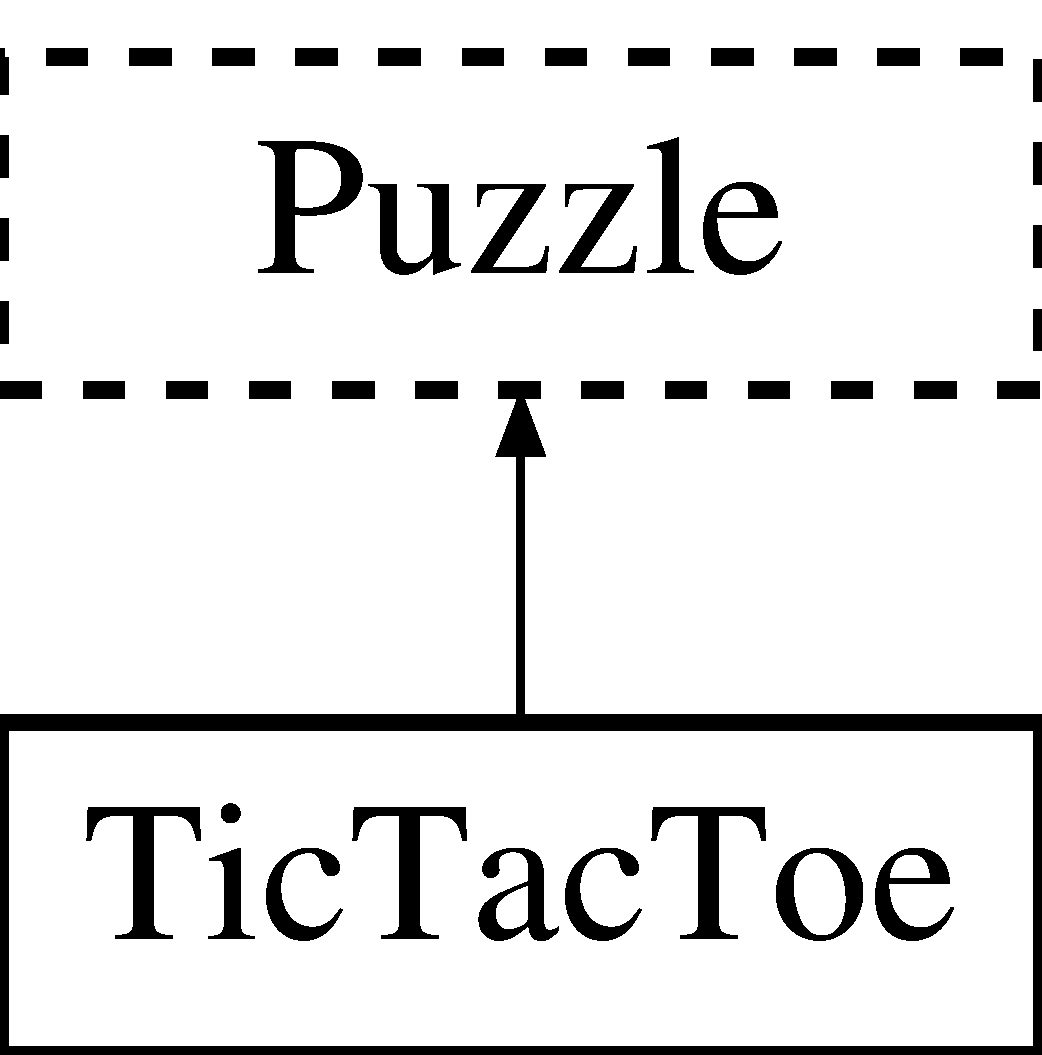
\includegraphics[height=2.000000cm]{classTicTacToe}
\end{center}
\end{figure}
\subsection*{Public Member Functions}
\begin{DoxyCompactItemize}
\item 
\hyperlink{classTicTacToe_a103fe9a5ae41b5ef756e20594a70cb7a}{Tic\-Tac\-Toe} ()
\begin{DoxyCompactList}\small\item\em Default constructor for \hyperlink{classTicTacToe}{Tic\-Tac\-Toe}, sets height to 3 and width to 3. \end{DoxyCompactList}\item 
virtual \hyperlink{classTicTacToe_a5e9c4ed3279034d5530cc7b94a3e10e5}{$\sim$\-Tic\-Tac\-Toe} ()
\begin{DoxyCompactList}\small\item\em Deconstructor. \end{DoxyCompactList}\item 
virtual void \hyperlink{classTicTacToe_acf4f00b2f56781f0c41a4d51cfe03268}{Run\-Game} (\hyperlink{classCharacter}{Character} $\ast$player)
\end{DoxyCompactItemize}
\subsection*{Private Member Functions}
\begin{DoxyCompactItemize}
\item 
bool \hyperlink{classTicTacToe_ab3e52a3c1bb9fefe08f4c4641f8a70f8}{Valid\-Move} (int input\-X, int input\-Y)
\item 
void \hyperlink{classTicTacToe_a5a03afaffde20d826472e7a8e27995e4}{Board\-Setup} ()
\begin{DoxyCompactList}\small\item\em Sets the board up for the beginning of the game, placing the grid. \end{DoxyCompactList}\item 
void \hyperlink{classTicTacToe_afb236f340525d12a81667a340440b210}{Move\-Piece} (int input\-X, int input\-Y, char user\-Piece)
\item 
void \hyperlink{classTicTacToe_a608d3101cab7340fcc2d0ea5061c37ea}{End\-Game\-Prompt} (int \&current\-Player, \hyperlink{classTicTacToeMenu}{Tic\-Tac\-Toe\-Menu} menu, \hyperlink{classCharacter}{Character} $\ast$player)
\item 
bool \hyperlink{classTicTacToe_afe8f0ecd818f9f6b8418b7e597ff56a7}{Win\-Check} ()
\begin{DoxyCompactList}\small\item\em Checks to see if there have been any 3 tokens in a row in the grid vector. \end{DoxyCompactList}\item 
bool \hyperlink{classTicTacToe_a8134bdddf731a29f61f42273e23f1abf}{Tie\-Game\-Check} (int \&current\-Player)
\item 
void \hyperlink{classTicTacToe_a457647024a551cb3d574d47a9ca85091}{Ai\-Move} (char Ai\-Piece)
\item 
bool \hyperlink{classTicTacToe_afce358eabb849ae0dbf55818a7bdc56b}{Horizontal\-Check} ()
\item 
bool \hyperlink{classTicTacToe_aff214a5737d06961a5f6a14cf97ed1fe}{Vertical\-Check} ()
\item 
bool \hyperlink{classTicTacToe_a3b96d4252e042b2e85bb0bc9a501bc0c}{Right\-Diagonal\-Check} ()
\item 
bool \hyperlink{classTicTacToe_ad65a6d8382d7a59c68a6778caea91d78}{Left\-Diagonal\-Check} ()
\item 
bool \hyperlink{classTicTacToe_a6c8bc2be4b6fc3f462905252c70b5183}{Is\-Input\-Valid} (char input\-X, int input\-Y)
\item 
bool \hyperlink{classTicTacToe_ab2b2442eaad32fe7bd57db13ca5db77f}{Is\-Int\-Input\-Valid} (int input)
\item 
void \hyperlink{classTicTacToe_a3c05c5ac2c16a02a6a3c3b2021fdde74}{Set\-Current\-Players\-Char} (int current\-Player)
\item 
void \hyperlink{classTicTacToe_a740fc2c6b0526442ead17835c473f93e}{Reset\-Game} (int \&current\-Player)
\item 
int \hyperlink{classTicTacToe_a40ab96fced3061640200f5e7b83e0415}{Convert\-Char\-Coordinate\-To\-Index} (char input)
\item 
bool \hyperlink{classTicTacToe_a7b1ba09a855c9a3f71e3e06b3e76a992}{Is\-Spot\-Filled} (int input\-X, int input\-Y)
\begin{DoxyCompactList}\small\item\em returns true if character is filled, false otherwise \end{DoxyCompactList}\item 
bool \hyperlink{classTicTacToe_a7bb5521e85c2a1d4c61ab405d03a62c5}{Is\-Board\-Full} ()
\begin{DoxyCompactList}\small\item\em Returns true if every space in the board has been filled with a character. \end{DoxyCompactList}\item 
void \hyperlink{classTicTacToe_a36b58f33246558d0b7b34412b641cff6}{Reset\-Game} ()
\begin{DoxyCompactList}\small\item\em Resets the game for another round in the event that the A\-I wins. \end{DoxyCompactList}\end{DoxyCompactItemize}
\subsection*{Private Attributes}
\begin{DoxyCompactItemize}
\item 
std\-::vector$<$ vector$<$ char $>$ $>$ \hyperlink{classTicTacToe_a56cd1b3760908be79d5fa311c2d17761}{game\-Board}
\begin{DoxyCompactList}\small\item\em Vector to store the contents of the gameboard. \end{DoxyCompactList}\item 
int \hyperlink{classTicTacToe_a0aab68285cb8b8f5ce6159ed5cfc8bbd}{board\-Size}
\begin{DoxyCompactList}\small\item\em Dimensions for the board. \end{DoxyCompactList}\item 
char \hyperlink{classTicTacToe_a914627e3dd8100c387e98c4a022b1457}{current\-Player\-Char}
\item 
\hyperlink{classScreen}{Screen} \hyperlink{classTicTacToe_a6749582a8480be3cbae920f8f2cca8ce}{Tic\-Tac\-Toe\-Screen}
\end{DoxyCompactItemize}
\subsection*{Additional Inherited Members}


\subsection{Detailed Description}
This class contains the mini-\/game/puzzle Tic Tac Toe. 

\subsection{Constructor \& Destructor Documentation}
\hypertarget{classTicTacToe_a103fe9a5ae41b5ef756e20594a70cb7a}{\index{Tic\-Tac\-Toe@{Tic\-Tac\-Toe}!Tic\-Tac\-Toe@{Tic\-Tac\-Toe}}
\index{Tic\-Tac\-Toe@{Tic\-Tac\-Toe}!TicTacToe@{Tic\-Tac\-Toe}}
\subsubsection[{Tic\-Tac\-Toe}]{\setlength{\rightskip}{0pt plus 5cm}Tic\-Tac\-Toe\-::\-Tic\-Tac\-Toe (
\begin{DoxyParamCaption}
{}
\end{DoxyParamCaption}
)}}\label{classTicTacToe_a103fe9a5ae41b5ef756e20594a70cb7a}


Default constructor for \hyperlink{classTicTacToe}{Tic\-Tac\-Toe}, sets height to 3 and width to 3. 

\begin{DoxyAuthor}{Author}
Tyler Siwy 
\end{DoxyAuthor}
\begin{DoxyDate}{Date}
Oct 20, 2017 
\end{DoxyDate}
Setting up the game vector \hypertarget{classTicTacToe_a5e9c4ed3279034d5530cc7b94a3e10e5}{\index{Tic\-Tac\-Toe@{Tic\-Tac\-Toe}!$\sim$\-Tic\-Tac\-Toe@{$\sim$\-Tic\-Tac\-Toe}}
\index{$\sim$\-Tic\-Tac\-Toe@{$\sim$\-Tic\-Tac\-Toe}!TicTacToe@{Tic\-Tac\-Toe}}
\subsubsection[{$\sim$\-Tic\-Tac\-Toe}]{\setlength{\rightskip}{0pt plus 5cm}Tic\-Tac\-Toe\-::$\sim$\-Tic\-Tac\-Toe (
\begin{DoxyParamCaption}
{}
\end{DoxyParamCaption}
)\hspace{0.3cm}{\ttfamily [virtual]}}}\label{classTicTacToe_a5e9c4ed3279034d5530cc7b94a3e10e5}


Deconstructor. 



\subsection{Member Function Documentation}
\hypertarget{classTicTacToe_a457647024a551cb3d574d47a9ca85091}{\index{Tic\-Tac\-Toe@{Tic\-Tac\-Toe}!Ai\-Move@{Ai\-Move}}
\index{Ai\-Move@{Ai\-Move}!TicTacToe@{Tic\-Tac\-Toe}}
\subsubsection[{Ai\-Move}]{\setlength{\rightskip}{0pt plus 5cm}void Tic\-Tac\-Toe\-::\-Ai\-Move (
\begin{DoxyParamCaption}
\item[{char}]{Ai\-Piece}
\end{DoxyParamCaption}
)\hspace{0.3cm}{\ttfamily [private]}}}\label{classTicTacToe_a457647024a551cb3d574d47a9ca85091}
Performs the selection for the npc opponent. 
\begin{DoxyParams}[1]{Parameters}
\mbox{\tt in}  & {\em Ai\-Piece,which} & char to insert into the board \\
\hline
\end{DoxyParams}
\hypertarget{classTicTacToe_a5a03afaffde20d826472e7a8e27995e4}{\index{Tic\-Tac\-Toe@{Tic\-Tac\-Toe}!Board\-Setup@{Board\-Setup}}
\index{Board\-Setup@{Board\-Setup}!TicTacToe@{Tic\-Tac\-Toe}}
\subsubsection[{Board\-Setup}]{\setlength{\rightskip}{0pt plus 5cm}void Tic\-Tac\-Toe\-::\-Board\-Setup (
\begin{DoxyParamCaption}
{}
\end{DoxyParamCaption}
)\hspace{0.3cm}{\ttfamily [private]}}}\label{classTicTacToe_a5a03afaffde20d826472e7a8e27995e4}


Sets the board up for the beginning of the game, placing the grid. 

Sets up the board with the ui for the \hyperlink{classTicTacToe}{Tic\-Tac\-Toe} game. If i is odd, fill the row with '-\/'

top\-Bound and left\-Bound should set the board centered inside the screen object.

top\-Bound and left\-Bound should set the board centered inside the screen object.

top\-Bound and left\-Bound should set the board centered inside the screen object. \hypertarget{classTicTacToe_a40ab96fced3061640200f5e7b83e0415}{\index{Tic\-Tac\-Toe@{Tic\-Tac\-Toe}!Convert\-Char\-Coordinate\-To\-Index@{Convert\-Char\-Coordinate\-To\-Index}}
\index{Convert\-Char\-Coordinate\-To\-Index@{Convert\-Char\-Coordinate\-To\-Index}!TicTacToe@{Tic\-Tac\-Toe}}
\subsubsection[{Convert\-Char\-Coordinate\-To\-Index}]{\setlength{\rightskip}{0pt plus 5cm}int Tic\-Tac\-Toe\-::\-Convert\-Char\-Coordinate\-To\-Index (
\begin{DoxyParamCaption}
\item[{char}]{input}
\end{DoxyParamCaption}
)\hspace{0.3cm}{\ttfamily [private]}}}\label{classTicTacToe_a40ab96fced3061640200f5e7b83e0415}
Takes a char from the input and assigns it an appropriate int 
\begin{DoxyParams}[1]{Parameters}
\mbox{\tt in}  & {\em a} & char to convert \\
\hline
\end{DoxyParams}
\hypertarget{classTicTacToe_a608d3101cab7340fcc2d0ea5061c37ea}{\index{Tic\-Tac\-Toe@{Tic\-Tac\-Toe}!End\-Game\-Prompt@{End\-Game\-Prompt}}
\index{End\-Game\-Prompt@{End\-Game\-Prompt}!TicTacToe@{Tic\-Tac\-Toe}}
\subsubsection[{End\-Game\-Prompt}]{\setlength{\rightskip}{0pt plus 5cm}void Tic\-Tac\-Toe\-::\-End\-Game\-Prompt (
\begin{DoxyParamCaption}
\item[{int \&}]{current\-Player, }
\item[{{\bf Tic\-Tac\-Toe\-Menu}}]{menu, }
\item[{{\bf Character} $\ast$}]{player}
\end{DoxyParamCaption}
)\hspace{0.3cm}{\ttfamily [private]}}}\label{classTicTacToe_a608d3101cab7340fcc2d0ea5061c37ea}
Prompts the player and handles the end of the game appropriately. 
\begin{DoxyParams}[1]{Parameters}
\mbox{\tt in}  & {\em current\-Player,assigned} & to be human for new game. \mbox{[}in\mbox{]} menu, the menu used to output stuffs \\
\hline
\mbox{\tt in}  & {\em player,a} & pointer to the player usd to modify stats \\
\hline
\end{DoxyParams}
If current\-Player is even, the A\-I has won, -\/1 player health, reset the game for another round until the player has won. \hypertarget{classTicTacToe_afce358eabb849ae0dbf55818a7bdc56b}{\index{Tic\-Tac\-Toe@{Tic\-Tac\-Toe}!Horizontal\-Check@{Horizontal\-Check}}
\index{Horizontal\-Check@{Horizontal\-Check}!TicTacToe@{Tic\-Tac\-Toe}}
\subsubsection[{Horizontal\-Check}]{\setlength{\rightskip}{0pt plus 5cm}bool Tic\-Tac\-Toe\-::\-Horizontal\-Check (
\begin{DoxyParamCaption}
{}
\end{DoxyParamCaption}
)\hspace{0.3cm}{\ttfamily [private]}}}\label{classTicTacToe_afce358eabb849ae0dbf55818a7bdc56b}
Checks the entire grid to see if there is 3 of a kind in a horizontal position, returns true if it finds 3 of a kind, false otherwise.

Checks the entire grid to see if there is 3 of a kind in the horizontal position, returns true if it finds 3 of a kind, false otherwise. \hypertarget{classTicTacToe_a7bb5521e85c2a1d4c61ab405d03a62c5}{\index{Tic\-Tac\-Toe@{Tic\-Tac\-Toe}!Is\-Board\-Full@{Is\-Board\-Full}}
\index{Is\-Board\-Full@{Is\-Board\-Full}!TicTacToe@{Tic\-Tac\-Toe}}
\subsubsection[{Is\-Board\-Full}]{\setlength{\rightskip}{0pt plus 5cm}bool Tic\-Tac\-Toe\-::\-Is\-Board\-Full (
\begin{DoxyParamCaption}
{}
\end{DoxyParamCaption}
)\hspace{0.3cm}{\ttfamily [private]}}}\label{classTicTacToe_a7bb5521e85c2a1d4c61ab405d03a62c5}


Returns true if every space in the board has been filled with a character. 

\hypertarget{classTicTacToe_a6c8bc2be4b6fc3f462905252c70b5183}{\index{Tic\-Tac\-Toe@{Tic\-Tac\-Toe}!Is\-Input\-Valid@{Is\-Input\-Valid}}
\index{Is\-Input\-Valid@{Is\-Input\-Valid}!TicTacToe@{Tic\-Tac\-Toe}}
\subsubsection[{Is\-Input\-Valid}]{\setlength{\rightskip}{0pt plus 5cm}bool Tic\-Tac\-Toe\-::\-Is\-Input\-Valid (
\begin{DoxyParamCaption}
\item[{char}]{input\-X, }
\item[{int}]{input\-Y}
\end{DoxyParamCaption}
)\hspace{0.3cm}{\ttfamily [private]}}}\label{classTicTacToe_a6c8bc2be4b6fc3f462905252c70b5183}
Makes sure the input is within the bounds of the game 
\begin{DoxyParams}[1]{Parameters}
\mbox{\tt in}  & {\em x-\/coordinate} & to check \\
\hline
\mbox{\tt in}  & {\em y-\/coordinate} & to check \\
\hline
\end{DoxyParams}
\hypertarget{classTicTacToe_ab2b2442eaad32fe7bd57db13ca5db77f}{\index{Tic\-Tac\-Toe@{Tic\-Tac\-Toe}!Is\-Int\-Input\-Valid@{Is\-Int\-Input\-Valid}}
\index{Is\-Int\-Input\-Valid@{Is\-Int\-Input\-Valid}!TicTacToe@{Tic\-Tac\-Toe}}
\subsubsection[{Is\-Int\-Input\-Valid}]{\setlength{\rightskip}{0pt plus 5cm}bool Tic\-Tac\-Toe\-::\-Is\-Int\-Input\-Valid (
\begin{DoxyParamCaption}
\item[{int}]{input}
\end{DoxyParamCaption}
)\hspace{0.3cm}{\ttfamily [private]}}}\label{classTicTacToe_ab2b2442eaad32fe7bd57db13ca5db77f}
Checks to see if the int is within the bounds of the game 
\begin{DoxyParams}[1]{Parameters}
\mbox{\tt in}  & {\em the} & value to check \\
\hline
\end{DoxyParams}
\hypertarget{classTicTacToe_a7b1ba09a855c9a3f71e3e06b3e76a992}{\index{Tic\-Tac\-Toe@{Tic\-Tac\-Toe}!Is\-Spot\-Filled@{Is\-Spot\-Filled}}
\index{Is\-Spot\-Filled@{Is\-Spot\-Filled}!TicTacToe@{Tic\-Tac\-Toe}}
\subsubsection[{Is\-Spot\-Filled}]{\setlength{\rightskip}{0pt plus 5cm}bool Tic\-Tac\-Toe\-::\-Is\-Spot\-Filled (
\begin{DoxyParamCaption}
\item[{int}]{input\-X, }
\item[{int}]{input\-Y}
\end{DoxyParamCaption}
)\hspace{0.3cm}{\ttfamily [private]}}}\label{classTicTacToe_a7b1ba09a855c9a3f71e3e06b3e76a992}


returns true if character is filled, false otherwise 

\hypertarget{classTicTacToe_ad65a6d8382d7a59c68a6778caea91d78}{\index{Tic\-Tac\-Toe@{Tic\-Tac\-Toe}!Left\-Diagonal\-Check@{Left\-Diagonal\-Check}}
\index{Left\-Diagonal\-Check@{Left\-Diagonal\-Check}!TicTacToe@{Tic\-Tac\-Toe}}
\subsubsection[{Left\-Diagonal\-Check}]{\setlength{\rightskip}{0pt plus 5cm}bool Tic\-Tac\-Toe\-::\-Left\-Diagonal\-Check (
\begin{DoxyParamCaption}
{}
\end{DoxyParamCaption}
)\hspace{0.3cm}{\ttfamily [private]}}}\label{classTicTacToe_ad65a6d8382d7a59c68a6778caea91d78}
Checks the entire grid to see if there is 3 of a kind in a left diagonal position, returns true if it finds 3 of a kind, false otherwise.

Checks the entire grid to see if there is 3 of a kind in the left diagonal position, returns true if it finds 3 of a kind, false otherwise. \hypertarget{classTicTacToe_afb236f340525d12a81667a340440b210}{\index{Tic\-Tac\-Toe@{Tic\-Tac\-Toe}!Move\-Piece@{Move\-Piece}}
\index{Move\-Piece@{Move\-Piece}!TicTacToe@{Tic\-Tac\-Toe}}
\subsubsection[{Move\-Piece}]{\setlength{\rightskip}{0pt plus 5cm}void Tic\-Tac\-Toe\-::\-Move\-Piece (
\begin{DoxyParamCaption}
\item[{int}]{input\-X, }
\item[{int}]{input\-Y, }
\item[{char}]{user\-Piece}
\end{DoxyParamCaption}
)\hspace{0.3cm}{\ttfamily [private]}}}\label{classTicTacToe_afb236f340525d12a81667a340440b210}
Displays the screen containing the gameboard 
\begin{DoxyParams}[1]{Parameters}
\mbox{\tt in}  & {\em input\-X,the} & X-\/coordinate of the selection. \\
\hline
\mbox{\tt in}  & {\em input\-Y,the} & Y-\/coordinate of the selection. \\
\hline
\end{DoxyParams}
\hypertarget{classTicTacToe_a740fc2c6b0526442ead17835c473f93e}{\index{Tic\-Tac\-Toe@{Tic\-Tac\-Toe}!Reset\-Game@{Reset\-Game}}
\index{Reset\-Game@{Reset\-Game}!TicTacToe@{Tic\-Tac\-Toe}}
\subsubsection[{Reset\-Game}]{\setlength{\rightskip}{0pt plus 5cm}void Tic\-Tac\-Toe\-::\-Reset\-Game (
\begin{DoxyParamCaption}
\item[{int \&}]{current\-Player}
\end{DoxyParamCaption}
)\hspace{0.3cm}{\ttfamily [private]}}}\label{classTicTacToe_a740fc2c6b0526442ead17835c473f93e}
Resets the game to the starting state 
\begin{DoxyParams}[1]{Parameters}
\mbox{\tt in}  & {\em an} & int to show whos turn it is \\
\hline
\end{DoxyParams}
\hypertarget{classTicTacToe_a36b58f33246558d0b7b34412b641cff6}{\index{Tic\-Tac\-Toe@{Tic\-Tac\-Toe}!Reset\-Game@{Reset\-Game}}
\index{Reset\-Game@{Reset\-Game}!TicTacToe@{Tic\-Tac\-Toe}}
\subsubsection[{Reset\-Game}]{\setlength{\rightskip}{0pt plus 5cm}void Tic\-Tac\-Toe\-::\-Reset\-Game (
\begin{DoxyParamCaption}
{}
\end{DoxyParamCaption}
)\hspace{0.3cm}{\ttfamily [private]}}}\label{classTicTacToe_a36b58f33246558d0b7b34412b641cff6}


Resets the game for another round in the event that the A\-I wins. 

\hypertarget{classTicTacToe_a3b96d4252e042b2e85bb0bc9a501bc0c}{\index{Tic\-Tac\-Toe@{Tic\-Tac\-Toe}!Right\-Diagonal\-Check@{Right\-Diagonal\-Check}}
\index{Right\-Diagonal\-Check@{Right\-Diagonal\-Check}!TicTacToe@{Tic\-Tac\-Toe}}
\subsubsection[{Right\-Diagonal\-Check}]{\setlength{\rightskip}{0pt plus 5cm}bool Tic\-Tac\-Toe\-::\-Right\-Diagonal\-Check (
\begin{DoxyParamCaption}
{}
\end{DoxyParamCaption}
)\hspace{0.3cm}{\ttfamily [private]}}}\label{classTicTacToe_a3b96d4252e042b2e85bb0bc9a501bc0c}
Checks the entire grid to see if there's 3 of a kind in a right diagonal position, returns true if it finds 3 of a kind, false otherwise.

Checks the entire grid to see if there is 3 of a kind in the right diagonal position, returns true if it finds 3 of a kind, false otherwise. \hypertarget{classTicTacToe_acf4f00b2f56781f0c41a4d51cfe03268}{\index{Tic\-Tac\-Toe@{Tic\-Tac\-Toe}!Run\-Game@{Run\-Game}}
\index{Run\-Game@{Run\-Game}!TicTacToe@{Tic\-Tac\-Toe}}
\subsubsection[{Run\-Game}]{\setlength{\rightskip}{0pt plus 5cm}void Tic\-Tac\-Toe\-::\-Run\-Game (
\begin{DoxyParamCaption}
\item[{{\bf Character} $\ast$}]{player}
\end{DoxyParamCaption}
)\hspace{0.3cm}{\ttfamily [virtual]}}}\label{classTicTacToe_acf4f00b2f56781f0c41a4d51cfe03268}
Method to run the game, serves as a 'main' for the mini-\/game, calling functions from private until the player has won. current\-Player keeps track of whos turn it is, if it's odd, it is the user, if it is even, it is the A\-I's turn.

X is taken as a,b, or c, Y is taken in as an integer. 

Implements \hyperlink{classPuzzle_a134875b96b18d9963d2b018fd14e7ab9}{Puzzle}.

\hypertarget{classTicTacToe_a3c05c5ac2c16a02a6a3c3b2021fdde74}{\index{Tic\-Tac\-Toe@{Tic\-Tac\-Toe}!Set\-Current\-Players\-Char@{Set\-Current\-Players\-Char}}
\index{Set\-Current\-Players\-Char@{Set\-Current\-Players\-Char}!TicTacToe@{Tic\-Tac\-Toe}}
\subsubsection[{Set\-Current\-Players\-Char}]{\setlength{\rightskip}{0pt plus 5cm}void Tic\-Tac\-Toe\-::\-Set\-Current\-Players\-Char (
\begin{DoxyParamCaption}
\item[{int}]{current\-Player}
\end{DoxyParamCaption}
)\hspace{0.3cm}{\ttfamily [private]}}}\label{classTicTacToe_a3c05c5ac2c16a02a6a3c3b2021fdde74}
Checks who's turn it is and sets Current\-Player\-Char to their correct char. \hypertarget{classTicTacToe_a8134bdddf731a29f61f42273e23f1abf}{\index{Tic\-Tac\-Toe@{Tic\-Tac\-Toe}!Tie\-Game\-Check@{Tie\-Game\-Check}}
\index{Tie\-Game\-Check@{Tie\-Game\-Check}!TicTacToe@{Tic\-Tac\-Toe}}
\subsubsection[{Tie\-Game\-Check}]{\setlength{\rightskip}{0pt plus 5cm}bool Tic\-Tac\-Toe\-::\-Tie\-Game\-Check (
\begin{DoxyParamCaption}
\item[{int \&}]{current\-Player}
\end{DoxyParamCaption}
)\hspace{0.3cm}{\ttfamily [private]}}}\label{classTicTacToe_a8134bdddf731a29f61f42273e23f1abf}
Checks if there is a tie, returns true if yes. 
\begin{DoxyParams}[1]{Parameters}
\mbox{\tt in}  & {\em current\-Player,a} & reference to which players turn it is \\
\hline
\end{DoxyParams}
\hypertarget{classTicTacToe_ab3e52a3c1bb9fefe08f4c4641f8a70f8}{\index{Tic\-Tac\-Toe@{Tic\-Tac\-Toe}!Valid\-Move@{Valid\-Move}}
\index{Valid\-Move@{Valid\-Move}!TicTacToe@{Tic\-Tac\-Toe}}
\subsubsection[{Valid\-Move}]{\setlength{\rightskip}{0pt plus 5cm}bool Tic\-Tac\-Toe\-::\-Valid\-Move (
\begin{DoxyParamCaption}
\item[{int}]{input\-X, }
\item[{int}]{input\-Y}
\end{DoxyParamCaption}
)\hspace{0.3cm}{\ttfamily [private]}}}\label{classTicTacToe_ab3e52a3c1bb9fefe08f4c4641f8a70f8}
Checks the semantics of the user choice to make sure they aren't doing something that would break the game with their input. 
\begin{DoxyParams}[1]{Parameters}
\mbox{\tt in}  & {\em input\-X,the} & X-\/coordinate of the selection. \\
\hline
\mbox{\tt in}  & {\em input\-Y,the} & Y-\/coordinate of the selection. \\
\hline
\end{DoxyParams}
\hypertarget{classTicTacToe_aff214a5737d06961a5f6a14cf97ed1fe}{\index{Tic\-Tac\-Toe@{Tic\-Tac\-Toe}!Vertical\-Check@{Vertical\-Check}}
\index{Vertical\-Check@{Vertical\-Check}!TicTacToe@{Tic\-Tac\-Toe}}
\subsubsection[{Vertical\-Check}]{\setlength{\rightskip}{0pt plus 5cm}bool Tic\-Tac\-Toe\-::\-Vertical\-Check (
\begin{DoxyParamCaption}
{}
\end{DoxyParamCaption}
)\hspace{0.3cm}{\ttfamily [private]}}}\label{classTicTacToe_aff214a5737d06961a5f6a14cf97ed1fe}
Checks the entire grid to see if there is 3 of a kind in a vertical position, returns true if it finds 3 of a kind, false otherwise.

Checks the entire grid to see if there is 3 of a kind in the vertical position, returns true if it finds 3 of a kind, false otherwise. \hypertarget{classTicTacToe_afe8f0ecd818f9f6b8418b7e597ff56a7}{\index{Tic\-Tac\-Toe@{Tic\-Tac\-Toe}!Win\-Check@{Win\-Check}}
\index{Win\-Check@{Win\-Check}!TicTacToe@{Tic\-Tac\-Toe}}
\subsubsection[{Win\-Check}]{\setlength{\rightskip}{0pt plus 5cm}bool Tic\-Tac\-Toe\-::\-Win\-Check (
\begin{DoxyParamCaption}
{}
\end{DoxyParamCaption}
)\hspace{0.3cm}{\ttfamily [private]}}}\label{classTicTacToe_afe8f0ecd818f9f6b8418b7e597ff56a7}


Checks to see if there have been any 3 tokens in a row in the grid vector. 



\subsection{Member Data Documentation}
\hypertarget{classTicTacToe_a0aab68285cb8b8f5ce6159ed5cfc8bbd}{\index{Tic\-Tac\-Toe@{Tic\-Tac\-Toe}!board\-Size@{board\-Size}}
\index{board\-Size@{board\-Size}!TicTacToe@{Tic\-Tac\-Toe}}
\subsubsection[{board\-Size}]{\setlength{\rightskip}{0pt plus 5cm}int Tic\-Tac\-Toe\-::board\-Size\hspace{0.3cm}{\ttfamily [private]}}}\label{classTicTacToe_a0aab68285cb8b8f5ce6159ed5cfc8bbd}


Dimensions for the board. 

\hypertarget{classTicTacToe_a914627e3dd8100c387e98c4a022b1457}{\index{Tic\-Tac\-Toe@{Tic\-Tac\-Toe}!current\-Player\-Char@{current\-Player\-Char}}
\index{current\-Player\-Char@{current\-Player\-Char}!TicTacToe@{Tic\-Tac\-Toe}}
\subsubsection[{current\-Player\-Char}]{\setlength{\rightskip}{0pt plus 5cm}char Tic\-Tac\-Toe\-::current\-Player\-Char\hspace{0.3cm}{\ttfamily [private]}}}\label{classTicTacToe_a914627e3dd8100c387e98c4a022b1457}
\hypertarget{classTicTacToe_a56cd1b3760908be79d5fa311c2d17761}{\index{Tic\-Tac\-Toe@{Tic\-Tac\-Toe}!game\-Board@{game\-Board}}
\index{game\-Board@{game\-Board}!TicTacToe@{Tic\-Tac\-Toe}}
\subsubsection[{game\-Board}]{\setlength{\rightskip}{0pt plus 5cm}std\-::vector$<$ vector $<$ char $>$ $>$ Tic\-Tac\-Toe\-::game\-Board\hspace{0.3cm}{\ttfamily [private]}}}\label{classTicTacToe_a56cd1b3760908be79d5fa311c2d17761}


Vector to store the contents of the gameboard. 

\hypertarget{classTicTacToe_a6749582a8480be3cbae920f8f2cca8ce}{\index{Tic\-Tac\-Toe@{Tic\-Tac\-Toe}!Tic\-Tac\-Toe\-Screen@{Tic\-Tac\-Toe\-Screen}}
\index{Tic\-Tac\-Toe\-Screen@{Tic\-Tac\-Toe\-Screen}!TicTacToe@{Tic\-Tac\-Toe}}
\subsubsection[{Tic\-Tac\-Toe\-Screen}]{\setlength{\rightskip}{0pt plus 5cm}{\bf Screen} Tic\-Tac\-Toe\-::\-Tic\-Tac\-Toe\-Screen\hspace{0.3cm}{\ttfamily [private]}}}\label{classTicTacToe_a6749582a8480be3cbae920f8f2cca8ce}
Tic\-Tac\-Toe\-Screen stores and outputs the contents of the game to the terminal 

The documentation for this class was generated from the following files\-:\begin{DoxyCompactItemize}
\item 
/home/rigt2720/\-Kodika/\-Puzzles/\hyperlink{TicTacToe_8h}{Tic\-Tac\-Toe.\-h}\item 
/home/rigt2720/\-Kodika/\-Puzzles/\hyperlink{TicTacToe_8cpp}{Tic\-Tac\-Toe.\-cpp}\end{DoxyCompactItemize}

\hypertarget{classTicTacToeMenu}{\section{Tic\-Tac\-Toe\-Menu Class Reference}
\label{classTicTacToeMenu}\index{Tic\-Tac\-Toe\-Menu@{Tic\-Tac\-Toe\-Menu}}
}


This is the menu class for the Tic Tac Toe minigame.  




{\ttfamily \#include $<$Tic\-Tac\-Toe\-Menu.\-h$>$}

Inheritance diagram for Tic\-Tac\-Toe\-Menu\-:\begin{figure}[H]
\begin{center}
\leavevmode
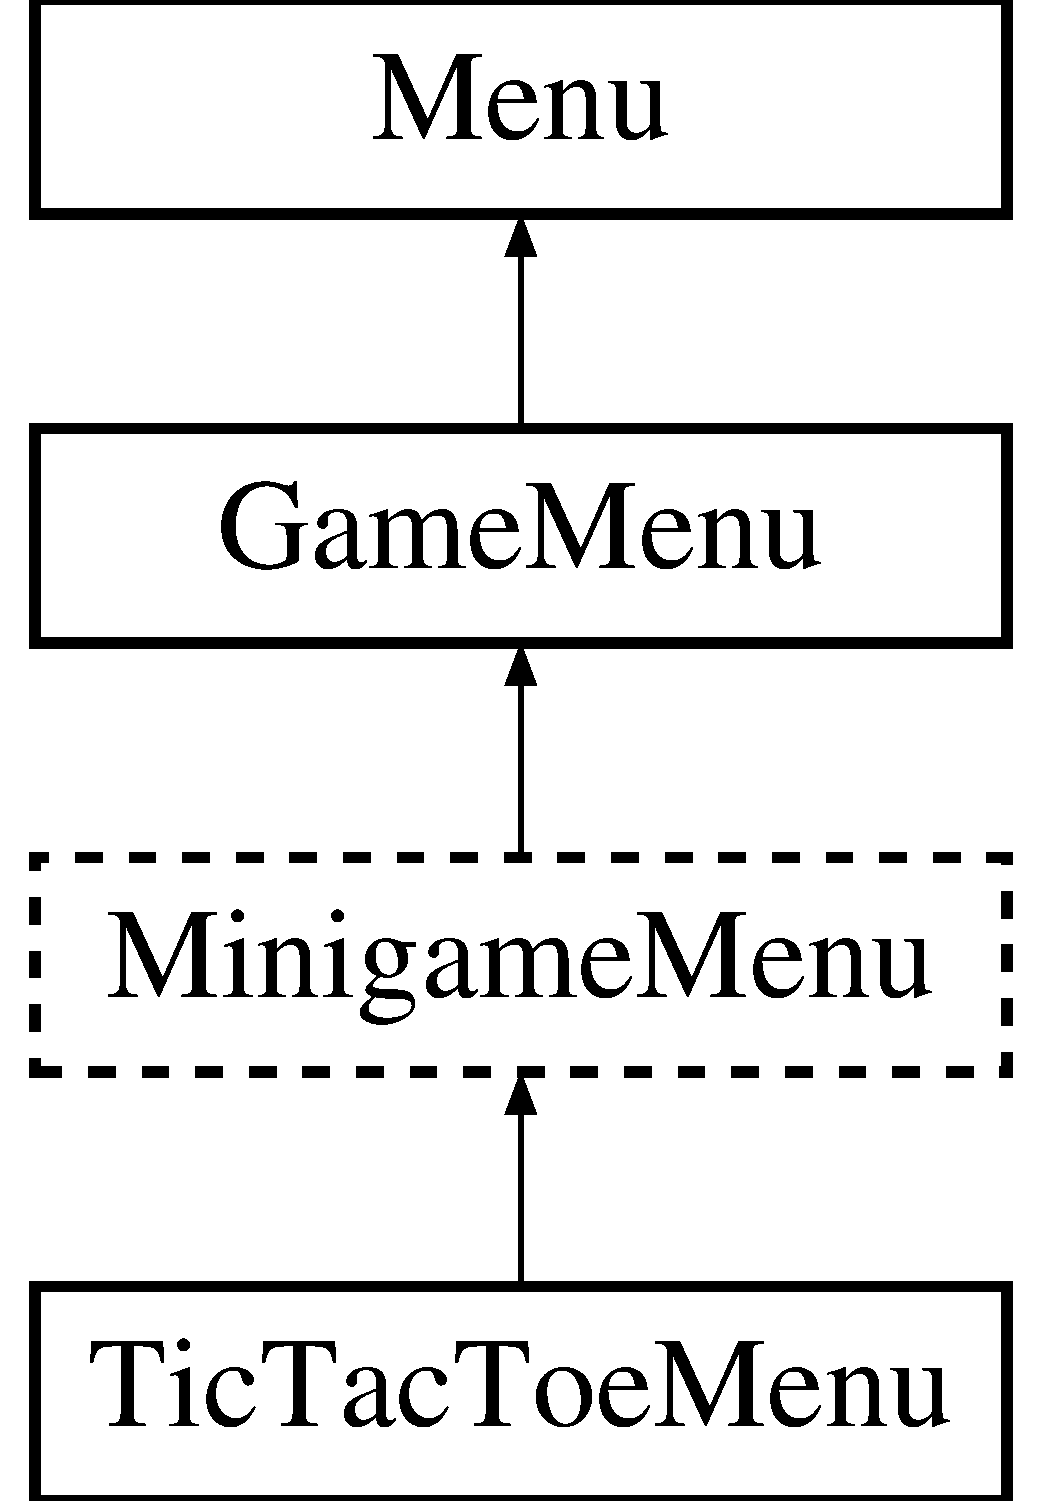
\includegraphics[height=4.000000cm]{classTicTacToeMenu}
\end{center}
\end{figure}
\subsection*{Public Member Functions}
\begin{DoxyCompactItemize}
\item 
\hypertarget{classTicTacToeMenu_a15e92bc5e44266bbc23bbce421186dad}{\hyperlink{classTicTacToeMenu_a15e92bc5e44266bbc23bbce421186dad}{Tic\-Tac\-Toe\-Menu} ()}\label{classTicTacToeMenu_a15e92bc5e44266bbc23bbce421186dad}

\begin{DoxyCompactList}\small\item\em This is the default constructor. \end{DoxyCompactList}\item 
\hypertarget{classTicTacToeMenu_a429d4d036694b8d96b08896f50d5f19b}{virtual \hyperlink{classTicTacToeMenu_a429d4d036694b8d96b08896f50d5f19b}{$\sim$\-Tic\-Tac\-Toe\-Menu} ()}\label{classTicTacToeMenu_a429d4d036694b8d96b08896f50d5f19b}

\begin{DoxyCompactList}\small\item\em This is the virtual destructor. \end{DoxyCompactList}\item 
virtual void \hyperlink{classTicTacToeMenu_a15f91b593ac1b58fc8b1b5267c9141d3}{Set\-Options} (map$<$ int, string $>$ options\-List, int row, int col)
\item 
virtual void \hyperlink{classTicTacToeMenu_a11191814019309260bb4270c03891e5e}{Handle\-Input} (istream \&is)
\end{DoxyCompactItemize}
\subsection*{Additional Inherited Members}


\subsection{Detailed Description}
This is the menu class for the Tic Tac Toe minigame. 

\subsection{Member Function Documentation}
\hypertarget{classTicTacToeMenu_a11191814019309260bb4270c03891e5e}{\index{Tic\-Tac\-Toe\-Menu@{Tic\-Tac\-Toe\-Menu}!Handle\-Input@{Handle\-Input}}
\index{Handle\-Input@{Handle\-Input}!TicTacToeMenu@{Tic\-Tac\-Toe\-Menu}}
\subsubsection[{Handle\-Input}]{\setlength{\rightskip}{0pt plus 5cm}void Tic\-Tac\-Toe\-Menu\-::\-Handle\-Input (
\begin{DoxyParamCaption}
\item[{istream \&}]{is}
\end{DoxyParamCaption}
)\hspace{0.3cm}{\ttfamily [virtual]}}}\label{classTicTacToeMenu_a11191814019309260bb4270c03891e5e}
This function handles the input for the menu options. 
\begin{DoxyParams}[1]{Parameters}
\mbox{\tt in,out}  & {\em is} & The in-\/stream operator to read the input. \\
\hline
\end{DoxyParams}


Implements \hyperlink{classMinigameMenu_a3f854c4eefb0f3110cd085b3cfe56460}{Minigame\-Menu}.

\hypertarget{classTicTacToeMenu_a15f91b593ac1b58fc8b1b5267c9141d3}{\index{Tic\-Tac\-Toe\-Menu@{Tic\-Tac\-Toe\-Menu}!Set\-Options@{Set\-Options}}
\index{Set\-Options@{Set\-Options}!TicTacToeMenu@{Tic\-Tac\-Toe\-Menu}}
\subsubsection[{Set\-Options}]{\setlength{\rightskip}{0pt plus 5cm}void Tic\-Tac\-Toe\-Menu\-::\-Set\-Options (
\begin{DoxyParamCaption}
\item[{map$<$ int, string $>$}]{options\-List, }
\item[{int}]{row, }
\item[{int}]{col}
\end{DoxyParamCaption}
)\hspace{0.3cm}{\ttfamily [virtual]}}}\label{classTicTacToeMenu_a15f91b593ac1b58fc8b1b5267c9141d3}
This function sets the specific options for the \hyperlink{classMenu}{Menu} type. 
\begin{DoxyParams}[1]{Parameters}
\mbox{\tt in}  & {\em Options\-List} & A map of all the options for the current menu. Each option has a unique key to make input easier. \\
\hline
\mbox{\tt in}  & {\em type} & This denotes the type of menu to display. \\
\hline
\end{DoxyParams}


The documentation for this class was generated from the following files\-:\begin{DoxyCompactItemize}
\item 
Menu/Tic\-Tac\-Toe\-Menu.\-h\item 
Menu/Tic\-Tac\-Toe\-Menu.\-cpp\end{DoxyCompactItemize}

\hypertarget{classTradeMenu}{\section{Trade\-Menu Class Reference}
\label{classTradeMenu}\index{Trade\-Menu@{Trade\-Menu}}
}


This is the menu displayed when the player character is trading.  




{\ttfamily \#include $<$Trade\-Menu.\-h$>$}

Inheritance diagram for Trade\-Menu\-:\begin{figure}[H]
\begin{center}
\leavevmode
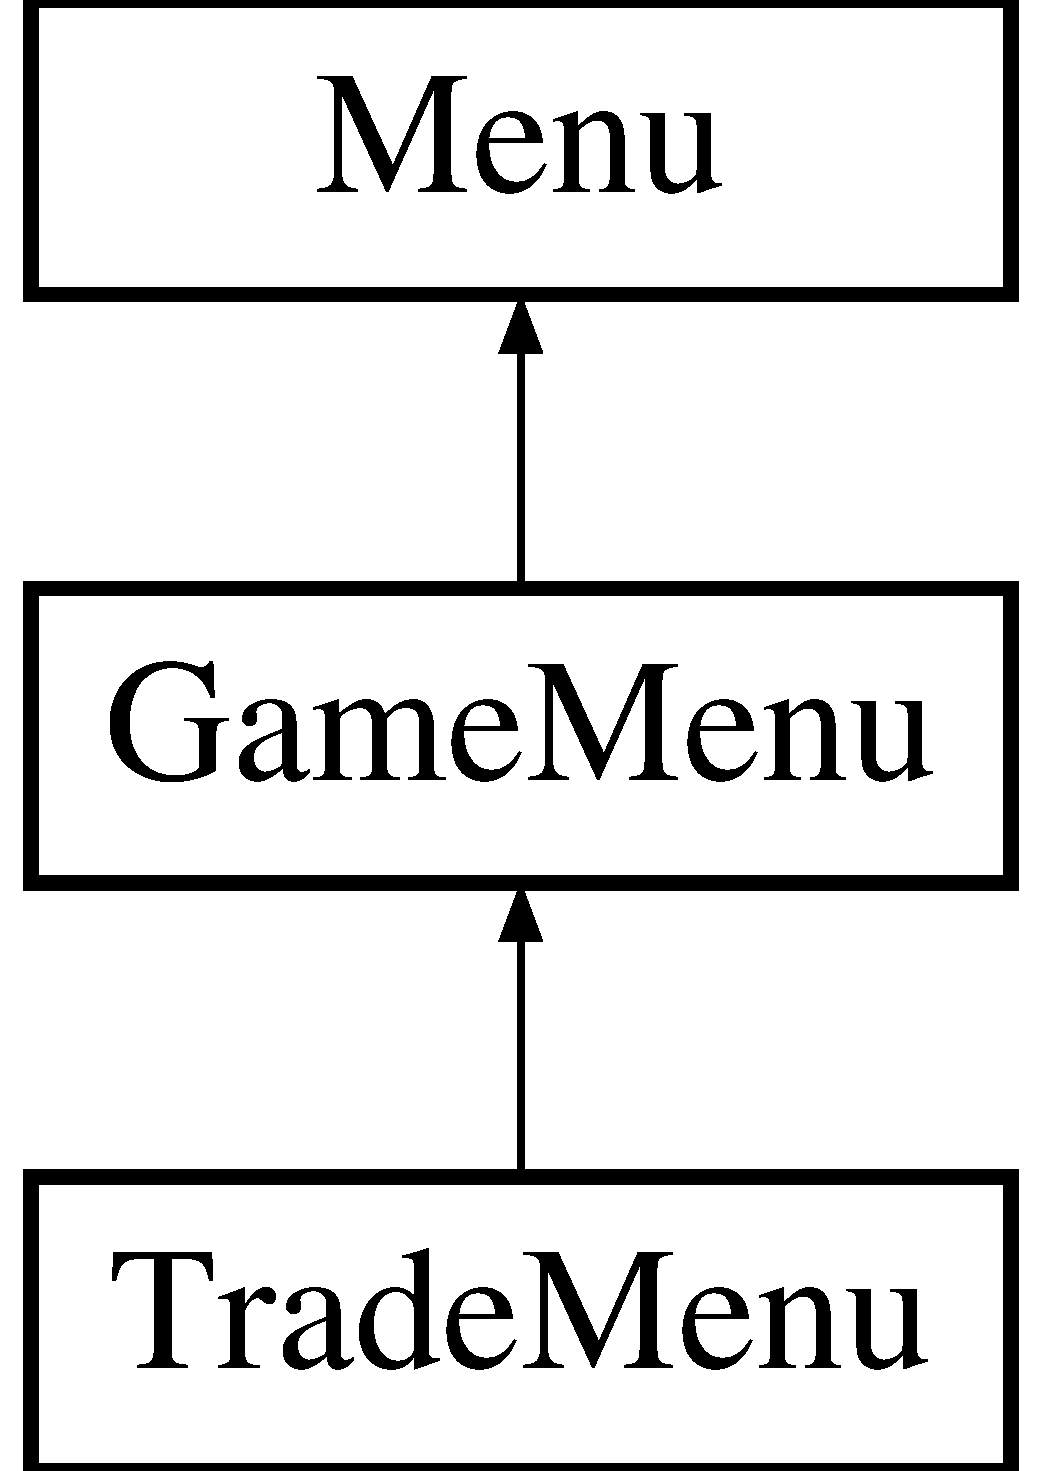
\includegraphics[height=3.000000cm]{classTradeMenu}
\end{center}
\end{figure}
\subsection*{Public Member Functions}
\begin{DoxyCompactItemize}
\item 
\hyperlink{classTradeMenu_a3b09de2db8d3b7a1f88fe9b62fe7b4ec}{Trade\-Menu} ()
\begin{DoxyCompactList}\small\item\em This is the default constructor. \end{DoxyCompactList}\item 
virtual \hyperlink{classTradeMenu_ac2cf70176a9ad343276dcaa6a4917e99}{$\sim$\-Trade\-Menu} ()
\begin{DoxyCompactList}\small\item\em This is the virtual destructor. \end{DoxyCompactList}\item 
virtual void \hyperlink{classTradeMenu_aaf93d0a5ee2574d2926bd22de278fb17}{Set\-Options} (int row, int col, int space)
\item 
virtual void \hyperlink{classTradeMenu_a367004a0b1ceccd4517de8dea1e1d210}{Handle\-Input} (istream \&is)
\end{DoxyCompactItemize}
\subsection*{Additional Inherited Members}


\subsection{Detailed Description}
This is the menu displayed when the player character is trading. 

\subsection{Constructor \& Destructor Documentation}
\hypertarget{classTradeMenu_a3b09de2db8d3b7a1f88fe9b62fe7b4ec}{\index{Trade\-Menu@{Trade\-Menu}!Trade\-Menu@{Trade\-Menu}}
\index{Trade\-Menu@{Trade\-Menu}!TradeMenu@{Trade\-Menu}}
\subsubsection[{Trade\-Menu}]{\setlength{\rightskip}{0pt plus 5cm}Trade\-Menu\-::\-Trade\-Menu (
\begin{DoxyParamCaption}
{}
\end{DoxyParamCaption}
)}}\label{classTradeMenu_a3b09de2db8d3b7a1f88fe9b62fe7b4ec}


This is the default constructor. 

\begin{DoxyDate}{Date}
25/10/2017 
\end{DoxyDate}
\begin{DoxyAuthor}{Author}
Tomas Rigaux
\end{DoxyAuthor}
This is the implementation for menu class for the player character to use when they are trading with N\-P\-Cs in the game. \hypertarget{classTradeMenu_ac2cf70176a9ad343276dcaa6a4917e99}{\index{Trade\-Menu@{Trade\-Menu}!$\sim$\-Trade\-Menu@{$\sim$\-Trade\-Menu}}
\index{$\sim$\-Trade\-Menu@{$\sim$\-Trade\-Menu}!TradeMenu@{Trade\-Menu}}
\subsubsection[{$\sim$\-Trade\-Menu}]{\setlength{\rightskip}{0pt plus 5cm}Trade\-Menu\-::$\sim$\-Trade\-Menu (
\begin{DoxyParamCaption}
{}
\end{DoxyParamCaption}
)\hspace{0.3cm}{\ttfamily [virtual]}}}\label{classTradeMenu_ac2cf70176a9ad343276dcaa6a4917e99}


This is the virtual destructor. 



\subsection{Member Function Documentation}
\hypertarget{classTradeMenu_a367004a0b1ceccd4517de8dea1e1d210}{\index{Trade\-Menu@{Trade\-Menu}!Handle\-Input@{Handle\-Input}}
\index{Handle\-Input@{Handle\-Input}!TradeMenu@{Trade\-Menu}}
\subsubsection[{Handle\-Input}]{\setlength{\rightskip}{0pt plus 5cm}void Trade\-Menu\-::\-Handle\-Input (
\begin{DoxyParamCaption}
\item[{istream \&}]{is}
\end{DoxyParamCaption}
)\hspace{0.3cm}{\ttfamily [virtual]}}}\label{classTradeMenu_a367004a0b1ceccd4517de8dea1e1d210}
This function handles the input for the menu options. 
\begin{DoxyParams}[1]{Parameters}
\mbox{\tt in,out}  & {\em is} & The in-\/stream operator to read the input. \\
\hline
\end{DoxyParams}


Implements \hyperlink{classGameMenu_a02ba09feedece5773f44ba865ccffb42}{Game\-Menu}.

\hypertarget{classTradeMenu_aaf93d0a5ee2574d2926bd22de278fb17}{\index{Trade\-Menu@{Trade\-Menu}!Set\-Options@{Set\-Options}}
\index{Set\-Options@{Set\-Options}!TradeMenu@{Trade\-Menu}}
\subsubsection[{Set\-Options}]{\setlength{\rightskip}{0pt plus 5cm}void Trade\-Menu\-::\-Set\-Options (
\begin{DoxyParamCaption}
\item[{int}]{row, }
\item[{int}]{col, }
\item[{int}]{space}
\end{DoxyParamCaption}
)\hspace{0.3cm}{\ttfamily [virtual]}}}\label{classTradeMenu_aaf93d0a5ee2574d2926bd22de278fb17}
This function sets the specific options for the \hyperlink{classMenu}{Menu} type. 
\begin{DoxyParams}[1]{Parameters}
\mbox{\tt in}  & {\em row} & Determines which row the options will start being set at. \\
\hline
\mbox{\tt in}  & {\em col} & Determines which column the options will start from. \\
\hline
\mbox{\tt in}  & {\em How} & mush space inbetween rows. \\
\hline
\end{DoxyParams}


Implements \hyperlink{classGameMenu_ac32ff465c5a4f30979e8851fa21cb230}{Game\-Menu}.



The documentation for this class was generated from the following files\-:\begin{DoxyCompactItemize}
\item 
/home/rigt2720/\-Kodika/\-Menu/\hyperlink{TradeMenu_8h}{Trade\-Menu.\-h}\item 
/home/rigt2720/\-Kodika/\-Menu/\hyperlink{TradeMenu_8cpp}{Trade\-Menu.\-cpp}\end{DoxyCompactItemize}

\hypertarget{classTradeState}{\section{Trade\-State Class Reference}
\label{classTradeState}\index{Trade\-State@{Trade\-State}}
}


Sets the state of the game when a player is 'trading' with an N\-P\-C. Derived from \hyperlink{classGameState}{Game\-State}.  




{\ttfamily \#include $<$Trade\-State.\-h$>$}

Inheritance diagram for Trade\-State\-:\begin{figure}[H]
\begin{center}
\leavevmode
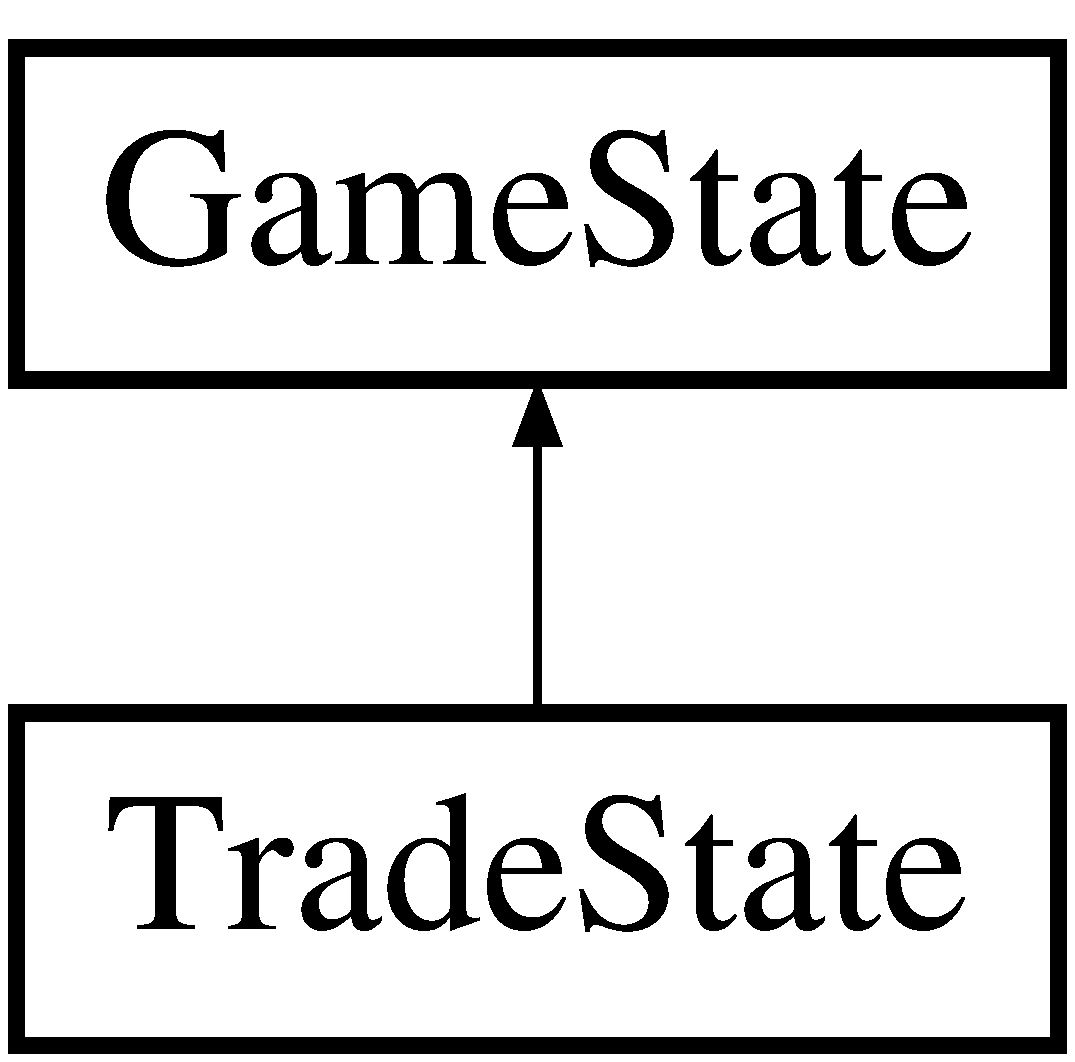
\includegraphics[height=2.000000cm]{classTradeState}
\end{center}
\end{figure}
\subsection*{Public Member Functions}
\begin{DoxyCompactItemize}
\item 
\hypertarget{classTradeState_a1778870265717d50054d29be886b27d4}{\hyperlink{classTradeState_a1778870265717d50054d29be886b27d4}{Trade\-State} ()}\label{classTradeState_a1778870265717d50054d29be886b27d4}

\begin{DoxyCompactList}\small\item\em Default constructor. \end{DoxyCompactList}\item 
\hypertarget{classTradeState_af0d9fdcd649c1e74620dc77a4b8f92f9}{void \hyperlink{classTradeState_af0d9fdcd649c1e74620dc77a4b8f92f9}{Set} ()}\label{classTradeState_af0d9fdcd649c1e74620dc77a4b8f92f9}

\begin{DoxyCompactList}\small\item\em Sets the layout of the game. \end{DoxyCompactList}\item 
\hypertarget{classTradeState_a6479e704b1063281721200a0beac6bc1}{void \hyperlink{classTradeState_a6479e704b1063281721200a0beac6bc1}{Get} ()}\label{classTradeState_a6479e704b1063281721200a0beac6bc1}

\begin{DoxyCompactList}\small\item\em Outputs the set layout. \end{DoxyCompactList}\end{DoxyCompactItemize}
\subsection*{Additional Inherited Members}


\subsection{Detailed Description}
Sets the state of the game when a player is 'trading' with an N\-P\-C. Derived from \hyperlink{classGameState}{Game\-State}. 

/date 21/10/2017 /author Tomas Rigaux

This is the state of the game when the player is trading with an N\-P\-C character. 

The documentation for this class was generated from the following file\-:\begin{DoxyCompactItemize}
\item 
Game\-State/Trade\-State.\-h\end{DoxyCompactItemize}

\hypertarget{classWeapon}{\section{Weapon Class Reference}
\label{classWeapon}\index{Weapon@{Weapon}}
}


This class is a abstract base class derived from \hyperlink{classItem}{Item} to represent weapons in game.  




{\ttfamily \#include $<$Weapon.\-h$>$}

Inheritance diagram for Weapon\-:\begin{figure}[H]
\begin{center}
\leavevmode
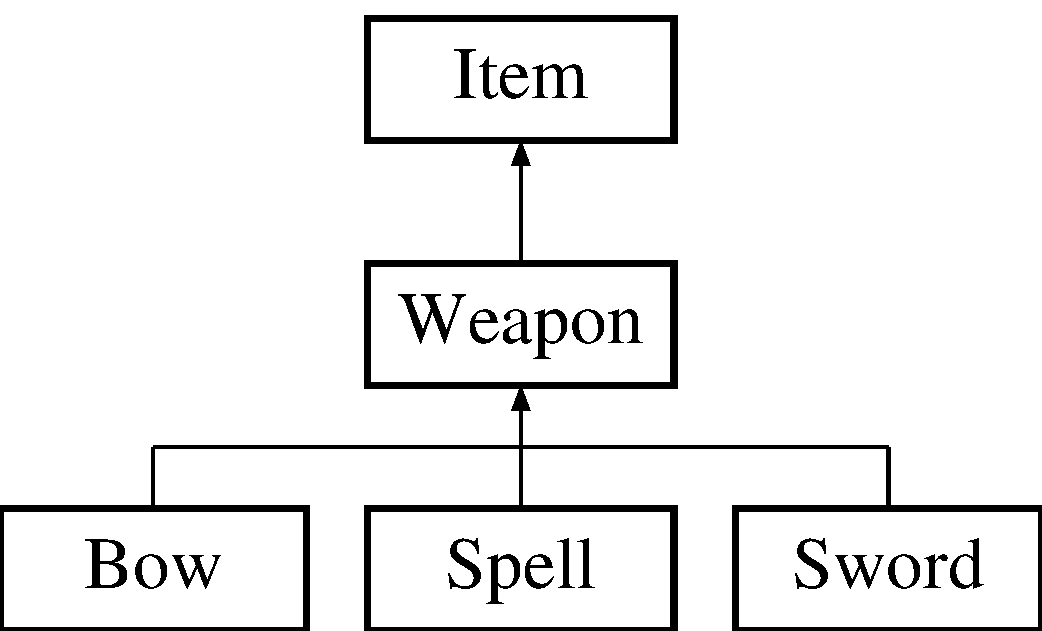
\includegraphics[height=3.000000cm]{classWeapon}
\end{center}
\end{figure}
\subsection*{Public Member Functions}
\begin{DoxyCompactItemize}
\item 
int \hyperlink{classWeapon_a1a74dac4314abc954c2f60d9ac204ae2}{base\-Damage} () const 
\begin{DoxyCompactList}\small\item\em read base damage \end{DoxyCompactList}\item 
int \& \hyperlink{classWeapon_afbc352ff3215793c073501859aa9c10d}{base\-Damage} ()
\begin{DoxyCompactList}\small\item\em write base damage \end{DoxyCompactList}\item 
int \hyperlink{classWeapon_a8f016a5f36802b05e92969f4a0d87649}{durability} () const 
\begin{DoxyCompactList}\small\item\em read durability \end{DoxyCompactList}\item 
int \& \hyperlink{classWeapon_a3557c5fa326d73478b97787ceaef532b}{durability} ()
\begin{DoxyCompactList}\small\item\em write durability \end{DoxyCompactList}\end{DoxyCompactItemize}
\subsection*{Protected Attributes}
\begin{DoxyCompactItemize}
\item 
int \hyperlink{classWeapon_a81c4f950298060a4b91c4170fc128631}{base\-Dmg}
\begin{DoxyCompactList}\small\item\em The Base damage of the weapon. \end{DoxyCompactList}\item 
int \hyperlink{classWeapon_abbc826be5477aa791910f871d76a1da2}{remaining\-Uses}
\begin{DoxyCompactList}\small\item\em How many more times the wepon can be used. \end{DoxyCompactList}\end{DoxyCompactItemize}
\subsection*{Additional Inherited Members}


\subsection{Detailed Description}
This class is a abstract base class derived from \hyperlink{classItem}{Item} to represent weapons in game. 

\subsection{Member Function Documentation}
\hypertarget{classWeapon_a1a74dac4314abc954c2f60d9ac204ae2}{\index{Weapon@{Weapon}!base\-Damage@{base\-Damage}}
\index{base\-Damage@{base\-Damage}!Weapon@{Weapon}}
\subsubsection[{base\-Damage}]{\setlength{\rightskip}{0pt plus 5cm}int Weapon\-::base\-Damage (
\begin{DoxyParamCaption}
{}
\end{DoxyParamCaption}
) const}}\label{classWeapon_a1a74dac4314abc954c2f60d9ac204ae2}


read base damage 

Returns the base damage of the weapon (for reading only) \begin{DoxyReturn}{Returns}
base damage of the weapon 
\end{DoxyReturn}
\hypertarget{classWeapon_afbc352ff3215793c073501859aa9c10d}{\index{Weapon@{Weapon}!base\-Damage@{base\-Damage}}
\index{base\-Damage@{base\-Damage}!Weapon@{Weapon}}
\subsubsection[{base\-Damage}]{\setlength{\rightskip}{0pt plus 5cm}int \& Weapon\-::base\-Damage (
\begin{DoxyParamCaption}
{}
\end{DoxyParamCaption}
)}}\label{classWeapon_afbc352ff3215793c073501859aa9c10d}


write base damage 

Returns the base damage of the weapon (for writing)  Reference to base\-Dmg \hypertarget{classWeapon_a8f016a5f36802b05e92969f4a0d87649}{\index{Weapon@{Weapon}!durability@{durability}}
\index{durability@{durability}!Weapon@{Weapon}}
\subsubsection[{durability}]{\setlength{\rightskip}{0pt plus 5cm}int Weapon\-::durability (
\begin{DoxyParamCaption}
{}
\end{DoxyParamCaption}
) const}}\label{classWeapon_a8f016a5f36802b05e92969f4a0d87649}


read durability 

Returns the number of times the weapon can be used (for reading only) \begin{DoxyReturn}{Returns}
number of remaining\-Uses 
\end{DoxyReturn}
\hypertarget{classWeapon_a3557c5fa326d73478b97787ceaef532b}{\index{Weapon@{Weapon}!durability@{durability}}
\index{durability@{durability}!Weapon@{Weapon}}
\subsubsection[{durability}]{\setlength{\rightskip}{0pt plus 5cm}int \& Weapon\-::durability (
\begin{DoxyParamCaption}
{}
\end{DoxyParamCaption}
)}}\label{classWeapon_a3557c5fa326d73478b97787ceaef532b}


write durability 

Returns the number of times the weapon can be used (for writing) \begin{DoxyReturn}{Returns}
a reference to remaining\-Uses 
\end{DoxyReturn}


\subsection{Member Data Documentation}
\hypertarget{classWeapon_a81c4f950298060a4b91c4170fc128631}{\index{Weapon@{Weapon}!base\-Dmg@{base\-Dmg}}
\index{base\-Dmg@{base\-Dmg}!Weapon@{Weapon}}
\subsubsection[{base\-Dmg}]{\setlength{\rightskip}{0pt plus 5cm}int Weapon\-::base\-Dmg\hspace{0.3cm}{\ttfamily [protected]}}}\label{classWeapon_a81c4f950298060a4b91c4170fc128631}


The Base damage of the weapon. 

\hypertarget{classWeapon_abbc826be5477aa791910f871d76a1da2}{\index{Weapon@{Weapon}!remaining\-Uses@{remaining\-Uses}}
\index{remaining\-Uses@{remaining\-Uses}!Weapon@{Weapon}}
\subsubsection[{remaining\-Uses}]{\setlength{\rightskip}{0pt plus 5cm}int Weapon\-::remaining\-Uses\hspace{0.3cm}{\ttfamily [protected]}}}\label{classWeapon_abbc826be5477aa791910f871d76a1da2}


How many more times the wepon can be used. 



The documentation for this class was generated from the following files\-:\begin{DoxyCompactItemize}
\item 
/home/rigt2720/\-Kodika/\-Item/\hyperlink{Weapon_8h}{Weapon.\-h}\item 
/home/rigt2720/\-Kodika/\-Item/\hyperlink{Weapon_8cpp}{Weapon.\-cpp}\end{DoxyCompactItemize}

%--- End generated contents ---

% Index
\newpage
\phantomsection
\addcontentsline{toc}{part}{Index}
\printindex

\end{document}
